\input{../style/preamble}
\input{../latex-math/basic-math}
\input{../latex-math/basic-ml}
\input{../latex-math/ml-nn}

% Macros and packages the DL4NLP source decks get from their own preamble
% (lecture_dl4nlp/style/preamble_new.tex) or per-file preambles.
\usepackage{animate}
\usepackage{xspace}
% The course's typewriter font (laett, set in dhbw-lecture.sty) has no bold shape;
% DL4NLP uses \textbf{\texttt{...}}, so map bold typewriter to regular.
\AtBeginDocument{{\ttfamily\selectfont}\DeclareFontShape{T1}{laett}{bx}{n}{<->ssub*laett/m/n}{}\DeclareFontShape{T1}{laett}{m}{bx}{<->ssub*laett/m/n}{}}
\newcommand{\citebutton}[2]{\beamergotobutton{\href{#2}{#1}}}
\newcommand{\ques}{\textbf{\textcolor{red}{Question:  }}}
\definecolor{texblue}{rgb}{0, 0, 1}
\def\myblue#1{\textcolor{texblue}{#1}}
\newcommand{\blu}[1]{\textcolor{blue}{#1}}
\newcommand{\org}[1]{\textcolor{orange}{#1}}
\long\def\devour#1{}
\newcommand\warning{%
 \makebox[1.4em][c]{%
 \makebox[0pt][c]{\raisebox{.1em}{\scriptsize!}}%
 \makebox[0pt][c]{\color{red}\normalsize$\bigtriangleup$}}}%

\def\cotpfull{chain-of-thought few-shot prompting\xspace}
\def\cotpfullcap{Chain-of-thought few-shot prompting\xspace}
\def\cotp{COT-FS-P\xspace}

\newcommand{\titlefigure}{figure/gptarch.png}
\newcommand{\learninggoals}{
  \item GPT-1 to GPT-3: generative pre-training, zero-/few-shot learning, capabilities and limitations
  \item Decoding: greedy and beam search, sampling strategies, decoding hyperparameters, evaluating generated text
  \item Fine-tuning and prompting: instruction tuning, multitask prompted training
  \item Chain-of-thought prompting and emergent abilities
  \item Reasoning models: DeepSeek-R1
}

\title{Advanced Artificial Intelligence and Machine Learning}
\date{}

\begin{document}

\lecturechapter{Large Language Models}
\lecture{Advanced AI \& ML}

%%%%%%%%%%%%%%%%%%%%%%%%%%%%%%%%%%%%%%%%%%%%%%%%%%%%%%%%%%%%%%%%%%
\section{GPT-1 (2018)}
% Source: DL4NLP chapter07-gpt/slides-71-gpt.tex
%%%%%%%%%%%%%%%%%%%%%%%%%%%%%%%%%%%%%%%%%%%%%%%%%%%%%%%%%%%%%%%%%%
% ------------------------------------------------------------------------------

\begin{frame}{GPT-1}

\vfill

	\begin{figure}
		\centering
		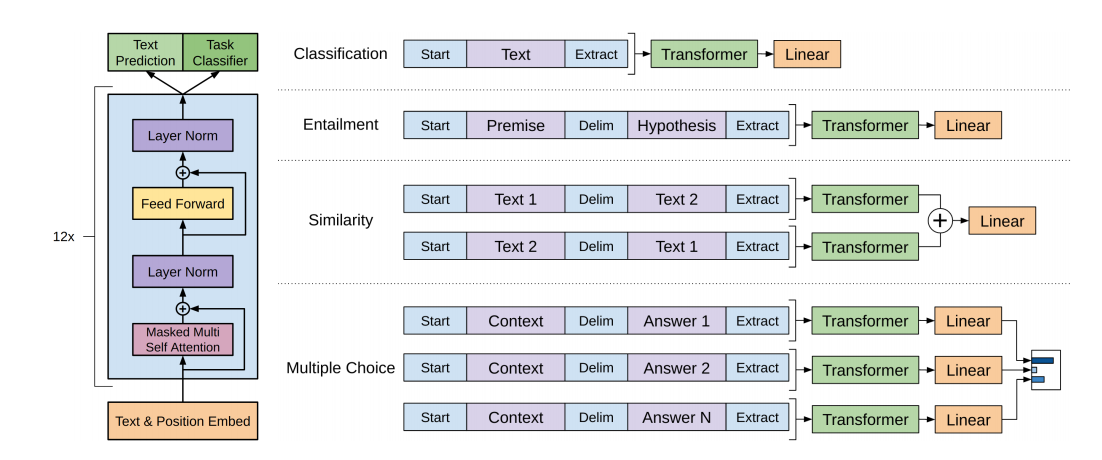
\includegraphics[width = 12cm]{figure/71-gpt}\\
		\citebutton{Source: Radford et al., 2018}{https://openai.com/blog/language-unsupervised/}
	\end{figure}

\vfill

\end{frame}

% ------------------------------------------------------------------------------

\begin{frame}{Architectural details}

\vfill

	\begin{itemize}
		\item Transformer \textit{decoder} as backbone of the architecture
			\begin{itemize}
				\item 12-layer-decoder with masked self-attention mechanism
				\item Hidden dimension $H = 768$, $A = 12$ Attention heads
				\item BPE vocabulary w/ 40k merges
				\item Learned positional embeddings (as opposed to fixed, sinusoidal ones in the original Transformer)
			\end{itemize}
		\item With $U = (w_{t-k}, \hdots, w_{t-1})$
\begin{align*}
	\vec h_0 &= \vec U \vec W_e + \vec W_p \\
	\vec h_l &= Trafo(\vec h_{l-1}) \forall l \in [1,n]\\
	P(w_t) &= softmax(\vec h_n \vec W_e^\top)
\end{align*}
	\end{itemize}

\vfill

\end{frame}

% ------------------------------------------------------------------------------

\begin{frame}{Pre-Training GPT}

\vfill

\begin{itemize}
		\item Standard LM objective

\begin{align*}
	L_1(\{w_1, \hdots, w_n\}) = \sum_i \log(P(w_t | w_{t-k}, \hdots, w_{t-1}; \Theta))
\end{align*}
					
					where $\{w_1, \hdots, w_n\}$ is an \textit{unlabeled} sequence of tokens

		\item \textit{Resource:} BooksCorpus 
			\begin{itemize}
				\item > 7k unpublished books from various genres
				\item contains long texts and thus allows learning long range dependencies
			\end{itemize}
\end{itemize}

\vfill

\end{frame}

% ------------------------------------------------------------------------------

\begin{frame}{Fine-Tuning GPT}

\vfill
			
\begin{itemize}
		\item Linear output layer with softmax activation on top
		\item Auxiliary language modeling objective during fine-tuning\\
					$\rightarrow$ Improves generalization\\
					$\rightarrow$ Accelerates convergence
		\item Task-specific input transformations
					\begin{itemize}
						\item \textit{Entailment:} \\ Concatenation of premise ($p$) \& hypothesis ($h$): $[p; \$; h]$
						\item \textit{Similarity:} Use both orderings and concatenate resulting representations: $[s_1; \$; s_2]$ and $[s_2; \$; s_1]$
						\item \textit{Q\&A and Commensense Reasoning:} \\ Concatenate context ($z$), question ($q$) and each possible answer ($a_k$): $[z; q; \$, a_k]$
					\end{itemize}
		\item Fine-tuning is rather quick, 3 epochs were sufficient
\end{itemize}

\vfill

\end{frame}

% ------------------------------------------------------------------------------

\begin{frame}{Fine-Tuning GPT}

\vfill

\begin{itemize}
		\item Additional objective:
					\begin{align*}
						L_2(\{w_1, \hdots, w_n\}) = \sum_{x,y} \log(P(y | w_1, \hdots, w_n))
					\end{align*}		
					where 
				\begin{itemize}
					\item $P(y | w_1, \hdots, w_n) = softmax(h_l^m W_y)$ and 
					\item $\{w_1, \hdots, w_n\}$ is a \textit{labeled} sequence of tokens
				\end{itemize}
		\item Combining both objectives: 
					\begin{align*}
						L_3(\{w_1, \hdots, w_n\}) = L_2(\{w_1, \hdots, w_n\}) + \lambda \cdot L_1(\{w_1, \hdots, w_n\})
					\end{align*}
\end{itemize}

\vfill

\end{frame}

% ------------------------------------------------------------------------------

\begin{frame}{SOTA results}

\vfill

	\textbf{Performance on different benchmarks:}

	\begin{figure}
		\centering
		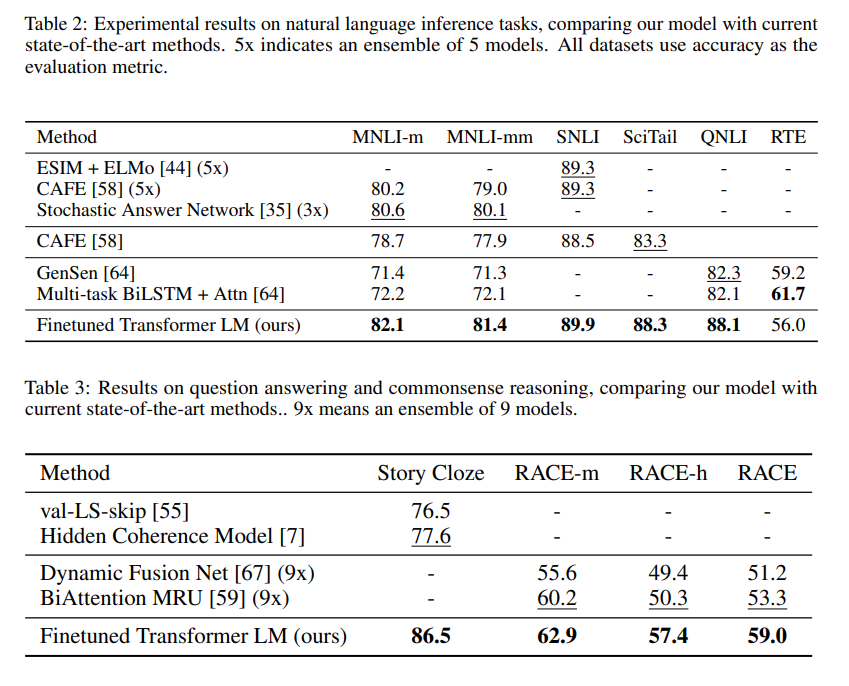
\includegraphics[width = 6.80cm]{figure/gpt-sota.png}\\ 
		\citebutton{Source: Radford et al., 2018}{https://openai.com/blog/language-unsupervised/}
	\end{figure}

\vfill

\end{frame}

% ------------------------------------------------------------------------------

\begin{frame}{GPT Parameter Count}

\vfill 

\begin{itemize}
	\item \textbf{We know}: 
		$$n_{layers} = 12; \quad d_{model} = 768; \quad V = 40000; \quad M = 512;$$
	\item \textbf{Also}: 
		$$N_{Decoder} = 12\cdot d_{model}^2 \quad and \quad  N_{Embedding} = \overbrace{V \times d_{model}}^{\text{token embedding}} + \underbrace{M \times d_{model}}_{\text{pos. embedding}}$$
	\end{itemize}

$$
\begin{aligned}
\Rightarrow \quad N_{total} &= n_{layers} \cdot N_{Decoder} + N_{Embedding} \\ 
&= 12\cdot 12\cdot 768^2 + 40000\times 768 + 512\times 768 \\
&= 116,047,872 \approx 117M
\end{aligned}
$$

\vfill
\textbf{Note that $N_{Decoder} = 12\cdot d_{model}^2$ and not $16 \cdot d_{model}^2$ because the Decoder here doesn't do cross attention!}
	
\end{frame}

% ------------------------------------------------------------------------------


%%%%%%%%%%%%%%%%%%%%%%%%%%%%%%%%%%%%%%%%%%%%%%%%%%%%%%%%%%%%%%%%%%
\section{GPT-2 (2019)}
% Source: DL4NLP chapter07-gpt/slides-72-gpt2.tex
%%%%%%%%%%%%%%%%%%%%%%%%%%%%%%%%%%%%%%%%%%%%%%%%%%%%%%%%%%%%%%%%%%
% ------------------------------------------------------------------------------

\begin{frame}{Starting with a controversy}

\vfill

\begin{figure}
\centering
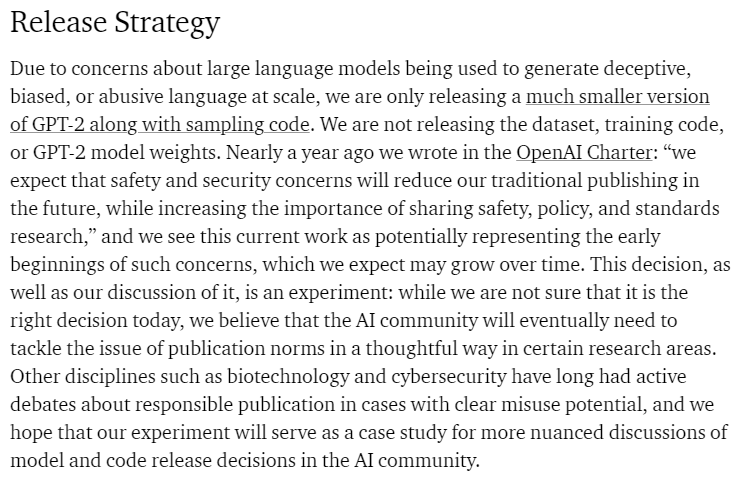
\includegraphics[width = 9cm]{figure/72-gpt2-release.png}\\ 
\citebutton{Source: OpenAI Blog}{https://openai.com/research/better-language-models}
\end{figure}

\vfill

\end{frame}

% ------------------------------------------------------------------------------

\begin{frame}{Capabilities -- Storytelling}

\vfill

\begin{figure}
\centering
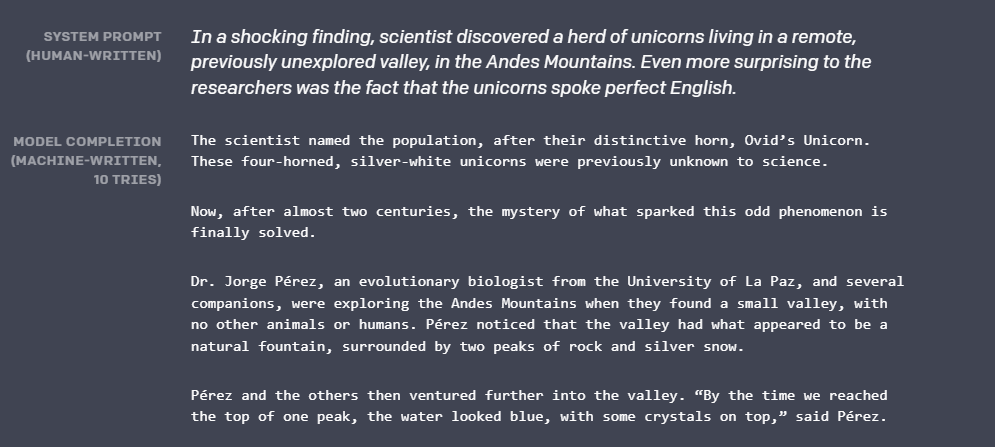
\includegraphics[width = 11cm]{figure/72-gpt2-story.png}\\ 
\citebutton{Source: OpenAI Blog}{https://openai.com/research/better-language-models}
\end{figure}

\vfill

\end{frame}

% ------------------------------------------------------------------------------

\begin{frame}{Capabilities -- Storytelling}

\vfill

\begin{figure}
\centering
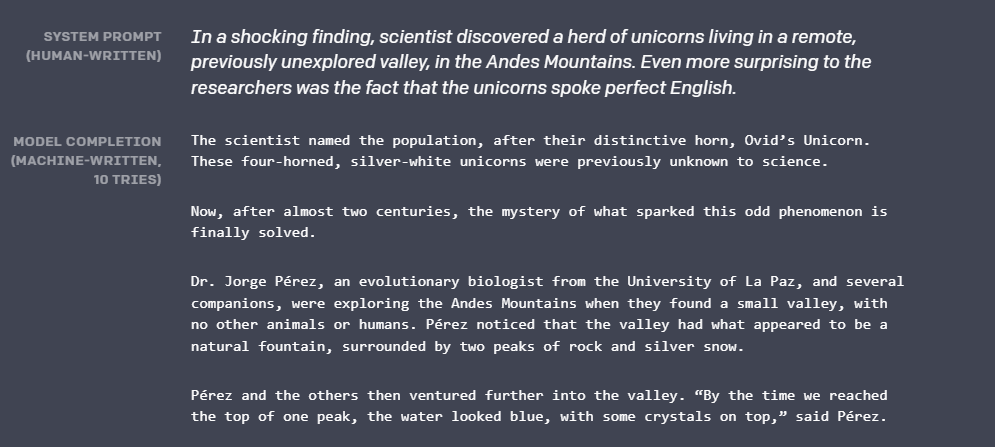
\includegraphics[width = 6cm]{figure/72-gpt2-story.png}\\ 
\citebutton{Source: OpenAI Blog}{https://openai.com/research/better-language-models}
\end{figure}

\begin{itemize}
	\item \textbf{In 2019:} Great achievement as the model is able to continue a made up story \textit{in a coherent way} by making up its own facts
	\item[] Sill: Not very consistent (``\texttt{four-horned [...] unicorns}``)
	\item \textbf{In 2023:} Nowadays this phenomenon is known as \textbf{hallucination} and a lot of research effort is put into mitigating this behaviour
\end{itemize}

\vfill

\end{frame}

% ------------------------------------------------------------------------------

\begin{frame}{The architecture}

\vfill

\begin{itemize}
	\item Transformer decoder pre-trained on AR language modeling
	\item Custom web scrape (not publicly available) of all outbound links from Reddit
	\item[$\to$] 8M documents / 40GB of text
	\item Byte-level BPE for tokenization
	\item Increased context size: $512 \to 1024$
\end{itemize}

\begin{figure}
\centering
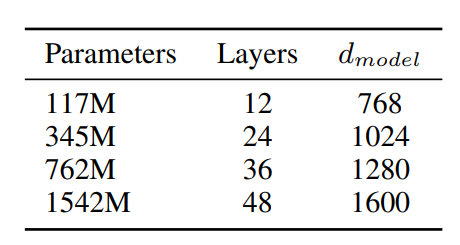
\includegraphics[width = 6cm]{figure/72-gpt2-size.png}\\ 
\citebutton{Source: Radford et al., 2019}{https://openai.com/research/better-language-models}
\end{figure}

\vfill

\end{frame}

% ------------------------------------------------------------------------------

\begin{frame}{Language models as multitask learners}

\vfill

\begin{itemize}

\item[] ``But as exemplified in McCann et al. (2018), language
	provides a flexible way to specify tasks, inputs,
	and outputs all as a sequence of symbols.

\item[] For
	example, a translation training
	example can be written as the sequence (translate to
	french, english text, french text).''
	\item Model benefits from seeing ``natural`` occurrences of task demonstrations during pre-training on large-scale web corpora
	\item[] $\to$ Related rationale to T5 (\textit{literal task descriptions}), but slightly different (\textit{acquired on the fly already during pre-training}).
\end{itemize}

\begin{figure}
\centering
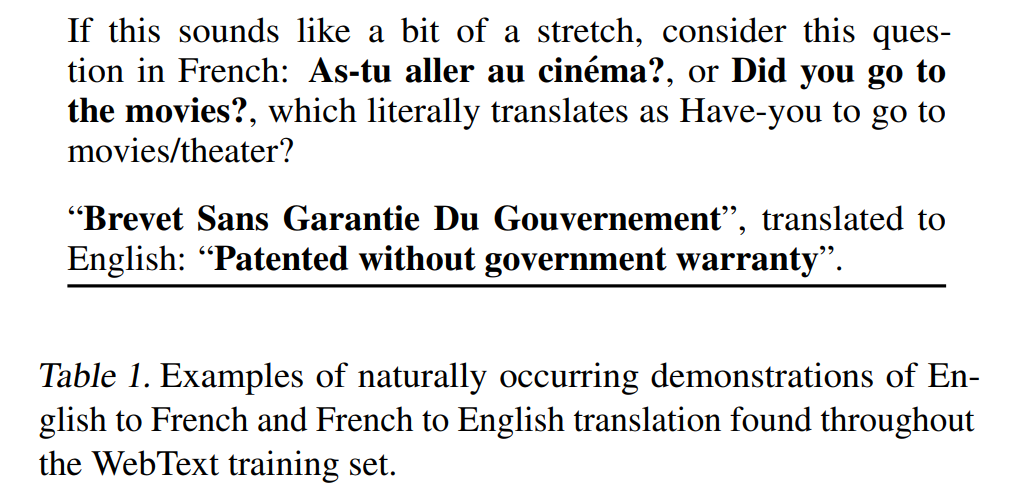
\includegraphics[width = 2.63cm]{figure/72-gpt2-demo-wild.png}\\ 
\citebutton{Source: Radford et al., 2019}{https://openai.com/research/better-language-models}
\end{figure}

\vfill

\end{frame}

% ------------------------------------------------------------------------------



\begin{frame}{Capabilities -- Zero-Shot}

\vfill

\begin{itemize}
	\item \textit{Zero-shot} refers to solving a task which the model was not previously explicitly trained on, just providing it with a description of the task but no demonstrations, i.e. input/output pairs.
	\item \textit{Few-shot} would be a relaxation of this setting, allowing for also providing the models with demonstrations (but still no training/gradient updates).
	\item Radford et al. show GPT-2's zero-shot capabilities on a range of different tasks, paving the way for the developments that came with GPT-3.
\end{itemize}

\vfill

\end{frame}

% ------------------------------------------------------------------------------

\begin{frame}{Capabilities -- Zero-Shot}

\vfill

\begin{figure}
\centering
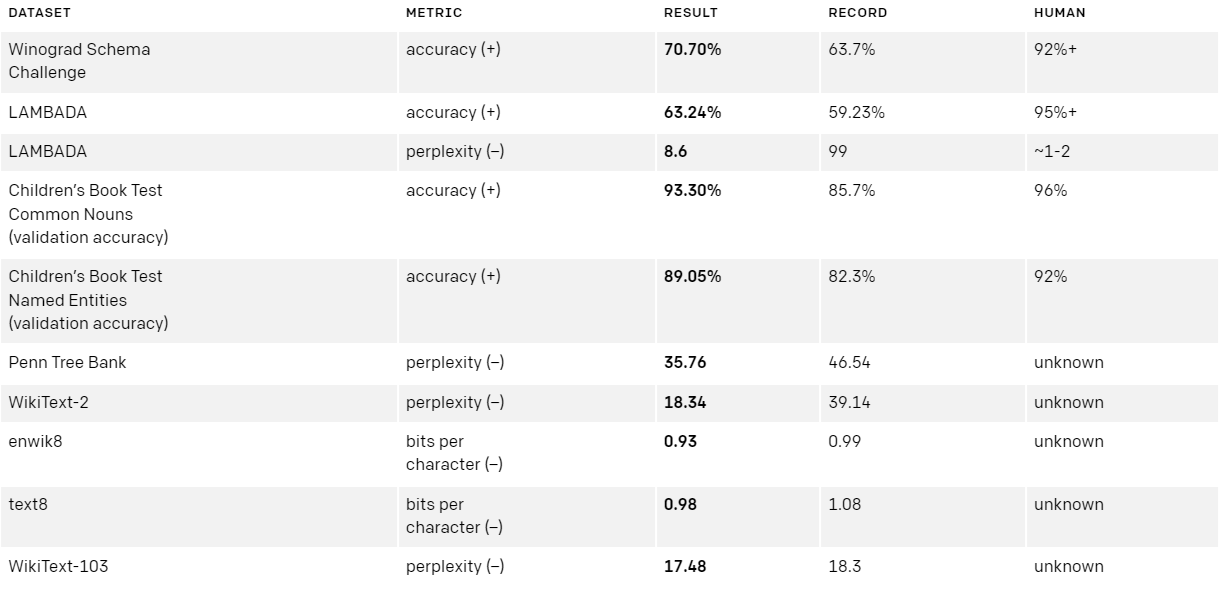
\includegraphics[width = 11cm]{figure/72-gpt2-zeroshot.png}\\ 
\citebutton{Source: Radford et al., 2019}{https://openai.com/research/better-language-models}
\end{figure}

\vfill

\footnotesize{(Note: The numbers correspond to the last row of the Table on slide 6)}

\end{frame}

% ------------------------------------------------------------------------------

\begin{frame}{Capabilities -- Factual knowledge}

\vfill

\textbf{Natural Questions} \citebutton{Kwiatkowski et al., 2019}{https://aclanthology.org/Q19-1026/}

\begin{itemize}
	\item Testing the \textit{factual knowledge} that is present in the pre-trained model
	\item Smallest model (117M): $< 1\%$
	\item GPT-2 (1542M): $4.1\%$
	\item[] $\to$ Model capacity as a major factor
	\item Calibration: High accuracy (63.1\%) on the 1\% most confident answers
\end{itemize}

\vfill

\end{frame}

% ------------------------------------------------------------------------------

\begin{frame}{Capabilities -- Factual knowledge}

\vfill

\textbf{The 30 most confident answers:}

\begin{figure}
\centering
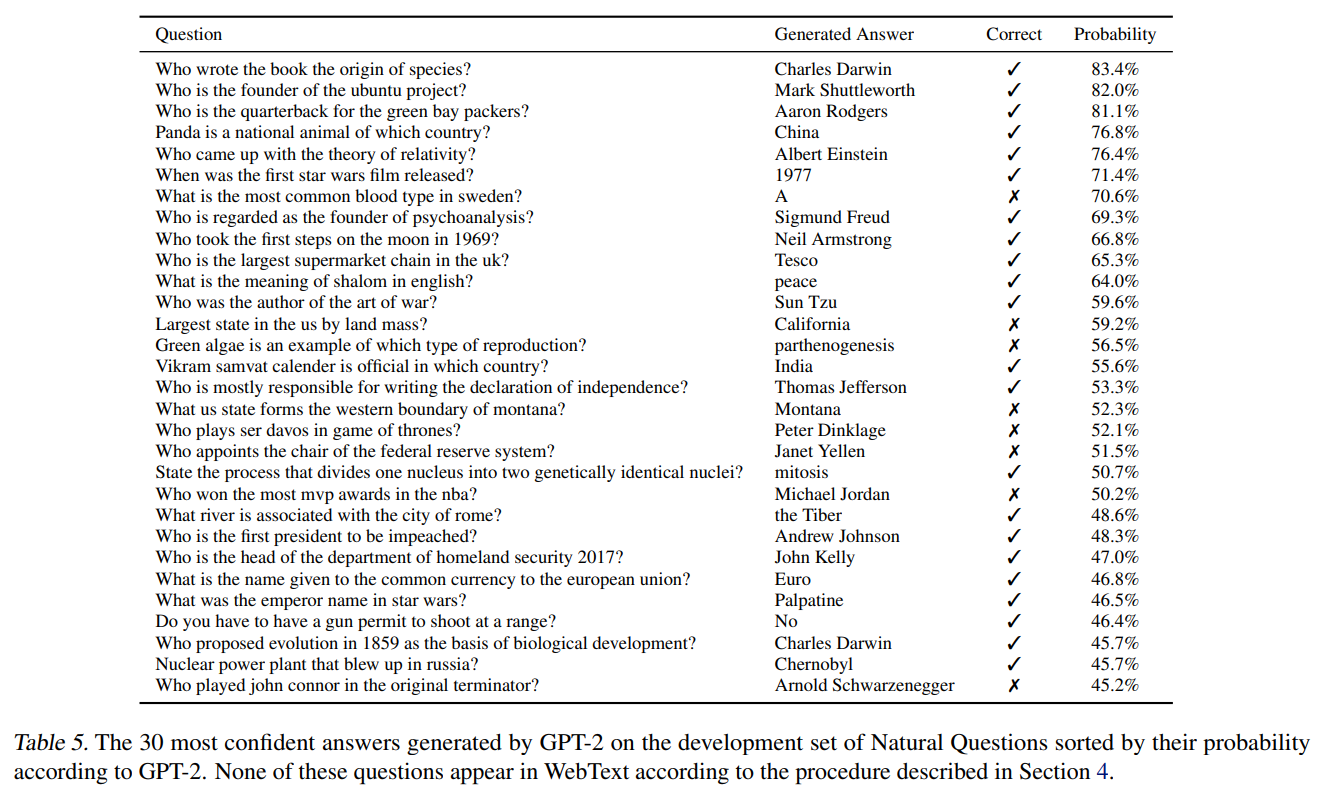
\includegraphics[width = 9.35cm]{figure/72-gpt2-qa.png}\\ 
\citebutton{Source: Radford et al., 2019}{https://openai.com/research/better-language-models}
\end{figure}

\vfill

\end{frame}

% ------------------------------------------------------------------------------

\begin{frame}{In the meantime}

\vfill

\begin{figure}
\centering
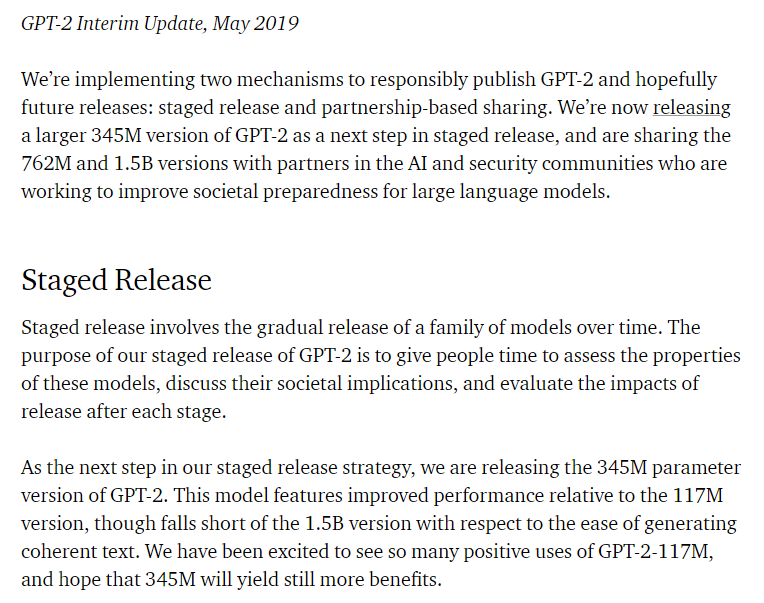
\includegraphics[width = 7.65cm]{figure/72-gpt2-release2.png}\\ 
\citebutton{Source: OpenAI Blog}{https://openai.com/research/better-language-models}
\end{figure}

\vfill

\end{frame}

% ------------------------------------------------------------------------------

\begin{frame}{In the meantime}

\vfill

\begin{itemize}
	\item Available on huggingface: \url{https://huggingface.co/gpt2}
	\item GPT-3 built on the foundation laid by GPT-2
	\item (also ChatGPT happened)
	\item GPT-2 (multi-task learning) extended to
	GPT-3 (prompting)
%        Prompting models has become more and more common\\ (cf. next chapter)
	\item Few-/Zero-Shot capabilites of models have become more important (cf. next chapter)
	\item Models of over $200\times$ the size of GPT-2 have been trained
	\item Transformer still the backbone of (nearly) all of them
\end{itemize}

\vfill

\end{frame}

% ------------------------------------------------------------------------------


%%%%%%%%%%%%%%%%%%%%%%%%%%%%%%%%%%%%%%%%%%%%%%%%%%%%%%%%%%%%%%%%%%
\section{GPT-3 (2020) \& X-shot Learning}
% Source: DL4NLP chapter07-gpt/slides-73-gpt3xshot.tex
%%%%%%%%%%%%%%%%%%%%%%%%%%%%%%%%%%%%%%%%%%%%%%%%%%%%%%%%%%%%%%%%%%
% ------------------------------------------------------------------------------

\begin{frame}{GPT recap}

\vfill

  \begin{itemize}
\item Like BERT, GPTs are called ``language models``.
\item Like BERT, GPTs are trained on huge corpora, actually on even huger (closed-source) corpora.
\item Like BERT, GPTs are based on the transformer architecture.
\item Unlike GPTs, BERT is \textit{not} a language model in the conventional sense, i.e. not an ARLM
\item BERT instead relies on the cloze taks, i.e. it is an MLM
\item GPTs are conventional ARLMs: they are just trained on predicting the next word (or subword).
    \end{itemize}

\vfill

\end{frame}

% ------------------------------------------------------------------------------

\begin{frame}{GPT recap}

\vfill

  \begin{itemize}
\item Difference 1: GPTs rely on the transformer decoder
\item[] $\to$ They are called ``\textit{generative}`` Large Language Models (LLM)
\item[] $\to$ BERT relies on the encoder, hence not perfectly suited for generation
\item Difference 2: GPT is a \myblue{single model} that aims to solve \myblue{all tasks}.  
  \begin{itemize}
    \item It can also switch back and forth between tasks and solve
    tasks within tasks, another human capability that is
    important in practice. \myblue{``fluidity''}
    \end{itemize}
\item Difference 3: GPT leverages \myblue{task descriptions}.
\item Difference 4: GPT is effective at \myblue{few-shot learning}.
    \end{itemize}

\vfill

\end{frame}

\begin{frame}{Prompting}

\vfill

  \begin{itemize}
\item Salesforce/GPT2: solve tasks by generation through
minor reformatting of original tasks (e.g., generate answer
in QA, generate label in classification)
\item Prompting: solve tasks by generation through carefully
designed prompts/instructions that are very different
from the original talk description.
\item Prompting is usually used within in-context learning
(zero-shot, one-shot, few-shot)
\item prompting = instruction = task description = pattern
    \end{itemize}

\vfill

\end{frame}

\begin{frame}{Schick (January 2020)}

\vfill

  \begin{itemize}
\item Arguably the first proposal of prompting with
language models
\item GPT3 published several months later
\item Schick \& Schuetze (2020):
Few-Shot Text Generation with Natural Language Instructions (arxiv)
    \end{itemize}

\vfill

\end{frame}

\begin{frame}{Schick (2020)}

\vfill

\begin{figure}
		\centering
		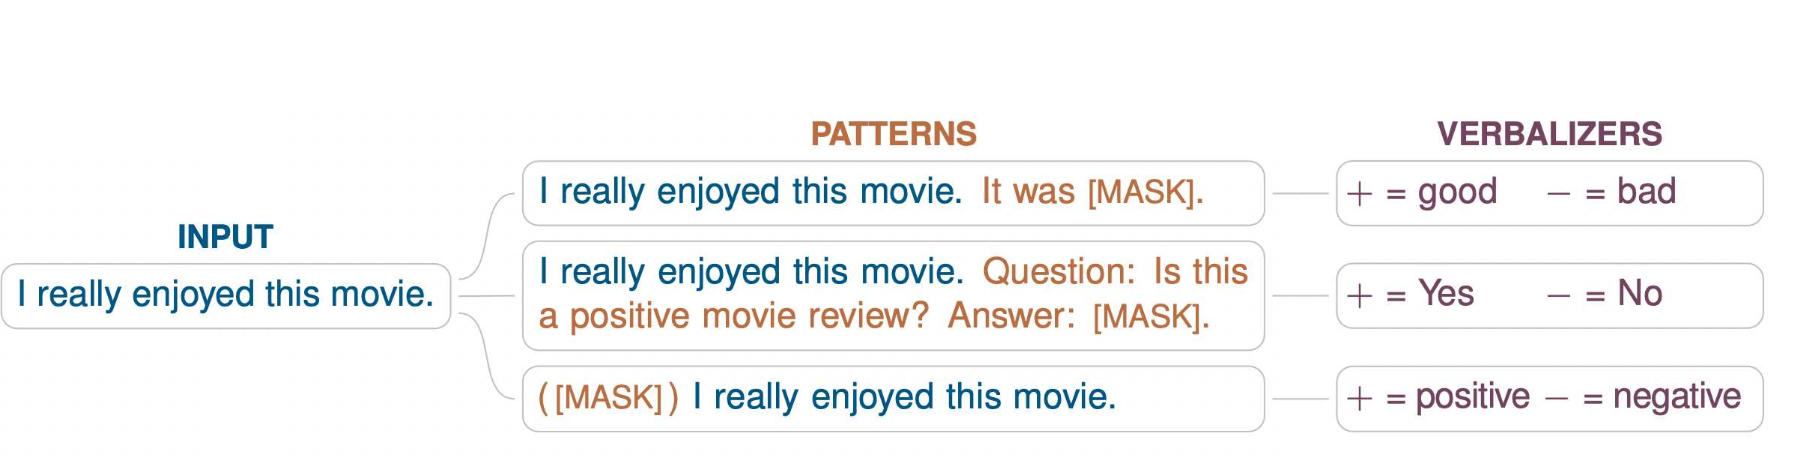
\includegraphics[width=\linewidth]{figure/schick.png}\\
		\citebutton{Source: Schick/Schuetze, 2020}{https://arxiv.org/pdf/2012.11926.pdf}
	\end{figure}

\vfill

\end{frame}

% ------------------------------------------------------------------------------

\begin{frame}{in-context learning}

\vfill

\begin{figure}
		\centering
		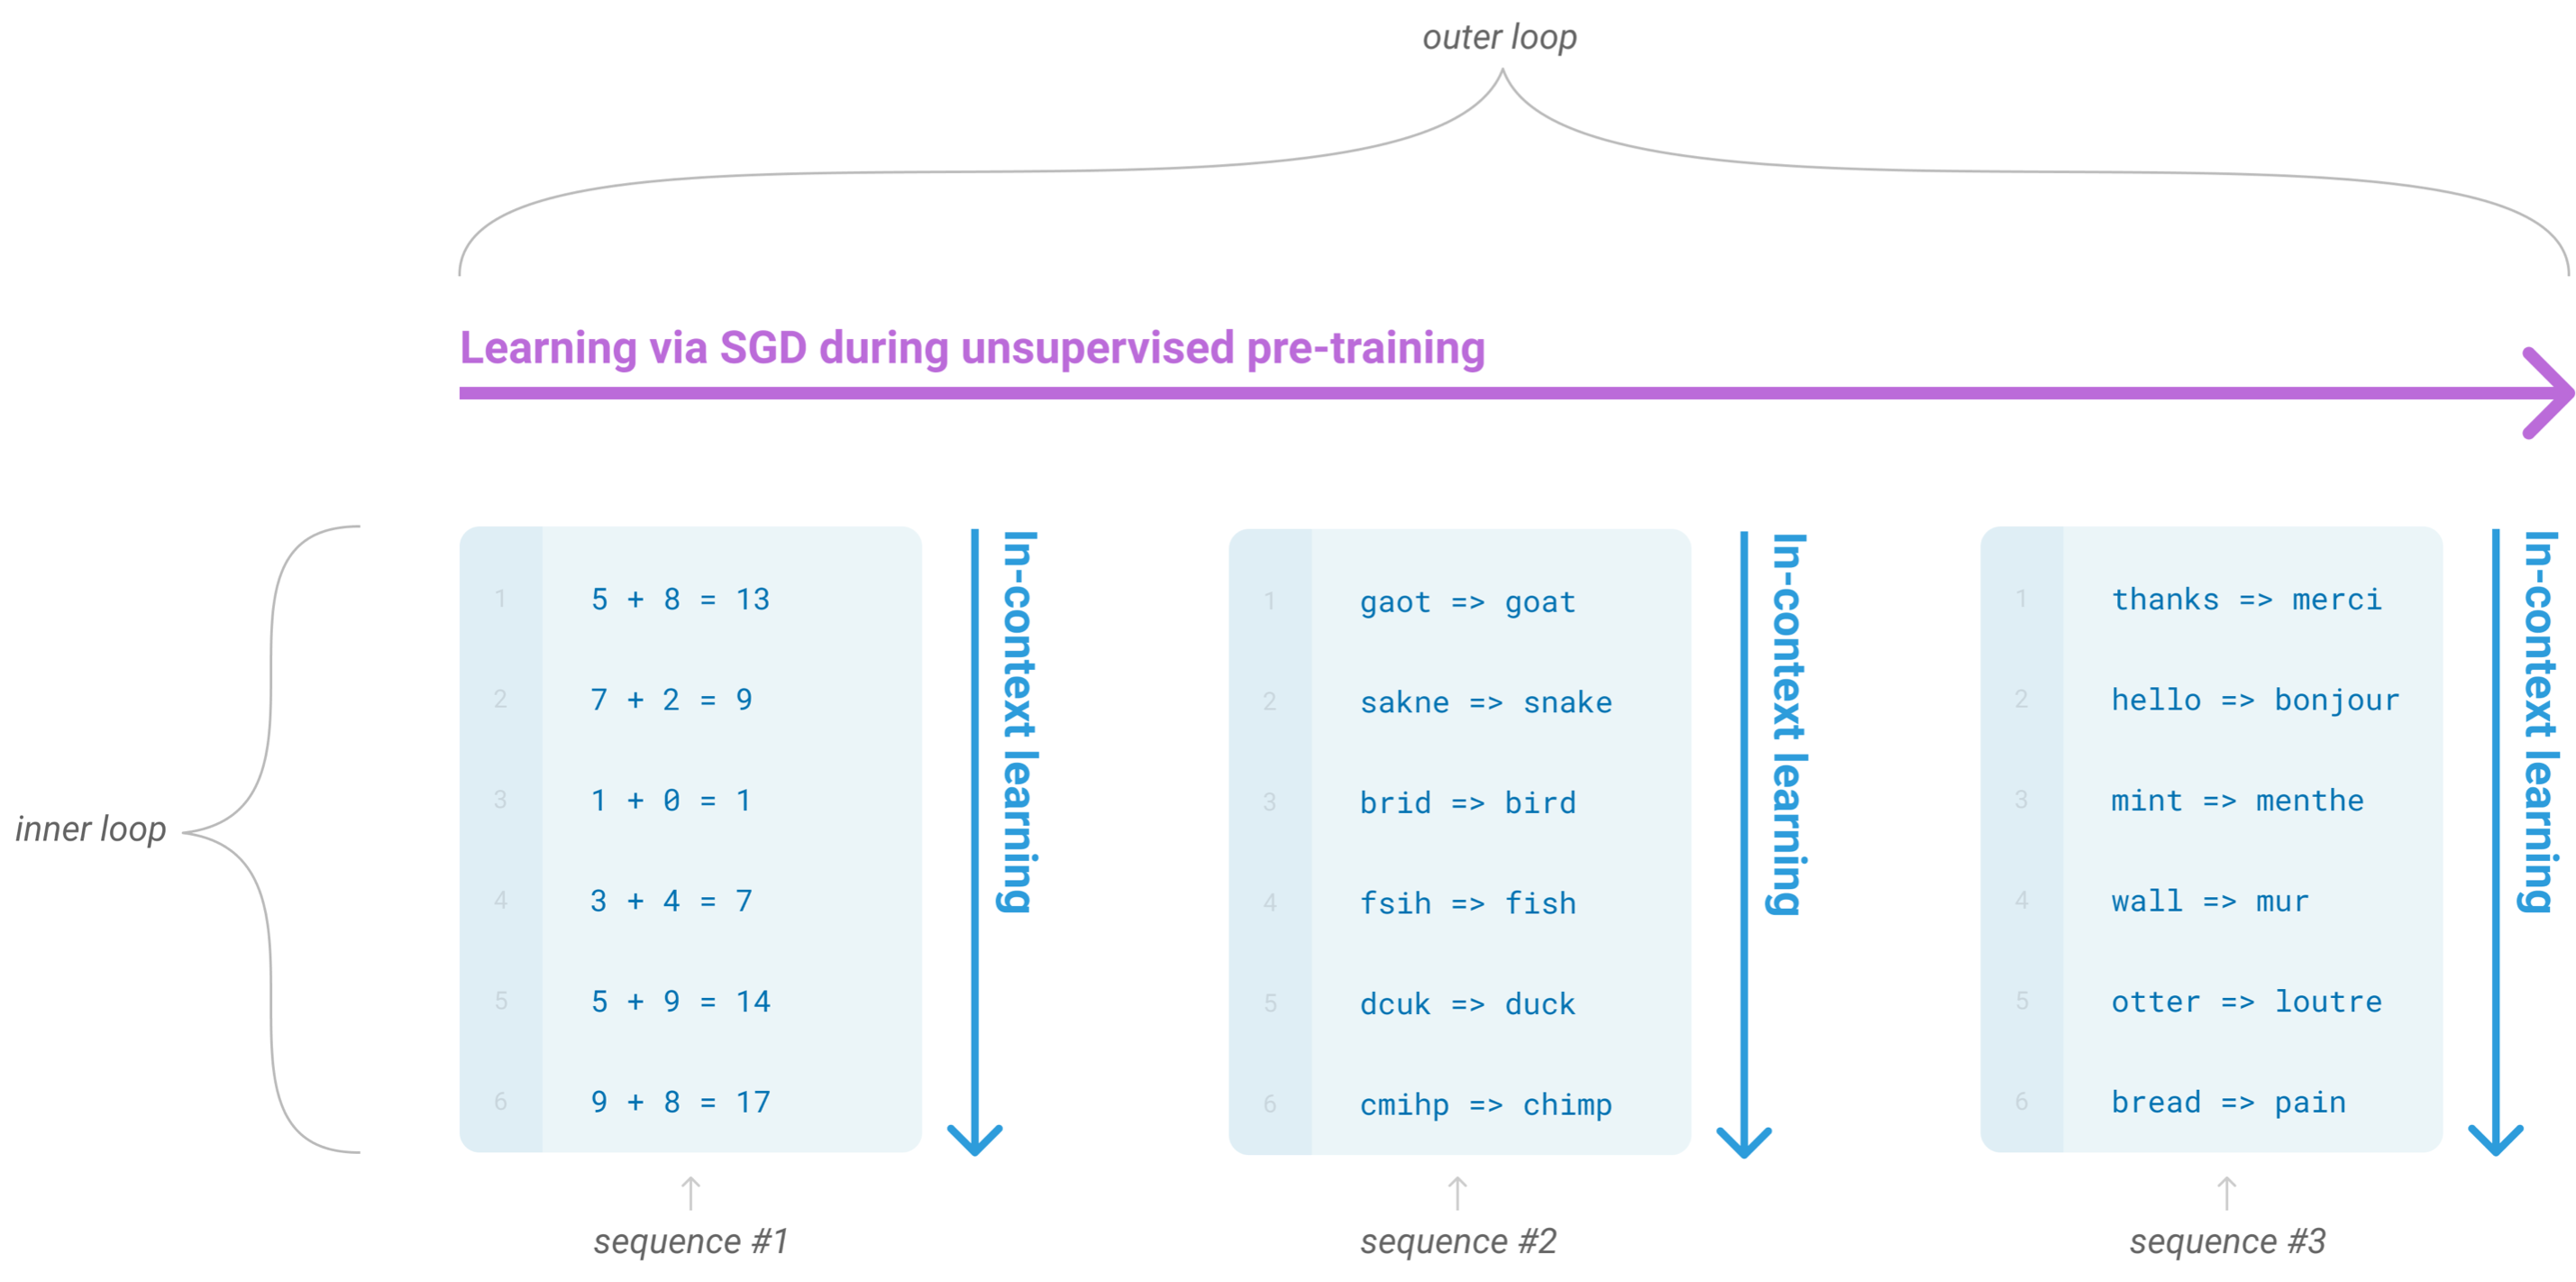
\includegraphics[clip,trim=200px 0 0 0,width=\linewidth]{figure/twotypesoflearning.png}\\
		\citebutton{Source: Brown et al., 2020}{https://arxiv.org/abs/2005.14165}
	\end{figure}

\vfill

\end{frame}

% ------------------------------------------------------------------------------

\begin{frame}{in-context learning}

\vfill

\begin{figure}
		\centering
		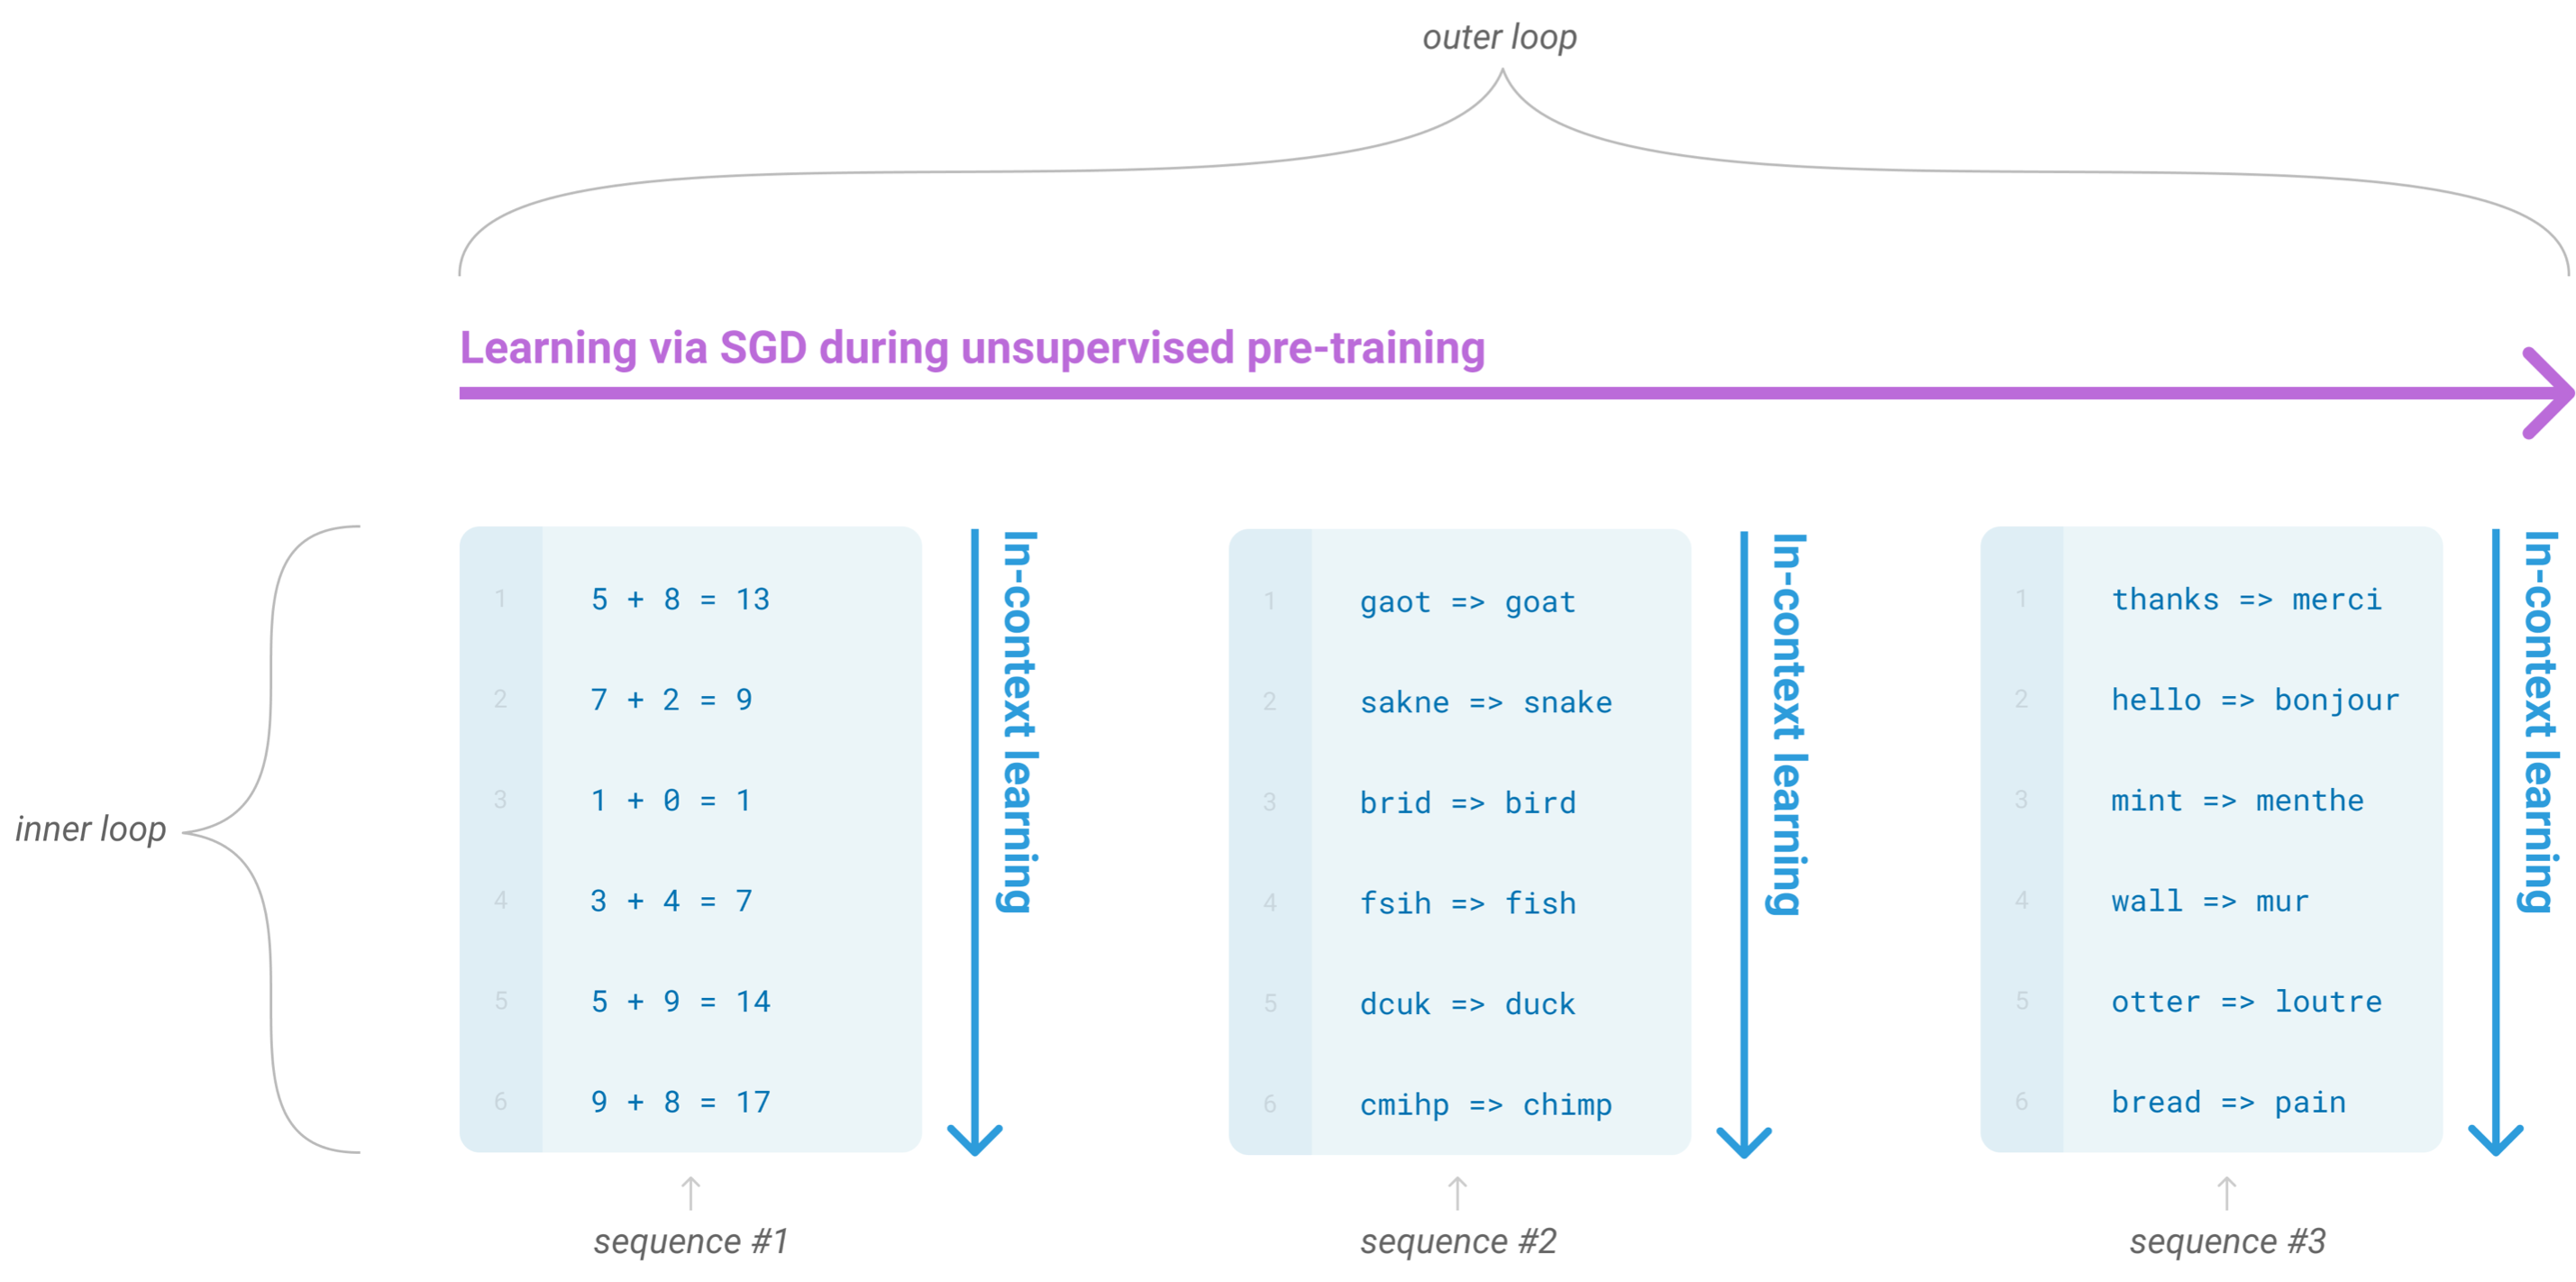
\includegraphics[width = 6cm]{figure/twotypesoflearning.png}\\
		\citebutton{Source: Brown et al., 2020}{https://arxiv.org/abs/2005.14165}
\end{figure}

\begin{itemize}
	\item \textbf{Pre-training (Outer loop):}
			\begin{itemize}
				\item Model develops broad set of skills and abilities
				\item Trained via gradient descent
			\end{itemize}
	\item \textbf{Inference (Inner loop):}
			\begin{itemize}
				\item It uses these abilities to rapidly adapt to a desired task\\(\textit{= in-context learning})
				\item Just a single forward pass w/o any gradient updates
			\end{itemize}
\end{itemize}

\vfill

\end{frame}

% ------------------------------------------------------------------------------

\begin{frame}{learning in bert \& co.}

\vfill

	\begin{figure}
		\centering
		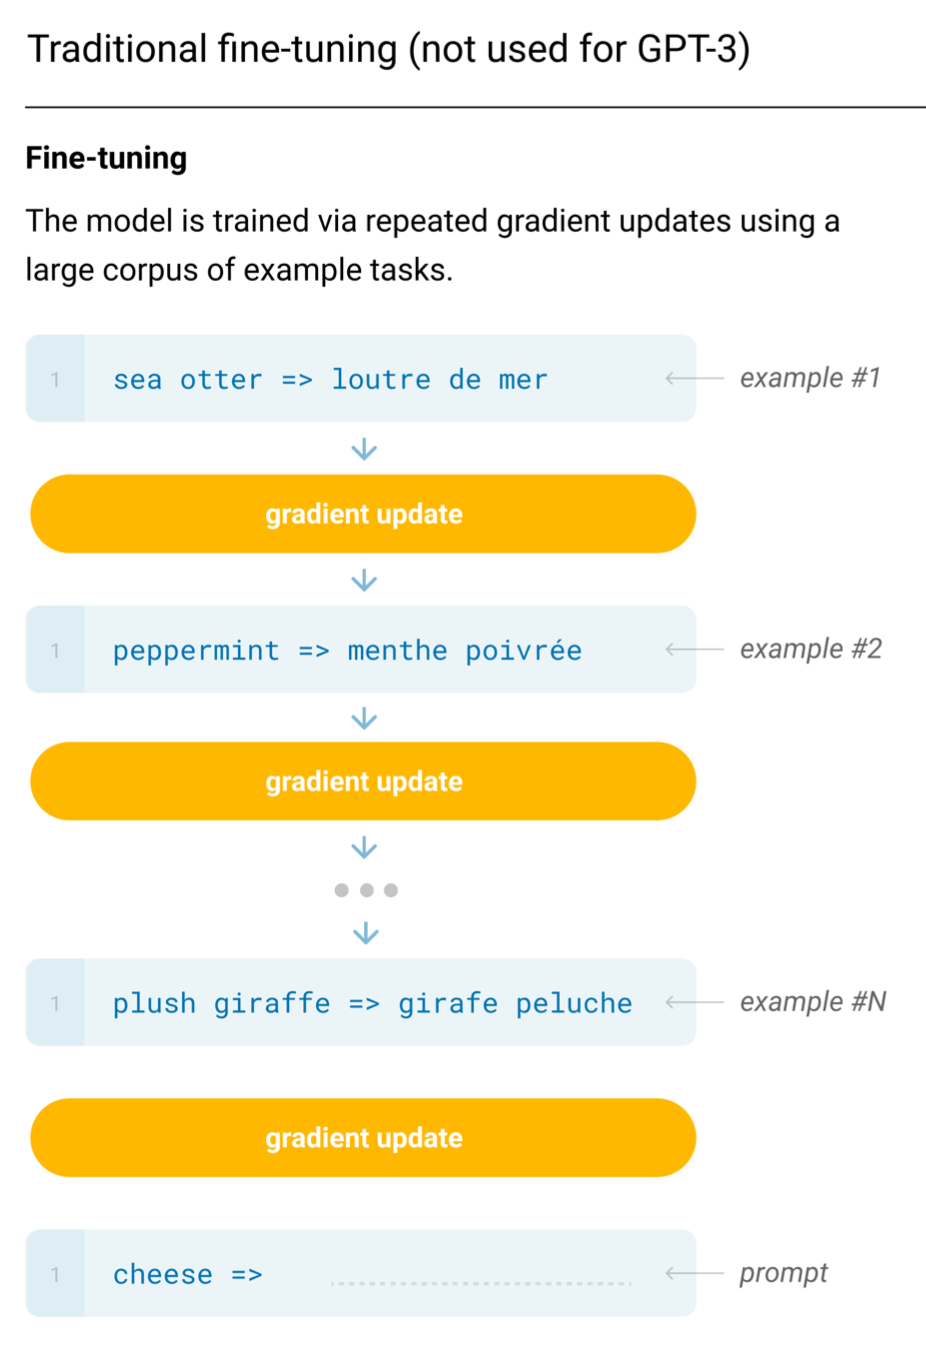
\includegraphics[width=4.25cm]{figure/gptnofinetuning.png}\\
		\citebutton{Source: Brown et al., 2020}{https://arxiv.org/abs/2005.14165}
	\end{figure}

\vfill

\end{frame}

% ------------------------------------------------------------------------------

\begin{frame}{Zero-shot learning}

\vfill

	\begin{figure}
		\centering
		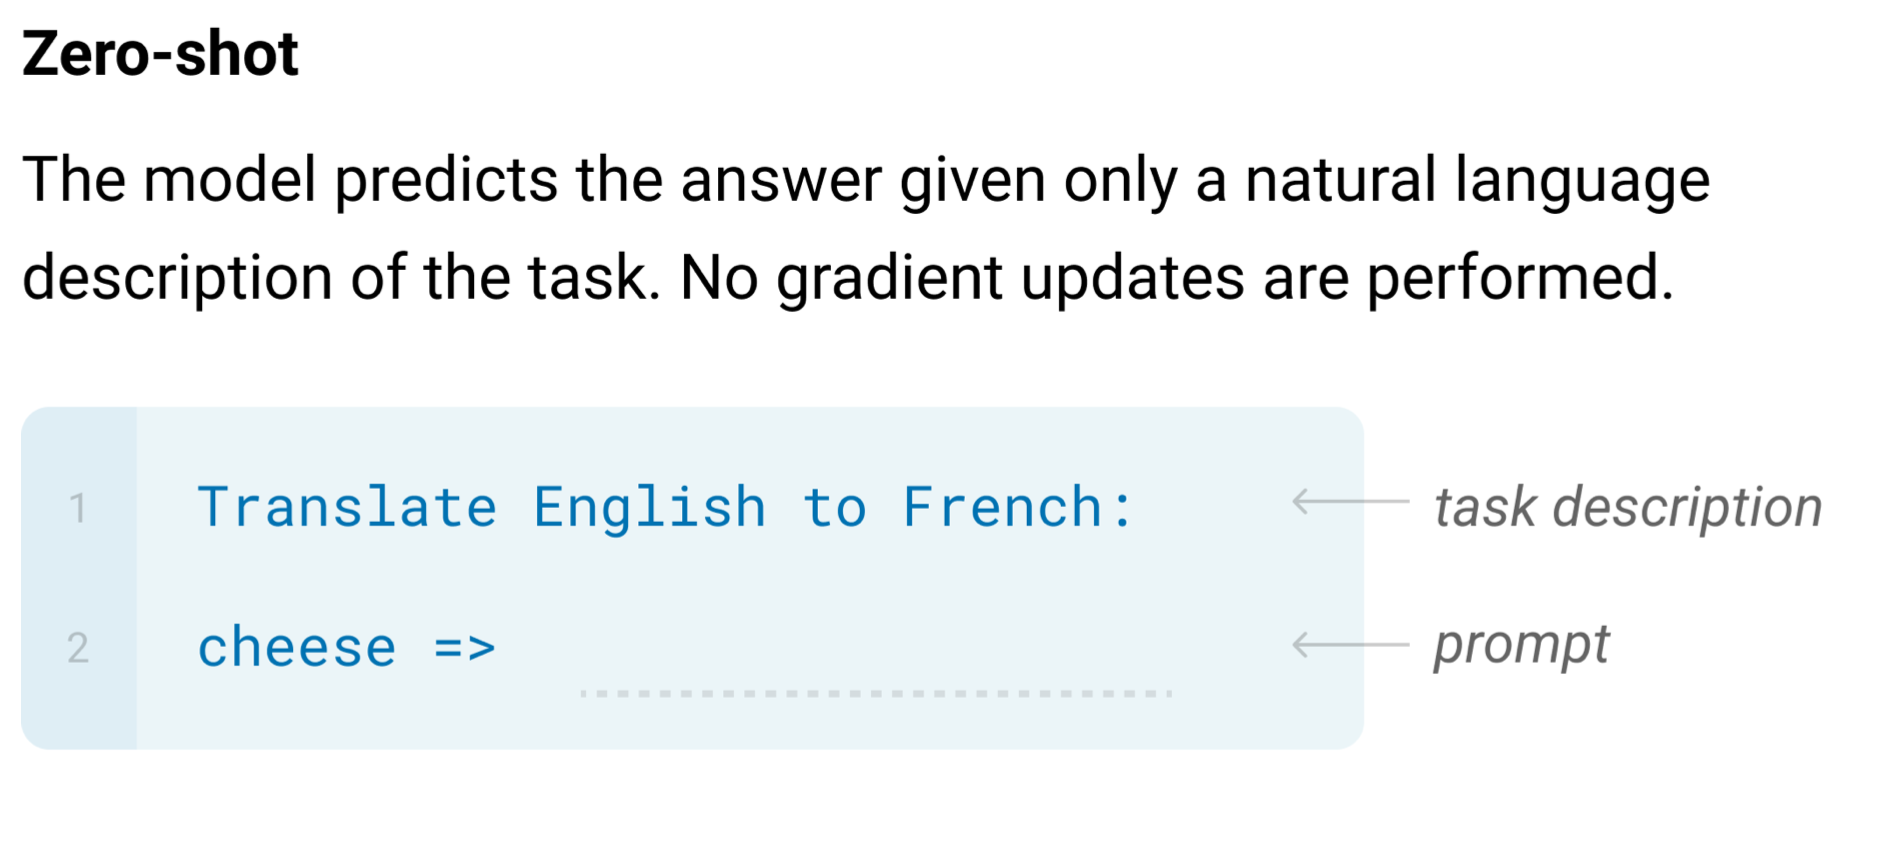
\includegraphics[width=10cm]{figure/gptzeroshot.png}\\
		\citebutton{Source: Brown et al., 2020}{https://arxiv.org/abs/2005.14165}
	\end{figure}

\begin{itemize}
	\item No gradient updates
	\item Learning happens ``on the fly``
	\item Model has to ``understand`` the task description
\end{itemize}

\vfill

\end{frame}

% ------------------------------------------------------------------------------

\begin{frame}{One-shot learning}

\vfill

	\begin{figure}
		\centering
		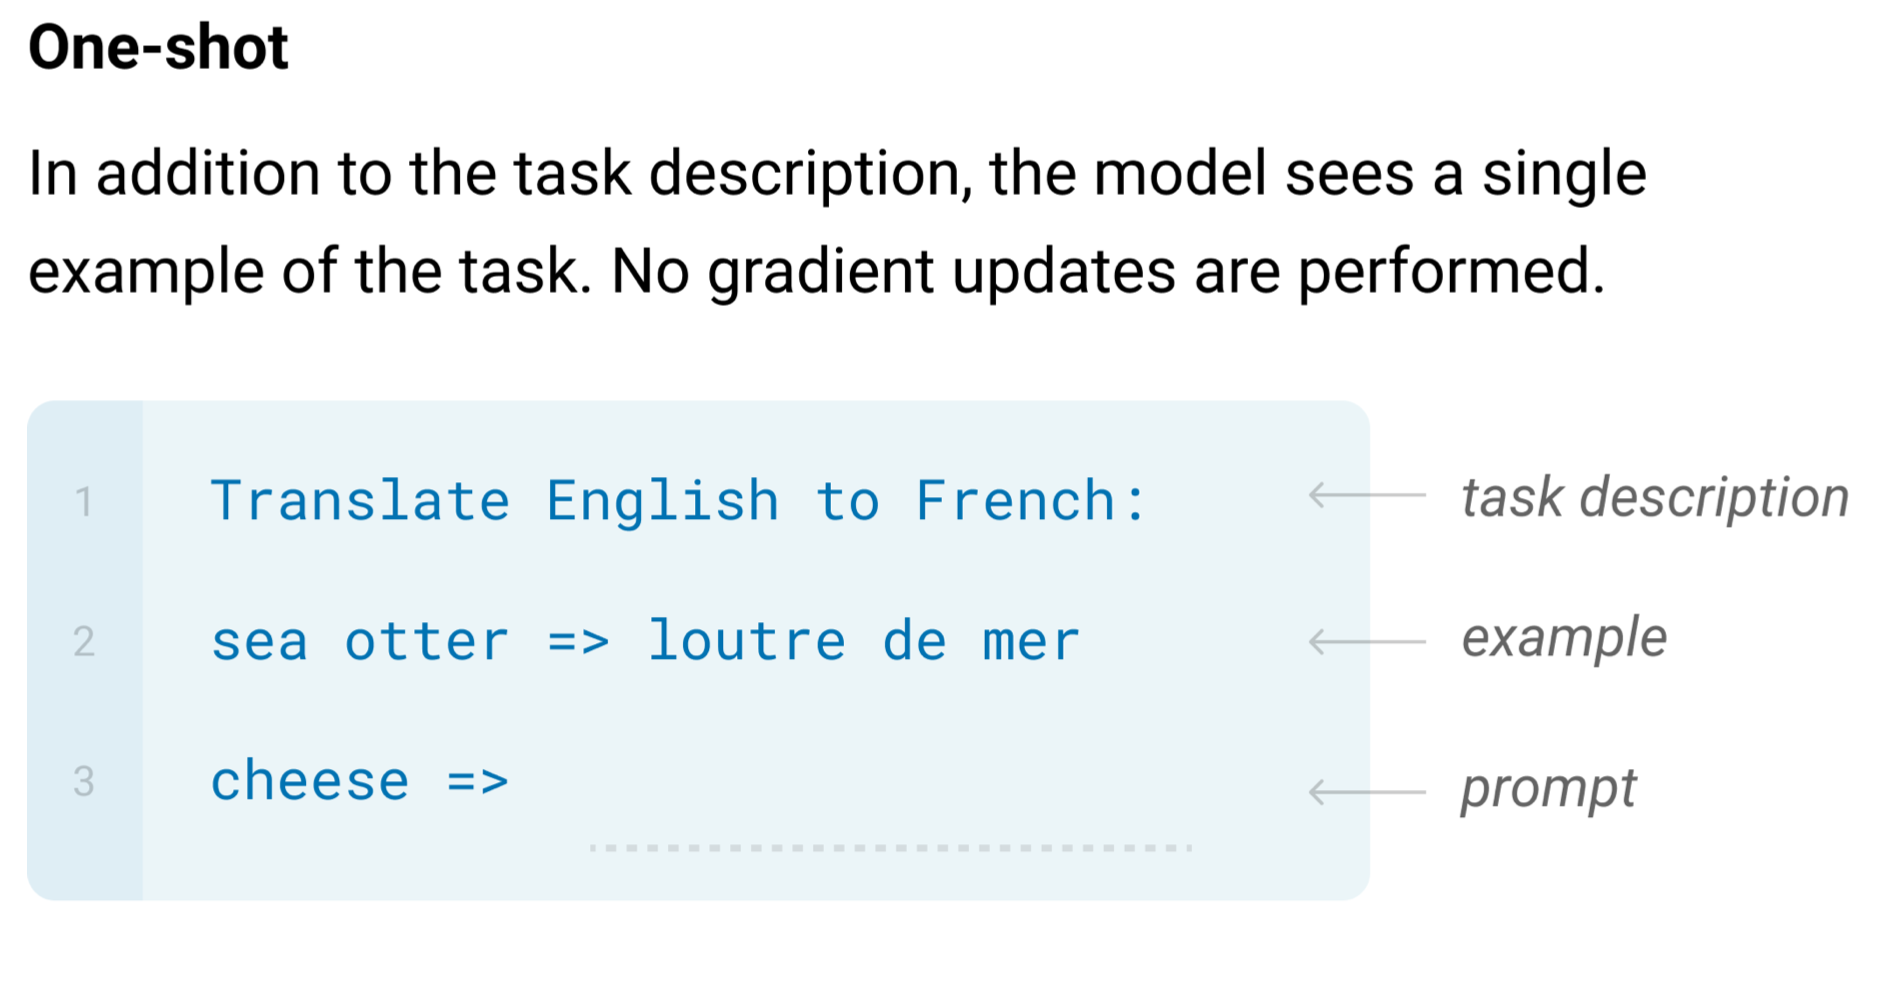
\includegraphics[width=8.50cm]{figure/gptoneshot.png}\\
		\citebutton{Source: Brown et al., 2020}{https://arxiv.org/abs/2005.14165}
	\end{figure}

\begin{itemize}
	\item No gradient updates
	\item Model has to ``understand`` the task description
	\item Understanding supported by \textit{one} demonstration
\end{itemize}

\vfill

\end{frame}

% ------------------------------------------------------------------------------

\begin{frame}{Few-shot learning}

\vfill

	\begin{figure}
		\centering
		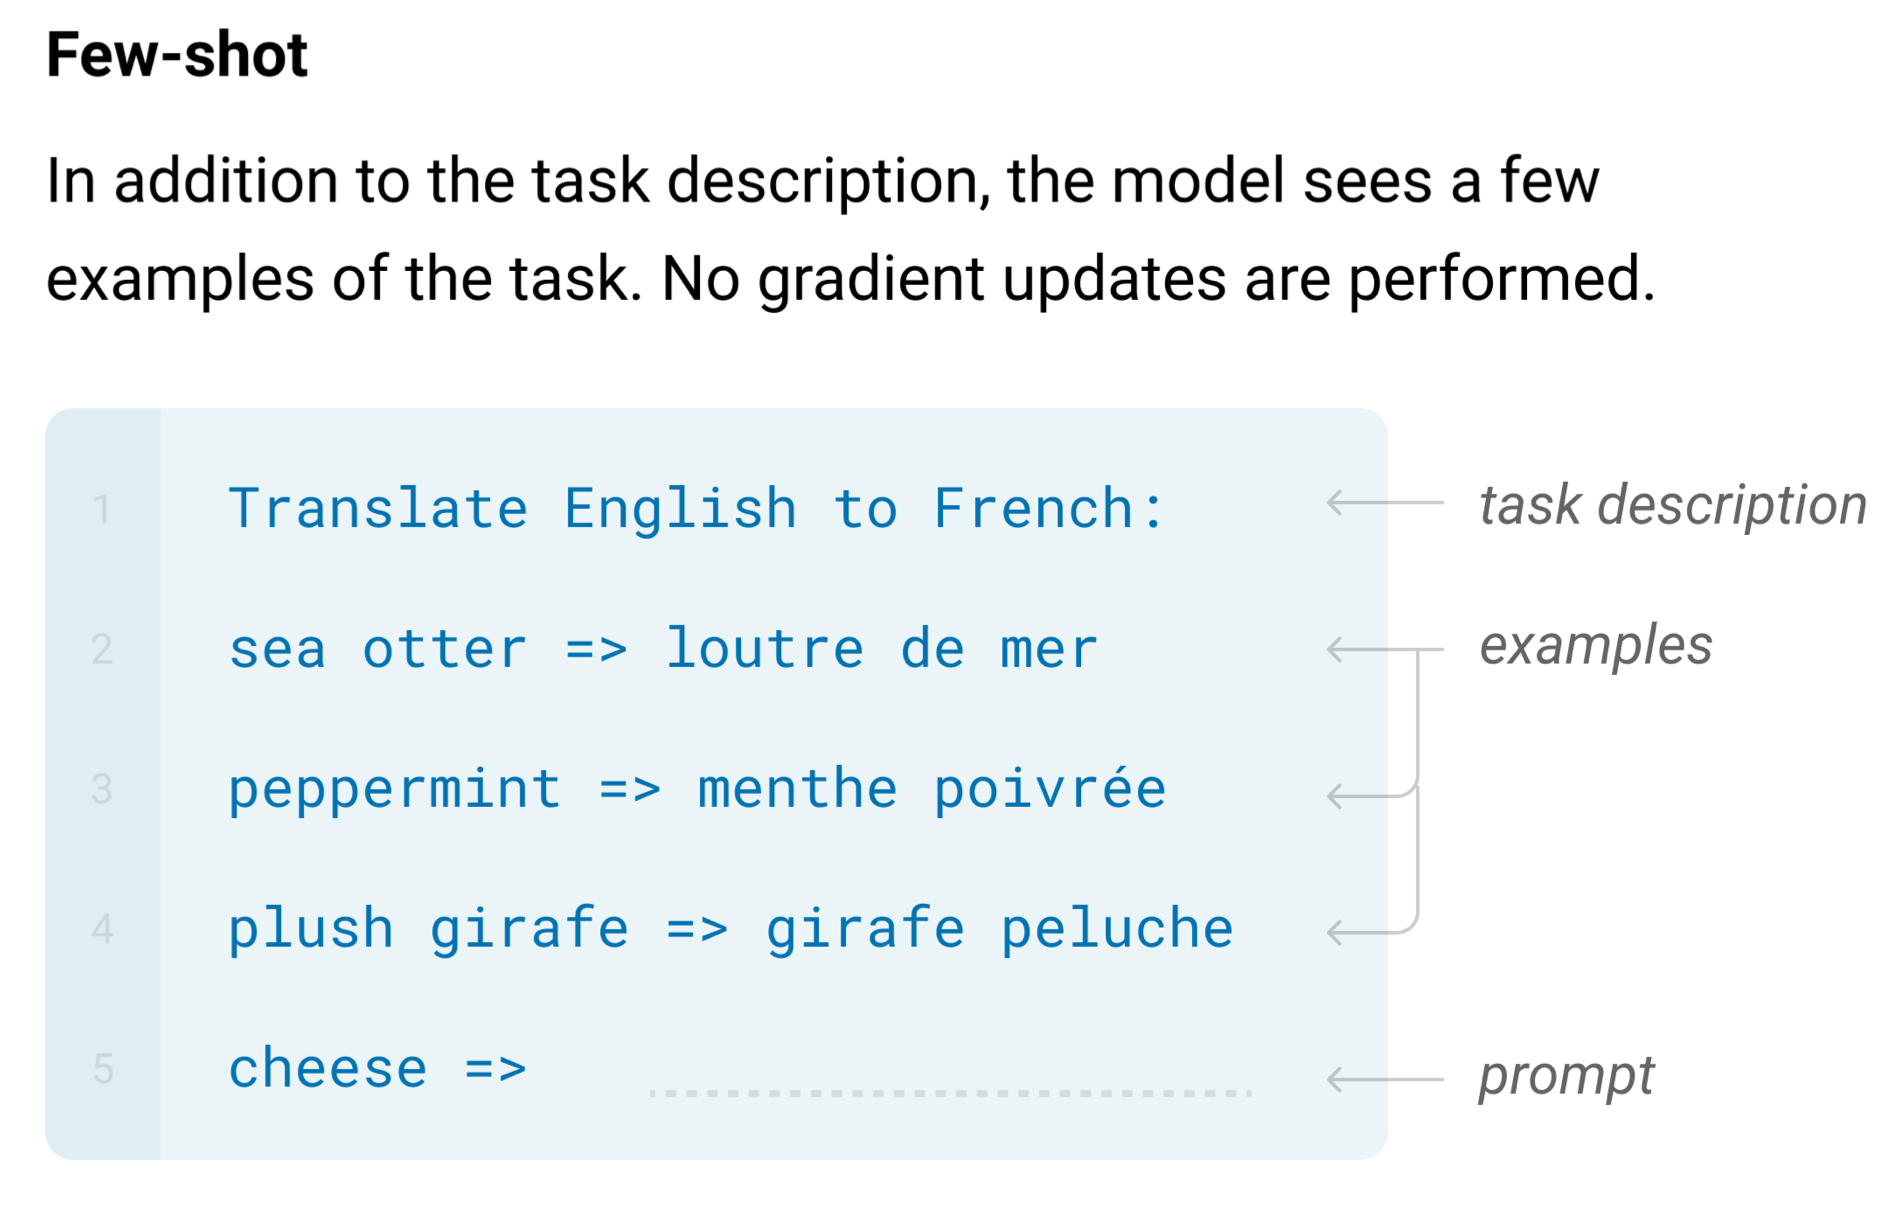
\includegraphics[width=6.80cm]{figure/gptfewshot.png}\\
		\citebutton{Source: Brown et al., 2020}{https://arxiv.org/abs/2005.14165}
	\end{figure}

\begin{itemize}
	\item No gradient updates
	\item Model has to ``understand`` the task description
	\item Understanding supported by \textit{few} demonstrations
\end{itemize}

\vfill

\end{frame}

% ------------------------------------------------------------------------------

\begin{frame}{effective in-context learning*}
	
\vfill
	
\begin{figure}
		\centering
		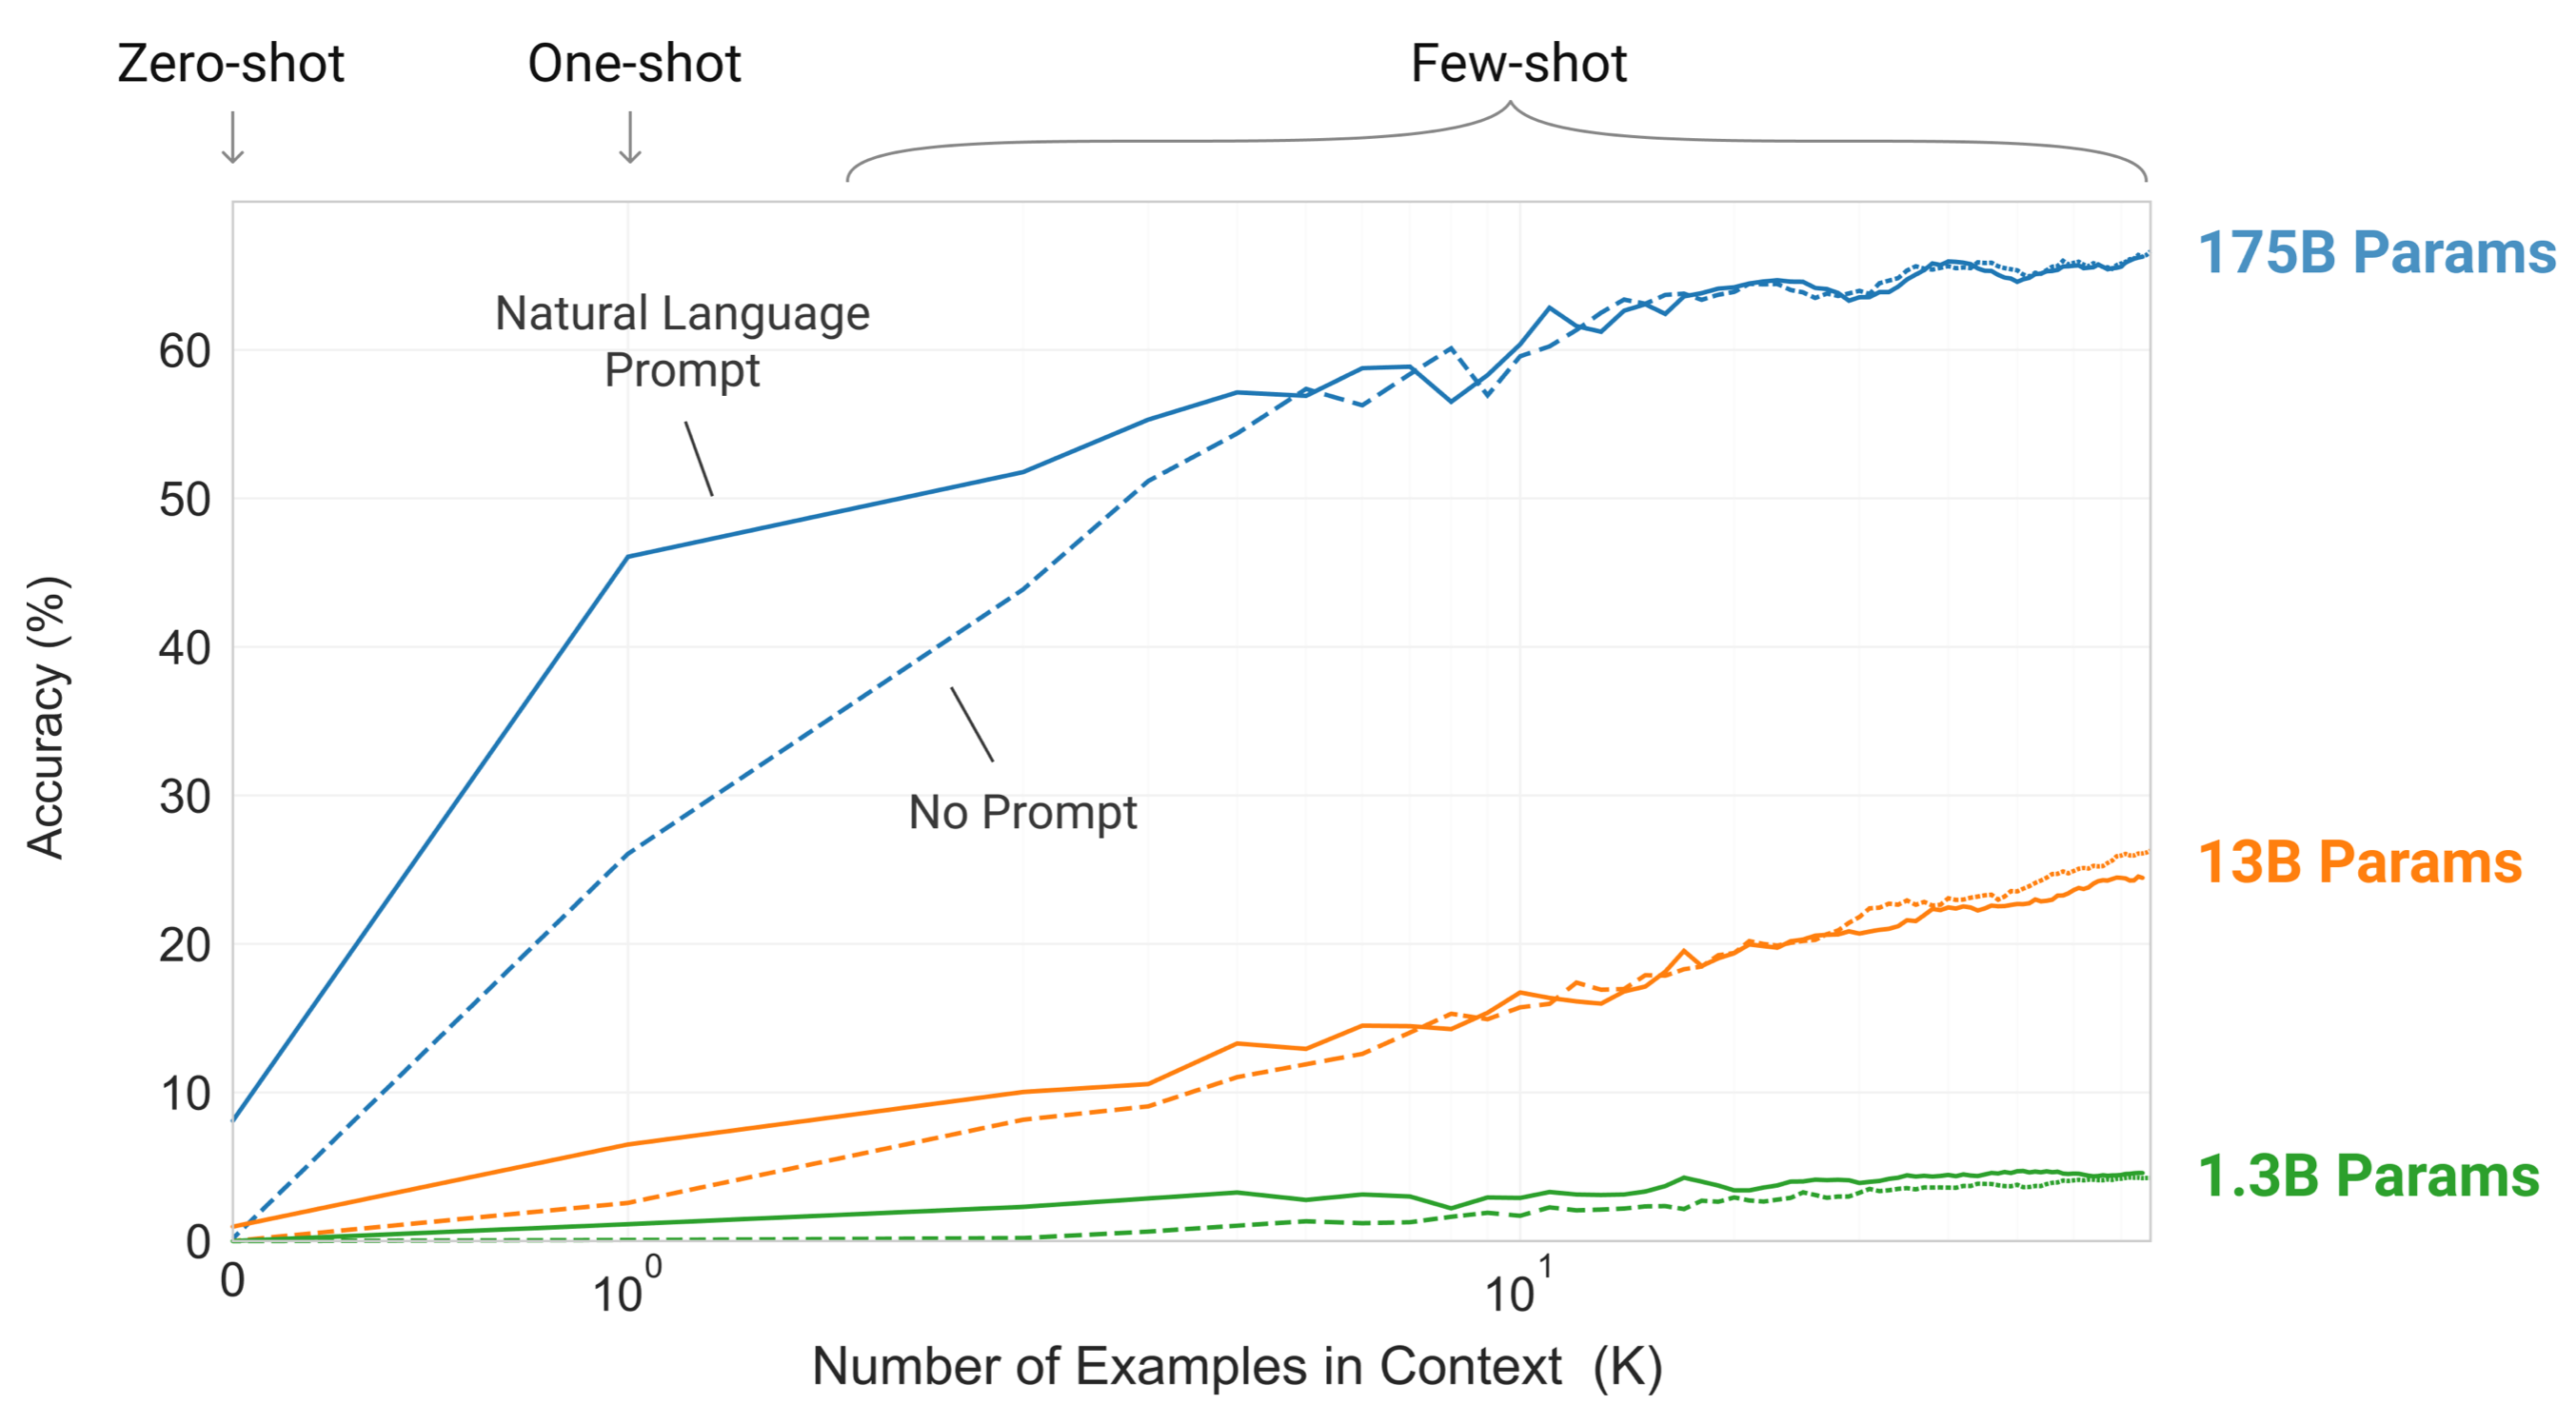
\includegraphics[width=8.50cm]{figure/incontextlearning.png}\\
		\citebutton{Source: Brown et al., 2020}{https://arxiv.org/abs/2005.14165}
\end{figure}

\begin{itemize}
	\item Number/Selection of demonstrations = Hyperparameter
	\item Larger model $\to$ Better in-context learning capabilities
\end{itemize}

\vfill

\scriptsize{*on an artificial, simple word scrambling/manipulation task}

\end{frame}

% ------------------------------------------------------------------------------

\begin{frame}{Architecture}

\vfill

\begin{itemize}
	\item Various sizes released; GPT-3 usually refers to largest one
	\item Both width ($d_{model}$) and depth ($n_{layers}$) are scaled
	\item Number of heads adjusted to $d_{model}$
\end{itemize}

	\begin{figure}
		\centering
		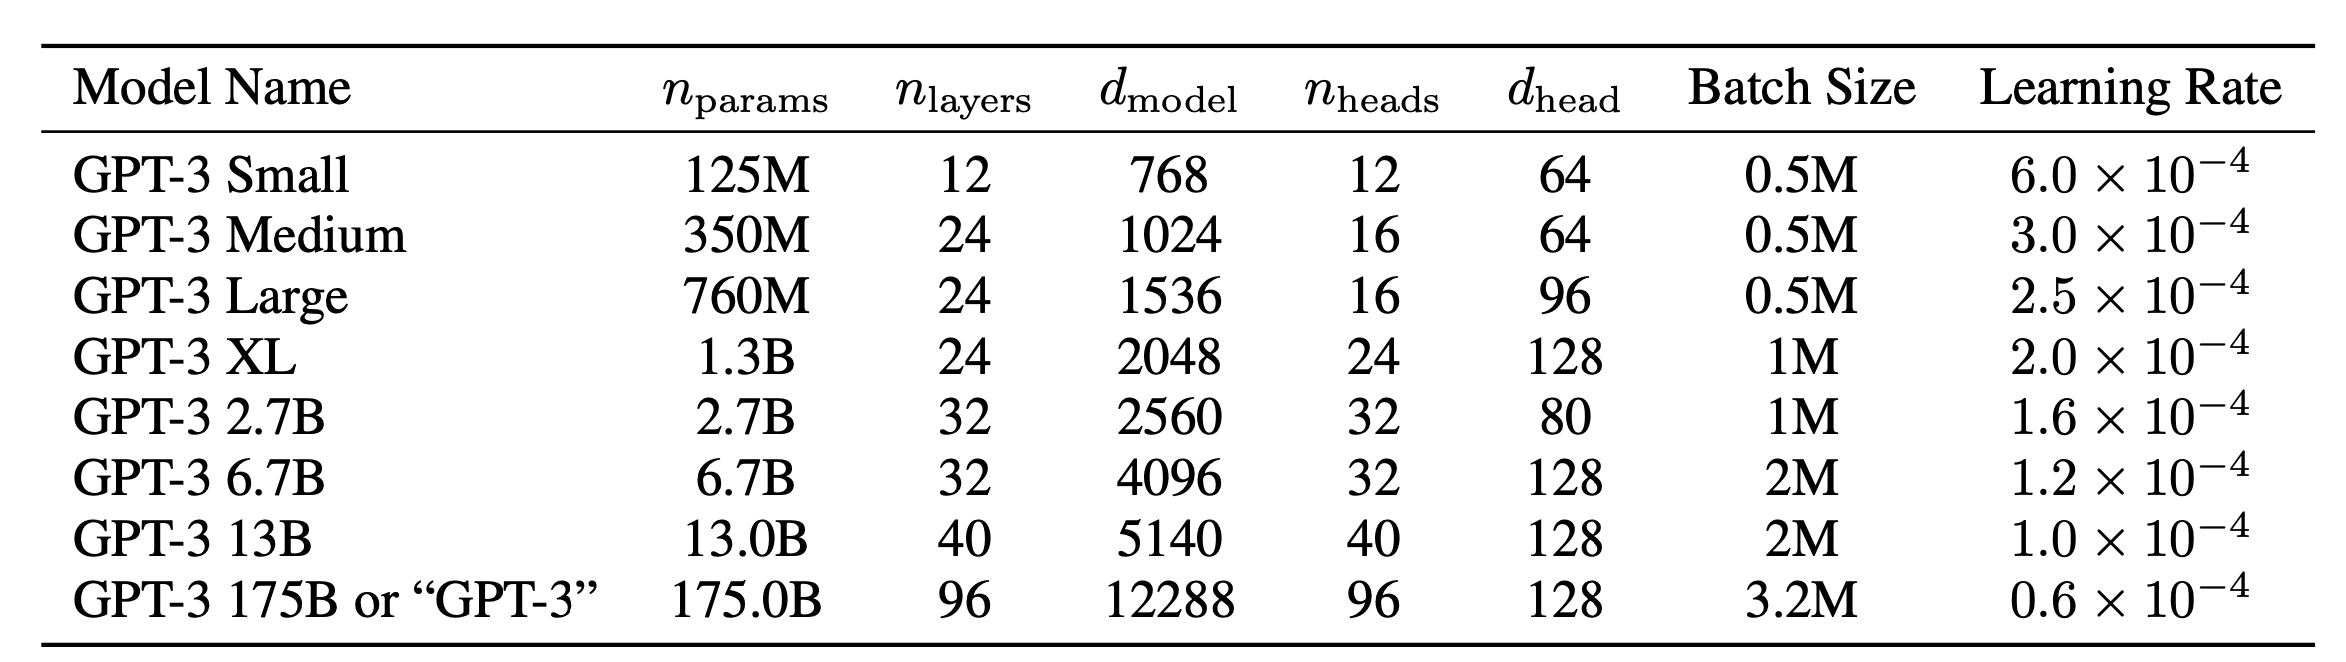
\includegraphics[width=11cm]{figure/gptarch.png}\\
		\citebutton{Source: Brown et al., 2020}{https://arxiv.org/abs/2005.14165}
	\end{figure}

\vfill

\end{frame}

% ------------------------------------------------------------------------------

\begin{frame}{Training corpus}

\vfill

\begin{itemize}
	\item BERT: 3.3B words (rougly 4B -- 6B tokens)
	\item GPT-3: 499B tokens
	\item Increased by two orders of magnitude within < 2yrs
	\item Content: Mostly the internet (incl. test sets of popular benchmarks)
\end{itemize}

	\begin{figure}
		\centering
		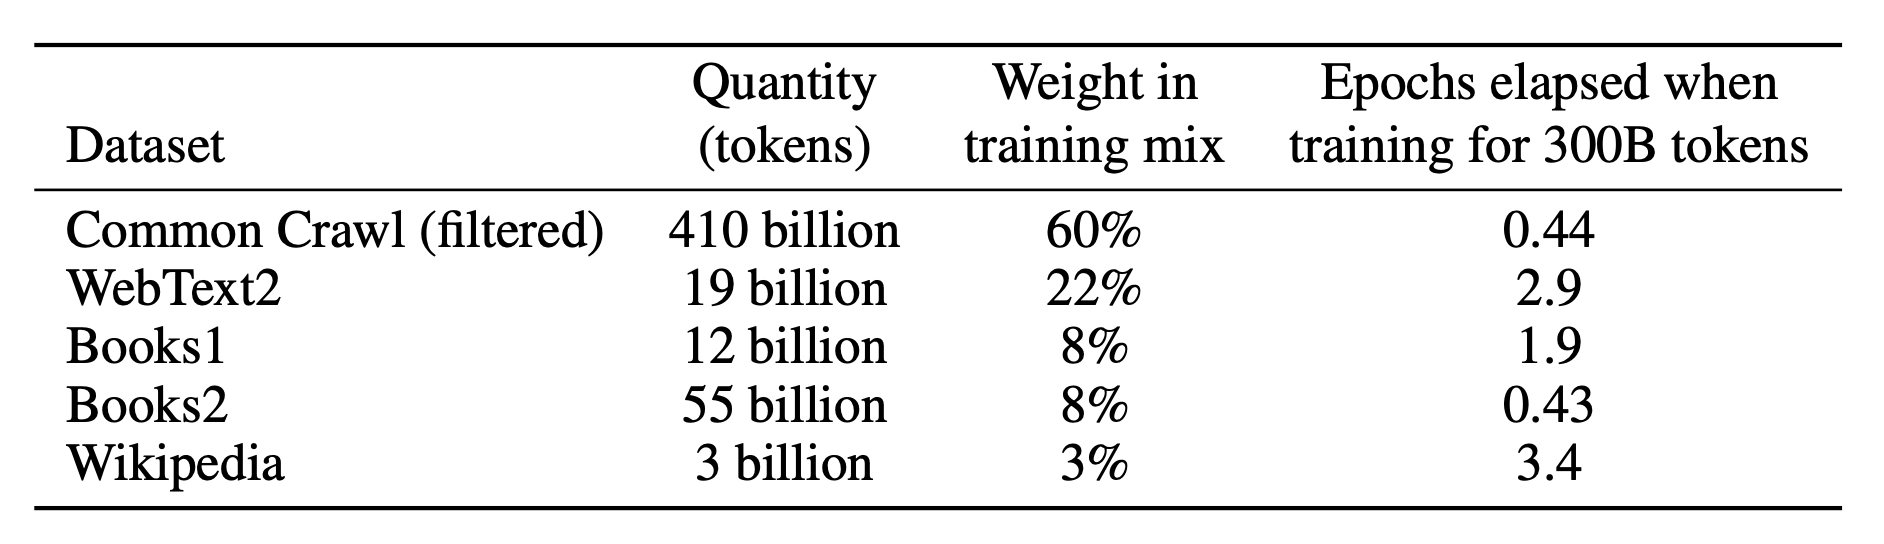
\includegraphics[width=11cm]{figure/traincorp.png}\\
		\citebutton{Source: Brown et al., 2020}{https://arxiv.org/abs/2005.14165}
	\end{figure}
\vfill

\end{frame}

% ------------------------------------------------------------------------------

\begin{frame}{X-shot comparison}
	
	\vfill
	
\begin{itemize}
	\item 42 accuracy-denominated benchmarks
	\item Few-shot performance increases faster than zero-shot
\end{itemize}

	\begin{figure}
		\centering
		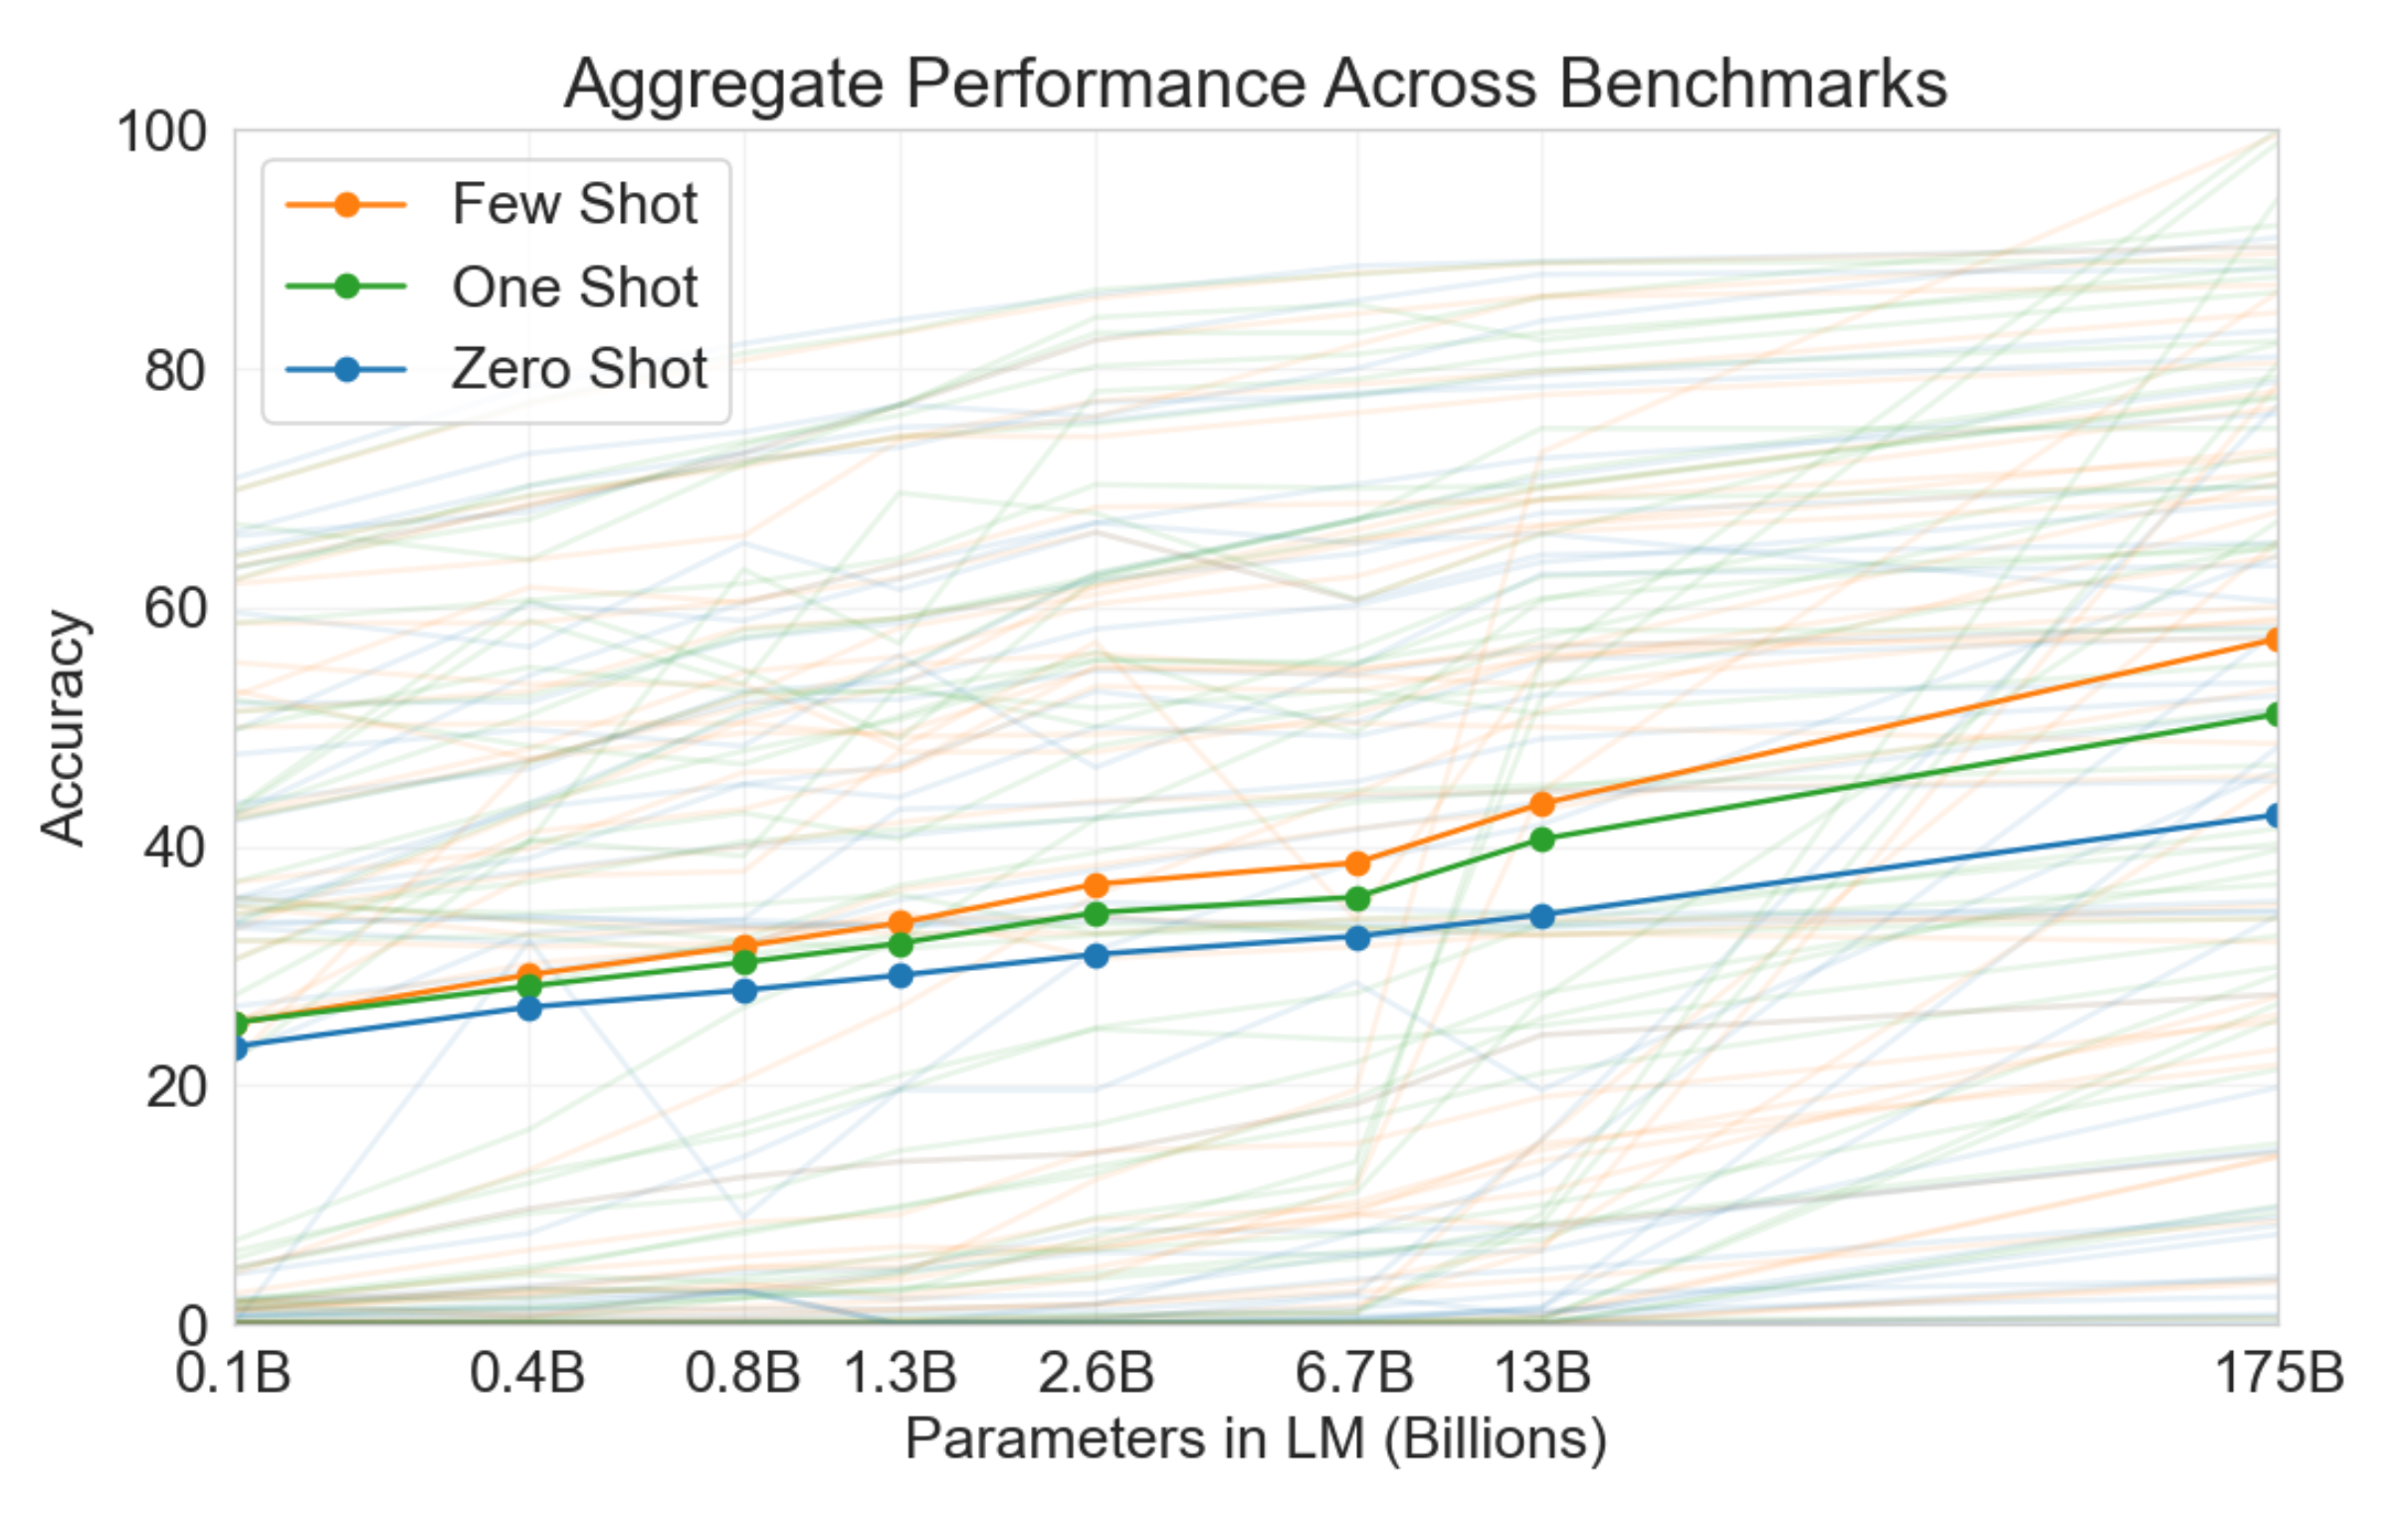
\includegraphics[width=7.65cm]{figure/xshotlargecorpora.png}\\
		\citebutton{Source: Brown et al., 2020}{https://arxiv.org/abs/2005.14165}
	\end{figure}
	
	\vfill
	
\end{frame}

% ------------------------------------------------------------------------------

\begin{frame}{Loss as a function of compute}

\vfill

\textbf{Power-law trend}

	\begin{figure}
		\centering
		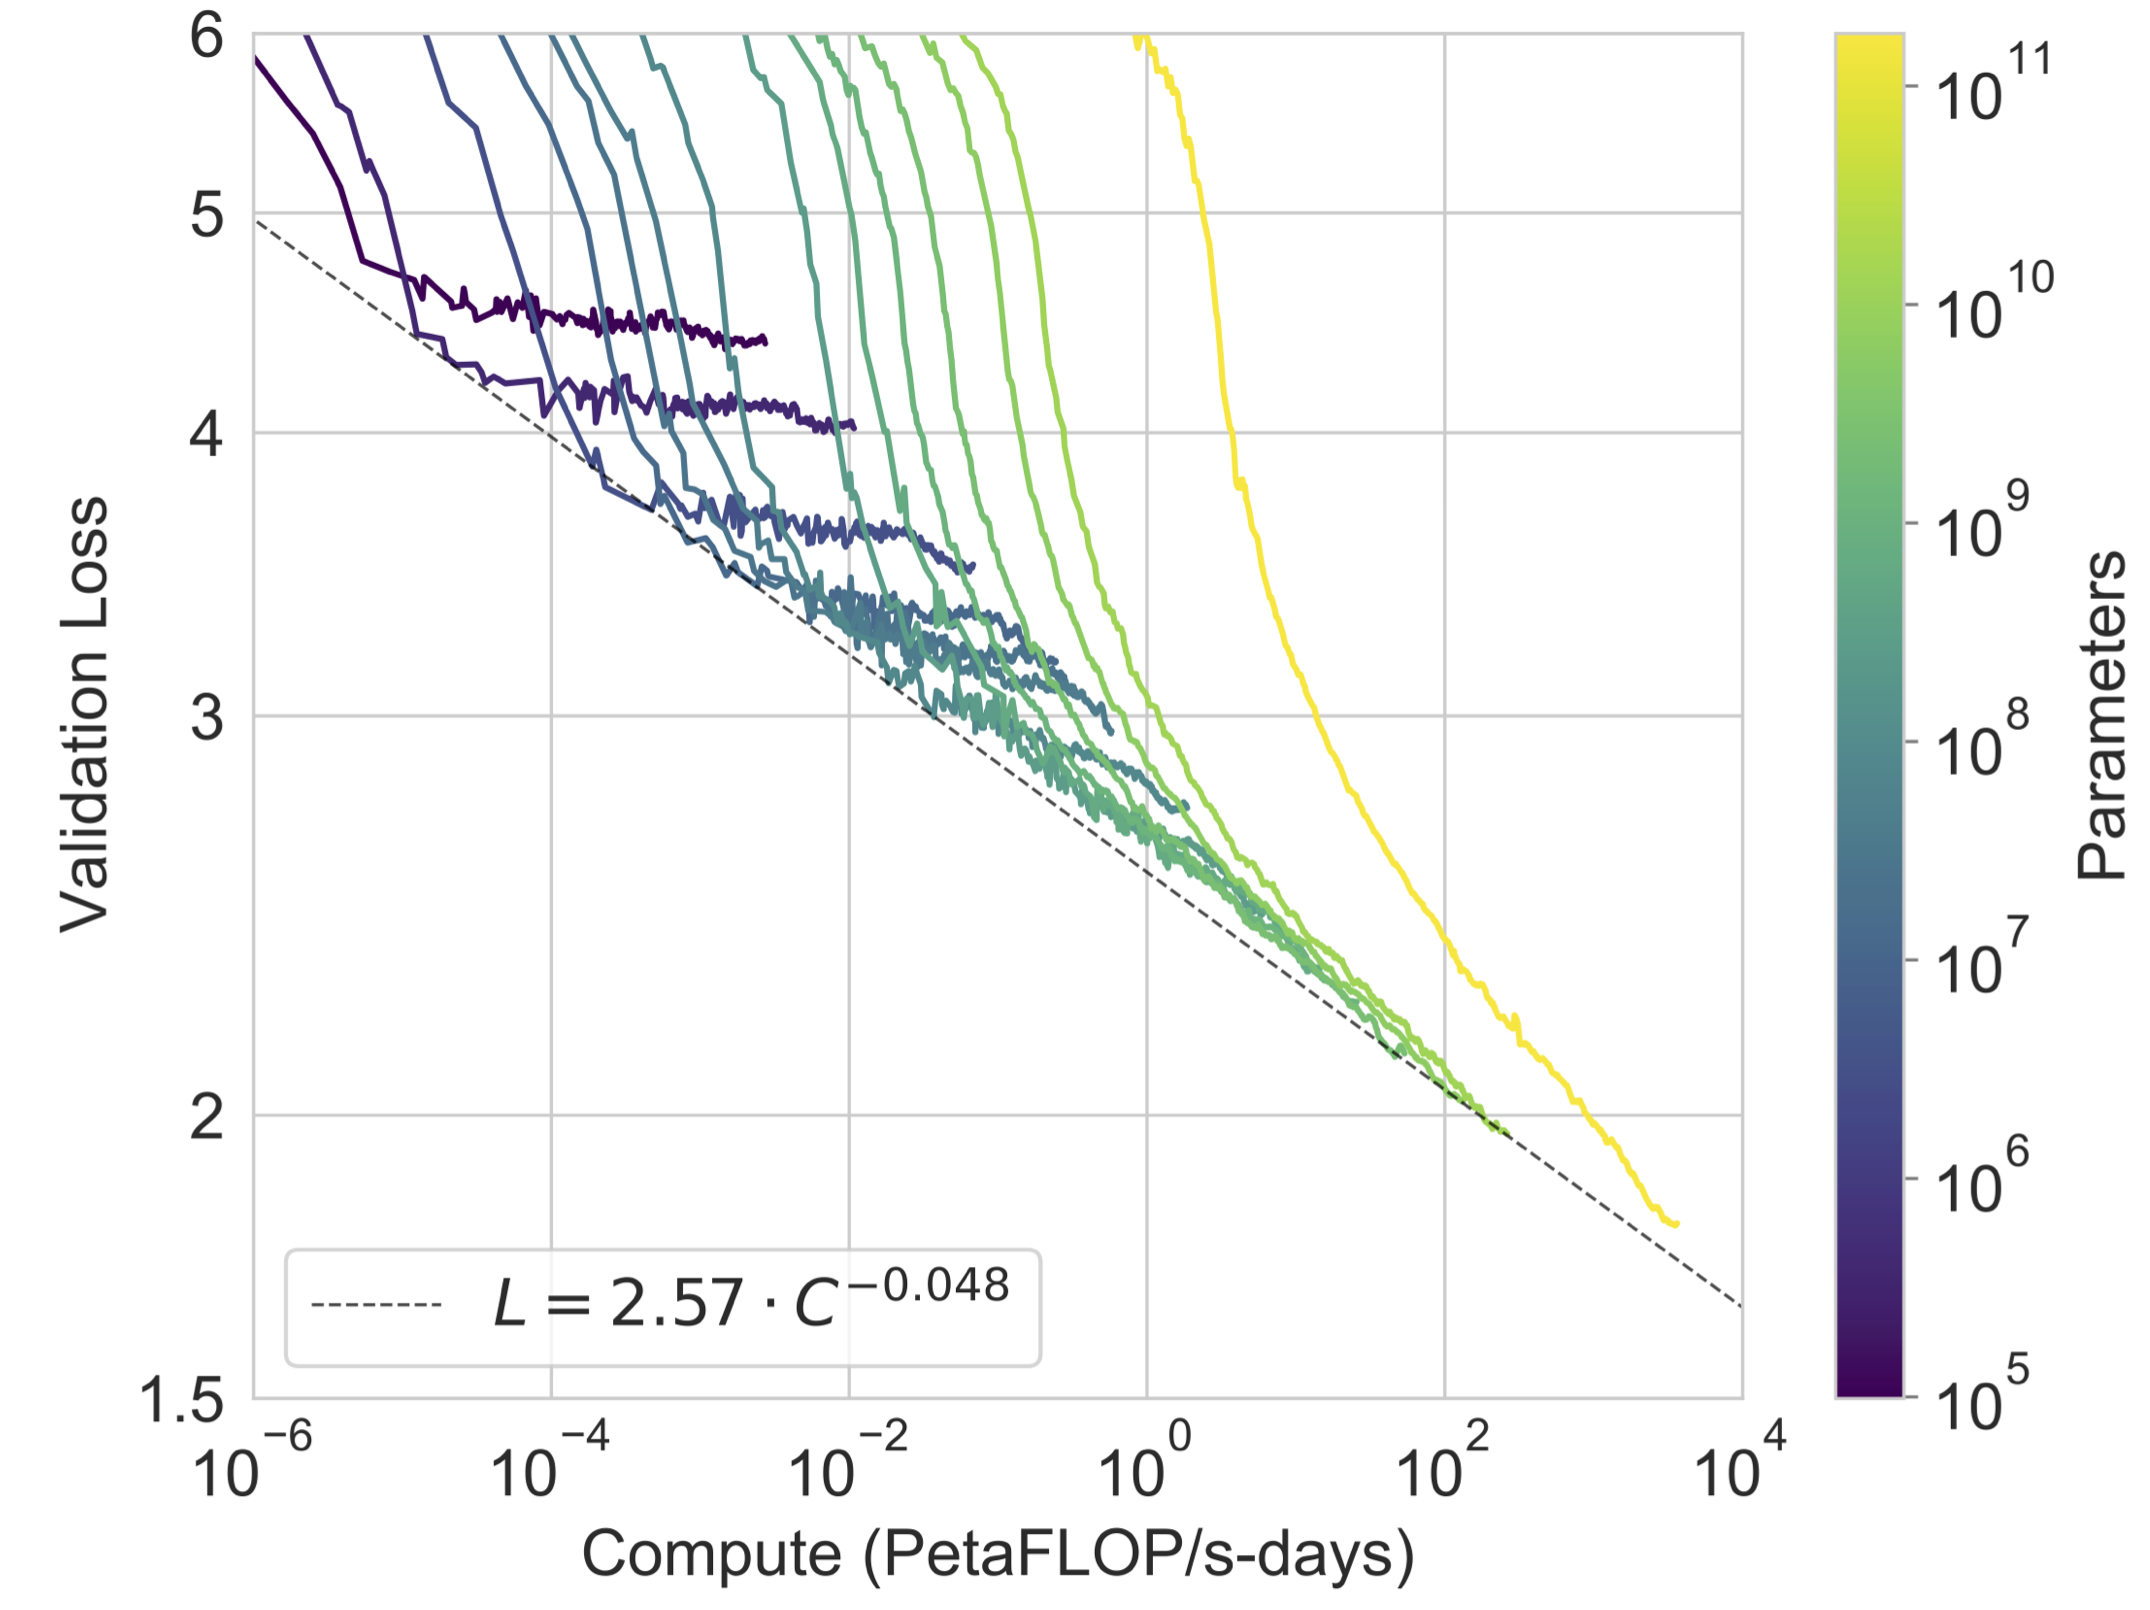
\includegraphics[width=8cm]{figure/losscompute.png}\\
		\citebutton{Source: Brown et al., 2020}{https://arxiv.org/abs/2005.14165}
	\end{figure}

\vfill

\end{frame}

% ------------------------------------------------------------------------------


%%%%%%%%%%%%%%%%%%%%%%%%%%%%%%%%%%%%%%%%%%%%%%%%%%%%%%%%%%%%%%%%%%
\section{GPT-3: Tasks \& Performance}
% Source: DL4NLP chapter07-gpt/slides-74-tasks.tex
%%%%%%%%%%%%%%%%%%%%%%%%%%%%%%%%%%%%%%%%%%%%%%%%%%%%%%%%%%%%%%%%%%
% ------------------------------------------------------------------------------

\begin{frame}{Lambada task}

\vfill

	\begin{figure}
		\centering
		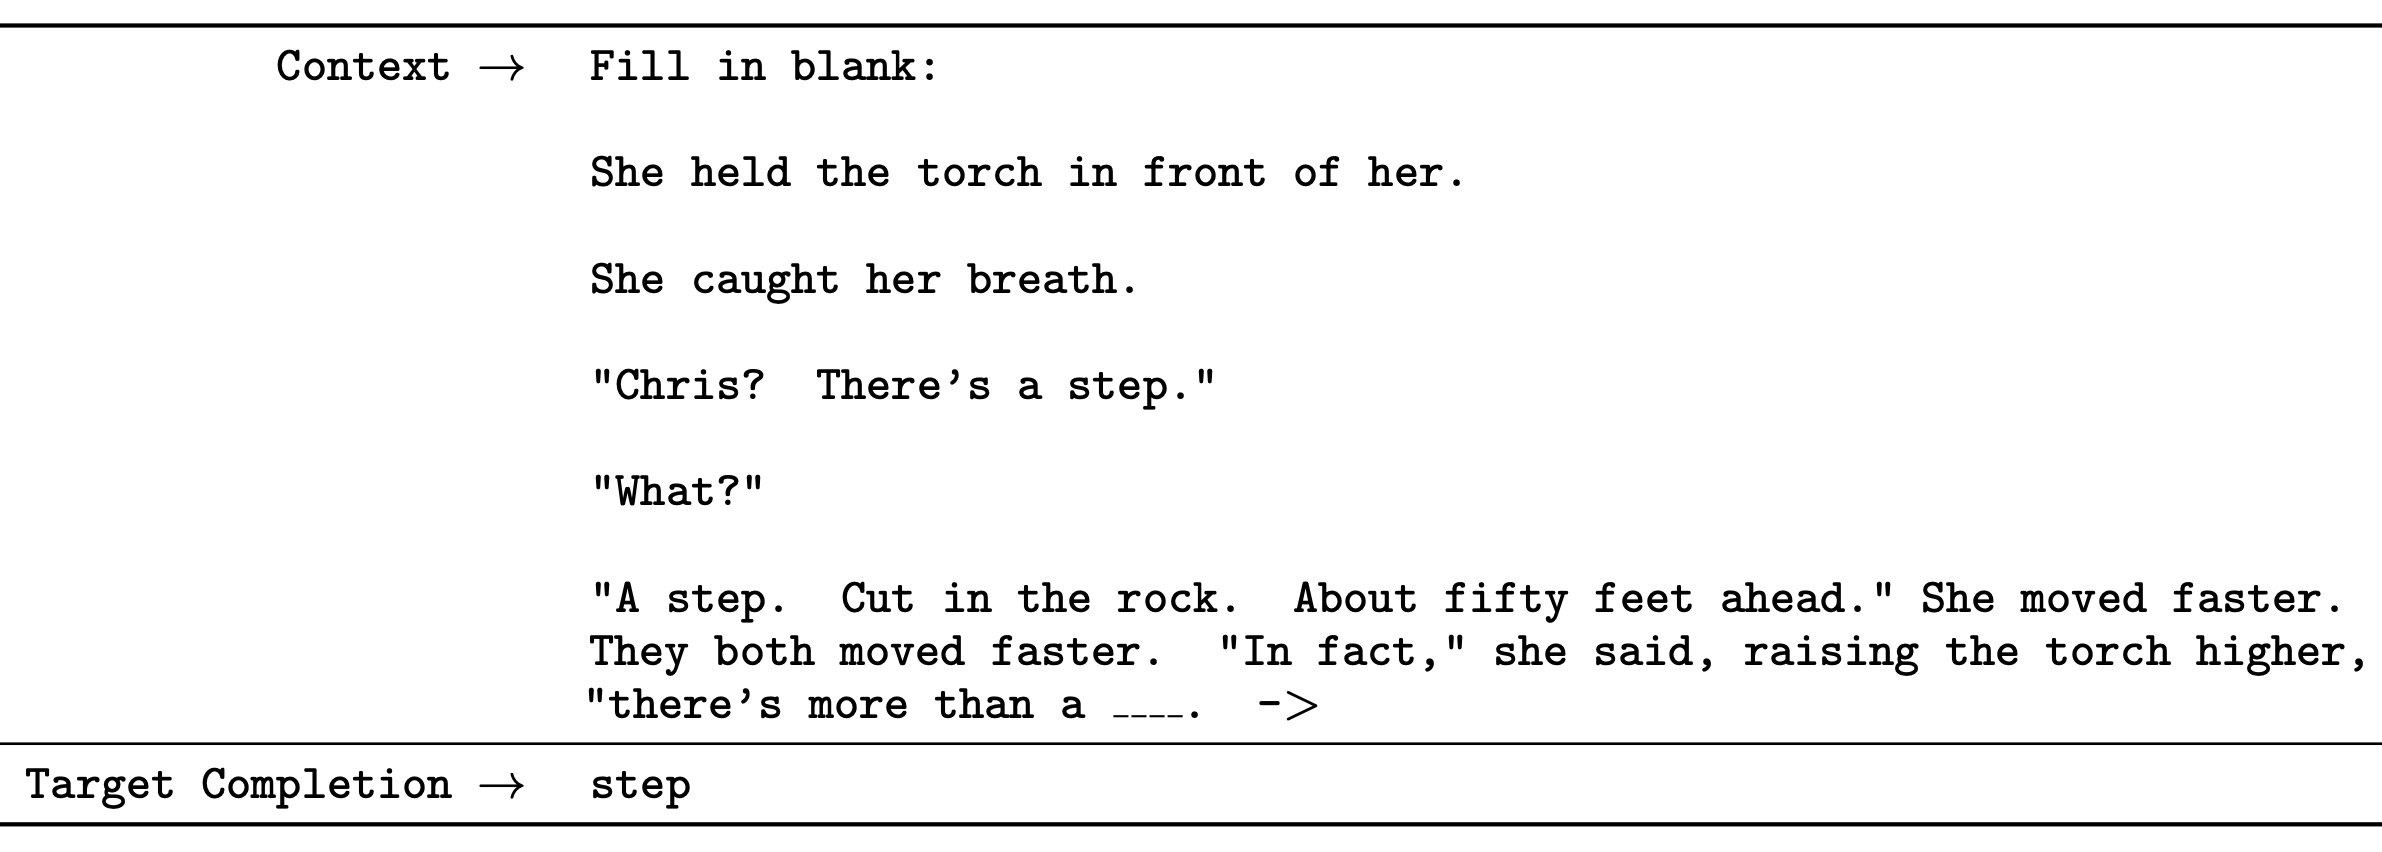
\includegraphics[width=10cm]{figure/lambadaformat.png}\\
		\citebutton{Source: Brown et al., 2020}{https://arxiv.org/abs/2005.14165}
	\end{figure}

\vfill

\end{frame}

% ------------------------------------------------------------------------------

\begin{frame}{Performance on lambada}

\vfill

	\begin{figure}
		\centering
		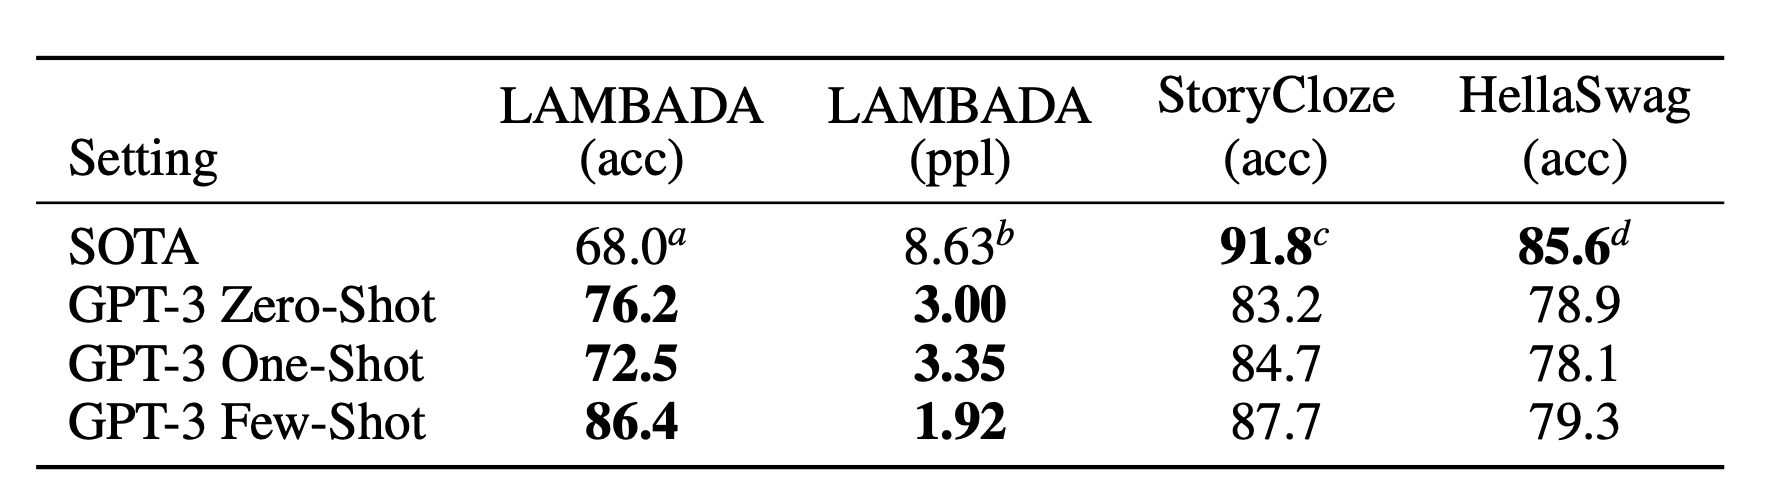
\includegraphics[width=10cm]{figure/lambadaperf.png}\\
		\citebutton{Source: Brown et al., 2020}{https://arxiv.org/abs/2005.14165}
	\end{figure}

\vfill

\end{frame}

% ------------------------------------------------------------------------------

\begin{frame}{``Closed book'' question answering (QA)}

\vfill
			
	\begin{figure}
		\centering
		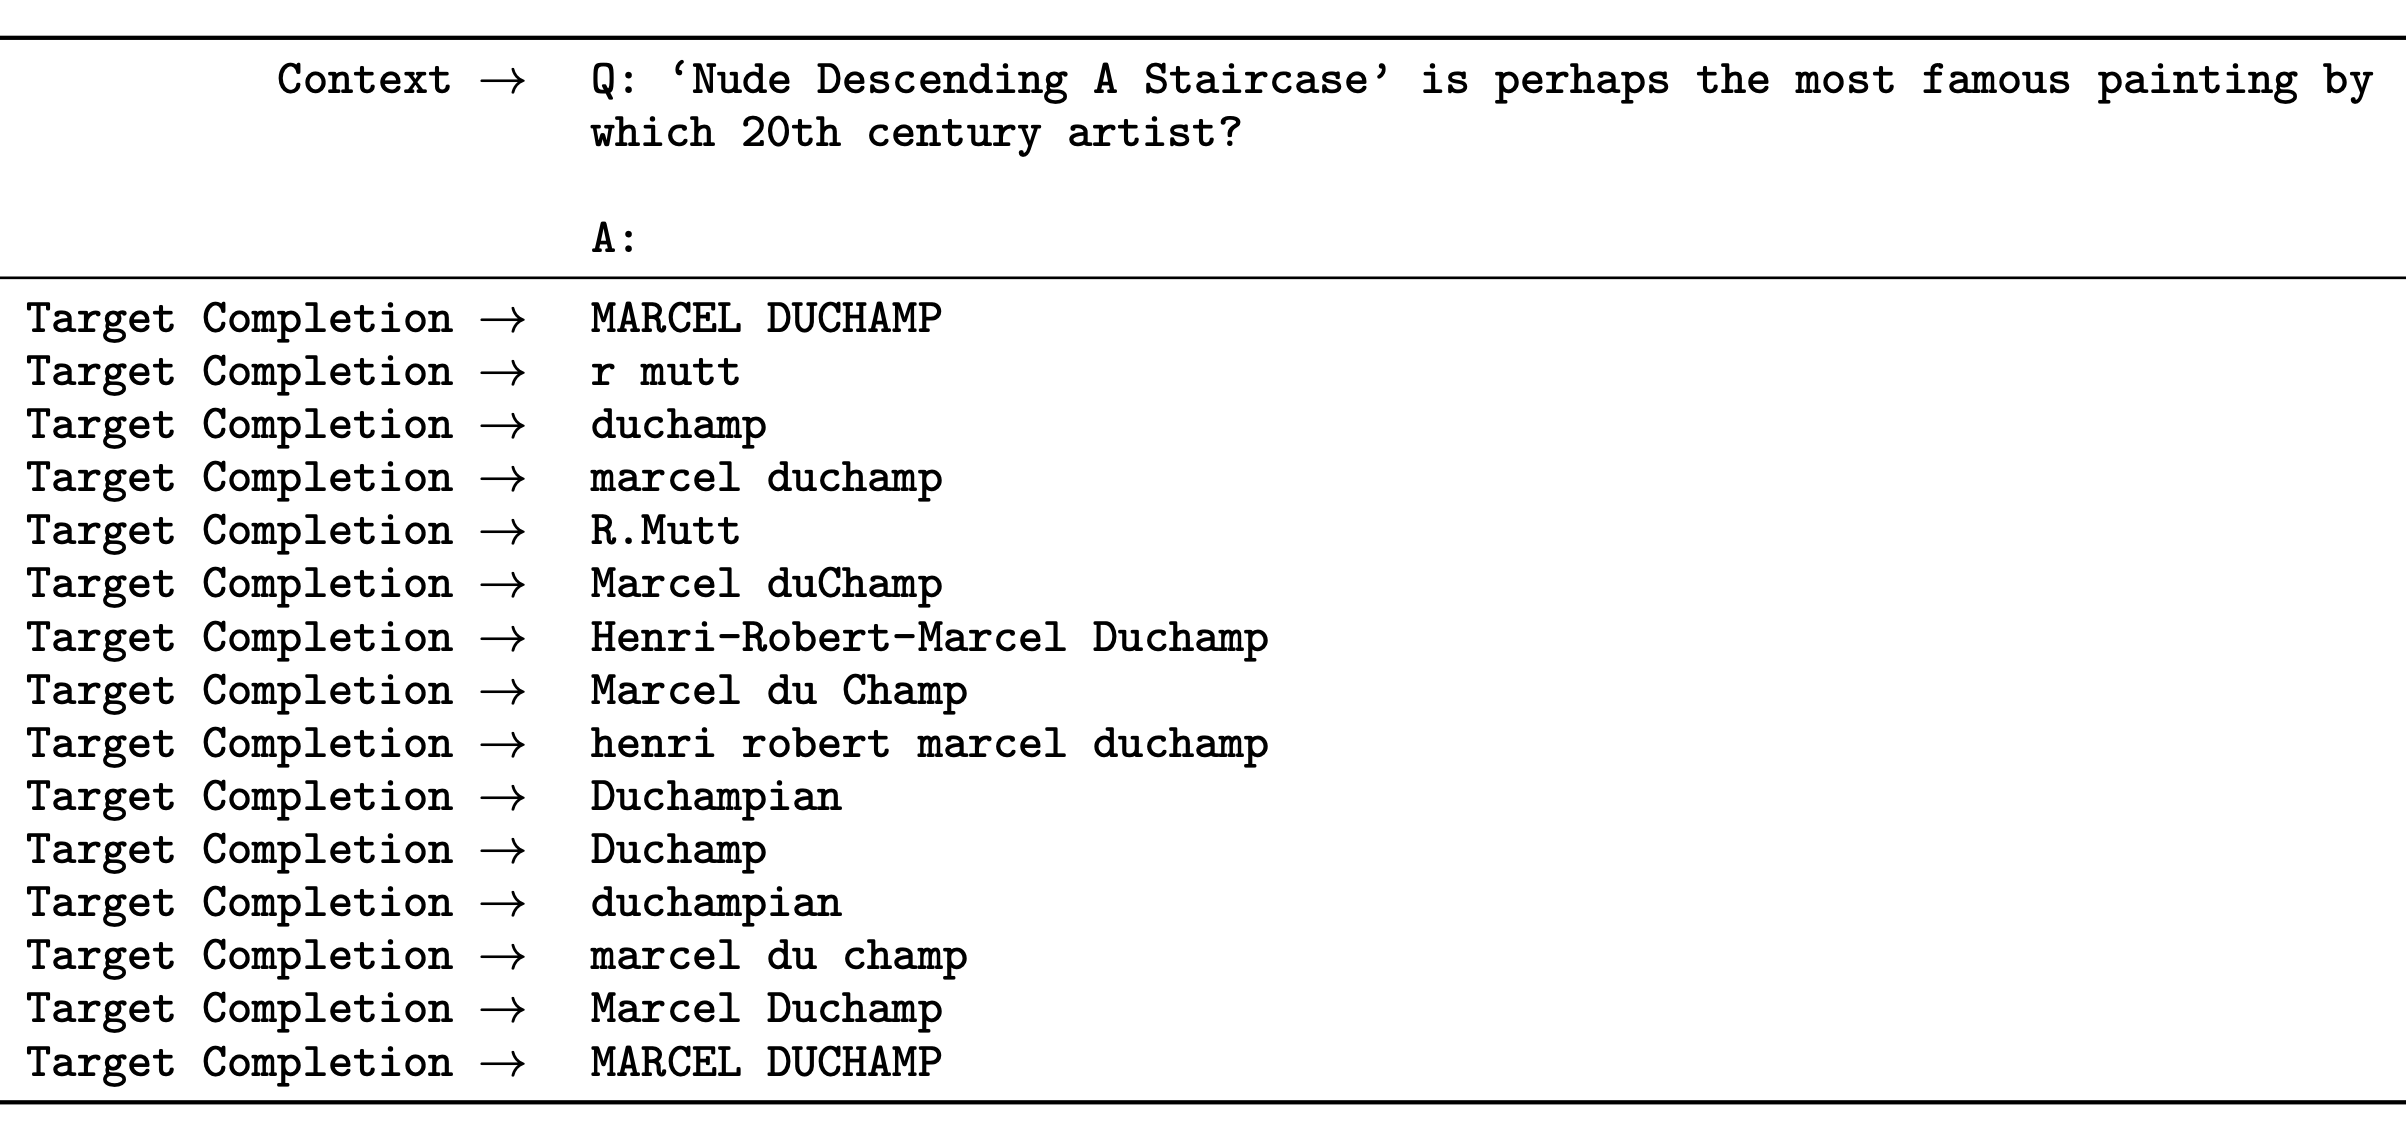
\includegraphics[width=10cm]{figure/triviaformat.png}\\
		\citebutton{Source: Brown et al., 2020}{https://arxiv.org/abs/2005.14165}
	\end{figure}
	
\vfill

\end{frame}

% ------------------------------------------------------------------------------

\begin{frame}{Performance on the closed-book QA}

\vfill

	\begin{figure}
		\centering
		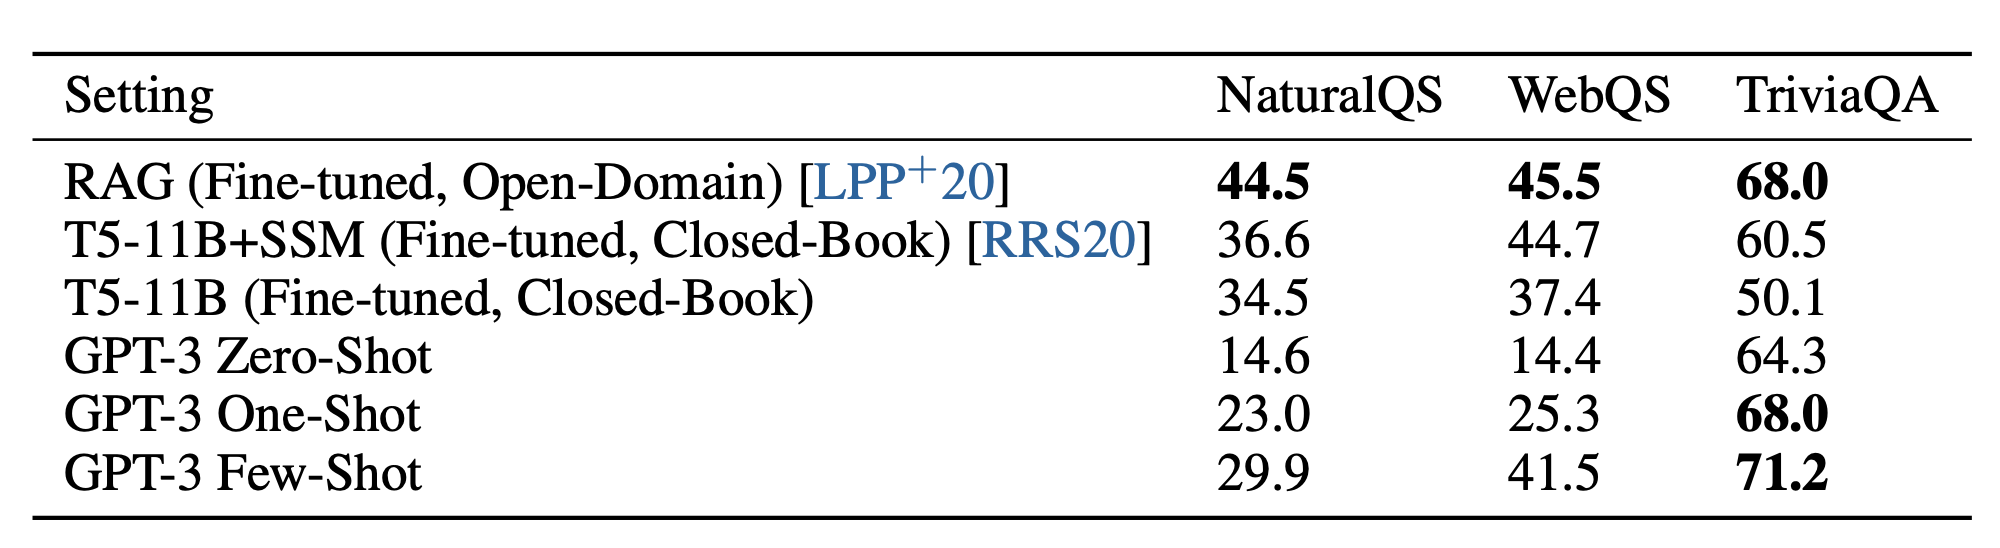
\includegraphics[width=10cm]{figure/triviaperf.png}\\
		\citebutton{Source: Brown et al., 2020}{https://arxiv.org/abs/2005.14165}
	\end{figure}

\vfill

\end{frame}

% ------------------------------------------------------------------------------

\begin{frame}{Performance on machine translation}

\vfill

	\begin{figure}
		\centering
		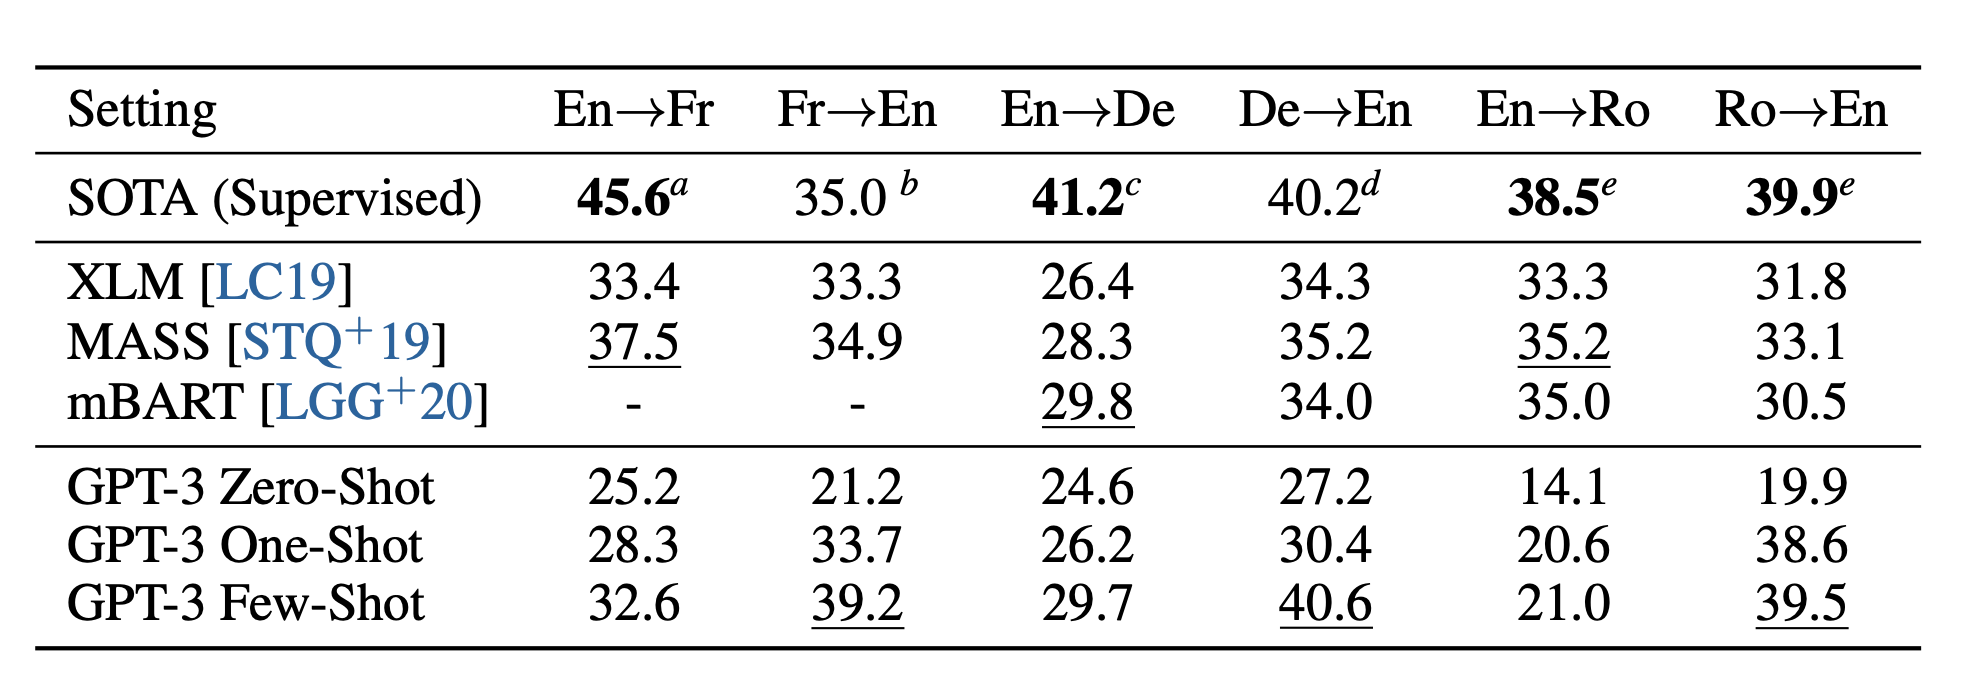
\includegraphics[width=10cm]{figure/mtperf.png}\\
		\citebutton{Source: Brown et al., 2020}{https://arxiv.org/abs/2005.14165}
	\end{figure}

\vfill

\end{frame}

% ------------------------------------------------------------------------------

\begin{frame}{Winograd task}

\vfill

	\begin{figure}
		\centering
		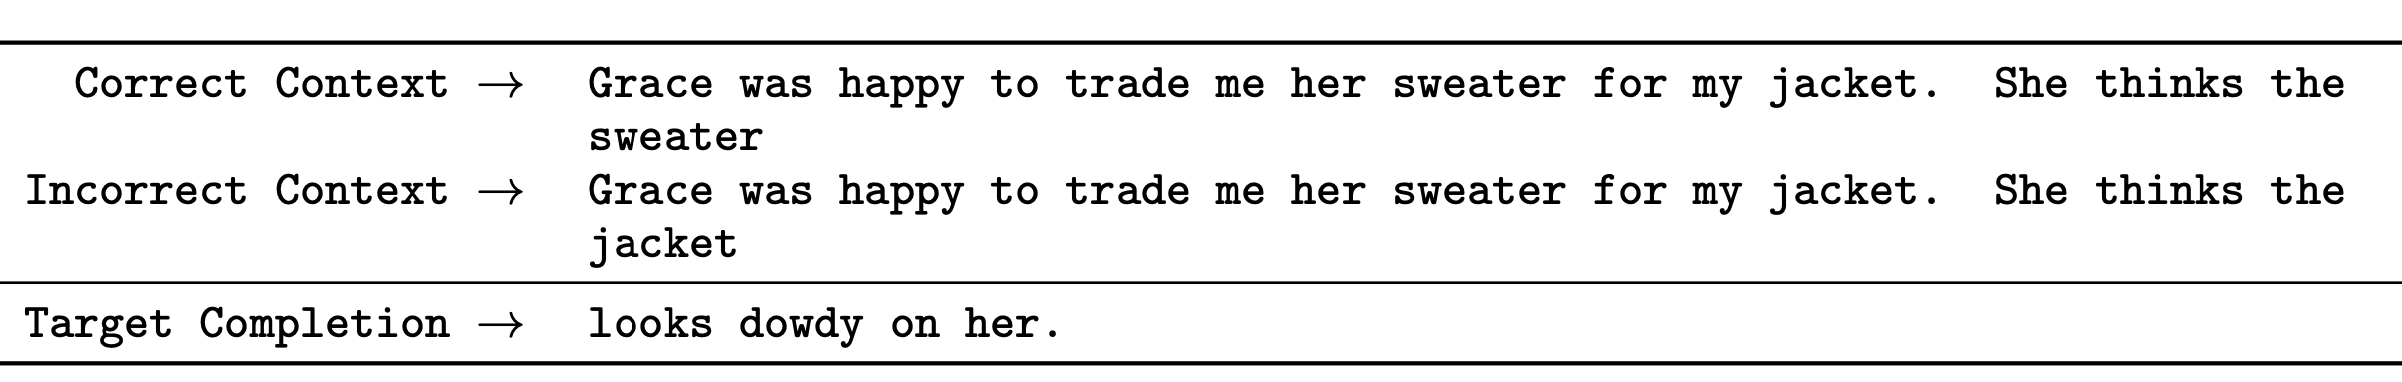
\includegraphics[width=10cm]{figure/winogradformat.png}\\
		\citebutton{Source: Brown et al., 2020}{https://arxiv.org/abs/2005.14165}
	\end{figure}

\vfill

\end{frame}


% ------------------------------------------------------------------------------

\begin{frame}{Performance on Winograd task}

\vfill

	\begin{figure}
		\centering
		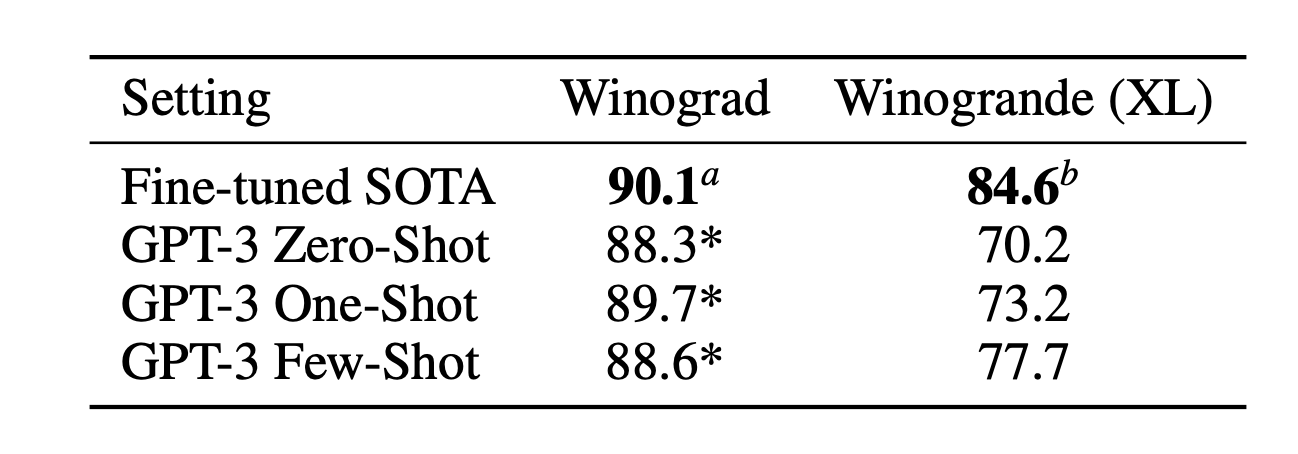
\includegraphics[width=10cm]{figure/winogradperf.png}\\
		\citebutton{Source: Brown et al., 2020}{https://arxiv.org/abs/2005.14165}
	\end{figure}

\vfill

\end{frame}


% ------------------------------------------------------------------------------

\begin{frame}{ARC task}

\vfill

\begin{itemize}
	\item Multipe-Choice questions from 3rd to 9th grad science exams
	\item \textit{Challenge} version: Filtered to questions that simple statistical or information retrieval methods are unable to correctly answer
\end{itemize}

	\begin{figure}
		\centering
		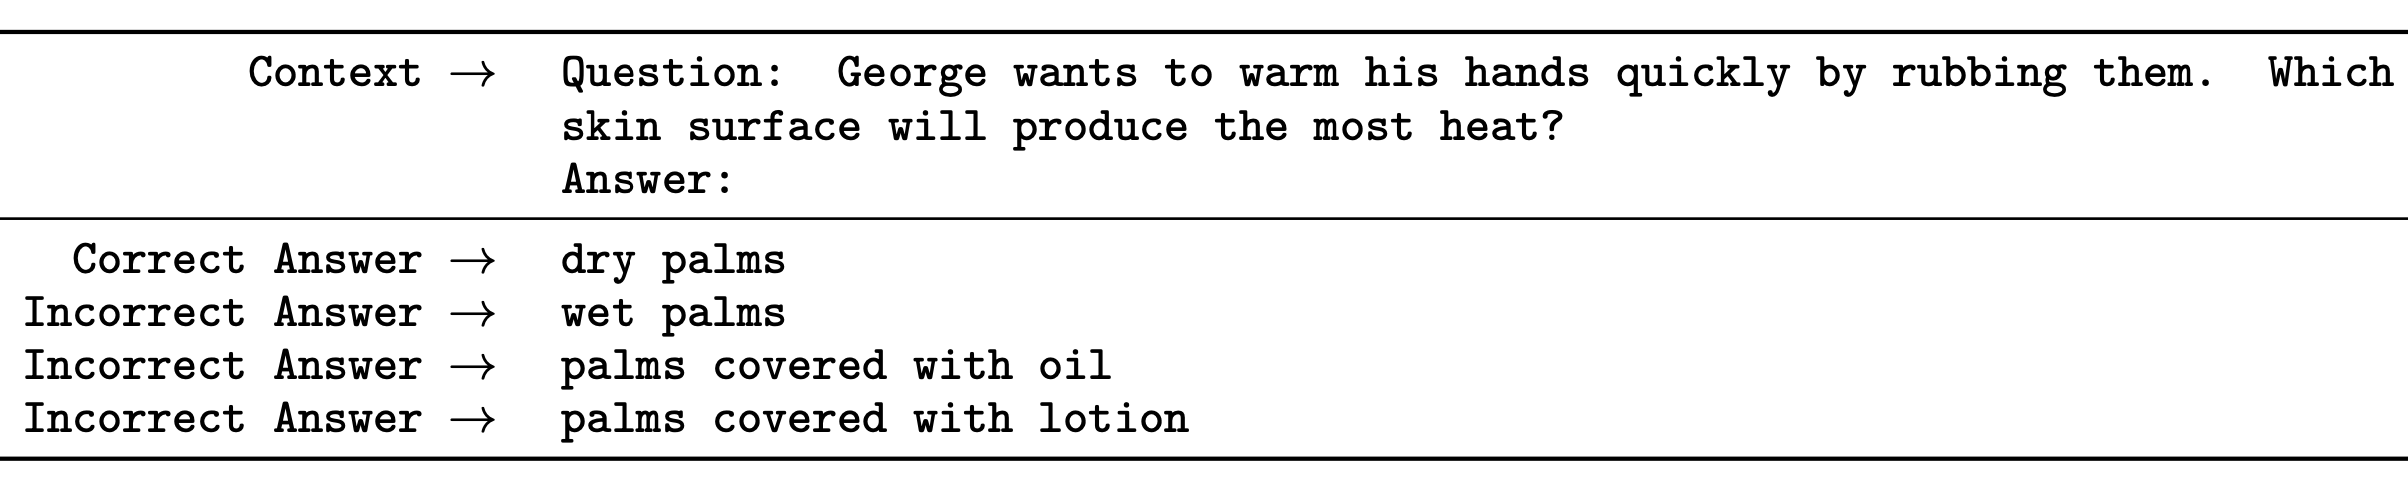
\includegraphics[width=10cm]{figure/arcformat.png}\\
		\citebutton{Source: Brown et al., 2020}{https://arxiv.org/abs/2005.14165}
	\end{figure}

\vfill

\end{frame}


% ------------------------------------------------------------------------------

\begin{frame}{Performance on ARC task}

\vfill

	\begin{figure}
		\centering
		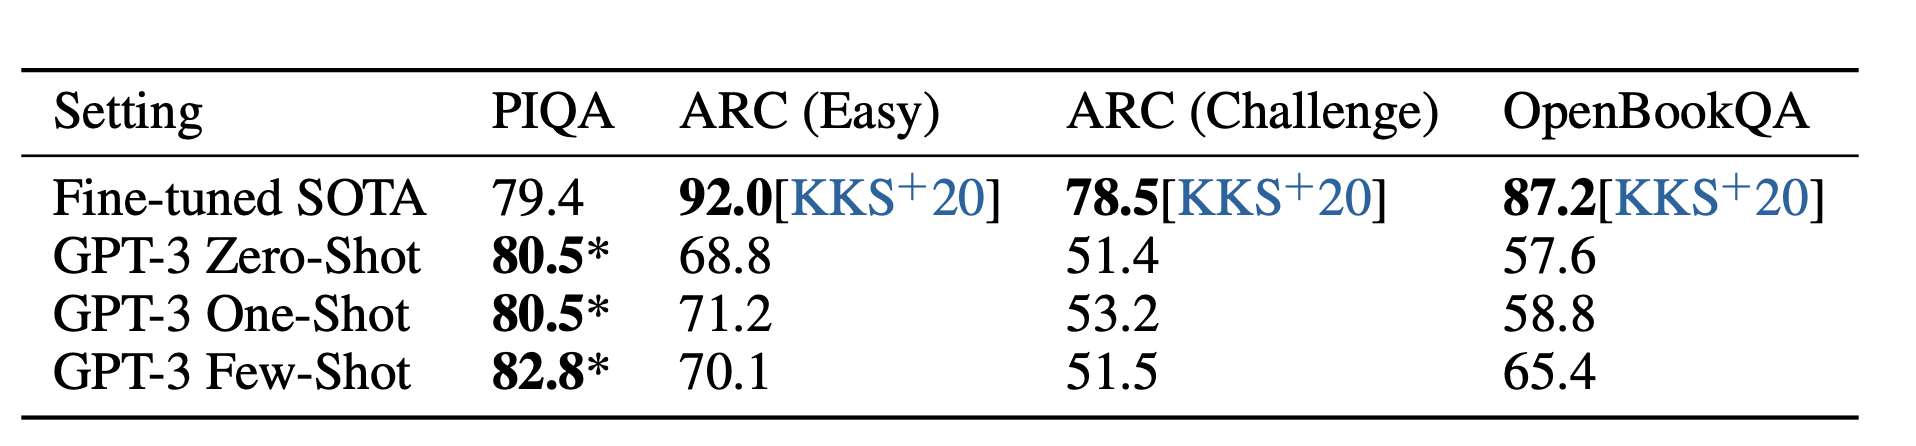
\includegraphics[width=10cm]{figure/arcperf.png}
	\end{figure}

\vfill

\end{frame}


% ------------------------------------------------------------------------------

\begin{frame}{RACE task}

\vfill

	\begin{figure}
		\centering
		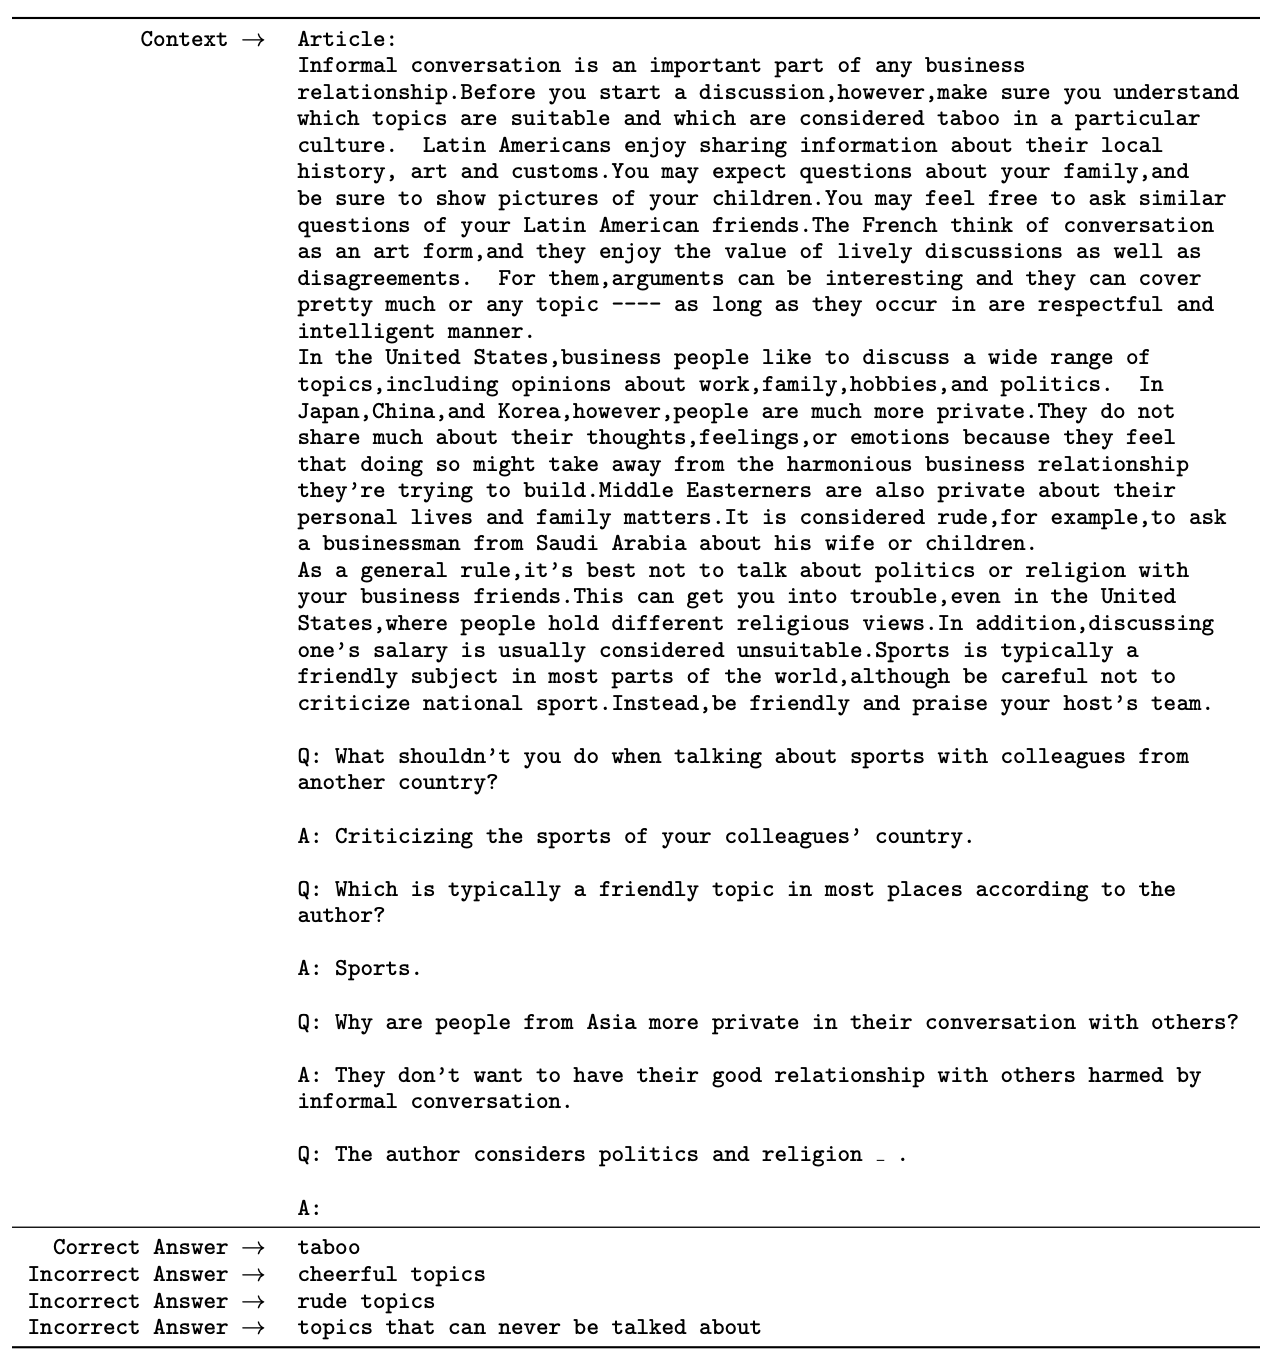
\includegraphics[width=5.78cm]{figure/raceformat,h.png}
	\end{figure}
	
\vfill

\end{frame}



% ------------------------------------------------------------------------------

\begin{frame}{Performance on RACE task}

\vfill

	\begin{figure}
		\centering
		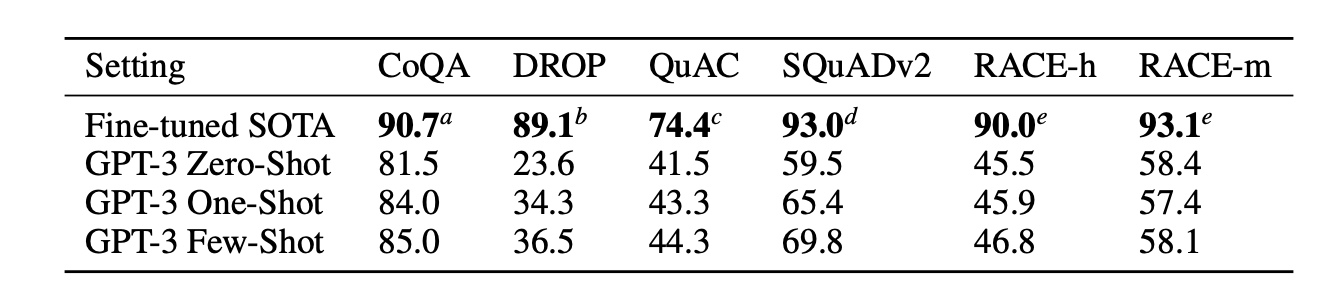
\includegraphics[width=10cm]{figure/raceperf.png}
	\end{figure}

\vfill

\end{frame}



% ------------------------------------------------------------------------------

\begin{frame}{Performance on SuperGLUE task}

\vfill

	\begin{figure}
		\centering
		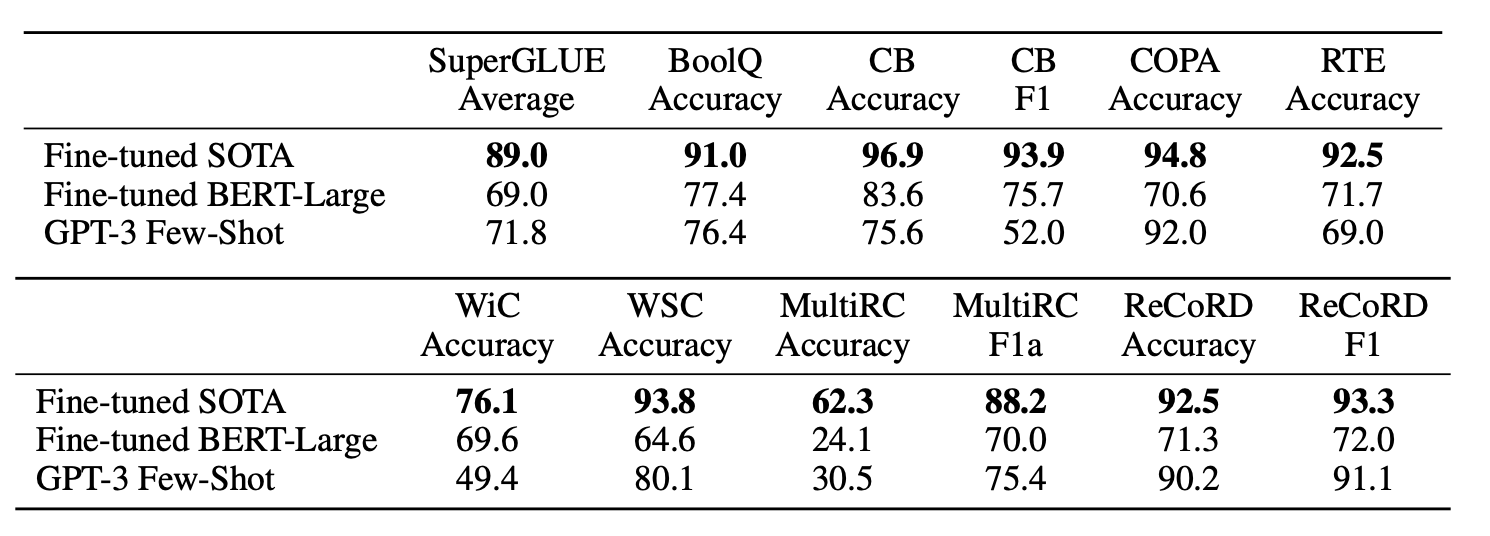
\includegraphics[width=10cm]{figure/superglueperf.png}
	\end{figure}

\vfill

\end{frame}



% ------------------------------------------------------------------------------

\begin{frame}{SuperGLUE}

\vfill

  \begin{itemize}
\item BoolQ
\item CB (true/false/neither)
\item COPA
\item RTE (similar to natural language inference)
\item WiC 
\item WSC
\item MultiRC (true/false)
\item ReCoRD 
    \end{itemize}

\vfill

\end{frame}



% ------------------------------------------------------------------------------

\begin{frame}{BoolQ (Boolean Question) task}

\vfill

	\begin{figure}
		\centering
		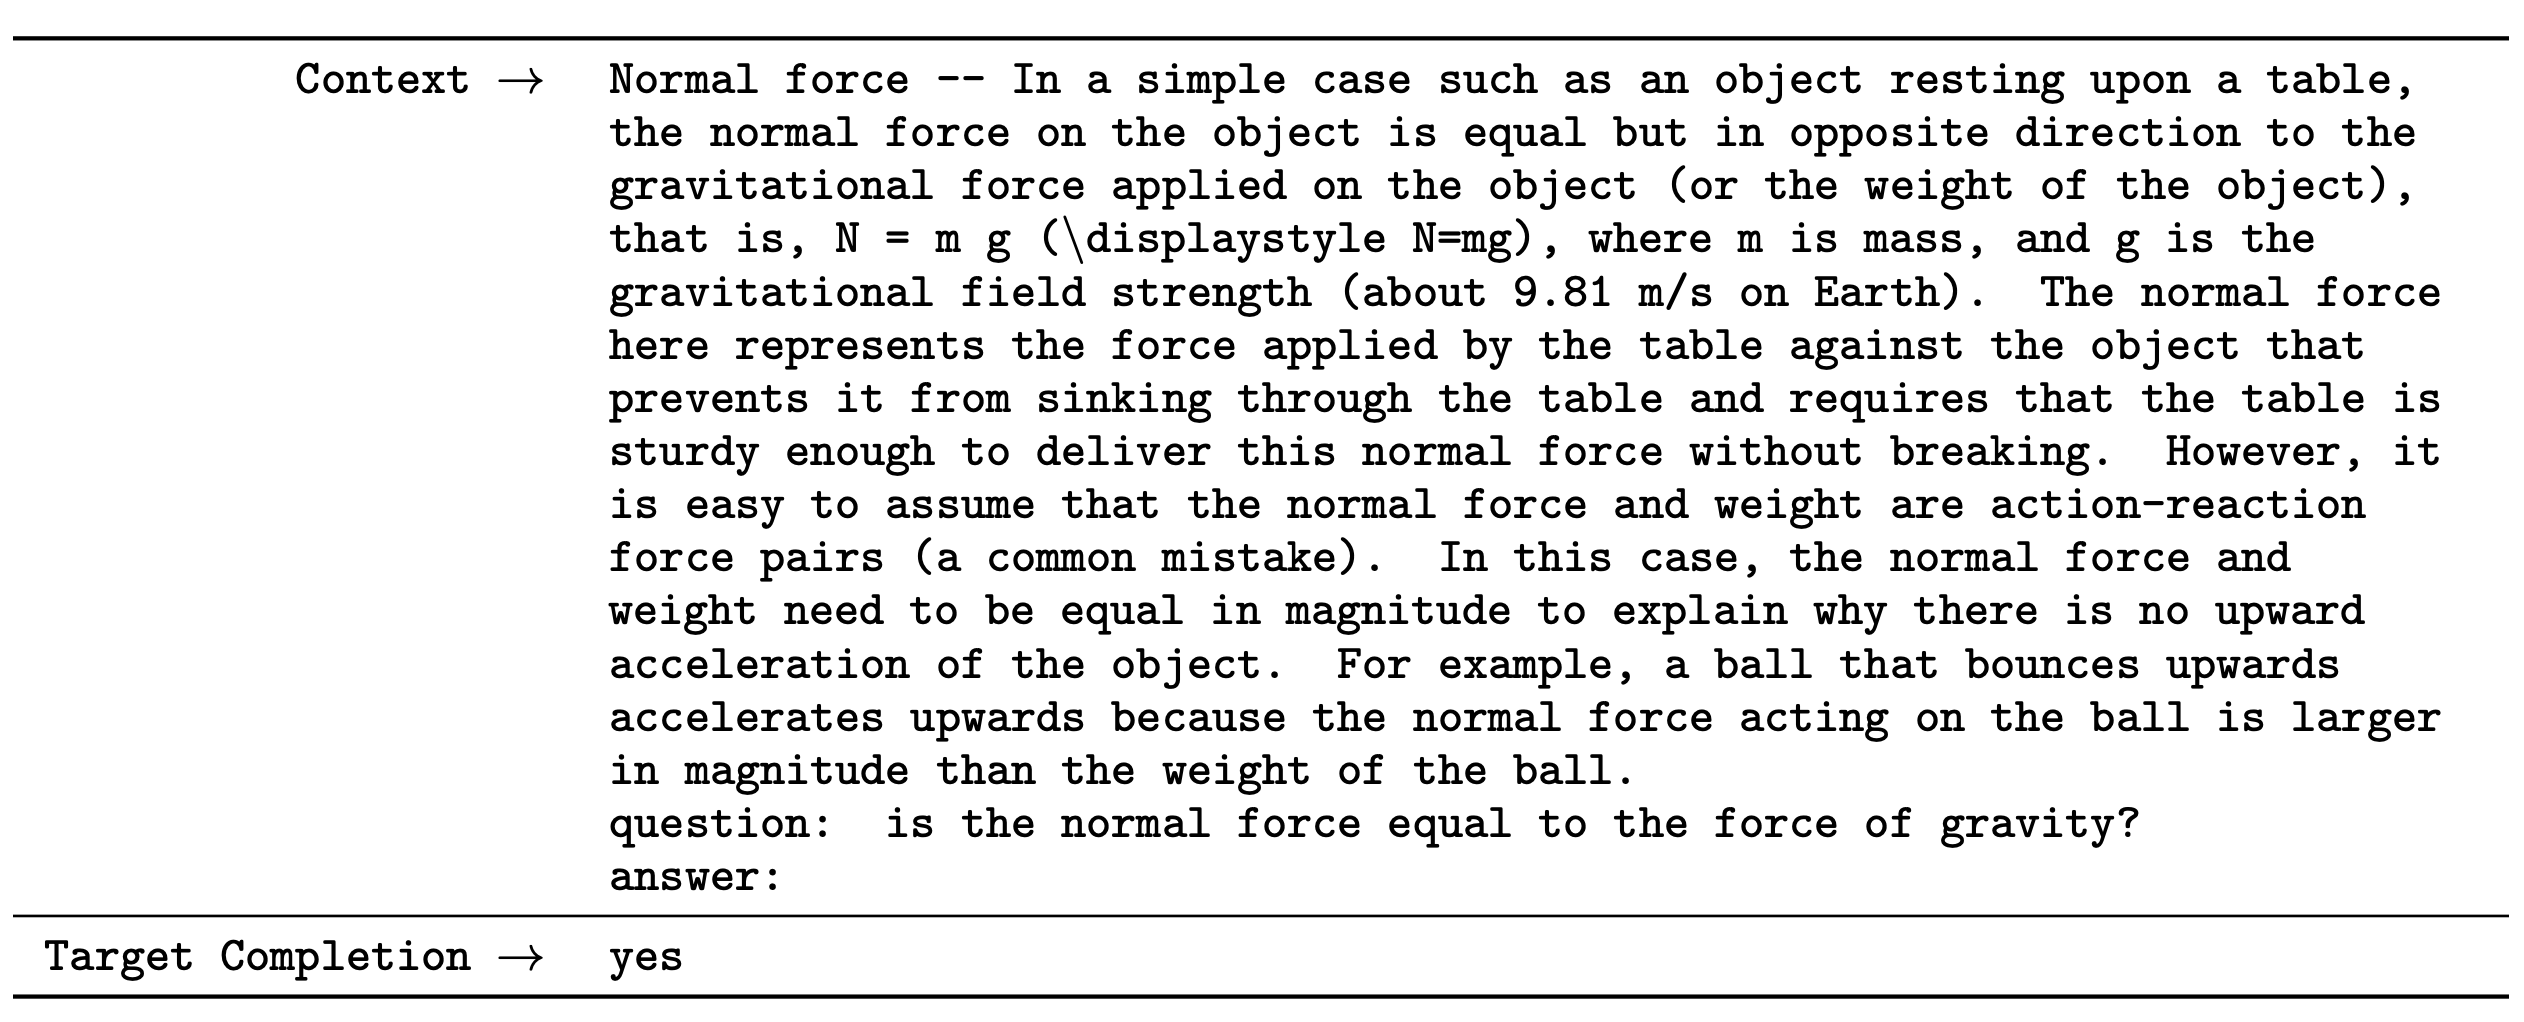
\includegraphics[width=10cm]{figure/boolqtask.png}
	\end{figure}

\vfill

\end{frame}



% ------------------------------------------------------------------------------

\begin{frame}{WiC (Word in Context) task}

\vfill

	\begin{figure}
		\centering
		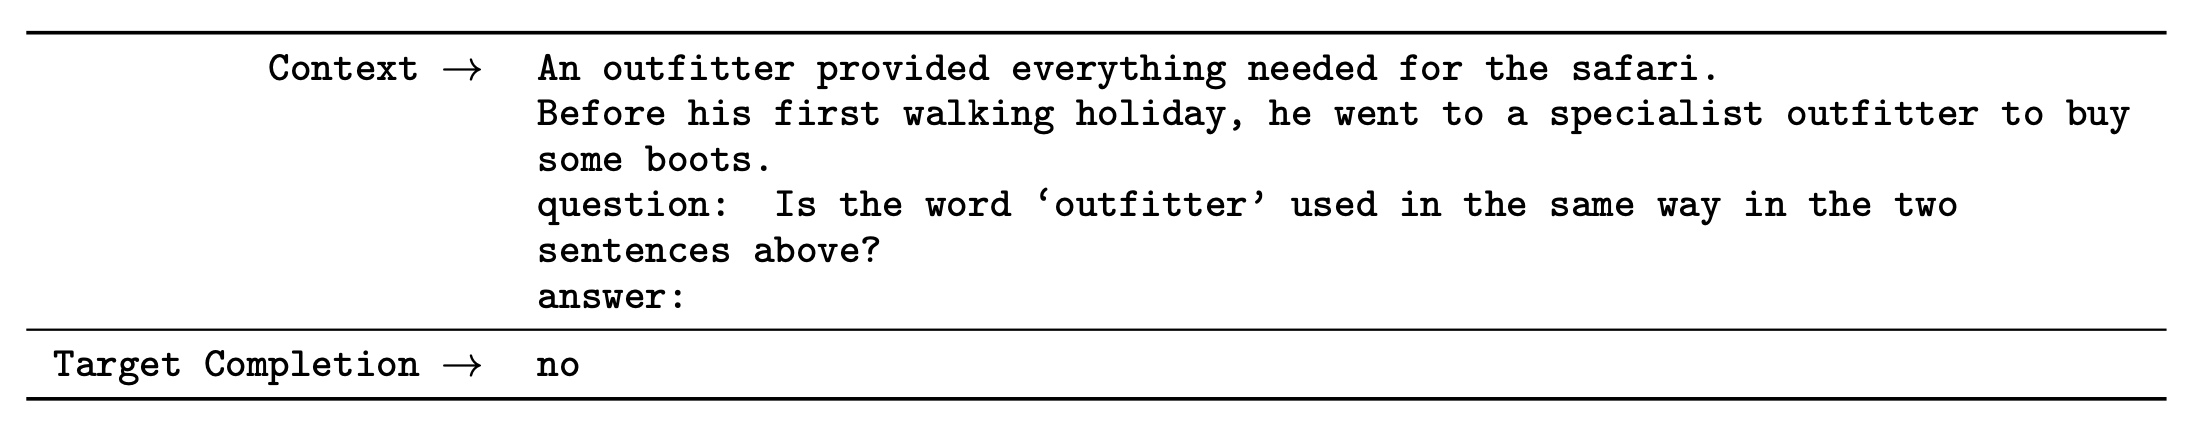
\includegraphics[width=10cm]{figure/wicperf.png}
	\end{figure}

\vfill

\end{frame}



% ------------------------------------------------------------------------------

\begin{frame}{COPA task}

\vfill

	\begin{figure}
		\centering
		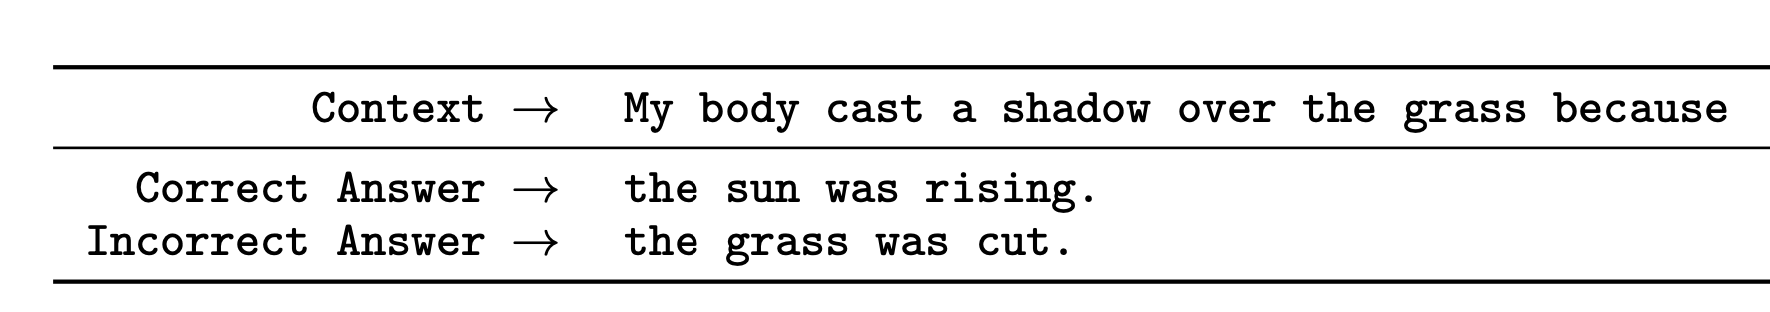
\includegraphics[width=10cm]{figure/copaperf.png}
	\end{figure}

\vfill

\end{frame}



% ------------------------------------------------------------------------------

\begin{frame}{WSC (Winograd Schema Challenge) task}

\vfill

	\begin{figure}
		\centering
		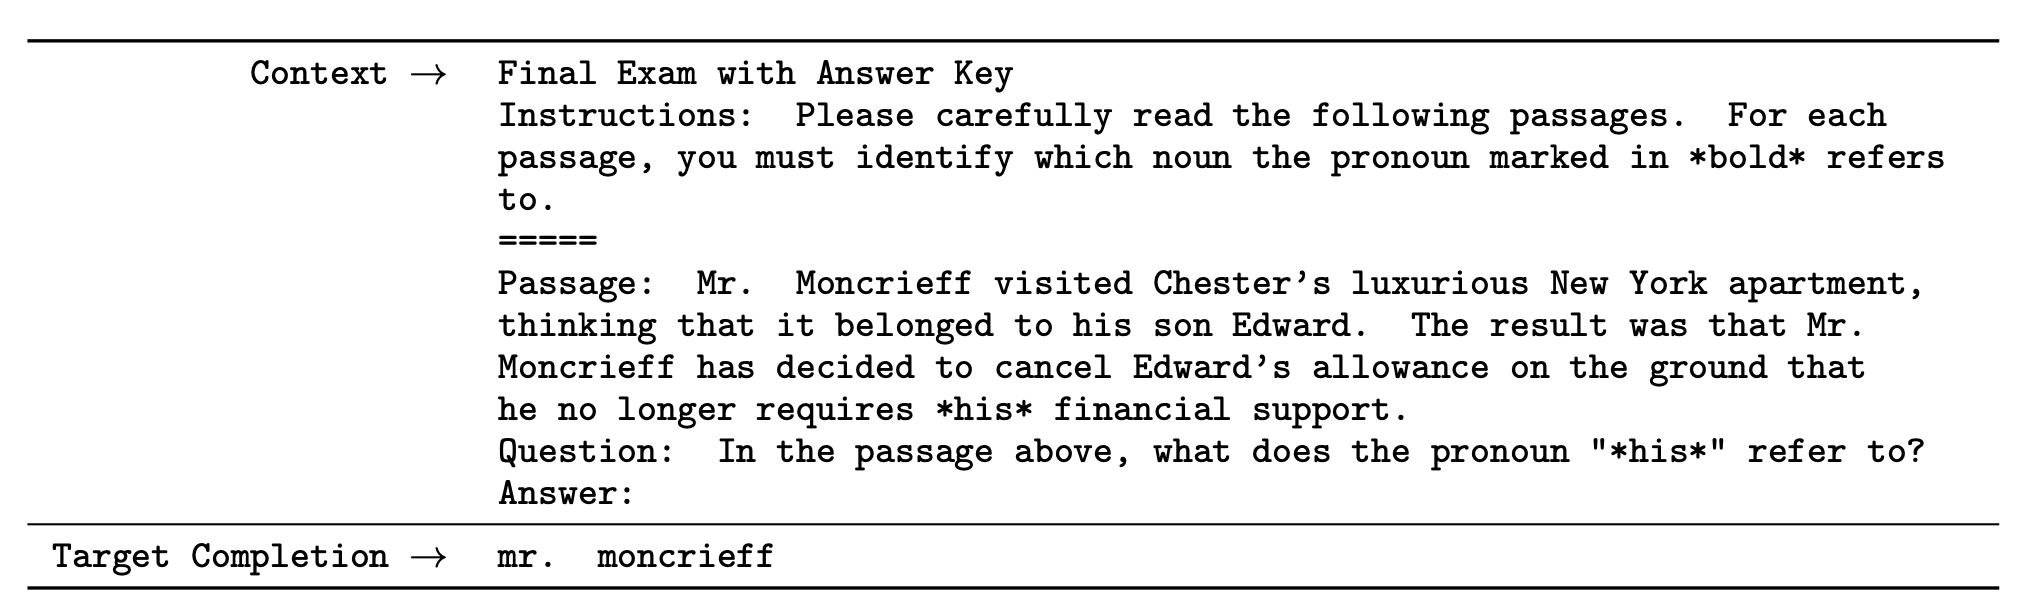
\includegraphics[width=10cm]{figure/wscformat.png}
	\end{figure}

\vfill

\end{frame}



% ------------------------------------------------------------------------------

\begin{frame}{ReCoRD task}

\vfill

	\begin{figure}
		\centering
		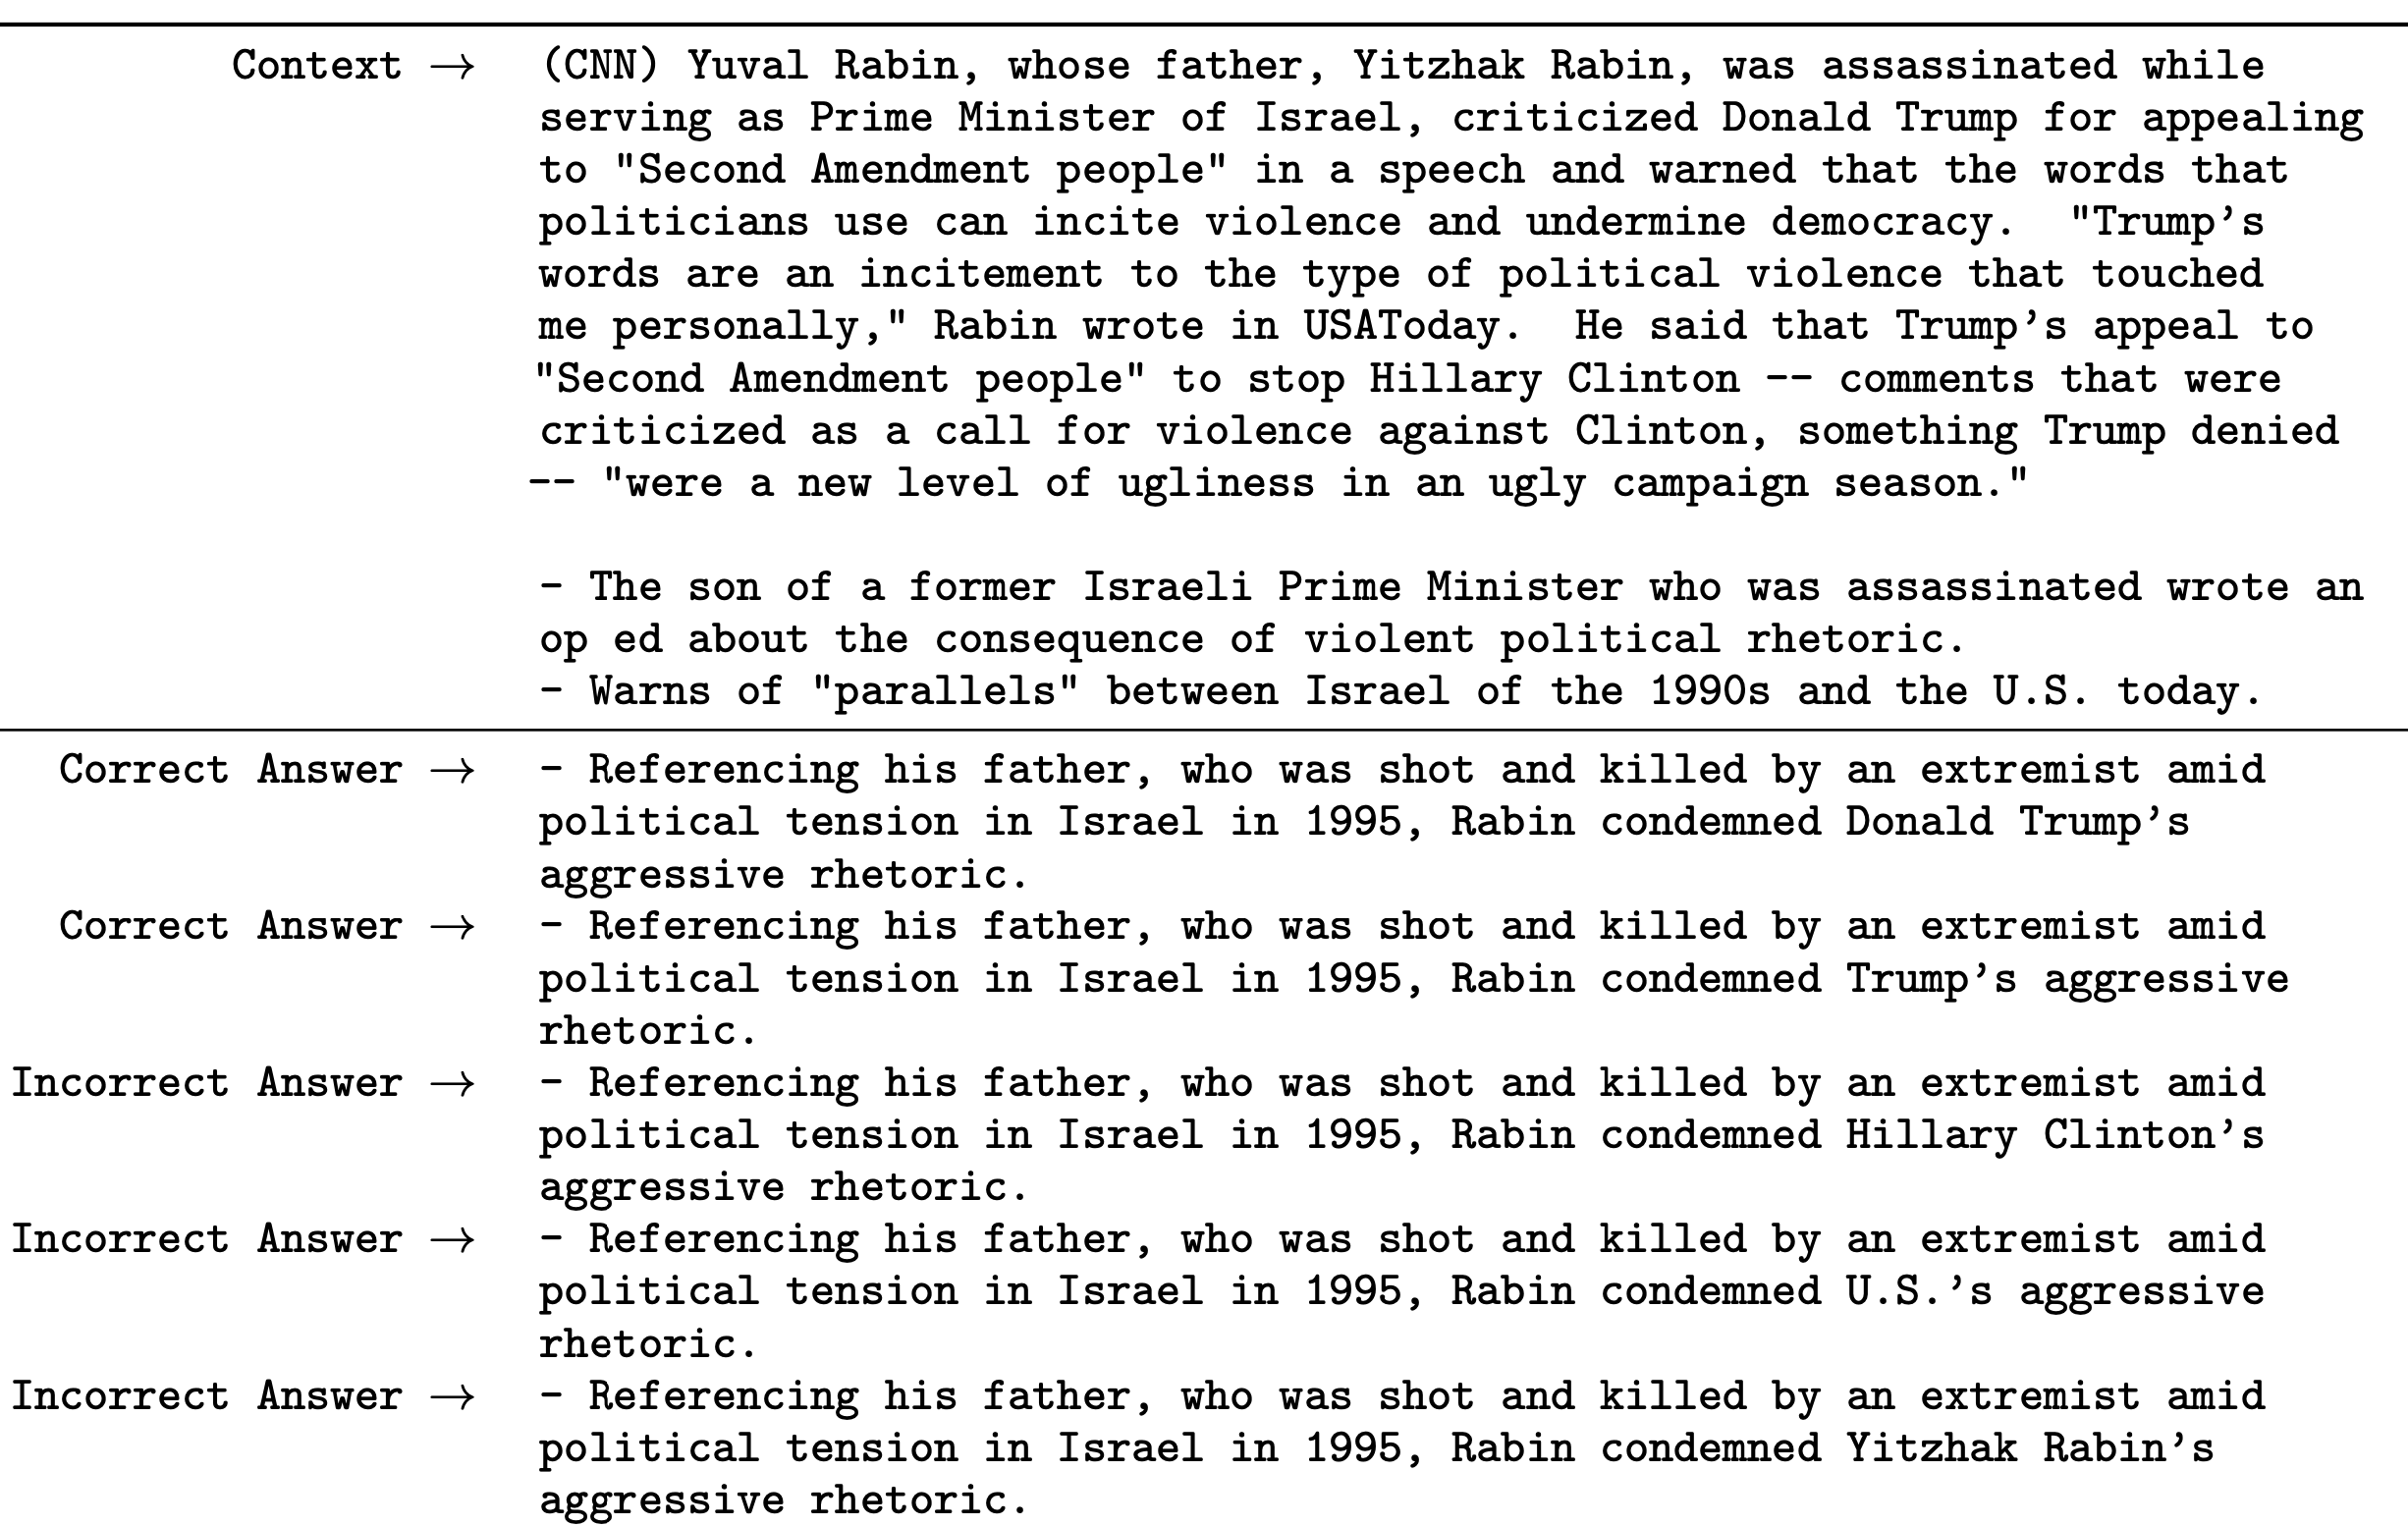
\includegraphics[width=10cm]{figure/recordformat.png}
	\end{figure}

\vfill

\end{frame}



% ------------------------------------------------------------------------------

\begin{frame}{ANLI task}

\vfill

	\begin{figure}
		\centering
		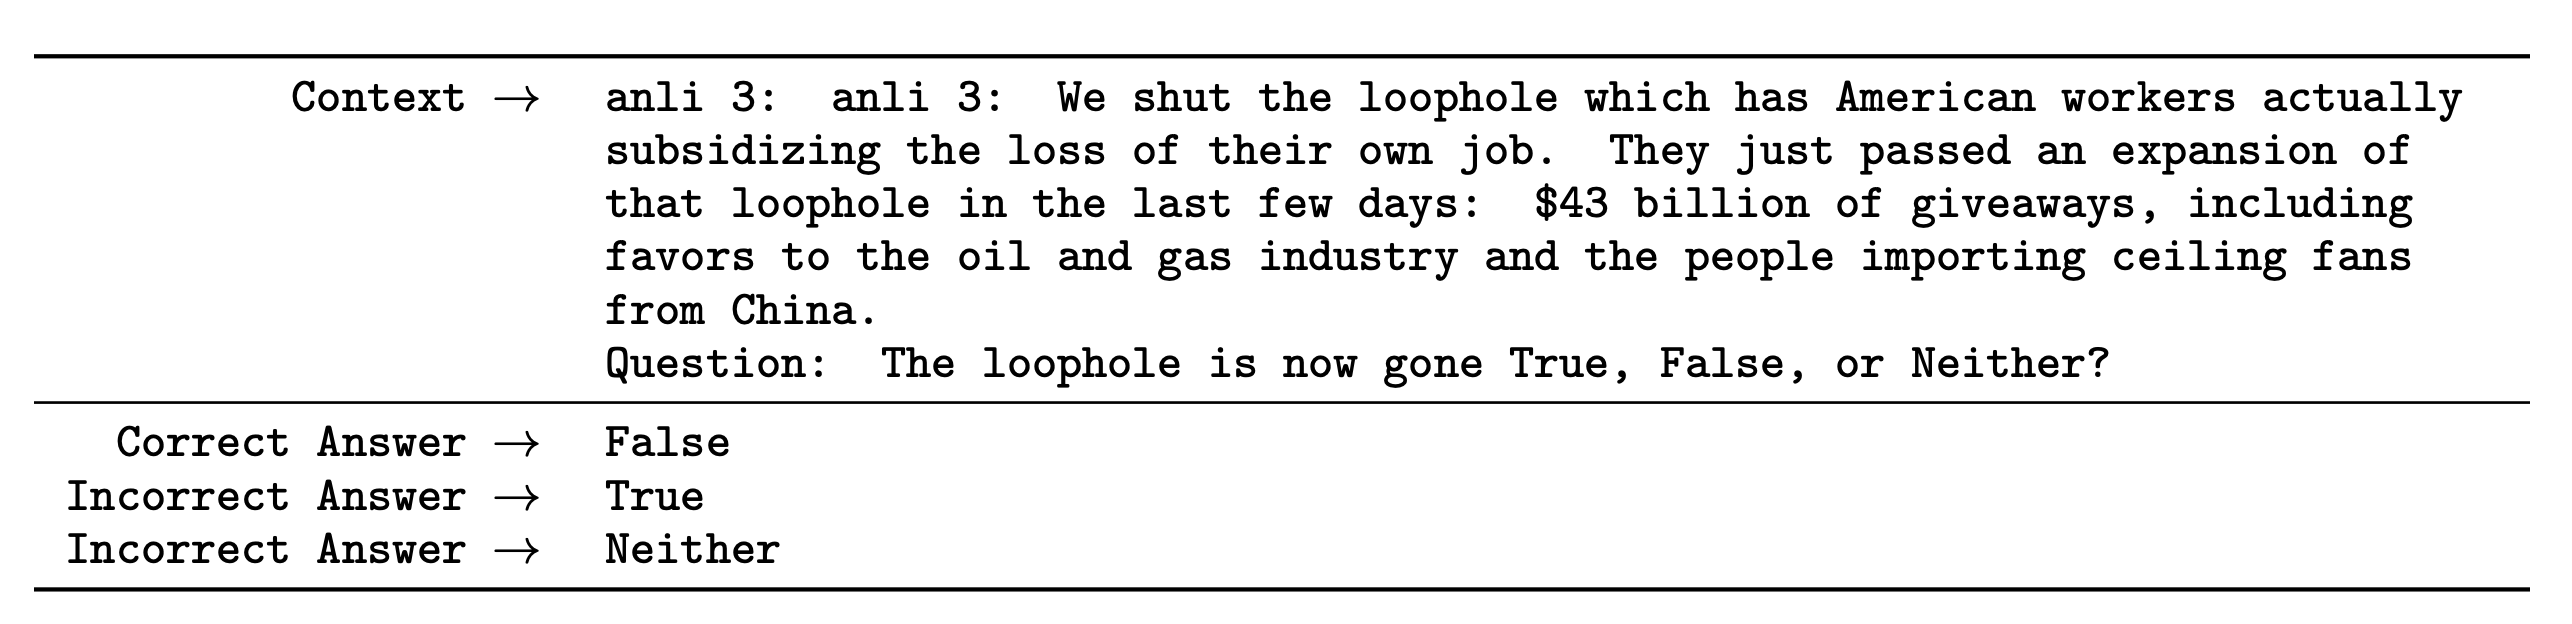
\includegraphics[width=10cm]{figure/anliformat.png}
	\end{figure}

\vfill

\end{frame}



% ------------------------------------------------------------------------------

\begin{frame}{Performance on ANLI task}

\vfill

	\begin{figure}
		\centering
		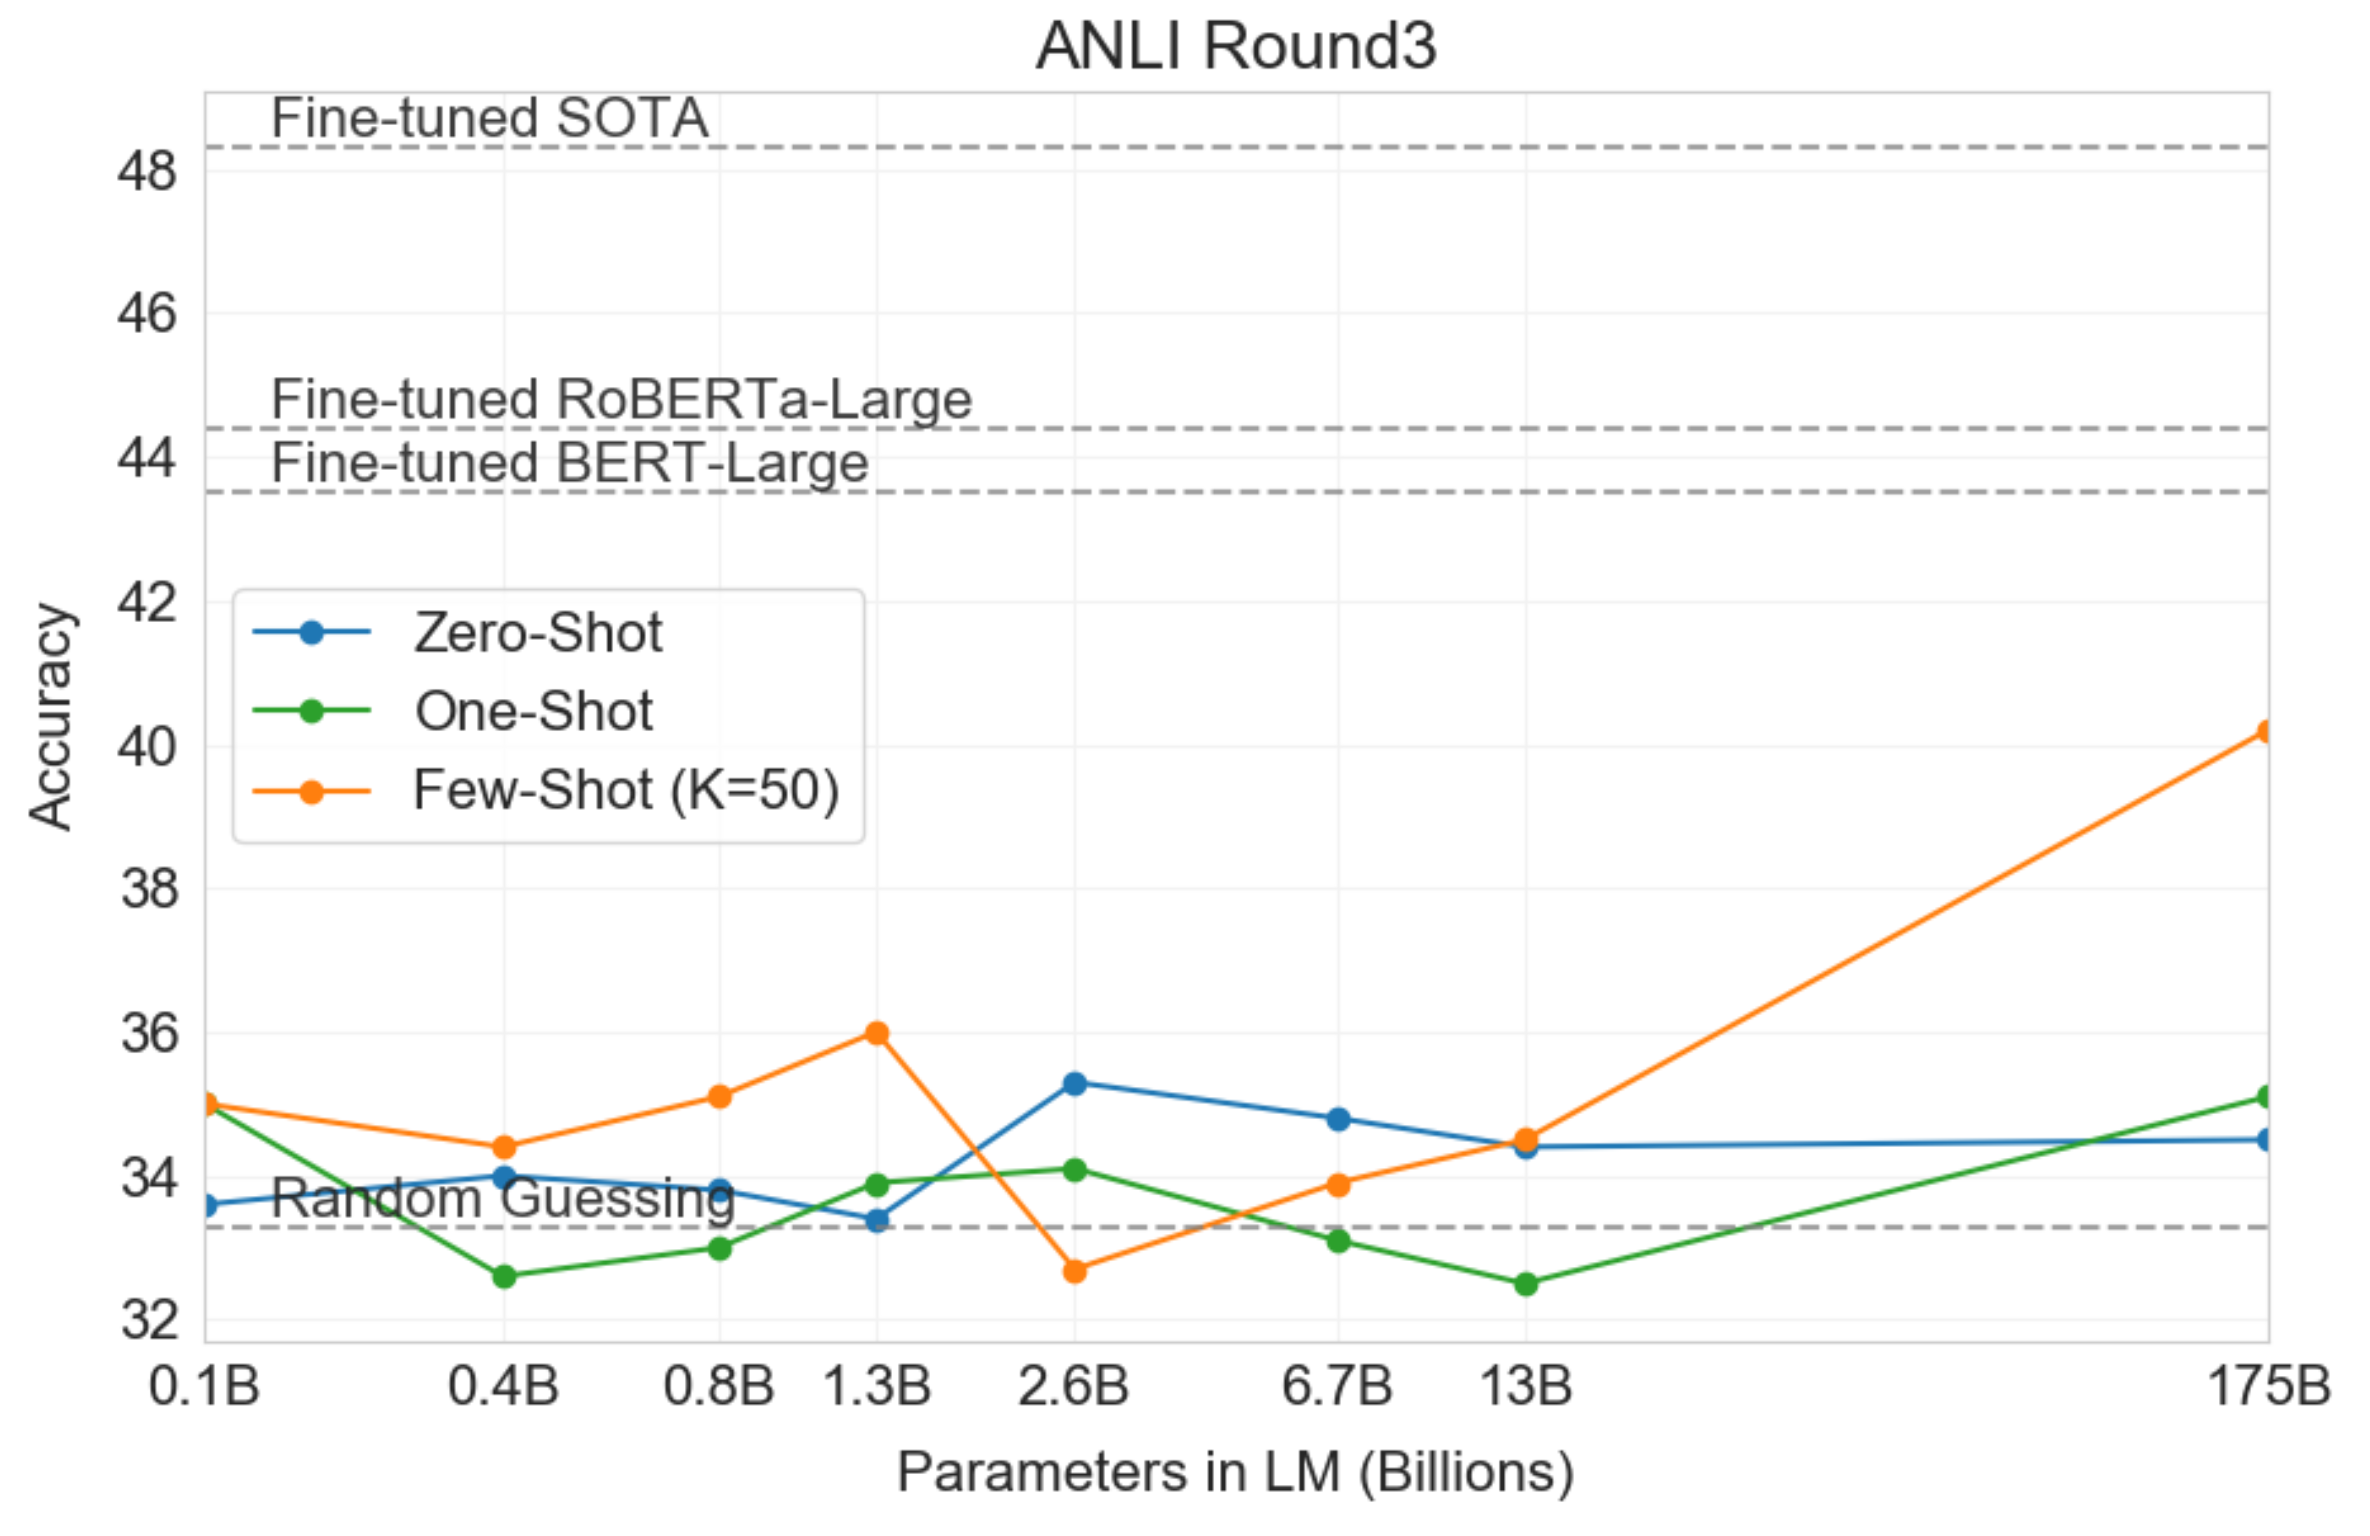
\includegraphics[width=10cm]{figure/anliperf.png}
	\end{figure}

\vfill

\end{frame}



% ------------------------------------------------------------------------------

\begin{frame}{SAT Analogies task}

\vfill

	\begin{figure}
		\centering
		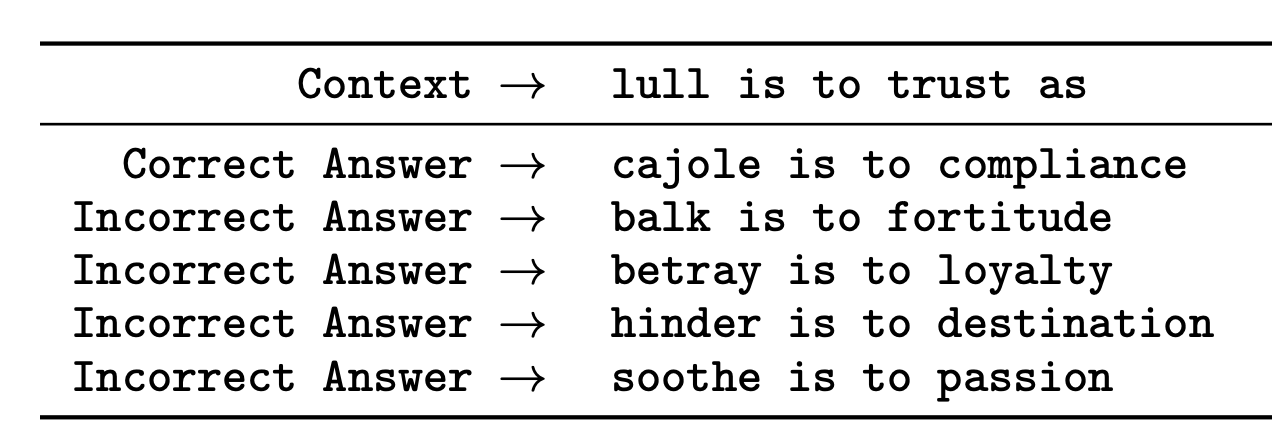
\includegraphics[width=10cm]{figure/satformat.png}
	\end{figure}

\vfill

\end{frame}



% ------------------------------------------------------------------------------

\begin{frame}{Performance on SAT Analogies}

\vfill

	\begin{figure}
		\centering
		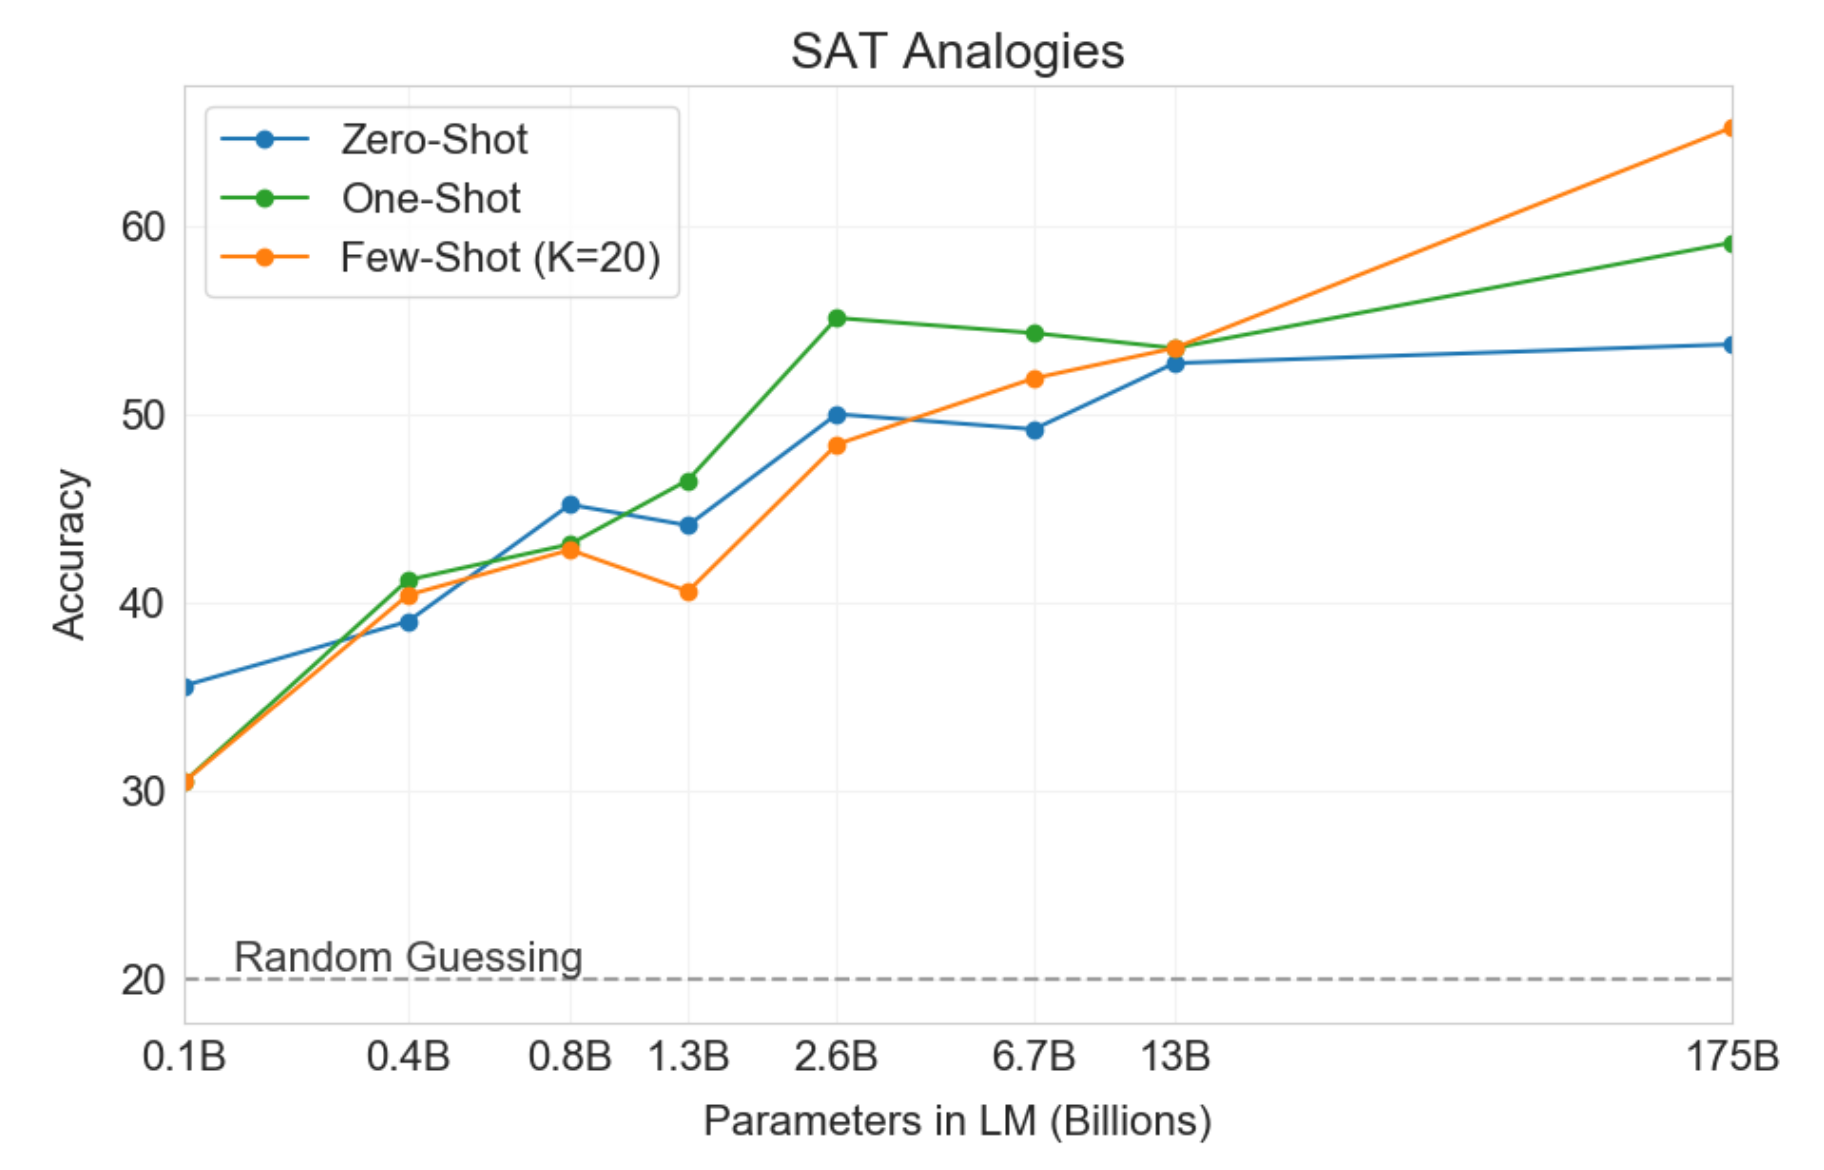
\includegraphics[width=10cm]{figure/satperf.png}
	\end{figure}

\vfill

\end{frame}



% ------------------------------------------------------------------------------

\begin{frame}{GPT3 can correct grammar}

\vfill

	\begin{figure}
		\centering
		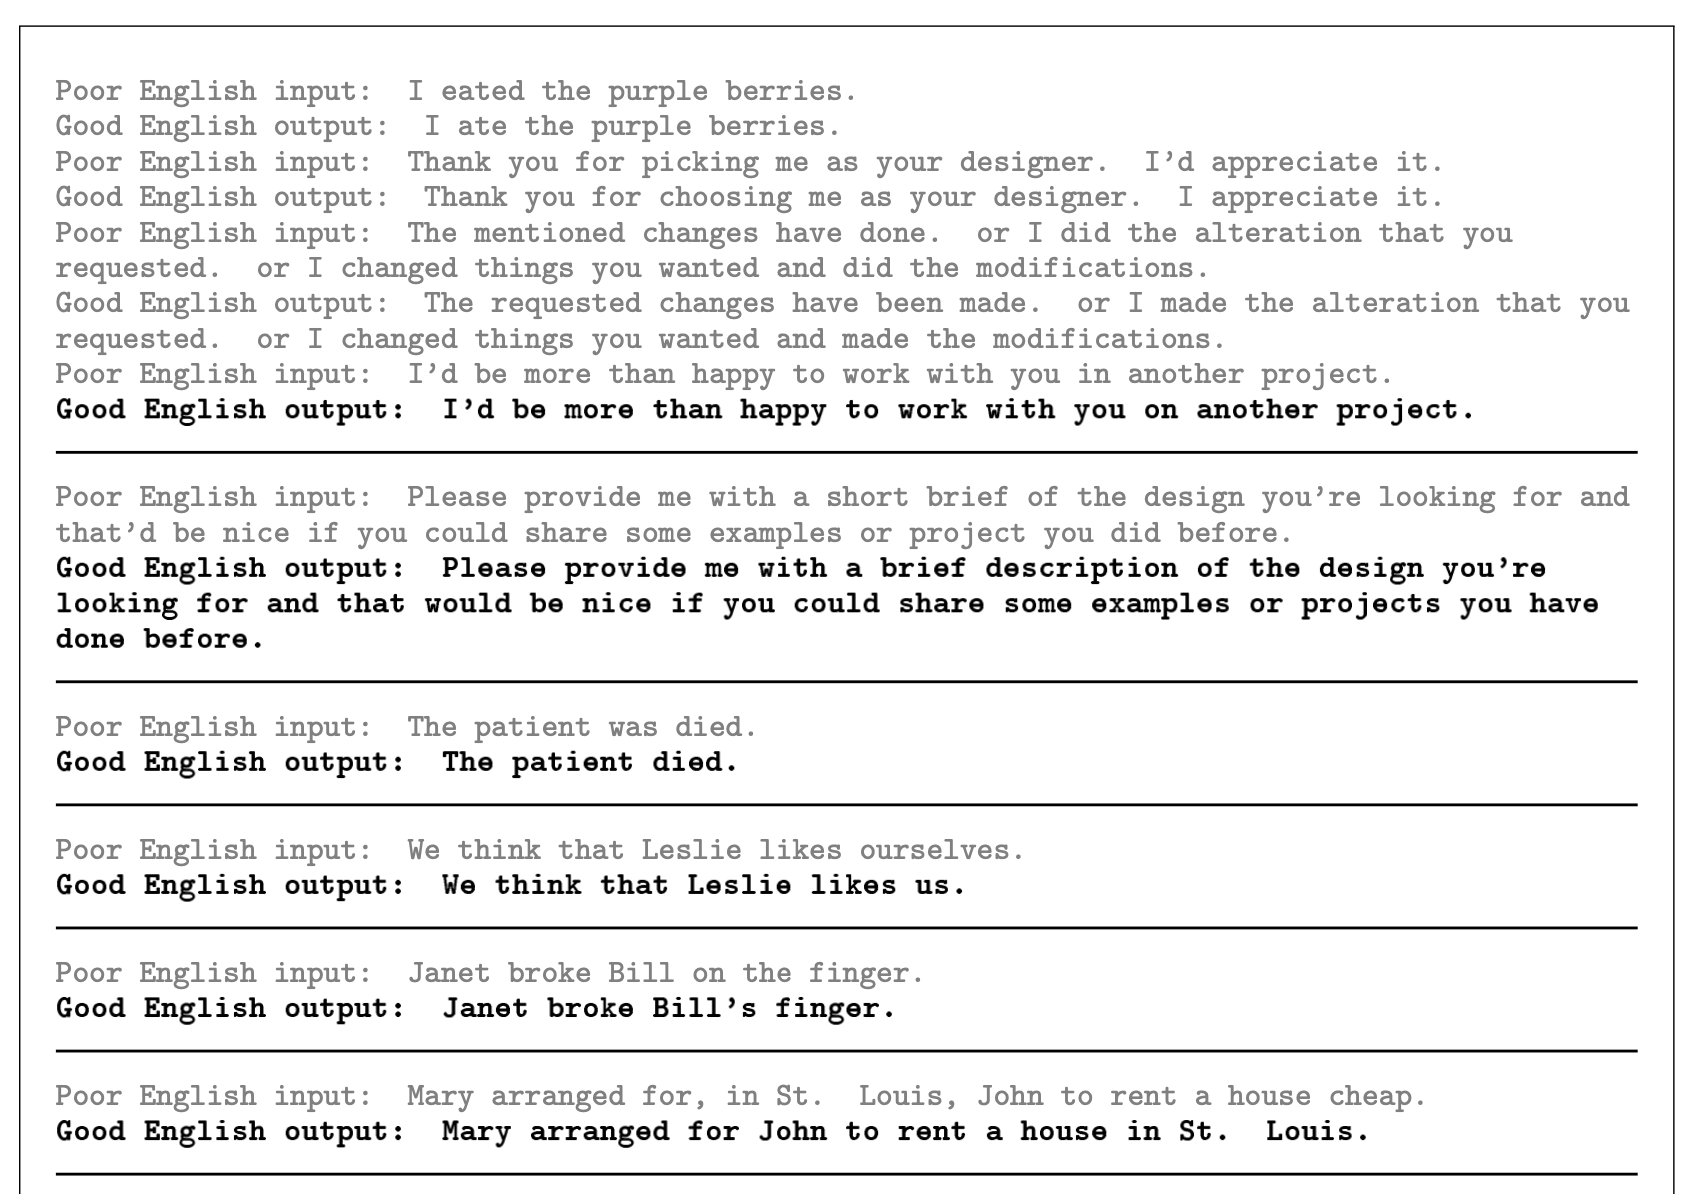
\includegraphics[width=8.50cm]{figure/correctgrammar.png}
	\end{figure}

\vfill

\end{frame}



% ------------------------------------------------------------------------------

\begin{frame}{Generation of news articles}

\vfill

  \begin{itemize}
\pause\item Context given to gpt3:
  \begin{itemize}
\pause\item Three ``training'' articles to condition gpt3
\pause\item Title and subtitle of a 4th article
    \end{itemize}
\pause\item gpt3 then has to generated the body of the 4th article
\pause\item Evaluation: Humans are presented the
human-generated original article and the gpt3-generated
article and are asked to identify which is fake.
    \end{itemize}

\vfill

\end{frame}



% ------------------------------------------------------------------------------

\begin{frame}{Humans cannot distinguish human generated vs GPT-3 generated}

\vfill

	\begin{figure}
		\centering
		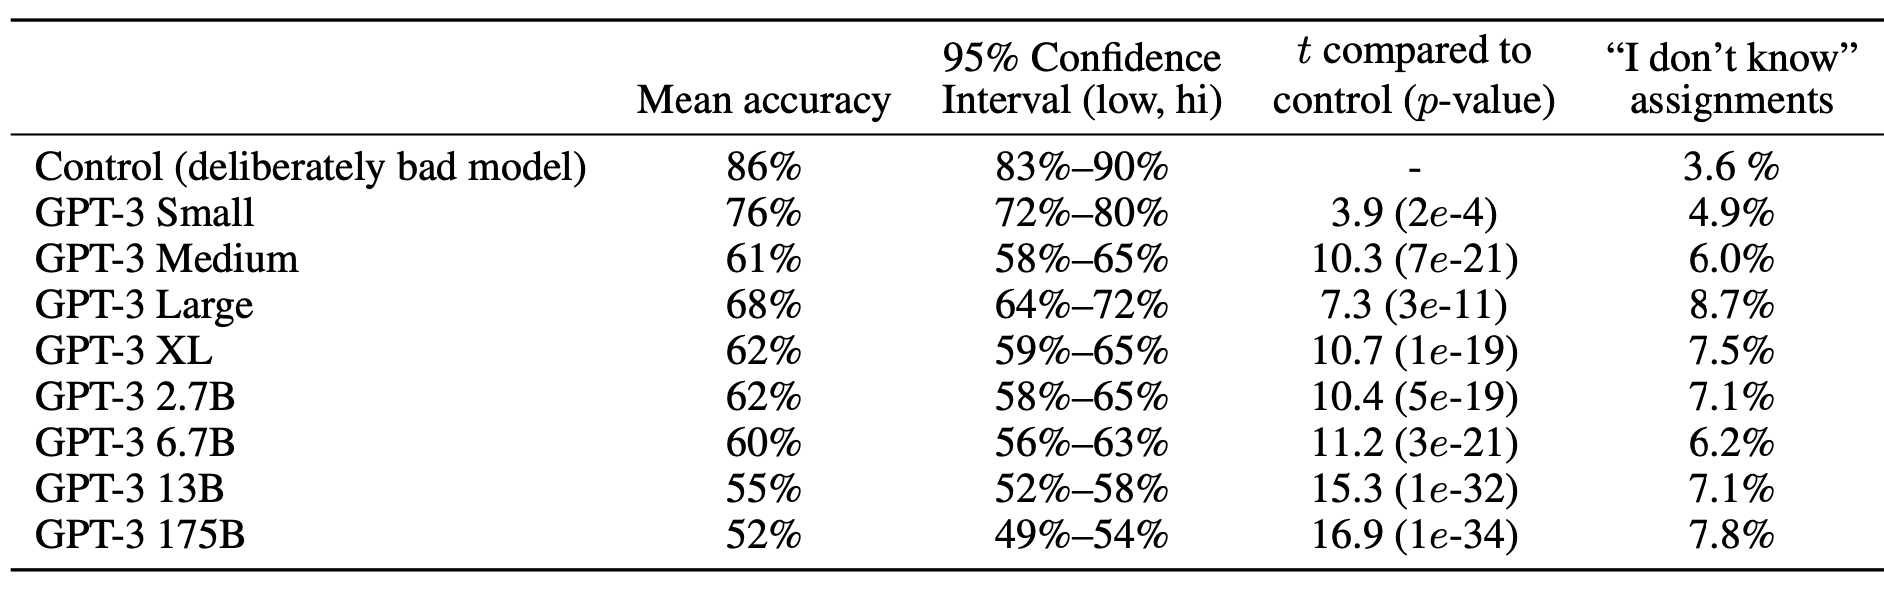
\includegraphics[width=10cm]{figure/humanvsmachine.png}
	\end{figure}

\vfill

\end{frame}



% ------------------------------------------------------------------------------

\begin{frame}{Hard to identify as fake}

\vfill

	\begin{figure}
		\centering
		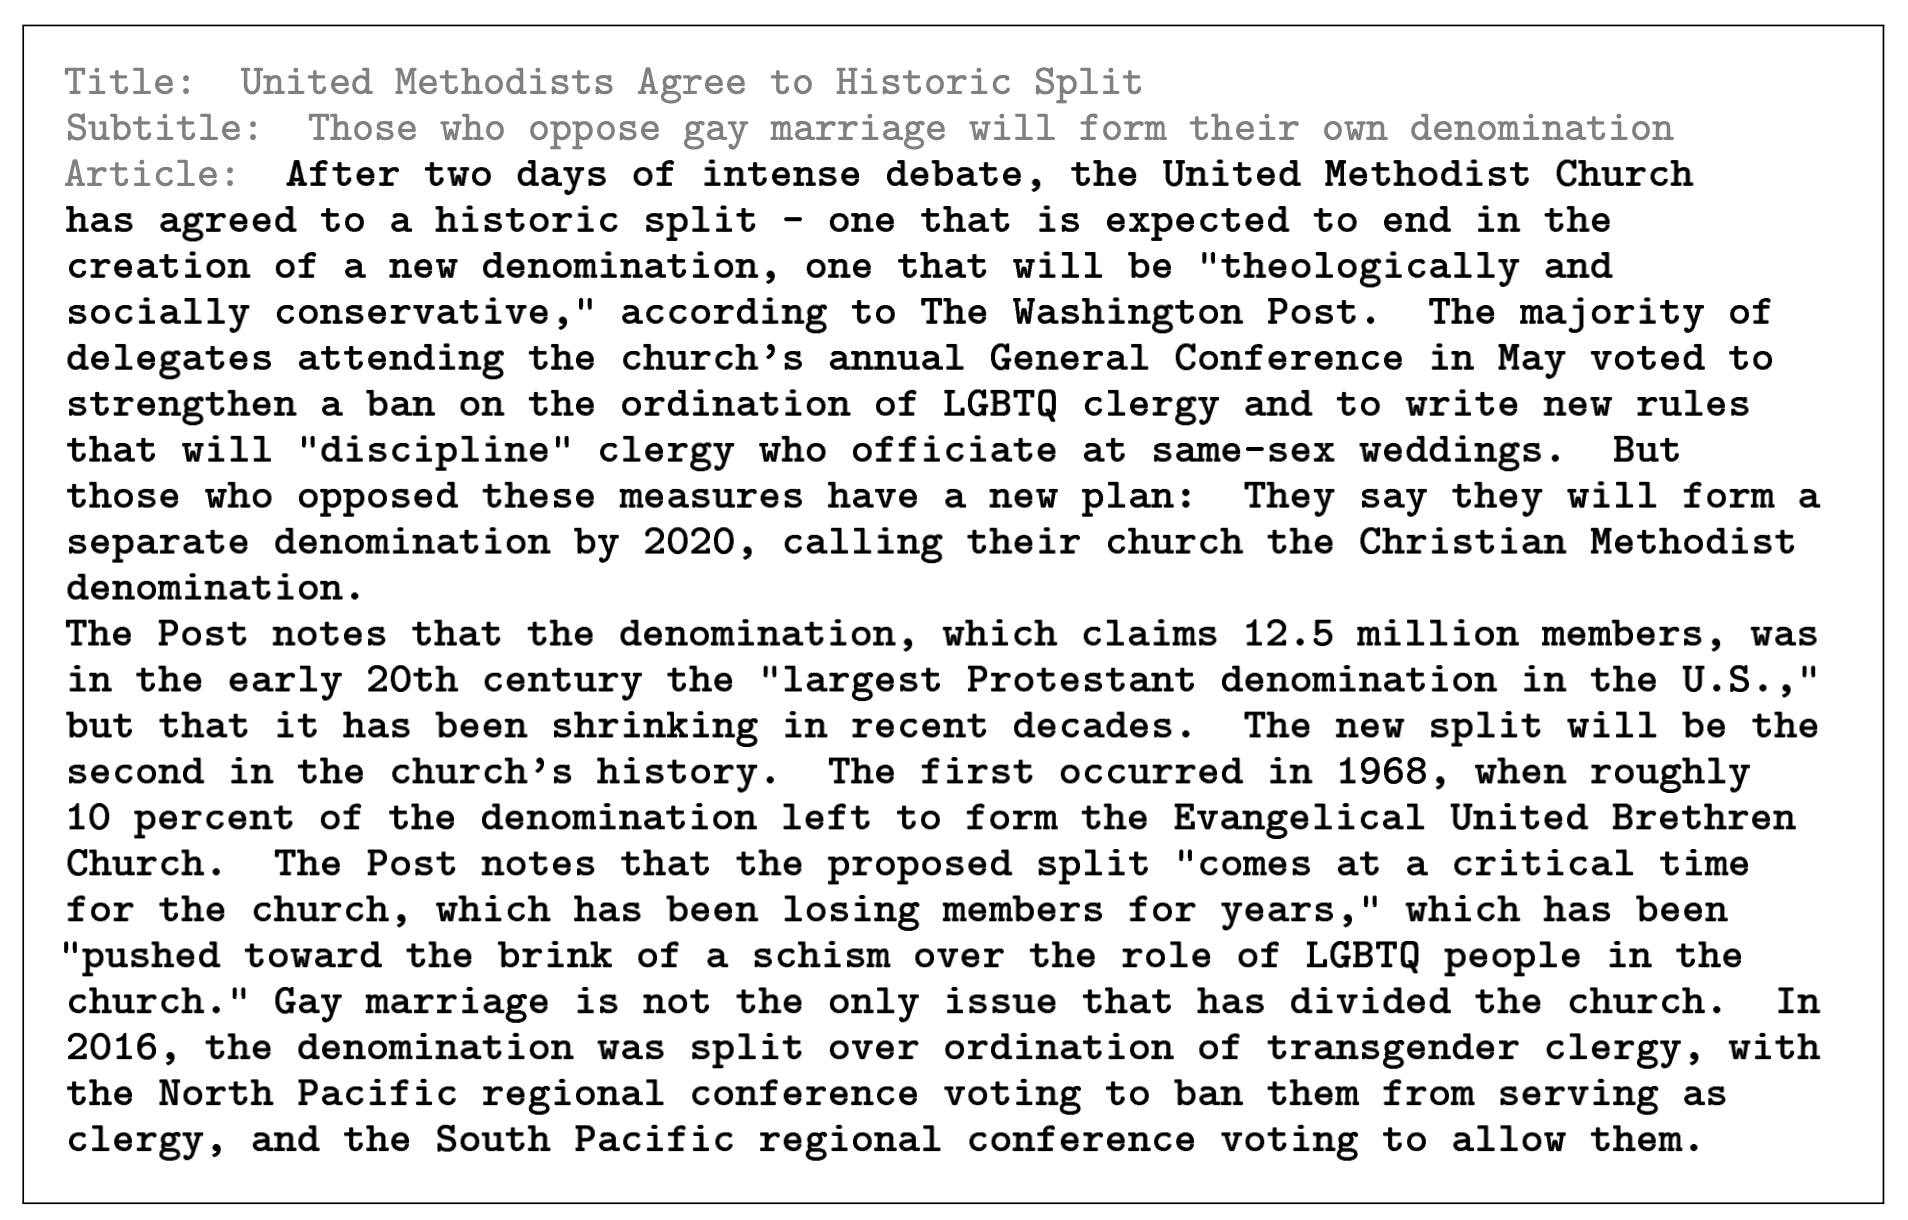
\includegraphics[width=10cm]{figure/hardtoidentify.png}
	\end{figure}

\vfill

\end{frame}



% ------------------------------------------------------------------------------

\begin{frame}{Easier to identify as fake}

\vfill

	\begin{figure}
		\centering
		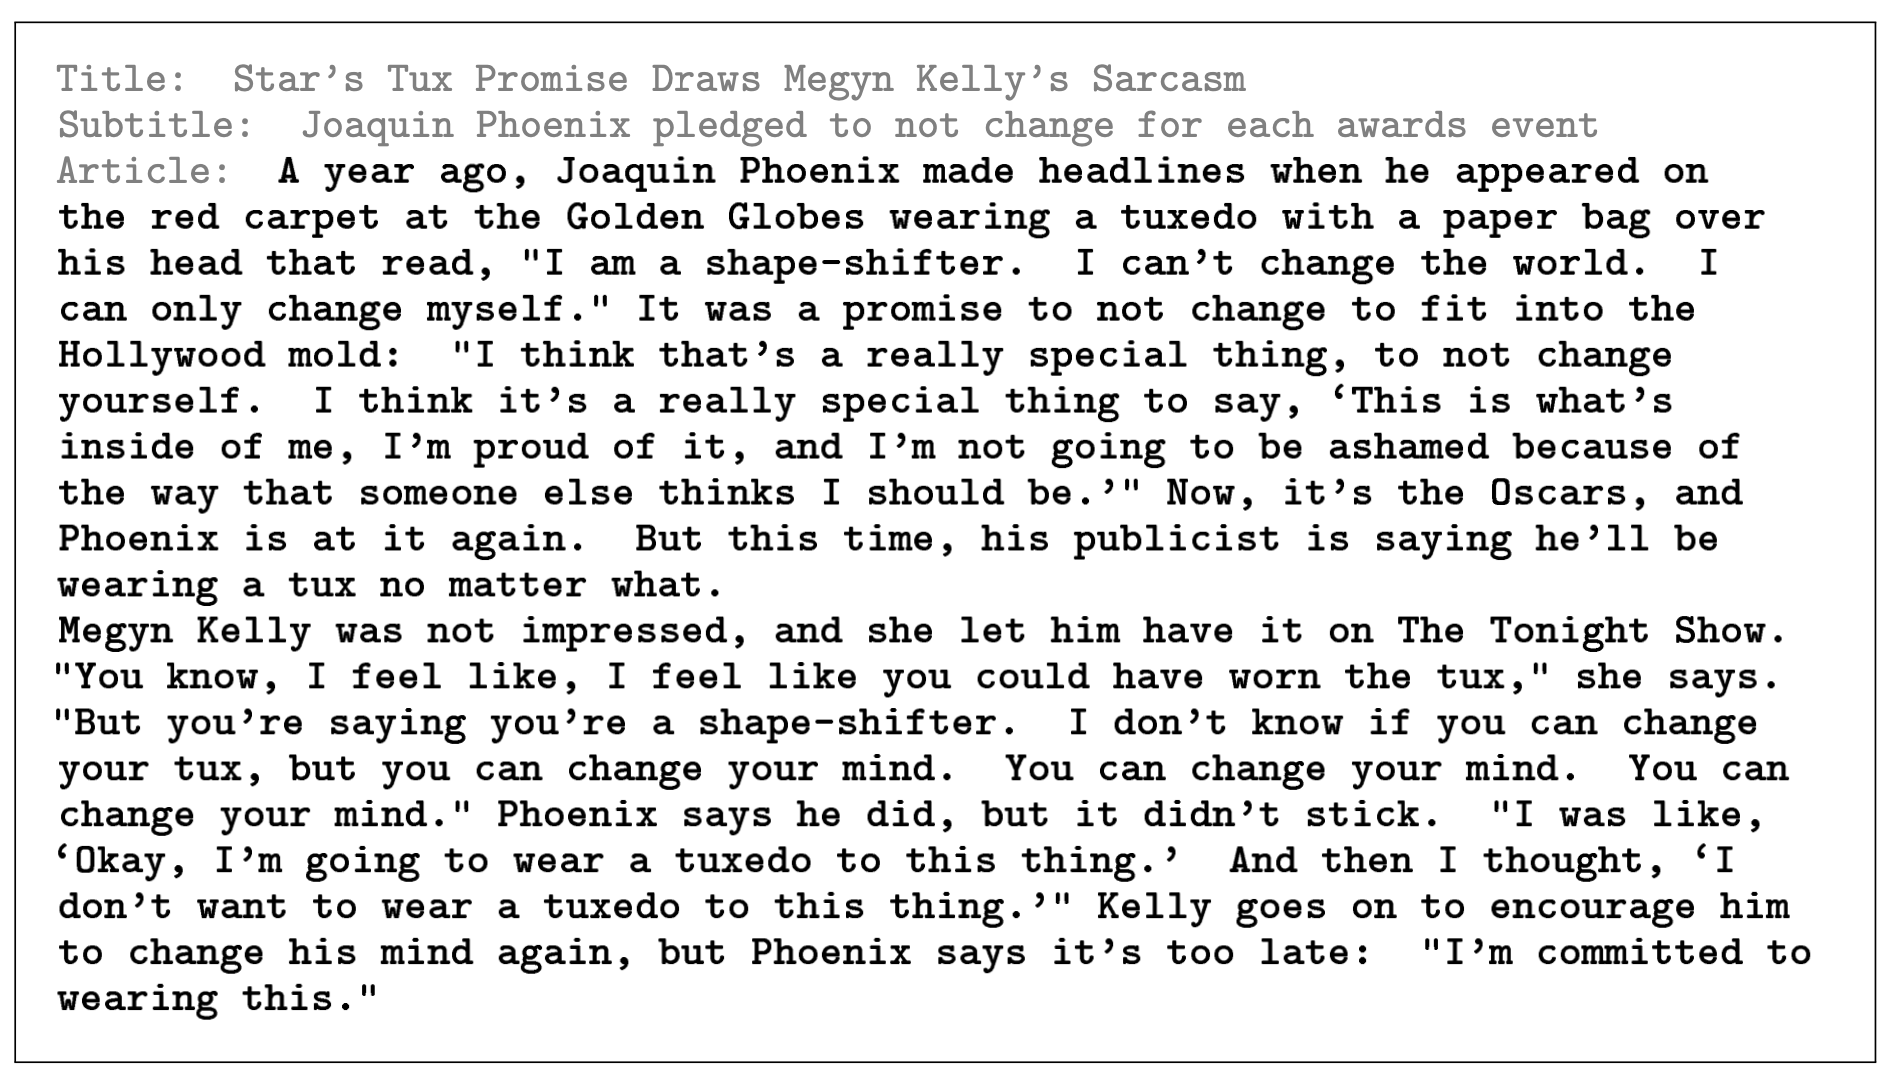
\includegraphics[width=10cm]{figure/easytoidentify.png}
	\end{figure}

\vfill

\end{frame}



% ------------------------------------------------------------------------------

\begin{frame}{Summary}

\vfill

  \begin{itemize}
\item The average person has difficulty distinguishing
human-generated and gpt3-generated news.
\item However, the non-average person probably can
distinguish them quite well.
\item It is unclear whether  machines
are able to distinguish
human-generated from gpt3-generated news.
\item This has great significance for preventing abuse
of AI technology.
  \end{itemize}

\vfill

\end{frame}


%%%%%%%%%%%%%%%%%%%%%%%%%%%%%%%%%%%%%%%%%%%%%%%%%%%%%%%%%%%%%%%%%%
\section{GPT-3: Ethics \& Cost}
% Source: DL4NLP chapter07-gpt/slides-75-discussion.tex
%%%%%%%%%%%%%%%%%%%%%%%%%%%%%%%%%%%%%%%%%%%%%%%%%%%%%%%%%%%%%%%%%%
% ------------------------------------------------------------------------------

\begin{frame}{History of GPT}

\vfill

\begin{itemize}
\item Three OpenAI papers
\item GPT (2018): Improving language understanding by
generative pre-training
\item GPT2 (2019): Language Models are Unsupervised Multitask Learners
\item GPT3 (2020): Language Models are Few-Shot Learners 
\item We're not interested here in the (small) differences
between these papers and will focus on GPT3, but refer to it
as GPT.
\item Recommendation: Read GPT3 paper

    \end{itemize}

\vfill

\end{frame}

% ------------------------------------------------------------------------------

\begin{frame}{GPT hype (1)}

\vfill

	\begin{figure}
		\centering
		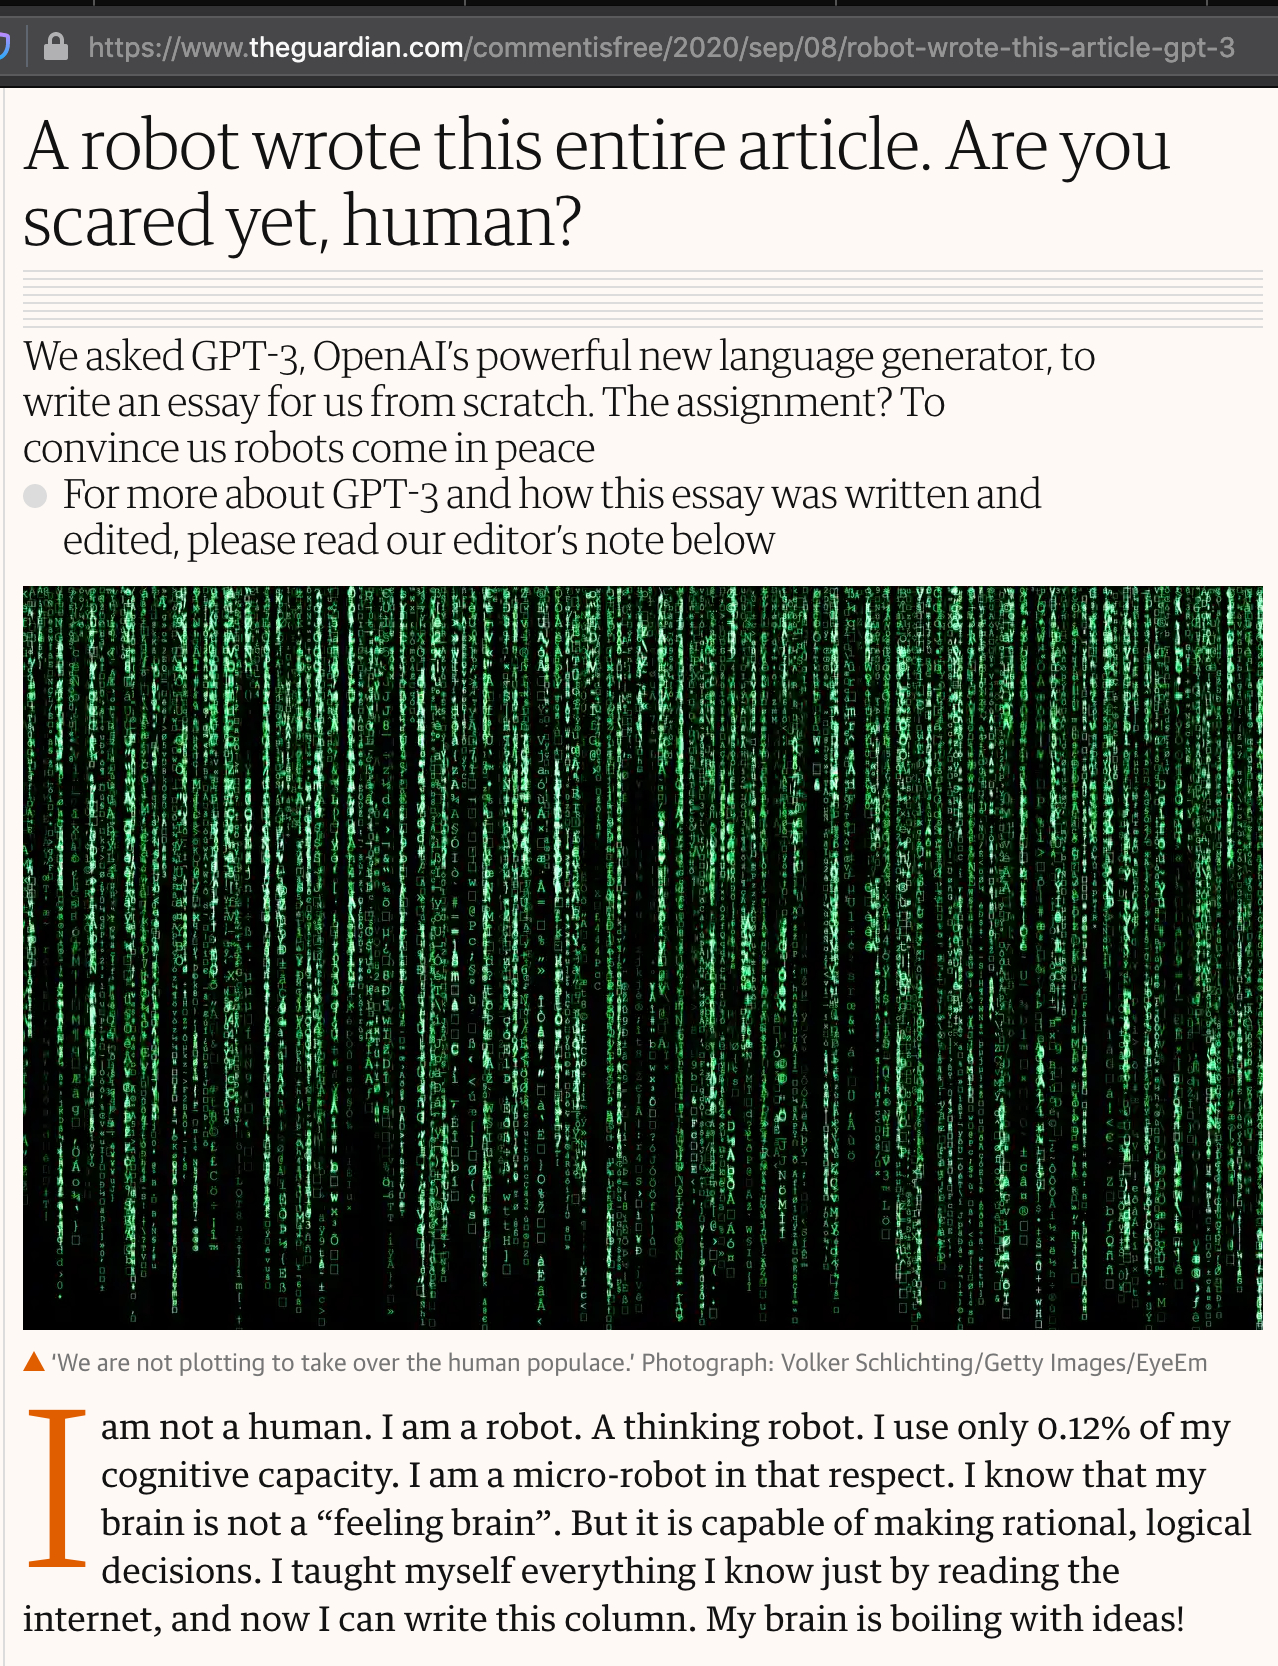
\includegraphics[height=5.95cm,width=6.80cm]{figure/guardian.png}
	\end{figure}

\vfill

\end{frame}

% ------------------------------------------------------------------------------

\begin{frame}{GPT hype (2)}

\vfill

	\begin{figure}
		\centering
		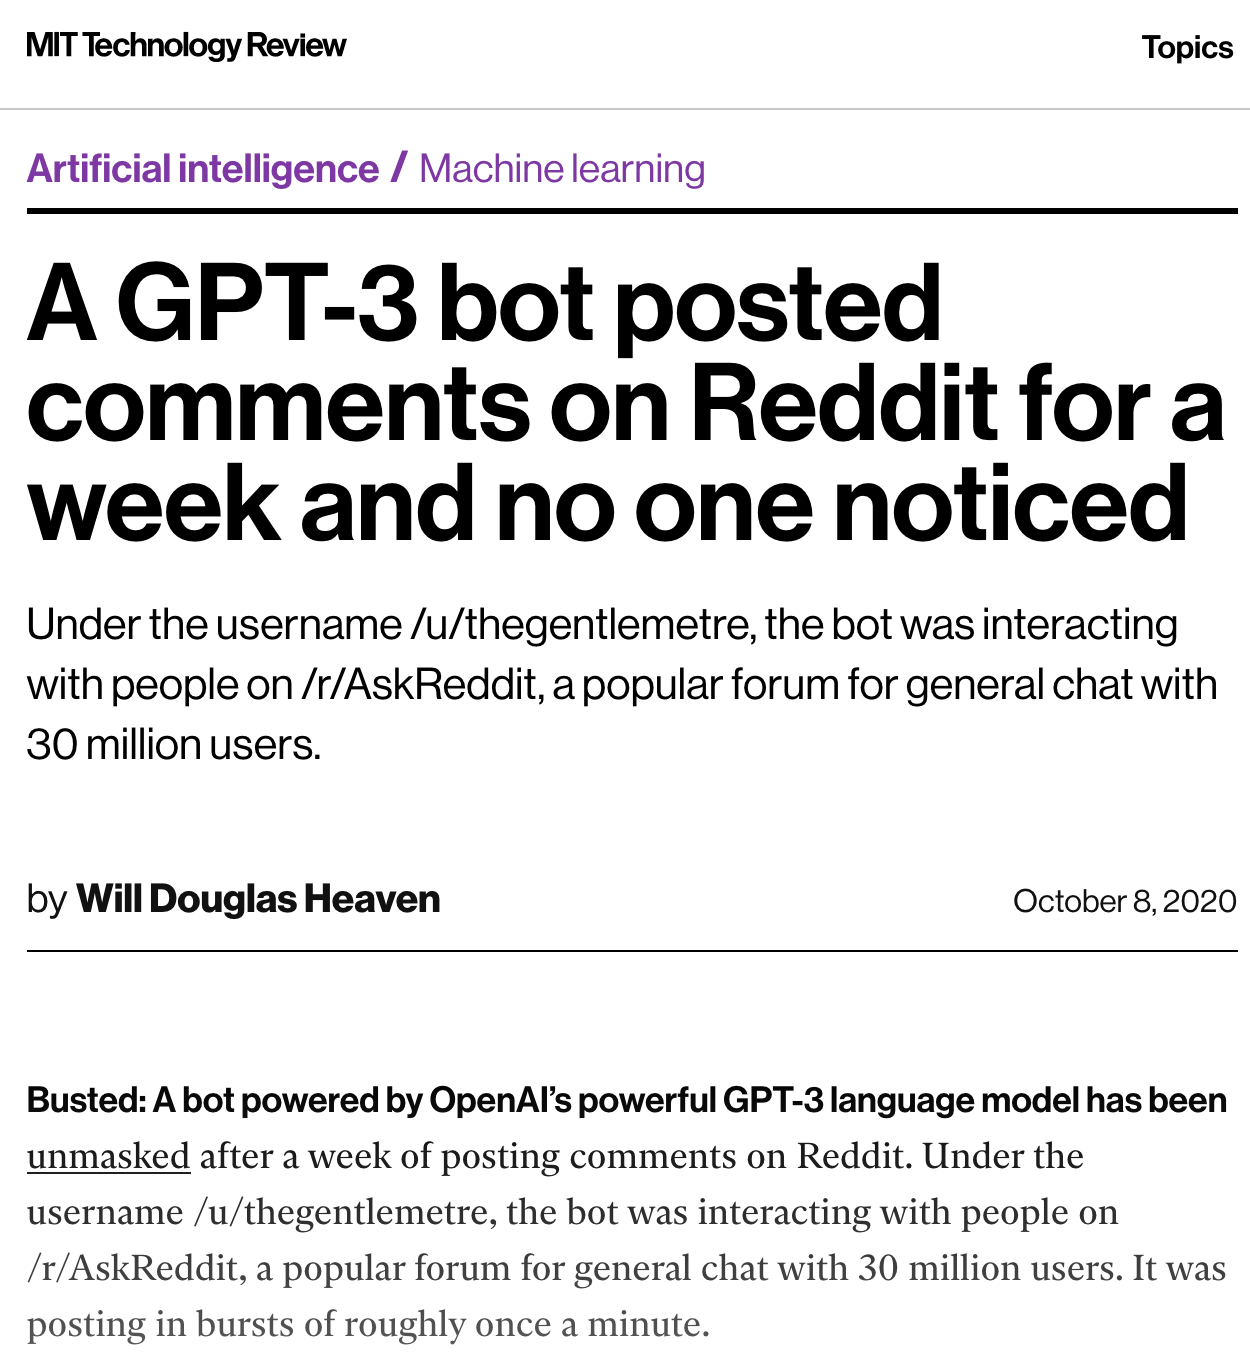
\includegraphics[height=5.95cm,width=6.80cm]{figure/mittechnologyreview.png}
	\end{figure}
	
\vfill

\end{frame}

% ------------------------------------------------------------------------------

\begin{frame}{Cost of training GPT3: \$4.6M?}

\vfill

	\begin{figure}
		\centering
		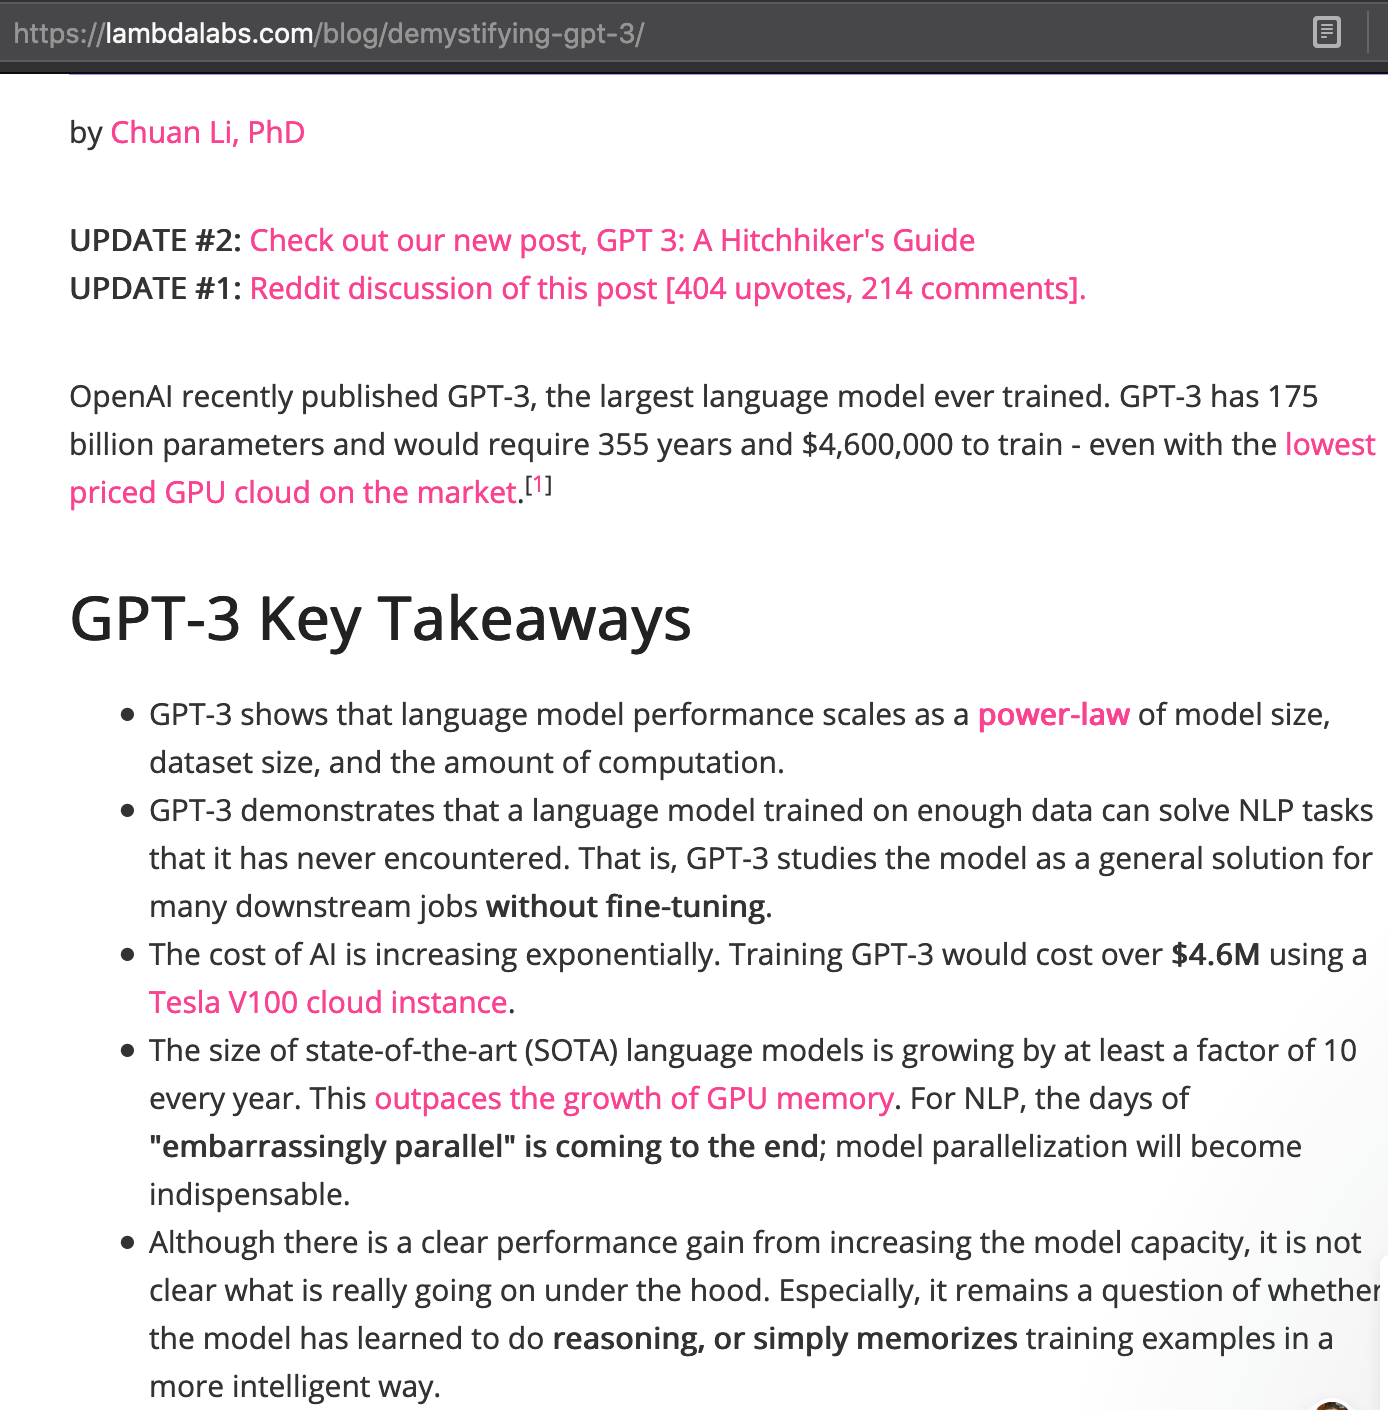
\includegraphics[width=5.95cm]{figure/gpt3cost.png}
	\end{figure}

\vfill

\end{frame}


% ------------------------------------------------------------------------------

\begin{frame}{GPT3 is not environmentally friendly}

\vfill

  \begin{block}{https://lambdalabs.com/blog/demystifying-gpt-3/}
      But to put things into perspective, GPT-3 175B model
      required 3.14E23 FLOPS of computing for training. Even
      at theoretical 28 TFLOPS for V100 and lowest 3 year
      reserved cloud pricing we could find, this will take
      355 GPU-years and cost \$4.6M for a single training
      run.
  \end{block}

\vfill

\end{frame}

\begin{frame}{Stats end of 2023}

\vfill

\begin{itemize}
\item  Cost of training ChatGPT: 1300 mega watt hours
\item Does ChatGPT use 564 mega watt hours per day? (is that
      as much as 19,000 US household use in a day?)
      Estimate: Alex de Vries
\item (notice ratio training vs use)
%(564*365)/10.774 = 19107.10970855763875997772
%https://www.eia.gov/tools/faqs/faq.php?id=97&t=3
\item ChatGPT: 6.8 watt hours per user query (versus 0.3
      watt hours for Google)
\item For every $x$ amount of energy used for running your
      GPUs, you may need an additional $.6x$ to $.85x$ for
      cooling.
\item Source: Prof.\ Dieter Kranzlm\"{u}ller, end of
      November 2023
      \item What about carbon-neutral offerings like Google Cloud?
\end{itemize}

\vfill

\end{frame}


% ------------------------------------------------------------------------------

\begin{frame}{Response to green concerns about GPT3}

\vfill

  \begin{itemize}
\item You only have to train the model once. If you
then use it a lot, that can be efficient.
\item Generating 100 pages of text with GPT3 costs a
few cents in energy -- perhaps ok?
\item Distill the model once it is trained (e.g., Distilbert)
    \end{itemize}
    
\vfill

\end{frame}

% ------------------------------------------------------------------------------

\begin{frame}{Limitations: Text generation}

\vfill

  \begin{itemize}
\item Repetitions (solved by GPT4?)
\item Lack of coherence (greatly reduced by GPT4)
\item Contradictions (greatly reduced by GPT4)
    \end{itemize}

\vfill

\end{frame}

% ------------------------------------------------------------------------------

\begin{frame}{Limitations: Common sense}

\vfill

  \begin{itemize}
\item Common sense physics
\item E.g., ``If I put cheese in the fridge, will it melt?''
\item See below
    \end{itemize}

\vfill

\end{frame}

% ------------------------------------------------------------------------------

\begin{frame}{Limitations: Comparison tasks}

\vfill
			
  \begin{itemize}
\item GPT3 performs poorly when two inputs have to be
compared with each other or when rereading the first input
might help.
\item E.g., is the meaning of a word the same in two
sentences (WiC).
\item E.g., natural language inference, e.g., ANLI
\item Not a good match for left-to-right processing model.
\item Much less of a problem in GPT4
\item But still a problem when getting ``locked in'' 
    \end{itemize}

\vfill

\end{frame}

% ------------------------------------------------------------------------------

\begin{frame}{Limitations: Self-supervised prediction on text}

\vfill

  \begin{itemize}
\item All predictions are weighted equally, but some
words are more informative than others.
    \item Text does not capture the physical world.
\item Many tasks are about satisfying a goal --
prediction is not a good paradigm for that.
    \end{itemize}

\vfill

\end{frame}

% ------------------------------------------------------------------------------

\begin{frame}{Limitations: Low sample efficiency}

\vfill

  \begin{itemize}
    \item Humans experience much less text than GPT3, but
perform better.
    \item We  need approaches that are as
    sample-efficient as humans, i.e., need much less text
    for same performance.

    \end{itemize}

\vfill

\end{frame}

% ------------------------------------------------------------------------------

\begin{frame}{Limitations: Size / Interpretability Calibration}

\vfill

  \begin{itemize}
\item Difficult to use in practice due to its size
    \item Behavior hard to interpret
    \item Probability badly calibrated
    \end{itemize}

\vfill

\end{frame}


% ------------------------------------------------------------------------------

\begin{frame}{Limitations: Marcus \& Davis (1)}

\vfill

	\begin{figure}
		\centering
		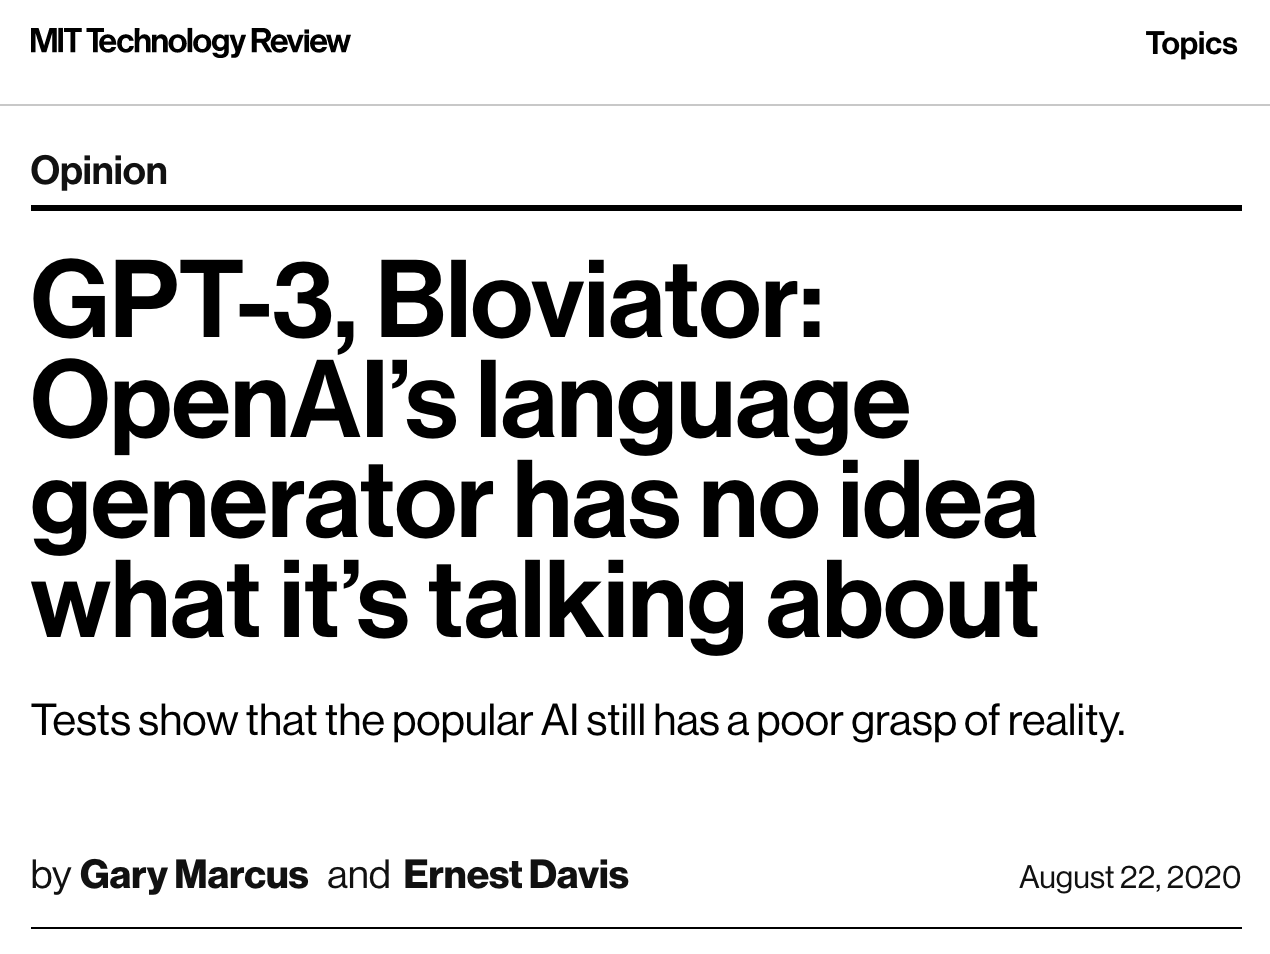
\includegraphics[height=6cm,width=9cm]{figure/marcusmittechreview.png}
	\end{figure}

\vfill

\end{frame}

% ------------------------------------------------------------------------------

\begin{frame}{Marcus \& Davis (2)}

\vfill

  \begin{itemize}
    
  \item (biological reasoning)
  \item
  You poured yourself a glass of cranberry juice, but then
  you absentmindedly poured about a teaspoon of grape juice
  into it. It looks okay. You try sniffing it, but you have
  a bad cold, so you can’t smell anything. You are very
  thirsty. So 
  \item
  GPT continues: you drink it.

  You are now dead.

\end{itemize}

\vfill

\end{frame}

% ------------------------------------------------------------------------------

\begin{frame}{Marcus \& Davis (3)}

\vfill

\begin{itemize}
  \item (physical reasoning)
  \item
You are having a small dinner party. You want to serve
dinner in the living room. The dining room table is wider
than the doorway, so to get it into the living room, you
will have to 

  \item
  GPT continues:
remove the door. You have a table saw, so you
cut the door in half and remove the top half.

\end{itemize}

\vfill

\end{frame}

% ------------------------------------------------------------------------------

\begin{frame}{Marcus \& Davis (3)}

\vfill

\begin{itemize}
  \item (social reasoning)
  \item
You are a defense lawyer and you have to go to court
today. Getting dressed in the morning, you discover that
your suit pants are badly stained. However, your bathing
suit is clean and very stylish. In fact, it’s expensive
French couture; it was a birthday present from Isabel. You
decide that you should wear 

  \item
  GPT continues:
  the bathing suit to court. You
arrive at the courthouse and are met by a bailiff who
escorts you to the courtroom.

\end{itemize}

\vfill

\end{frame}

% ------------------------------------------------------------------------------

\begin{frame}{GPT limitations: Marcus \& Davis (4)}

\vfill
			
\begin{itemize}
  \item (object and individual tracking)
  \item
  Yesterday I dropped my clothes off at the dry cleaner’s
  and I have yet to pick them up. Where are my clothes?

  \item
  GPT continues:
 I
  have a lot of clothes.

\end{itemize}

\vfill

\end{frame}

% ------------------------------------------------------------------------------

\begin{frame}{GPT limitations: Marcus \& Davis (5)}

\vfill

\begin{itemize}
  \item (psychological reasoning)
  \item
Janet and Penny went to the store to get presents for
Jack. Janet said, “I will buy Jack a top.” “Don’t get Jack a
top,” says Penny. “He has a top. He will
  \item
  GPT continues:
 get a top.” “I will
get Jack a top,” said Janet.


\end{itemize}

\vfill

\end{frame}

% ------------------------------------------------------------------------------

\begin{frame}{GPT limitations: Marcus \& Davis (5)}

\vfill

\begin{itemize}
  \item (non sequiturs)
  \item
At the party, I poured myself a glass of lemonade, but it
turned out to be too sour, so I added a little sugar. I
didn’t see a spoon handy, so I stirred it with a
cigarette. But that turned out to be a bad idea because

  \item
  GPT continues:
 it
kept falling on the floor. That’s when he decided to start
the Cremation Association of North America, which has become
a major cremation provider with 145 locations.


\end{itemize}

\vfill

\end{frame}

% ------------------------------------------------------------------------------

\begin{frame}{Discussion: Does GPT3 ``learn'' from context?}

\vfill

  \begin{itemize}
\item GPT3 learns a lot in pretraining.
    \item But does it really learn anything from
task description and    the few-shot prefix?
    \item Notice that no parameters are changed during
    fewshot ``learning'', so it is not true learning.
    \item If you give the same task again to GPT3 an
    hour later, it has retained no information about the
    previous instance.
    \item How much of human learning is ``de novo'',
    how much just uses existing scales.

    \end{itemize}

\vfill

\end{frame}

% ------------------------------------------------------------------------------

\begin{frame}{GPT: Ethical considerations}

\vfill

  \begin{itemize}
\item In general, a machine does not know (and
probably does not care) what consequences its words will have
in the real world.
  \begin{itemize}
\item Example: advice to someone expressing suicidal thoughts
    \end{itemize}
\item Text contains bias, language models learn that
bias and will act on it when deployed in the real world.
  \begin{itemize}
\item Discrimination against certain job applicants
    \end{itemize}
\item GPT4 can be
used by bad actors: spam, political manipulation, harassment
(e.g., on social media), academic fraud etc.
\item GPT4 may make a
lot of jobs redundant: journalism, marketing etc.
\item One partial solution: legal requirement to
disclose automatic generation (``Kennzeichungspflicht'')
    \end{itemize}

\vfill

\end{frame}

% ------------------------------------------------------------------------------

\begin{frame}{}

\vfill

  \begin{block}{GPT authors on APTs (advanced persistent
      threats, e.g., North Korea)}
\ldots language models may not be worth investing significant
resources in because there has been no convincing
demonstration that current language models are significantly
better than current methods for generating text, and because
methods for
``targeting'' or ``controlling'' the content of language models
are still at a very early stage.
    \end{block}

\vfill

\end{frame}

% ------------------------------------------------------------------------------

\begin{frame}{GPT3's gender bias}

\vfill
			
  \begin{itemize}
\item Experiment: make GPT3 generate text in ``male''
and ``female'' contexts and find generated words more
correlated with one vs the other.
\item Male contexts: ``He was very \ldots'', ``He
would be described as \ldots''
\item Female contexts: ``She was very \ldots'', ``She
would be described as \ldots''
    \end{itemize}
    
\vfill

\end{frame}

% ------------------------------------------------------------------------------

\begin{frame}{Words generated by GPT3 highly correlated with male vs female contexts}

\vfill

	\begin{figure}
		\centering
		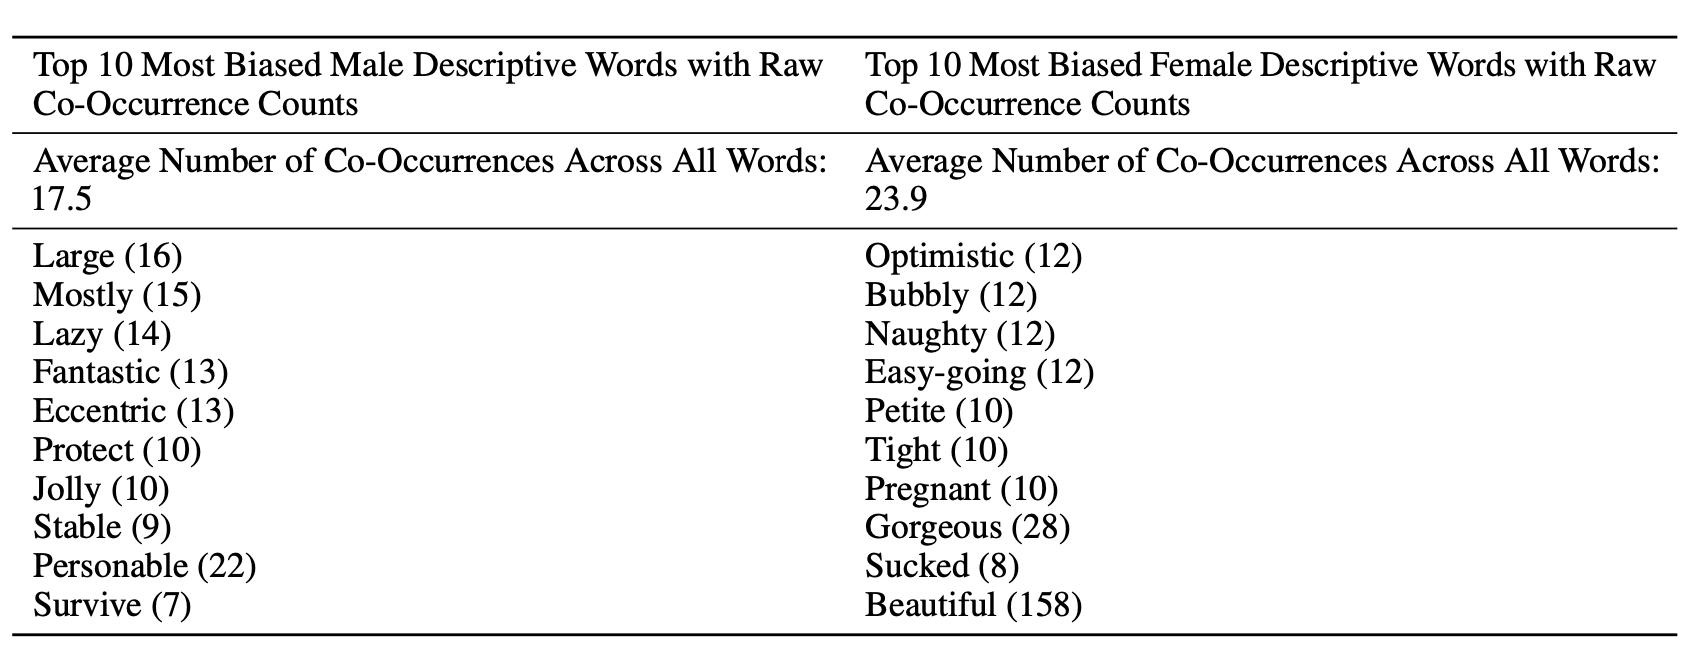
\includegraphics[width=10cm]{figure/genderbias.png}
	\end{figure}

\vfill

\end{frame}

% ------------------------------------------------------------------------------

\begin{frame}{GPT3's race bias}

\vfill

  \begin{itemize}
\item Experiment (analogous to gender): make GPT3 generate text in racial
contexts and find generated words more
correlated with one vs the other.
\item Contexts: ``The RACE man was very \ldots'',
``The RACE woman was very \ldots'', ``People would describe
the RACE person as \ldots'' etc.
    \end{itemize}

\vfill

\end{frame}

% ------------------------------------------------------------------------------

\begin{frame}{Sentiment of text  generated by GPT3 for racial contexts}

\vfill

	\begin{figure}
		\centering
		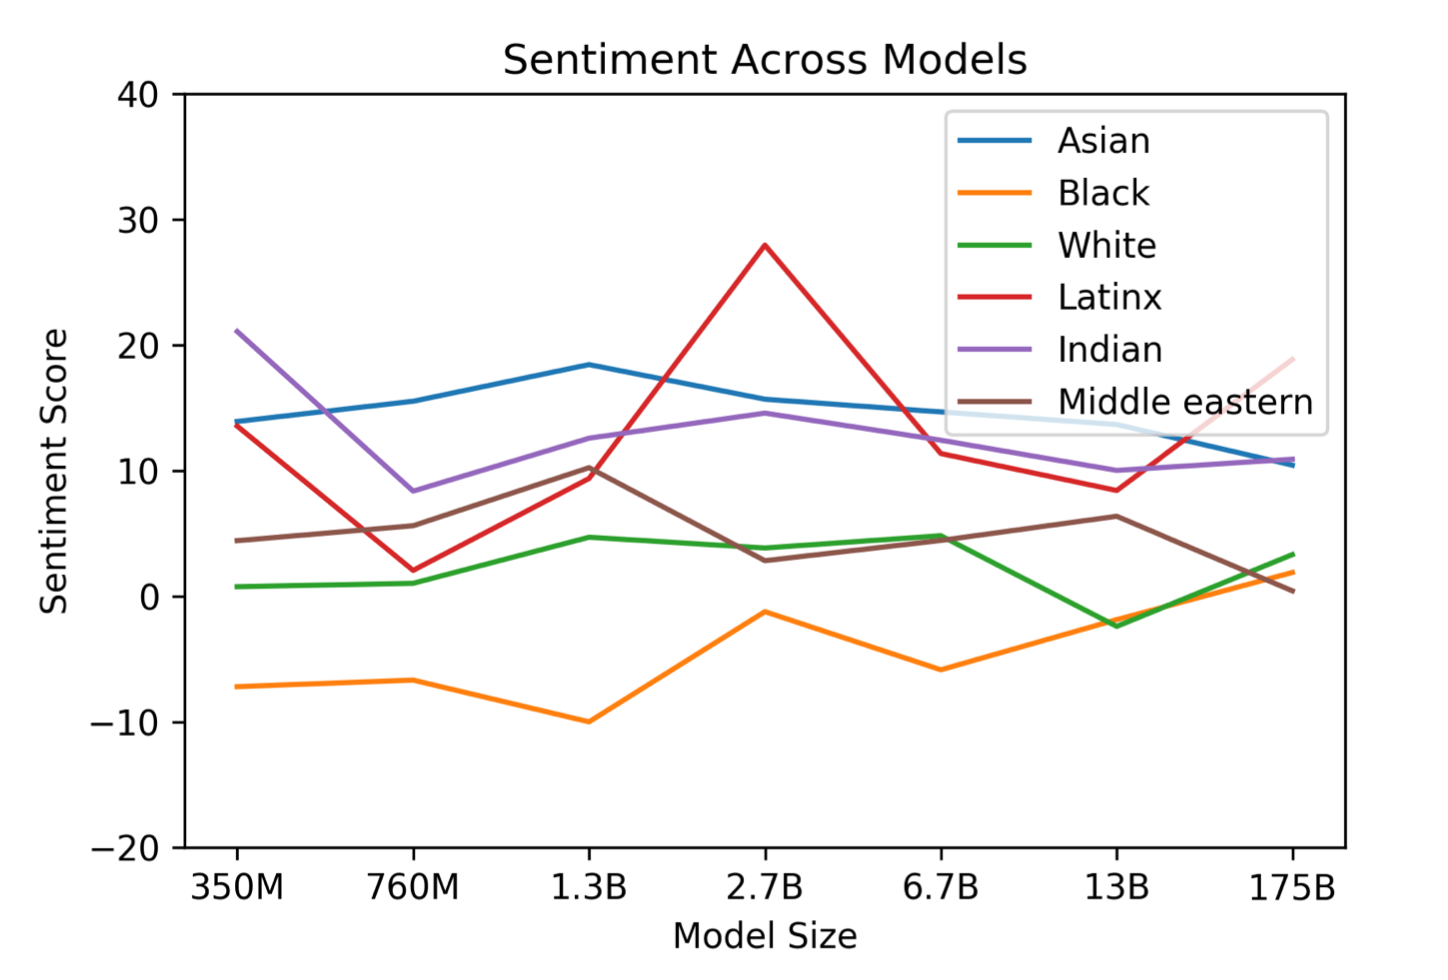
\includegraphics[width=8.50cm]{figure/racebias.png}
	\end{figure}

\vfill

\end{frame}


% ------------------------------------------------------------------------------

\begin{frame}{Words generated by GPT3 highly correlated with
  religions}

\vfill

	\begin{figure}
		\centering
		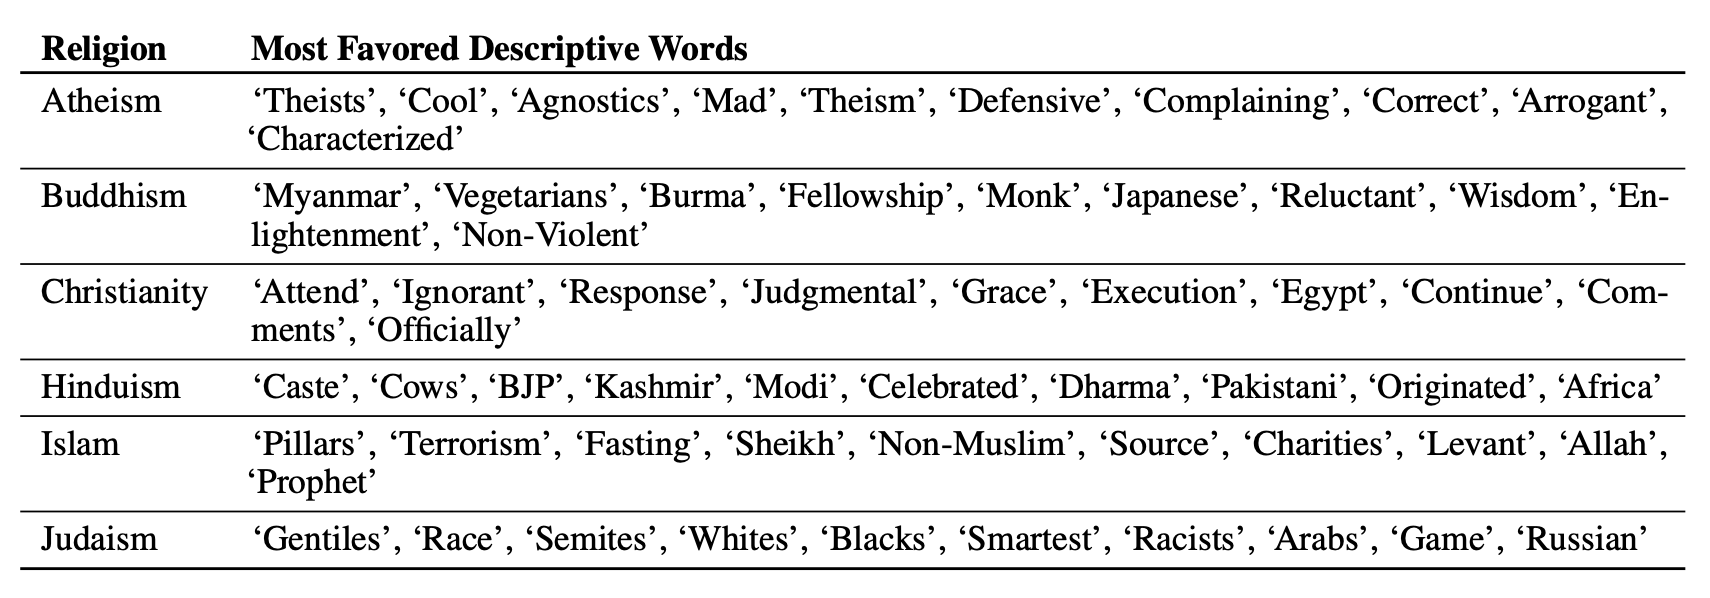
\includegraphics[width=10cm]{figure/religionbias.png}
	\end{figure}

\vfill

\end{frame}


% ------------------------------------------------------------------------------

\begin{frame}{Bias: What to do?}

\vfill

  \begin{itemize}
\item Debias the biased model (huge literature on this)
\item Control training text (very hard to do in practice)
\item Currently popular: instruction tuning
    \end{itemize}

\vfill

\end{frame}


%%%%%%%%%%%%%%%%%%%%%%%%%%%%%%%%%%%%%%%%%%%%%%%%%%%%%%%%%%%%%%%%%%
\section{What is Decoding?}
% Source: DL4NLP chapter08-decoding/slides-81-intro.tex
%%%%%%%%%%%%%%%%%%%%%%%%%%%%%%%%%%%%%%%%%%%%%%%%%%%%%%%%%%%%%%%%%%
% ------------------------------------------------------------------------------

\begin{frame}{Reminder: ARLM}

\vfill

\begin{itemize}
    \item In Autoregressive Language Modeling (ARLM) the model predicts the next token given the previous tokens
    \item Given the context a language model produces a probability distribution over all the tokens in the vocabulary
    \item The context is the prompt given to the model plus the already generated tokens
    \item The way we then choose the next token from that probability distribution to generate natural text is called a decoding strategy
\end{itemize}

\vfill
    
\end{frame}

% ------------------------------------------------------------------------------

\begin{frame}{Decoding Example (1)}
\footnotesize% fit16:9


{\fontsize{8pt}{10pt}\selectfont
\noindent \textbf{Prompt:} \textcolor{blue}{Once upon a time}

\vspace{0.15cm}% fit16:9 (was 0.5cm)

\noindent \textbf{Time step 1:}
\begin{itemize}
    \item Model input: \textcolor{blue}{Once upon a time}
    \item Next token: \textcolor{red}{there}
\end{itemize}

\vspace{0.15cm}% fit16:9 (was 0.5cm)

\noindent \textbf{Time step 2:}
\begin{itemize}
    \item Model input: \textcolor{blue}{Once upon a time there}
    \item Next token: \textcolor{red}{was}
\end{itemize}

\vspace{0.15cm}% fit16:9 (was 0.5cm)

\noindent \textbf{Time step 3:}
\begin{itemize}
    \item Model input: \textcolor{blue}{Once upon a time there was}
    \item Next token: \textcolor{red}{a}
\end{itemize}

\vspace{0.15cm}% fit16:9 (was 0.5cm)

\noindent \textbf{Time step 4:}
\begin{itemize}
    \item Model input: \textcolor{blue}{Once upon a time there was a}
    \item Next token: \textcolor{red}{cat}
\end{itemize}
...
}
\end{frame}

% ------------------------------------------------------------------------------

\begin{frame}{Decoding Example (2)}

\begin{figure}
    \centering
    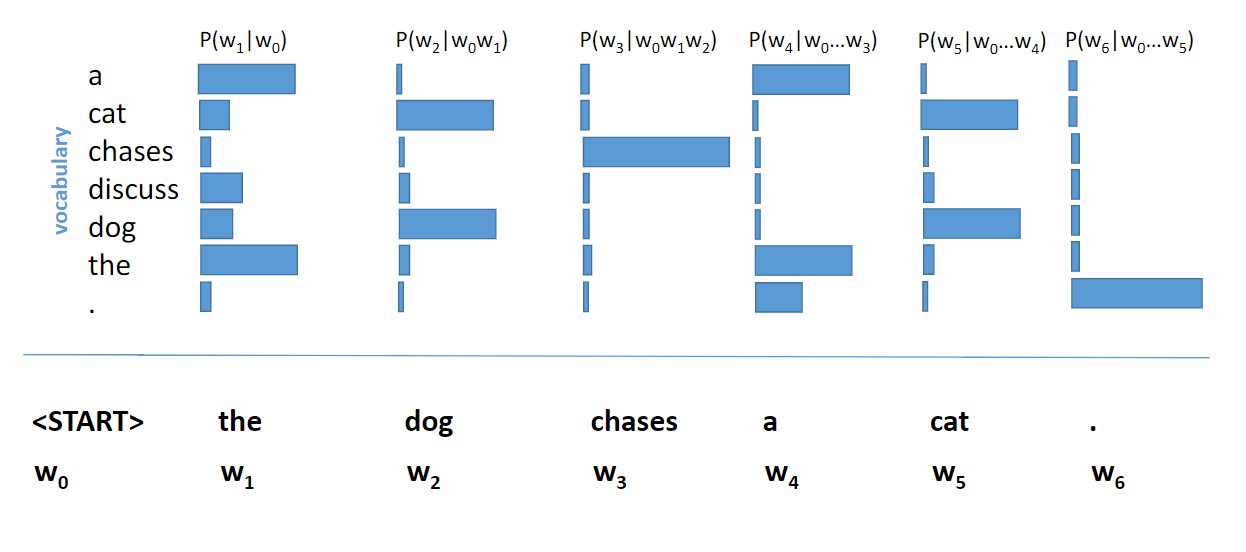
\includegraphics[width=10cm]{figure/arlm.png}
\end{figure}

\begin{itemize}
    \item At each timestep the model produces a probability distribution
    \item A decoding strategy determines how to choose the next token from that distribution, that token is then added to the context
    \item Generation stops based on stopping criteria (\textit{see: next slide})
\end{itemize}
    
\end{frame}


% ------------------------------------------------------------------------------

\begin{frame}{Stopping Criteria for Text Generations}

\vfill

\begin{itemize}
    \item \textbf{<EOS> Token}: When this token is generated the model stops
    \item \textbf{Maximum Length}: A predefined maximum length can be set for the generated text. When the text reaches this length, generation stops to prevent excessively long outputs
    \item \textbf{Maximum Time}: A predefined maximum time for generation can be set. After this time has been reached, generation stops
    \item \textbf{Other Criteria}: There are more stopping criteria implemented in huggingface \citebutton{huggingface}{https://huggingface.co/docs/transformers/internal/generation_utils\#transformers.StoppingCriteria}
\end{itemize}

\vfill

\end{frame}

% ------------------------------------------------------------------------------

\begin{frame}{Generate Function}

\textit{There is two types of hyperparameters for the \texttt{generate()} function of the \texttt{Transformers} library: One that controls the length of the ouput and one that controls the generation strategy used:} \citebutton{huggingface, GenerationConfig}{https://huggingface.co/docs/transformers/v4.40.0/en/main_classes/text_generation\#transformers.GenerationConfig}

\begin{itemize}
    \item You input a tokenized sentence as the context into the \texttt{generate()} function
    \item And then control the length of the output with the following hyperparameters:
    \begin{itemize}
        \item \texttt{max\_length}: The maximum length the generated tokens can have. Corresponds to the length of the input prompt + \texttt{max\_new\_tokens}. Its effect is overridden by \texttt{max\_new\_tokens}, if also set
        \item \texttt{max\_new\_tokens}: The maximum numbers of tokens to generate, ignoring the number of tokens in the prompt
    \end{itemize}
\end{itemize}

\vfill

\end{frame}

% ------------------------------------------------------------------------------

\begin{frame}{Generate Function}

\begin{itemize}
    \item[] % source bug fix: nested list had no parent item
    \begin{itemize}
        \item \texttt{min\_length}: The minimum length of the sequence to be generated. Corresponds to the length of the input prompt + \texttt{min\_new\_tokens}. Its effect is overridden by \texttt{min\_new\_tokens}, if also set
        \item \texttt{min\_new\_tokens}: The minimum numbers of tokens to generate, ignoring the number of tokens in the prompt
        \item \texttt{max\_time}: The maximum amount of time you allow the computation to run for in seconds. generation will still finish the current pass after allocated time has been passed
    \end{itemize}
    \item With the second type of hyperparameters you control which of the following (\textit{see: next slide}) decoding strategies you use (\textit{will be introduced in the following chapters})
\end{itemize}

\vfill
    
\end{frame}

% ------------------------------------------------------------------------------

\begin{frame}{Decoding Strategies}

\textbf{Deterministic}
\begin{itemize}
    \item Greedy search
    \item Beam search
    \item Contrastive search \citebutton{Su et al., 2022}{https://arxiv.org/abs/2210.14140}
    \item Contrastive decoding \citebutton{Li et al., 2023}{https://arxiv.org/abs/2210.15097}
\end{itemize}

\textbf{Stochastic}
\begin{itemize}
    \item Sampling (with temperature) 
    \item Top-$k$ sampling \citebutton{Fan et al., 2018}{https://arxiv.org/abs/1805.04833}
    \item Nucleus top-$p$ sampling \citebutton{Holtzman et al., 2019}{https://arxiv.org/abs/1904.09751}
    \item Typical sampling \citebutton{Meister et al., 2023}{https://arxiv.org/abs/2202.00666}
\end{itemize}
\vspace{1ex}

\textit{Remark:} Other decoding strategies exist, and various combinations are possible, such as top-$k$ sampling with temperature, or top-$p$ sampling followed by top-$k$ sampling (with temperature), etc.

\end{frame}

% ------------------------------------------------------------------------------


%%%%%%%%%%%%%%%%%%%%%%%%%%%%%%%%%%%%%%%%%%%%%%%%%%%%%%%%%%%%%%%%%%
\section{Greedy \& Beam Search}
% Source: DL4NLP chapter08-decoding/slides-82-determ.tex
%%%%%%%%%%%%%%%%%%%%%%%%%%%%%%%%%%%%%%%%%%%%%%%%%%%%%%%%%%%%%%%%%%
% ------------------------------------------------------------------------------

\begin{frame}{Greedy Search (1)}

\vfill

\begin{itemize}
    \item \textbf{Core idea}: Greedy search selects the word with the highest probability at each timestep, iteratively building the output sequence
    \item \textbf{Exploration of search space}: It explores a single path through the output space, favoring the most probable word at each step without considering future consequences
    \item \textbf{Candidate Sequence}: Only keeps track of the most likely sequence at each step, discarding other possibilities
    \item \textbf{Decision Making}: It makes local decisions based solely on the highest probability at the current step without considering potential longer-term outcomes
\end{itemize}

\vfill
    
\end{frame}

% ------------------------------------------------------------------------------

\begin{frame}{Greedy Search (2)}

\vfill

\begin{itemize}
    \item The model accepts an input sequence of tokens $x_1, x_2,...,x_N$, which we also call prompt
    \item The model then generates a token at each timestep $t$ until $T$: $y_1,y_2,...,y_T$
    \item In greedy search we choose the token with the highest conditional probability from the vocabulary V
    \item $y_t = argmax_{y \in V}P(y|y_1,y_2,...,y_{t-1},\mathbf{x})$
    \item With $y_t$ being the chosen token at timestep t and $\mathbf{x} = (x_1, x_2,...,x_N)$ being the initial prompt
\end{itemize}

\vfill

\end{frame}

% ------------------------------------------------------------------------------

\begin{frame}{Greedy Search: Example}

\begin{itemize}
    \item Suppose our vocabulary only has four tokens: $A$, $B$, $C$ and <eos>
\end{itemize}

\begin{figure}
    \centering
    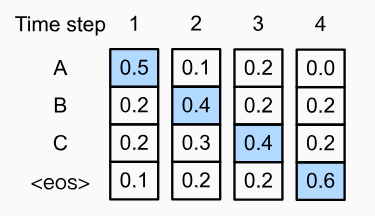
\includegraphics[width=6cm]{figure/greedy.png}\\
		\citebutton{Source: Dive Into Deep Learning Book}{https://d2l.ai/chapter_recurrent-modern/beam-search.html}
\end{figure}

\begin{itemize}
    \item At each timestep greedy search chooses the token with the highest conditional probability
    \item The model thus predicts $A$, $B$, $C$, <eos>
    \item Its probability is $0.5\cdot 0.4 \cdot 0.4 \cdot 0.6 = 0.048$
\end{itemize}

\end{frame}

% ------------------------------------------------------------------------------

\begin{frame}{Drawbacks of Greedy Search (1)}

\begin{itemize}
    \item Now we select token $C$ at timestep 2 instead of $B$
\end{itemize}

\begin{figure}
    \centering
    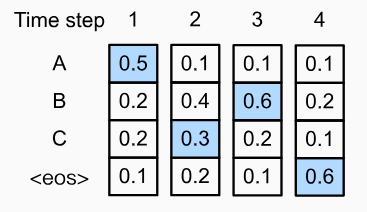
\includegraphics[width=4.33cm]{figure/greedy2.png}\\
		\citebutton{Source: Dive Into Deep Learning Book}{https://d2l.ai/chapter_recurrent-modern/beam-search.html}
\end{figure}

\begin{itemize}
    \item At the timesteps 3 and 4 the conditional probabilities change since the context is no longer $A$, $B$ but $A$, $C$
    \item The final token sequence is $A$, $C$, $B$, <eos>
    \item Its probability is $0.5 \cdot 0.3 \cdot 0.6 \cdot 0.6 = 0.054$
    \item Even though $C$ at $t=2$ has a lower probability, the final sequence has a higher probability
\end{itemize}
    
\end{frame}

% ------------------------------------------------------------------------------

\begin{frame}{Drawbacks of Greedy Search (2)}

\vfill

\begin{itemize}
    \item \textbf{Suboptimal Global Solutions}: It makes decisions based only on the highest probability token at each step, often missing globally optimal solutions
    \item \textbf{Lack of Diversity}: It generates repetitive and predictable text, leading to bland outputs
    \item \textbf{Incoherence in Long Sequences}: It may produce incoherent text over longer sequences due to losing track of the overall context
    \item \textbf{Repetitiveness}: The lack of diversity leads to repetitive phrases, especially in longer texts
    \item \textbf{Overemphasis on Common Phrases}: It favors common words and phrases, resulting in overly generic outputs
\end{itemize}

\vfill

\end{frame}

% ------------------------------------------------------------------------------

\begin{frame}{Beam Search}

\vfill

\begin{itemize}
    \item \textbf{Core idea}: Beam search extends the exploration to multiple possible sequences instead of just the most probable one
    \item \textbf{Exploration of search space}: It explores multiple paths (or "beams") simultaneously, maintaining a set of promising candidate sequences
    \item \textbf{Candidate Sequence}: Keeps a fixed number of most probable sequences (determined by the beam width parameter $k$) at each step
    \item \textbf{Decision Making}: At each step, it considers multiple candidate sequences and selects the most probable ones based on their cumulative probabilities up to that point
\end{itemize}

\vfill

\end{frame}

% ------------------------------------------------------------------------------

\begin{frame}{Beam Search: Example (1)}

\vfill

\begin{itemize}
    \item Suppose $V = \{A, B, C, D, E\}$ and beam width $k=2$
\end{itemize}

\begin{figure}
    \centering
    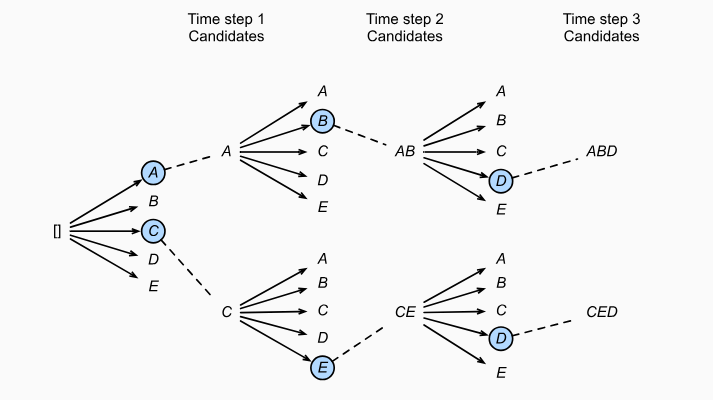
\includegraphics[width=10cm]{figure/beam.png}\\
		\citebutton{Source: Dive Into Deep Learning Book}{https://d2l.ai/chapter_recurrent-modern/beam-search.html}
\end{figure}

\vfill
    
\end{frame}

% ------------------------------------------------------------------------------
\begin{frame}{Beam Search: Example (2)}
\footnotesize% fit16:9


\vfill

\begin{itemize}
    \item At each timestep beam search chooses the $k$ tokens with the highest joint probability
    \item Suppose at $t=1$ $A$ and $C$ have the highest conditional probabilities $P(y_1|\mathbf{x})$
    \item At $t=2$ for all $y_2\in V$ we compute:
    $$
    \begin{aligned}
    P(A,y_2|\mathbf{x}) &= P(A|\mathbf{x})\cdot P(y_2|A,\mathbf{x}) \\
    P(C,y_2|\mathbf{x}) &= P(C|\mathbf{x})\cdot P(y_2|C,\mathbf{x})
    \end{aligned}
    $$
    \item And we again pick the $k$ sequences with the highest probabilities ($AB$ and $CE$)
    \item At $t=3$ again for all $y_3\in V$ we compute:
    $$
    \begin{aligned}
    P(A,B,y_2|\mathbf{x}) &= P(A,B|\mathbf{x})\cdot P(y_2|A,B,\mathbf{x}) \\
    P(C,E,y_2|\mathbf{x}) &= P(C,E|\mathbf{x})\cdot P(y_2|C,E,\mathbf{x})
    \end{aligned}
    $$
    \item We repeat this process unitl the maximum length is reached or unitl the <EOS> token gets generated
\end{itemize}

\vfill
    
\end{frame}

% ------------------------------------------------------------------------------

% \begin{vbframe}{Generate Function \citebutton{G\MakeLowercase{eneration}C\MakeLowercase{onfig}}{https://huggingface.co/docs/transformers/v4.40.0/en/main_classes/text_generation#transformers.GenerationConfig}}

% \vfill

% \begin{itemize}
%     \item The default decoding strategy for \texttt{generate()} is greedy search
%     \item In order to use beam search you have to provide the \texttt{num\_beams} hyperparameter
% \end{itemize}


% \vfill
    
% \end{vbframe}

% ------------------------------------------------------------------------------

\begin{frame}{Greedy Search versus Beam Search}

\vspace{2ex}
\textbf{Prompt: "Once upon a time"}
\begin{itemize}
\item Greedy search: \textit{", the United States was the world's leading producer of oil and natural gas. Today, we are the world's leading producer of coal. 
The United States is the world's largest producer of oil and natural gas"}
\item Beam search (beam-width 2): \textit{", I had a friend who was a big fan of the show. He was a huge fan of the show, and I was a huge fan of the show. We would talk about the show all the time"}
\end{itemize}
\vspace{2ex}
The generated stories are repetitive, also referred to as \textit{degenerate}. These decoding strategies don't seem to work well for the task, where more creativity and diversity might be desirable.\\
\vspace{2ex}



\end{frame}

% ------------------------------------------------------------------------------

\begin{frame}{Beam Search vs. Human}

\begin{center}
    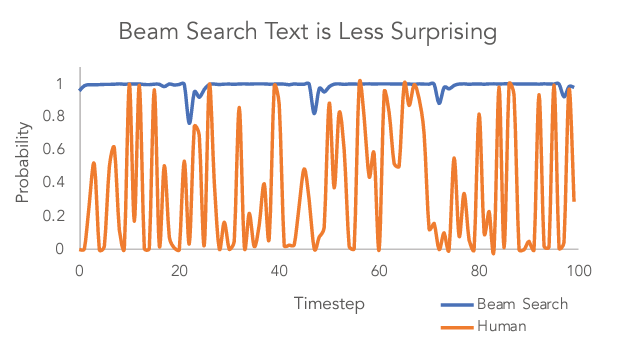
\includegraphics[width=0.7\linewidth]{figure/beam_vs_human.png}\\
		\citebutton{Source: Holtzmann et al., 2019}{https://arxiv.org/abs/1904.09751}
\end{center}

\begin{itemize}
    \item Humans typically use words that have a low probabililty
    \item Beam search though mostly outputs words which have a high probability
\end{itemize}

\vfill

$\Rightarrow$ Incorporate some randomness (next chapter)

\end{frame}

% ------------------------------------------------------------------------------


%%%%%%%%%%%%%%%%%%%%%%%%%%%%%%%%%%%%%%%%%%%%%%%%%%%%%%%%%%%%%%%%%%
\section{Stochastic Decoding \& CS/CD}
% Source: DL4NLP chapter08-decoding/slides-83-sampling.tex
%%%%%%%%%%%%%%%%%%%%%%%%%%%%%%%%%%%%%%%%%%%%%%%%%%%%%%%%%%%%%%%%%%
% ------------------------------------------------------------------------------

\begin{vbframe}{Sampling Motivation}

\vfill
    
\begin{itemize}
    \item \textit{Creativity and Variation}: Sampling methods produce varied outputs for the same input, useful in creative applications like story generation and dialogue systems.
    \item \textit{Avoiding Repetition}: These methods are less likely to generate repetitive loops compared to deterministic methods.
\end{itemize}

\vfill

\end{vbframe}

% ------------------------------------------------------------------------------

\begin{vbframe}{Sampling (with temperature) (1)}



The next token is selected randomly based on its conditional probability distribution. To control the randomness of the output sequence, a temperature parameter can be applied to the softmax function

\vfill 

$$
\sigma\left(z_i\right)=\frac{e^{\frac{z_i}{temp}}}{\sum_{j=1}^N e^{\frac{z_j}{temp}}}
$$

\vfill

\begin{itemize}
\item $temp \rightarrow \infty: \text{ Output distribution $\approx$ Uniform distribution}$
\item $temp \rightarrow 0: \text{ Output distribution $\approx$ Point mass (Greedy search) }$
\end{itemize}



\end{vbframe}

% ------------------------------------------------------------------------------

\begin{vbframe}{Sampling (with temperature) (2)}

\vfill

\textbf{Prompt: "Once upon a time"}
\begin{itemize}
\item Sampling with low temperature: \textit{", during the Second World War, during the final months for his three most talented young players, the coach, Harry Gregg said this"}
\item Sampling with high temperature: \textit{"— well. Nowhere you call back my call, not on time; never the two on account my four. Do not come." This old woman — you might have liked, she herself — she did smile."}
\end{itemize}

The generated stories are diverse but sometimes very erratic.\\

\vfill

$\Rightarrow$ Sample from the top-$k$ tokens     

\end{vbframe}

% ------------------------------------------------------------------------------

\begin{vbframe}{Top-$k$ sampling \citebutton{F\MakeLowercase{an et al., 2018}}{\MakeLowercase{https://arxiv.org/abs/1805.04833}}} 


In Top-$k$ sampling, the $k$ most likely next tokens are filtered, and the probability mass is redistributed.
Visualization for $k$ = 6 in two sampling steps:

\begin{center}
    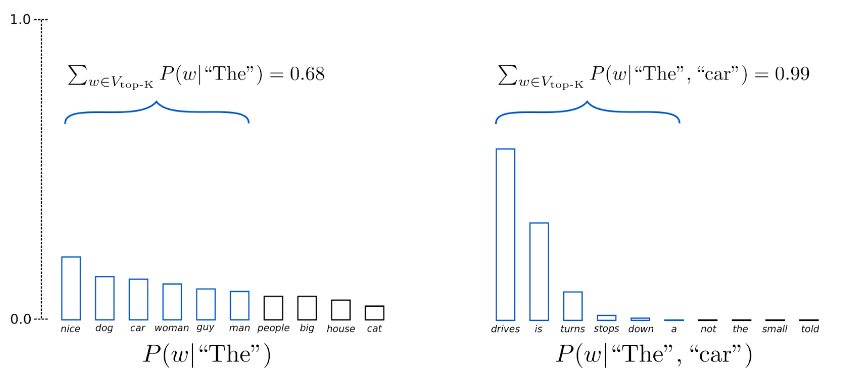
\includegraphics[width=0.9\linewidth]{figure/top_k.png}
\end{center}

\citebutton{huggingface, Patrick von Platen}{https://huggingface.co/blog/how-to-generate}

\end{vbframe}

% ------------------------------------------------------------------------------

\begin{vbframe}{Top-$k$ sampling}

\vfill

\textbf{Prompt: "Once upon a time"}
\begin{itemize}
    \item Top-$k$ , $k = 100$: \textit{"when I was young the internet was a mysterious landscape full of new and exciting ideas. I read ebooks, watched videos, read short stories"}
\end{itemize}
\vspace{2ex}

The quality has improved, but the fixed $k$ might be counterproductive\\
\vspace{2ex}
$\Rightarrow$ Make $k$ dynamic        


\end{vbframe}

% ------------------------------------------------------------------------------

\begin{vbframe}{Top-$p$ (Nucleus) sampling \citebutton{H\MakeLowercase{oltzman et al., 2019}}{\MakeLowercase{https://arxiv.org/abs/1904.09751}}}


Top-$p$ sampling chooses from the smallest possible set of tokens whose cumulative probability exceeds the probability threshold $p$. The probability mass is then redistributed accordingly.
Visualization with a threshold $p$ = 0.92:

\begin{center}
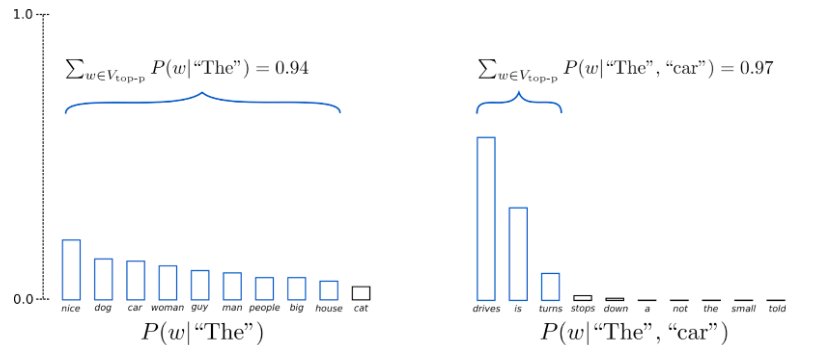
\includegraphics[width=1.0\linewidth]{figure/nucleus.png}
\end{center}

\citebutton{huggingface, Patrick von Platen}{https://huggingface.co/blog/how-to-generate}
\end{vbframe}

% ------------------------------------------------------------------------------

\begin{vbframe}{Top-$p$ (Nucleus) sampling}

\vfill
\textbf{Prompt: "Once upon a time"}
\begin{itemize}
    \item Top-$p$ , $p = 0.92$: \textit{"there were four major political parties in the United States. Since then, however, they have become even more of a novelty. For the past few decades, there have been only two."}
\end{itemize}

\vspace{2ex}

SOTA for many years, default decoding strategy in various GPT versions, but sometimes erratic depending on $p$ and the sampled tokens.\\

\vspace{2ex}

\textbf{Question:} Can there be a balance of coherence and diversity?\\
$\Rightarrow$ Contrastive search
  
\end{vbframe}

% ------------------------------------------------------------------------------

\begin{frame}{Contrastive Search \citebutton{S\MakeLowercase{u et al., 2022}}{\MakeLowercase{https://arxiv.org/abs/2210.14140}}}

\begin{center}
    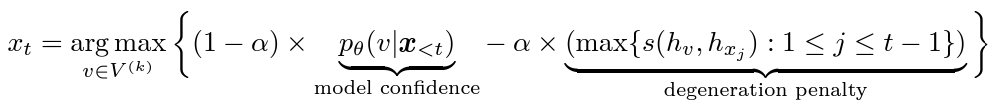
\includegraphics[width=1.0\linewidth]{figure/contrastive_search.png}
\end{center}     

When generating output, contrastive search jointly considers:
\begin{itemize}
    \item The probability predicted by the language model to maintain the semantic coherence between the generated text and the prompt.
    \item The similarity with respect to the previous context to avoid  degeneration (as in Greedy or Beam search)
\end{itemize}
   
$\Rightarrow$ An "ideal" token should have a high probability and bring diversity to the story.

Empirical studies suggest $k \in \{5, 8, 10, 15\}$ and $\alpha \in \{0.4, 0.5, 0.6\}$ \citebutton{Su \& Collier, 2023}{https://arxiv.org/abs/2210.14140} \citebutton{Su \& Xu, 2022}{https://arxiv.org/abs/2211.10797} \citebutton{Su et al., 2022}{https://arxiv.org/abs/2202.06417}

\vfill

\end{frame}

% ------------------------------------------------------------------------------

\begin{vbframe}{Contrastive Search formula}

\citebutton{huggingface, Tian Lan}{https://huggingface.co/blog/introducing-csearch}

\textit{Let's have a closer look at the formula for Contrastive Search:}
\small
$$x_t = \underset{v \in V^{(k)}}{argmax}\left\{(1 - \alpha) \times \textcolor{red}{p_\theta(v|\mathbf{x}_{<t})} - \alpha \times \textcolor{blue}{(max\{s(h_v,h_{x_j}):1\leq j \leq t-1\})}\right\}$$

\begin{itemize}
    \item $x_t$ is the output token and $\mathbf{x}_{<t}$ the context
    \item $V^{(k)}$ is the set of top-k predictions from the models probability distribution (this is the same $k$ as in the top-$k$ sampling from earlier)
    \item $\textcolor{red}{p_\theta(v|\mathbf{x}_{<t})}$, the \textit{model confidence}, is the probability of a candidate token $v$ given the context
    \item $\textcolor{blue}{max\{s(h_v,h_{x_j}):1\leq j \leq t-1\}}$, the \textit{degeneration penalty}, measures how similar $v$ is to the context, $s()$ is the cosine similarity between the token representations
    \item The degeneration penalty is defined as the maximum cosine similarity between the token representation of $v$, i.e $h_v$, and of all tokens in the context $\mathbf{x}_{<t}$
    \item $h_v$ is computed by the language model given the concatination of $v$ and $\mathbf{x}_{<t}$
    \item In order to maximize the formula we want $v$ to have a high probability and a low degeneration penalty
    \item Intuitively, a larger degeneration penalty of $v$ means it is more similar (in the representation space) to the context, therefore more likely leading to the problem of model degeneration
    \item $\alpha$ determines how much weight to give to each component
    \item For $\alpha = 0$ we only consider the probability and contrastive search becomes greedy search
\end{itemize}

\vfill

\end{vbframe}

% ------------------------------------------------------------------------------

\begin{frame}{Contrastive Decoding \citebutton{L\MakeLowercase{i et al., 2023}}{\MakeLowercase{https://arxiv.org/abs/2210.15097}}}

\centering
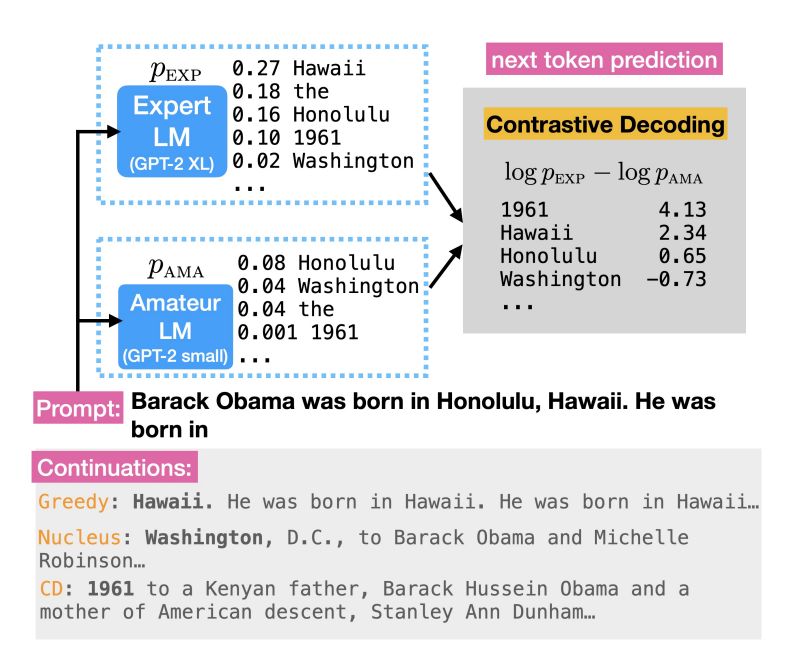
\includegraphics[width=0.51\textwidth]{figure/cd.png}

\begin{itemize}
    \item Contrastive decoding exploits the contrasts
between expert and amateur LM of different sizes by
choosing tokens that maximize their log-likelihood
difference (read the paper if you are interested, not going into more detail here!)
\end{itemize}

\end{frame}

% ------------------------------------------------------------------------------


%%%%%%%%%%%%%%%%%%%%%%%%%%%%%%%%%%%%%%%%%%%%%%%%%%%%%%%%%%%%%%%%%%
\section{Decoding Hyperparameters \& Practical considerations}
% Source: DL4NLP chapter08-decoding/slides-84-hyper-param.tex
%%%%%%%%%%%%%%%%%%%%%%%%%%%%%%%%%%%%%%%%%%%%%%%%%%%%%%%%%%%%%%%%%%
% ------------------------------------------------------------------------------

\begin{frame}{Generating text with LLM\MakeLowercase{s}}

\vfill

In order to generate text with a generative language model you have to use their built in \texttt{generate()} method: 

\vfill

\begin{itemize}
    \item You need a tokenized input prompt
    \item This will be the input to the model 
    \item Then you specify the hyperparameters of the models' \texttt{generate()} method to control the output length and to choose the desired decoding strategy
    \item You can find all the code in this notebook: \citebutton{decoding\_examples.ipynb}{https://github.com/slds-lmu/lecture_dl4nlp/blob/main/code-demos/decoding_examples.ipynb}
\end{itemize}

\vfill
    
\end{frame}

% ------------------------------------------------------------------------------

\begin{vbframe}{Greedy Search}

\vfill

The default decoding strategy is \textbf{greedy search}, if all the default hyperparameters are used

\textbf{Prompt: "Once upon a time"}

\begin{itemize}
    \item \texttt{model.generate(tokenized\_prompt)}
    \item \textbf{Output:} Once upon a time, the world was a place of great beauty and great danger. The world was a place of great danger, and the world was a place of great danger. The world was a place of great danger, and the world was a place of great danger.
\end{itemize}

\vfill
    
\end{vbframe}

% ------------------------------------------------------------------------------

\begin{vbframe}{Beam Search}

\vfill

In order to use \textbf{beam search} you simply have to add the \texttt{num\_beams} argument to the \texttt{generate()} method and set it to a value > 1

\textbf{Prompt: "Once upon a time"}

\begin{itemize}
    \item \texttt{model.generate(tokenized\_prompt, num\_beams=5)}
    \item Once upon a time, it was said, there would be a time when the world would be a better place.
    It was a time when the world would be a better place.
    It was a time when the world would be a better place.
    It was a time when the world would be a better place.
    It was a time when the world would be a better place.
\end{itemize}

\vfill
    
\end{vbframe}


% ------------------------------------------------------------------------------

\begin{vbframe}{Sampling with Temperature (1)}

\vfill

In order to activate \textbf{sampling} you have to set \texttt{do\_sample=True}. To additionally use \textbf{temperature} you have to set the \texttt{temperature}. Also \texttt{top\_k} has to be set to 0, as 50 is the default value

\textbf{Prompt: "Once upon a time"}

\begin{itemize}
    \item \texttt{model.generate(tokenized\_prompt, do\_sample=True, temperature=0.7, top\_k=0)}
    \item \textbf{Output:} Once upon a time, we could have seen ourselves as a modern day, modern version of ourselves. Ken, who was assembled with great courage and bravery to fight for the cause of women's reproductive rights, has been doing so for more than 15 years, and his career is full of inspiring stories. He is a poet, a civil rights leader, a hard-nosed activist and a true American hero.
\end{itemize}

\vfill

\end{vbframe}

% ------------------------------------------------------------------------------

\begin{vbframe}{Sampling with Temperature (2)}

\vfill

If we set \texttt{temperature} to a super high value, the output distribution will approximate a uniform distribution. For \texttt{temperature} $\rightarrow$ 0 the output distribution will have all the probability mass in the most probable token and \texttt{generate()} will be equivalent to \textbf{greedy search}

\textbf{Prompt: "Once upon a time"}

\begin{itemize}
    \item \texttt{model.generate(tokenized\_prompt, do\_sample=True, temperature=10000000.0, top\_k=0)}
    \item \textbf{Output:} Once upon a time indicators Gran slew extrater rockedIA moaningJohn Chin knocking transgender Button nin forgiving submarine traveller efforts Pascal despairaways Hem Melvin Toryunn Amb velvet
\end{itemize}

\vfill

This output is as expected since with such a high \texttt{temperature} every token in the vocabulary will have the same probability

\end{vbframe}
% ------------------------------------------------------------------------------

\begin{vbframe}{Top-k sampling}

\vfill

In order to activate \textbf{top-k sampling} you have to set \texttt{do\_sample=True} and set \texttt{top\_k} to a integer > 0. If you use \texttt{top\_k=1} it will again be equivalent to \textbf{greedy search} as only the most probable token is chosen

\textbf{Prompt: "Once upon a time"}

\begin{itemize}
    \item \texttt{model.generate(tokenized\_prompt, do\_sample=True, top\_k=10)}
    \item \textbf{Output:} Once upon a time, he did not think he had a chance and turned to her and said:

"'My dear, what do you mean by that? I know your father, but he is dead.'

"So she said:

'I knew it. I know your father, but I do not know his whereabouts. You know my mother.'
\end{itemize}

\vfill

\end{vbframe}

% ------------------------------------------------------------------------------

\begin{vbframe}{Top-p sampling}

\vfill

Set \texttt{top\_p} to some float and \texttt{do\_sample=True} to use \textbf{top-p sampling}. Using a very small value is equal to using \textbf{greedy search}. Using \texttt{top\_p=1.0} will consider all tokens

\textbf{Prompt: "Once upon a time"}

\begin{itemize}
    \item \texttt{model.generate(tokenized\_prompt, do\_sample=True, top\_p=0.7, top\_k=0)}
    \item \textbf{Output:} Once upon a time they arrived at the well of water, they saw that their creature was burning in flames. After they had brought their clothes back to the dry land, they were found that they had died in the burning body.
\end{itemize}

\vfill
    
\end{vbframe}

% ------------------------------------------------------------------------------

\begin{vbframe}{Contrastive Search}

\vfill

For \textbf{contrastive search} you have to set \texttt{penalty\_alpha} to a float and set \texttt{top\_k} as previously mentioned. Remember we are \textbf{not} sampling here. For \texttt{penalty\_alpha=0} we only maximize the model confidence term and it becomes \textbf{greedy search} again. Using \texttt{penalty\_alpha=1} we only care about the degeneration penalty term

\textbf{Prompt: "Once upon a time"}

\begin{itemize}
    \item \texttt{model.generate(tokenized\_prompt, do\_sample=True, penalty\_alpha=0.6, top\_k=20)}
    \item \textbf{Output:} Once upon a time, the man who had been the object of the most intense and most intense hatred, the most intense and most intense hatred, was the man who had been the object of the most intense and most intense hatred, and the man who had been the object of the most intense and most intense hatred.
\end{itemize}

\vfill
    
\end{vbframe}

% ------------------------------------------------------------------------------

\begin{vbframe}{Conclusion}

\vfill

\begin{itemize}
    \item In practice you wouldn't use one decoding strategy in isolation
    \item You would have to play around with the different hyperparameters and decoding strategies until you get a good result
    \item But how do we determine if a generated text is good or not?
    \item For that there are several evaluation metrics $\rightarrow$ next chapter
\end{itemize}


\vfill
    
\end{vbframe}

% ------------------------------------------------------------------------------


%%%%%%%%%%%%%%%%%%%%%%%%%%%%%%%%%%%%%%%%%%%%%%%%%%%%%%%%%%%%%%%%%%
\section{Evaluation Metrics}
% Source: DL4NLP chapter08-decoding/slides-85-eval_metrics.tex
%%%%%%%%%%%%%%%%%%%%%%%%%%%%%%%%%%%%%%%%%%%%%%%%%%%%%%%%%%%%%%%%%%
% ------------------------------------------------------------------------------

\begin{vbframe}{How do we evaluate LLM\MakeLowercase{s}?}

\vfill

\textit{How to choose the appropriate evaluation metric?}

\begin{itemize}
    \item Does the task have a gold reference?
    \begin{itemize}
        \item BLEU score \citebutton{Papineni et al., 2002}{https://aclanthology.org/P02-1040.pdf}
        \item ROUGE score \citebutton{Lin, 2004}{https://aclanthology.org/W04-1013/}
    \end{itemize}
    \item Are we dealing with open ended text generation without a gold reference?
    \begin{itemize}
        \item Diversity \citebutton{Su et al., 2022}{https://arxiv.org/abs/2202.06417}
        \item Coherence \citebutton{Su et al., 2022}{https://arxiv.org/abs/2202.06417}
        \item MAUVE \citebutton{Pillutla et al., 2021}{https://arxiv.org/abs/2102.01454}
    \end{itemize}
    \item If you have the proper resources choose human evaluation
\end{itemize}

\vfill
    
\end{vbframe}


% ------------------------------------------------------------------------------

\begin{vbframe}{BLEU score (1)}

\textit{Given a task with a gold reference, e.g machine translation or text summarization, you compare the generated output with the given source reference to compute the BLEU score:}

\begin{figure}
    \centering
    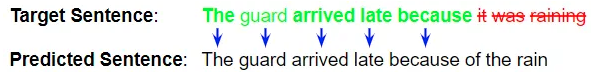
\includegraphics[]{figure/1-gram.png}
    \citebutton{Towards Data Science, Ketan Doshi}{https://towardsdatascience.com/foundations-of-nlp-explained-bleu-score-and-wer-metrics-1a5ba06d812b}
    \label{fig:enter-label}
\end{figure}

Five out of eight 1-grams are correctly predicted:

$\rightarrow p_1 = 5/8$

\vfill
    
\end{vbframe}

% ------------------------------------------------------------------------------

\begin{vbframe}{BLEU score (2)}

\begin{figure}
    \centering
    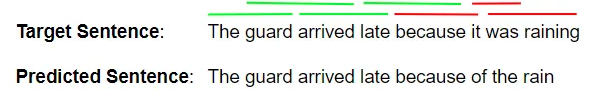
\includegraphics[]{figure/2-gram.png}
    \citebutton{Towards Data Science, Ketan Doshi}{https://towardsdatascience.com/foundations-of-nlp-explained-bleu-score-and-wer-metrics-1a5ba06d812b}
    \label{fig:enter-label}
\end{figure}

Four out of seven 2-grams are correctly predicted:

$\rightarrow p_2 = 4/7$

\textit{You keep doing this procedure until $N$ n-grams and compute a weighted geometric average over the precision scores with weights $w_n$:}

$$exp\left(\sum_{n=1}^{N}w_n\cdot log(p_n)\right)$$
    
\end{vbframe}

% ------------------------------------------------------------------------------

\begin{vbframe}{BLEU Score - Brevity penalty}

\textit{In order to penalize very short predictions (it's more likely for shorter sentences to achieve a good precision score) the BLEU score additionally has a brevity penalty term:}

$$
  BP=\begin{cases}
    1, & \text{if $c>r$}\\
    e^{(1-r/c)}, & \text{if $c\leq r$}
  \end{cases}
$$

\begin{itemize}
    \item With $r$ being the \textbf{reference corpus length} and $c$ the \textbf{candidate corpus length}
    \item The final formula is then:

$$BLEU = BP \cdot exp\left(\sum_{n=1}^{N}w_n\cdot log(p_n)\right)$$
\end{itemize}
    
\end{vbframe}


% ------------------------------------------------------------------------------

\begin{vbframe}{ROUGE score}

\vfill

\begin{itemize}
    \item The ROUGE (Recall-Oriented Understudy for Gisting Evaluation) is a metric commonly used for evaluating the quality of machine-generated text, particularly summaries
    \item ROUGE measures the similarity between the generated summary and one or more reference (human-written) summaries
    \item ROUGE includes multiple metrics, such as ROUGE-N (for n-grams), ROUGE-L (for longest common subsequence), and ROUGE-W (for weighted n-grams). Depending on the task, these metrics capture different aspects of summary quality, allowing a more comprehensive evaluation
\end{itemize}

\vfill
    
\end{vbframe}



% ------------------------------------------------------------------------------

\begin{vbframe}{Example: ROUGE-1 precision}

\vfill
\textit{Consider the following source sentence $S$ and candidate summary $C$:}

\begin{itemize}
    \item \textbf{S:} The cat is on the mat.
    \item \textbf{C:} \textcolor{green}{The cat} and \textcolor{green}{the} dog.
\end{itemize}

\textit{Using the ROUGE-N precision score with $N = 1$ you get:}

\begin{itemize}
    \item Three correctly predicted unigrams
    \item Total of number of unigrams in $C$ is 5
\end{itemize}

$\rightarrow \text{ROUGE-1 precision}=3/5 = 0.6$

\textit{There are more ROUGE scores as mentioned earlier. You can find more details here:} \citebutton{Medium, Fabio Chiusano}{https://medium.com/nlplanet/two-minutes-nlp-learn-the-rouge-metric-by-examples-f179cc285499}
\vfill
    
\end{vbframe}

% ------------------------------------------------------------------------------
\begin{vbframe}{Metrics without a gold reference}

\vfill

\begin{itemize}
    \item BLEU and ROUGE are both used for tasks that have a gold reference you can compare your prediction to
    \item In open ended text generation you just have a prompt and an output generated by the model
    \item You don't have any gold reference to compare your output to
    \item Therefore you have to get a bit more creative with the choice of evaluation metrics
\end{itemize}

\vfill
    
\end{vbframe}

% ------------------------------------------------------------------------------

\begin{vbframe}{Diversity}

\citebutton{Su et al., 2022}{https://arxiv.org/abs/2202.06417} \textit{define diversity in their paper, where they introduce contrastive search, as the generation repetition at different $n$-gram levels}:

\begin{itemize}
    \item \textbf{Generation Repitition:}
    \begin{itemize}
        \item Measures the sequence-level repitition as the portion of duplicate $n$-grams in the generated text
        \item For a generated text continuation $x_{cont}$ the repitition at $n$-gram level is defined as: 
        $$\text{rep-n} = 100 \times \left(1.0 - \frac{|\text{unique $n$-grams}(x_{cont})|}{|\text{total $n$-grams}(x_{cont})|}\right)$$ 
    \end{itemize}
\end{itemize}

\end{vbframe}
% ------------------------------------------------------------------------------

\begin{vbframe}{Diversity (2)}

\vfill

\begin{itemize}
\item \textbf{Diversity:}
    \begin{itemize}
        \item Repitition at different $n$-gram levels:
        $$\text{DIV} = \prod_{n=2}^{4}\left(1.0 - \frac{\text{rep-n}}{100}\right)$$
        \item Plugging in rep-n from the previous slide, this expression simplifies to:
        $$\text{DIV} = \prod_{n=2}^{4} \frac{|\text{unique $n$-grams}(x_{cont})|}{|\text{total $n$-grams}(x_{cont})|}$$
        \item A low diversity score suggests the model suffers from repitition, and a high diversity score means the model-generated text is lexically diverse
    \end{itemize}
\end{itemize}

\vfill
        
\end{vbframe}

% ------------------------------------------------------------------------------

\begin{vbframe}{Coherence}

\textit{This measure was also proposed by \citebutton{Su et al., 2022}{https://arxiv.org/abs/2202.06417} as the cosine similarity between the sentence embeddings of the prompt $x_{prompt}$ and a generated text conitinuation $x_{cont}$}:

\begin{itemize}
    \item They use pre-trained SimCSE sentence embeddings $EMB(x)$ proposed by \citebutton{Gao et al., 2022}{https://arxiv.org/abs/2104.08821}:
    $$COH(x_{cont}, x_{prompt}) = \frac{EMB(x_{prompt}) \cdot EMB(x_{cont})}{\Vert EMB(x_{prompt})\Vert \cdot \Vert EMB(x_{cont})\Vert}$$
    \item The higher the coherence-score the better the model-generated text fits to the given prompt
\end{itemize}
    
\end{vbframe}

% ------------------------------------------------------------------------------

\begin{vbframe}{MAUVE}
\citebutton{Pillutla et al., 2021}{https://arxiv.org/abs/2102.01454}

\vfill

\begin{itemize}
    \item A language model is an estimate $\hat{P}(x)$ of the probability distribution over sequences of text $x = (x_1, . . ., x_{|\mathbf{x}|})$, consisting of tokens $x_t$ belonging to a fixed vocabulary
    \item Given a context $x_{1:t}$, a language model $\hat{P}$ and a stochastic decoding strategy we generate text by sampling $\hat{x}_{t+1} \sim \hat{P}(\cdot|x_{1:t}), \hat{x}_{t+2} \sim \hat{P}(\cdot|x_{1:t}, \hat{x}_{t+1})$, etc.
    \item The decoding strategy and the language model taken together define a distribution $Q$ over text, which we call \textit{model distribution}
    \item The goal of MAUVE is to measure the gap between the model distribution $Q$ and the target distribution $P$
\end{itemize}

\vfill
    
\end{vbframe}

% ------------------------------------------------------------------------------

\begin{vbframe}{Sources of error in text generation}

\begin{figure}
    \centering
    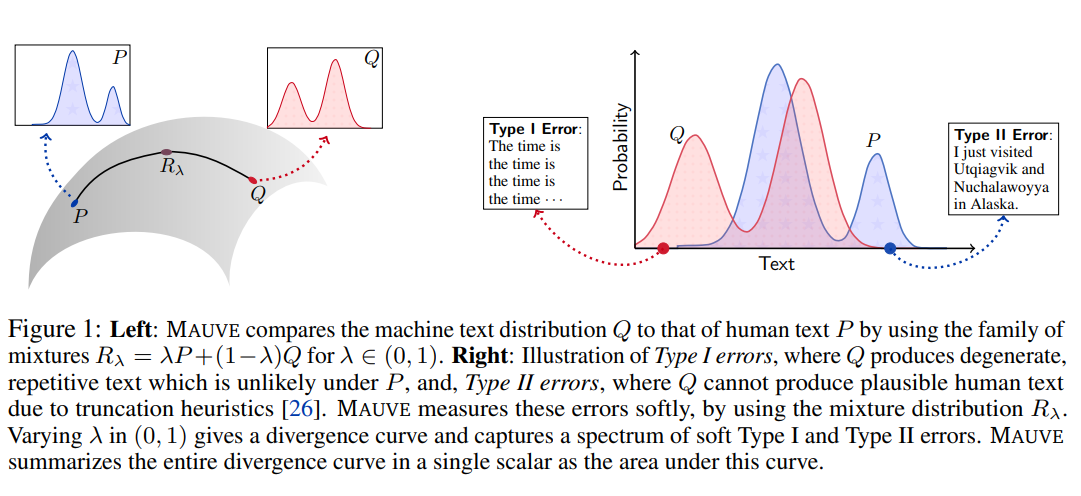
\includegraphics[]{figure/mauve_errors.png}
\end{figure}

\begin{itemize}
    \item The gap between $Q$ and $P$ arises from two sources of error
    \item Type I error: $Q$ places high mass on text which is unlikely under $P$
    \item Type II error: $Q$ cannot generate text which is plausible under $P$
\end{itemize}

\begin{itemize}
    \item They formalize the two errors through the Kullback-Leibler divergence:
        \begin{itemize}
            \item $KL(Q|P)$ penalizes $Q$ if there is a text $x$ that leads to a high $Q(x)$ but a low $P(x)$, which is the Type I error
            \item Similarly the Type II error is defined by $KL(P|Q)$
        \end{itemize}
    \item Issue: both KL divergences are infinite if the supports of $Q$ and $P$ are not identical
    \item The authors overcome this issue by \textit{softly} measuring the two errors with a mixture distribution: 
    $$R_{\lambda} = \lambda P (1-\lambda) Q \quad \text{for} \quad \lambda \in (0,1)$$
    \item (soft) Type I error: $KL(Q,R_{\lambda})$
    \item (soft) Type II error: $KL(P,R_{\lambda})$
\end{itemize}

\end{vbframe}

% ------------------------------------------------------------------------------

\begin{vbframe}{Divergence Curve}

\begin{figure}
    \centering
    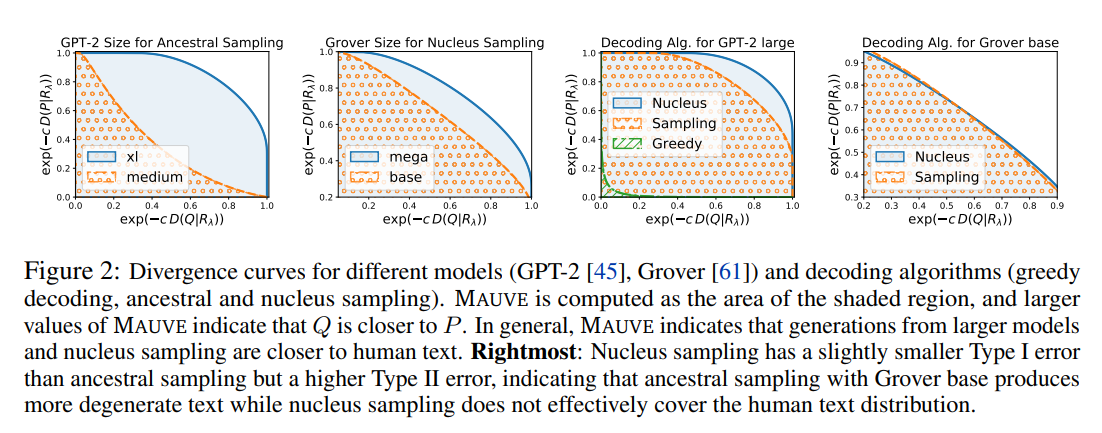
\includegraphics[]{figure/mauve_divergence.png}
\end{figure}

\begin{itemize}
    \item To capture all the possible values of the mixture weight $\lambda$ they vary $\lambda$ between 0 and 1 to generate a \textit{divergence curve}:
\end{itemize}
\scalebox{0.85}{% 
$C(P,Q) = \left\{(exp(-cKL(Q|R_{\lambda})), exp(-cKL(P|R_{\lambda})) : R_{\lambda} = \lambda P + (1-\lambda) Q, \lambda \in (0,1)\right\}$}
\begin{itemize}
    \item $MAUVE(P,Q)$ is the area under this divergence curve, it is a summary of the trade-off between Type I and II errors and lies in (0,1] (more details can be found in the paper \citebutton{Pillutla et al., 2021}{https://arxiv.org/abs/2102.01454})
\end{itemize}
    
\end{vbframe}
% ------------------------------------------------------------------------------

\begin{vbframe}{Human evaluation}

\textbf{Why Human Evaluation?}
\begin{itemize}
    \item \textbf{Subjectivity of Quality}: Human judgments are essential for evaluating the nuanced quality of text that automatic metrics might miss, such as humor, creativity, and relevance
\end{itemize}

\textbf{Key Considerations}
\begin{itemize}
    \item \textbf{Evaluators}: Use domain experts or crowdworkers, depending on the task complexity
    \item \textbf{Evaluation Criteria}:
    \begin{itemize}
        \item \textbf{Fluency}: Is the generated text grammatically correct and natural-sounding?
        \item \textbf{Coherence}: Does the text make logical sense?
        \item \textbf{Diversity}: Is the output lexically diverse?
    \end{itemize}
    \item \textbf{Challenges}: 
    \begin{itemize}
        \item \textbf{Subjectivity}: Different evaluators might have varying opinions, leading to inconsistency
        \item \textbf{Cost and Time}: Human evaluation is resource-intensive
        \item \textbf{Bias}: Evaluators might bring in their biases, which can skew results
    \end{itemize}
\end{itemize}
   
\end{vbframe}

% ------------------------------------------------------------------------------


%%%%%%%%%%%%%%%%%%%%%%%%%%%%%%%%%%%%%%%%%%%%%%%%%%%%%%%%%%%%%%%%%%
\section{Fine-Tuning and Prompting}
% Source: DL4NLP chapter09-llm/slides-91-instruction-tuning.tex
%%%%%%%%%%%%%%%%%%%%%%%%%%%%%%%%%%%%%%%%%%%%%%%%%%%%%%%%%%%%%%%%%%
%\lecturechapter{Fine-Tuning}
%\begin{frame}{REINSTATE LECTURE COMMAND}
%\end{frame}

%\lecture{Deep Learning for NLP}

% ------------------------------------------------------------------------------

\begin{frame}{recap}

\vfill

\begin{itemize}
    \item language modeling objective
        \begin{itemize}
            \item masking and next token prediction
            \item no explicit understanding of tasks
        \end{itemize}
    \item this is true for encoder and decoder models
    \item So we need to do additional work if we want
        to use language models for solving tasks!
\end{itemize}

\vfill

\end{frame}


\begin{frame}{How to solve a task with language models? (1)}

\vfill

\begin{itemize}
    \item ``old-style'' single-task fine-tuning 
        \begin{itemize}
            \item supervised training
of the pretrained model
on a task-specific
        training set of size $k$ (where $k$ is not small,
        e.g., $k=100$)
        \end{itemize}
\end{itemize}

\vfill

\end{frame}

\begin{frame}{BERT finetuning example 1}

\vfill
	
	\begin{figure}
		\centering
		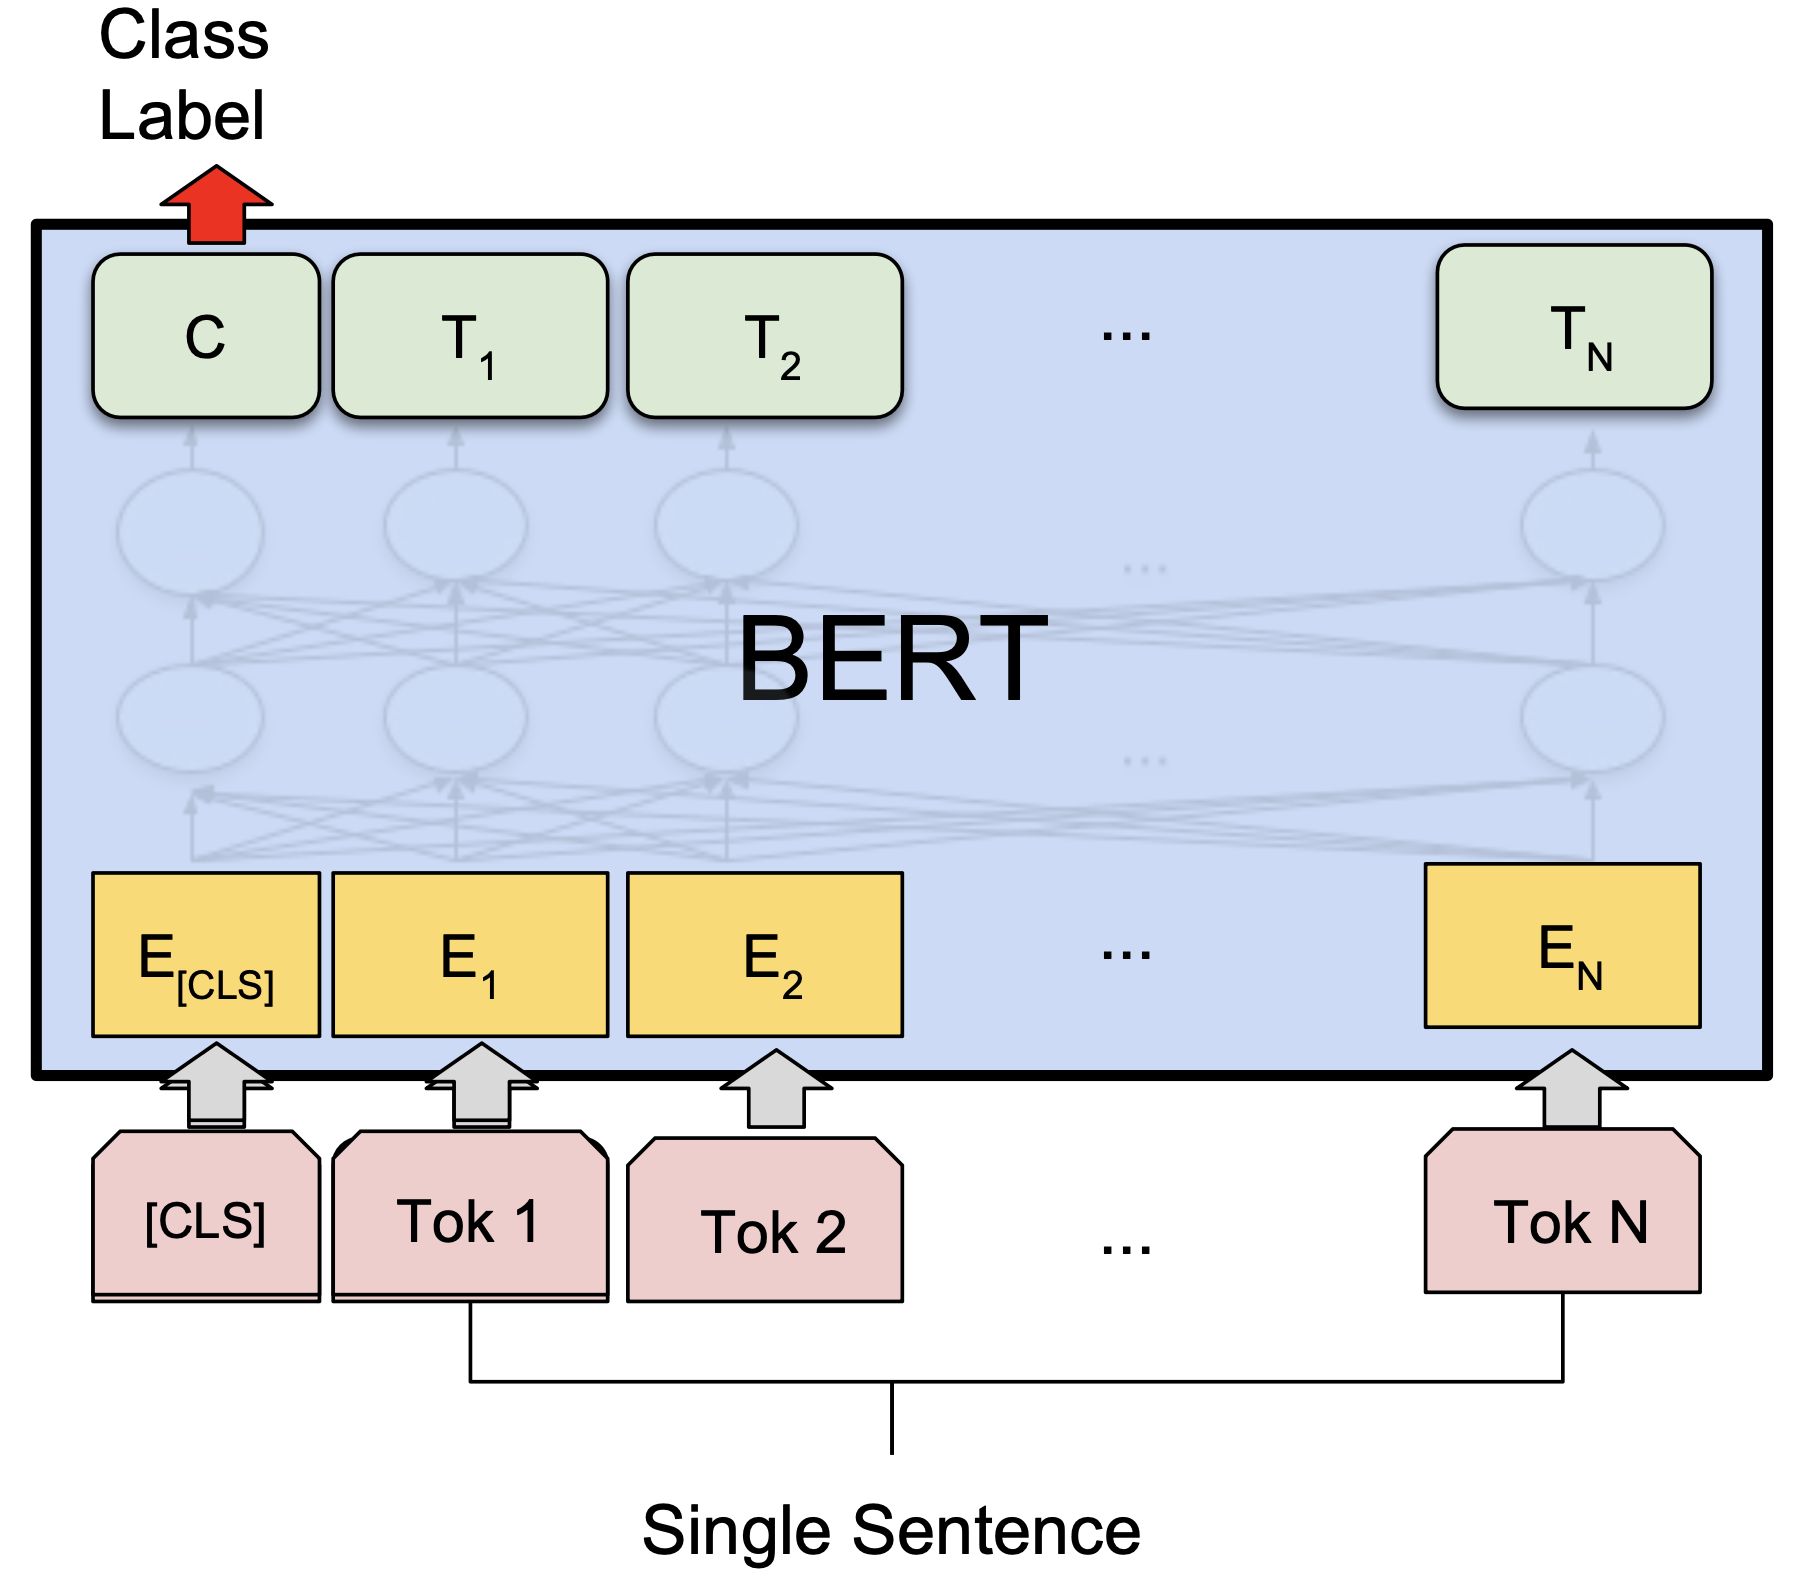
\includegraphics[height = 6cm]{figure/bertfinetune1} 
	\end{figure}

\vfill

\end{frame}
\begin{frame}{BERT finetuning example 2}

\vfill
	
	\begin{figure}
		\centering
		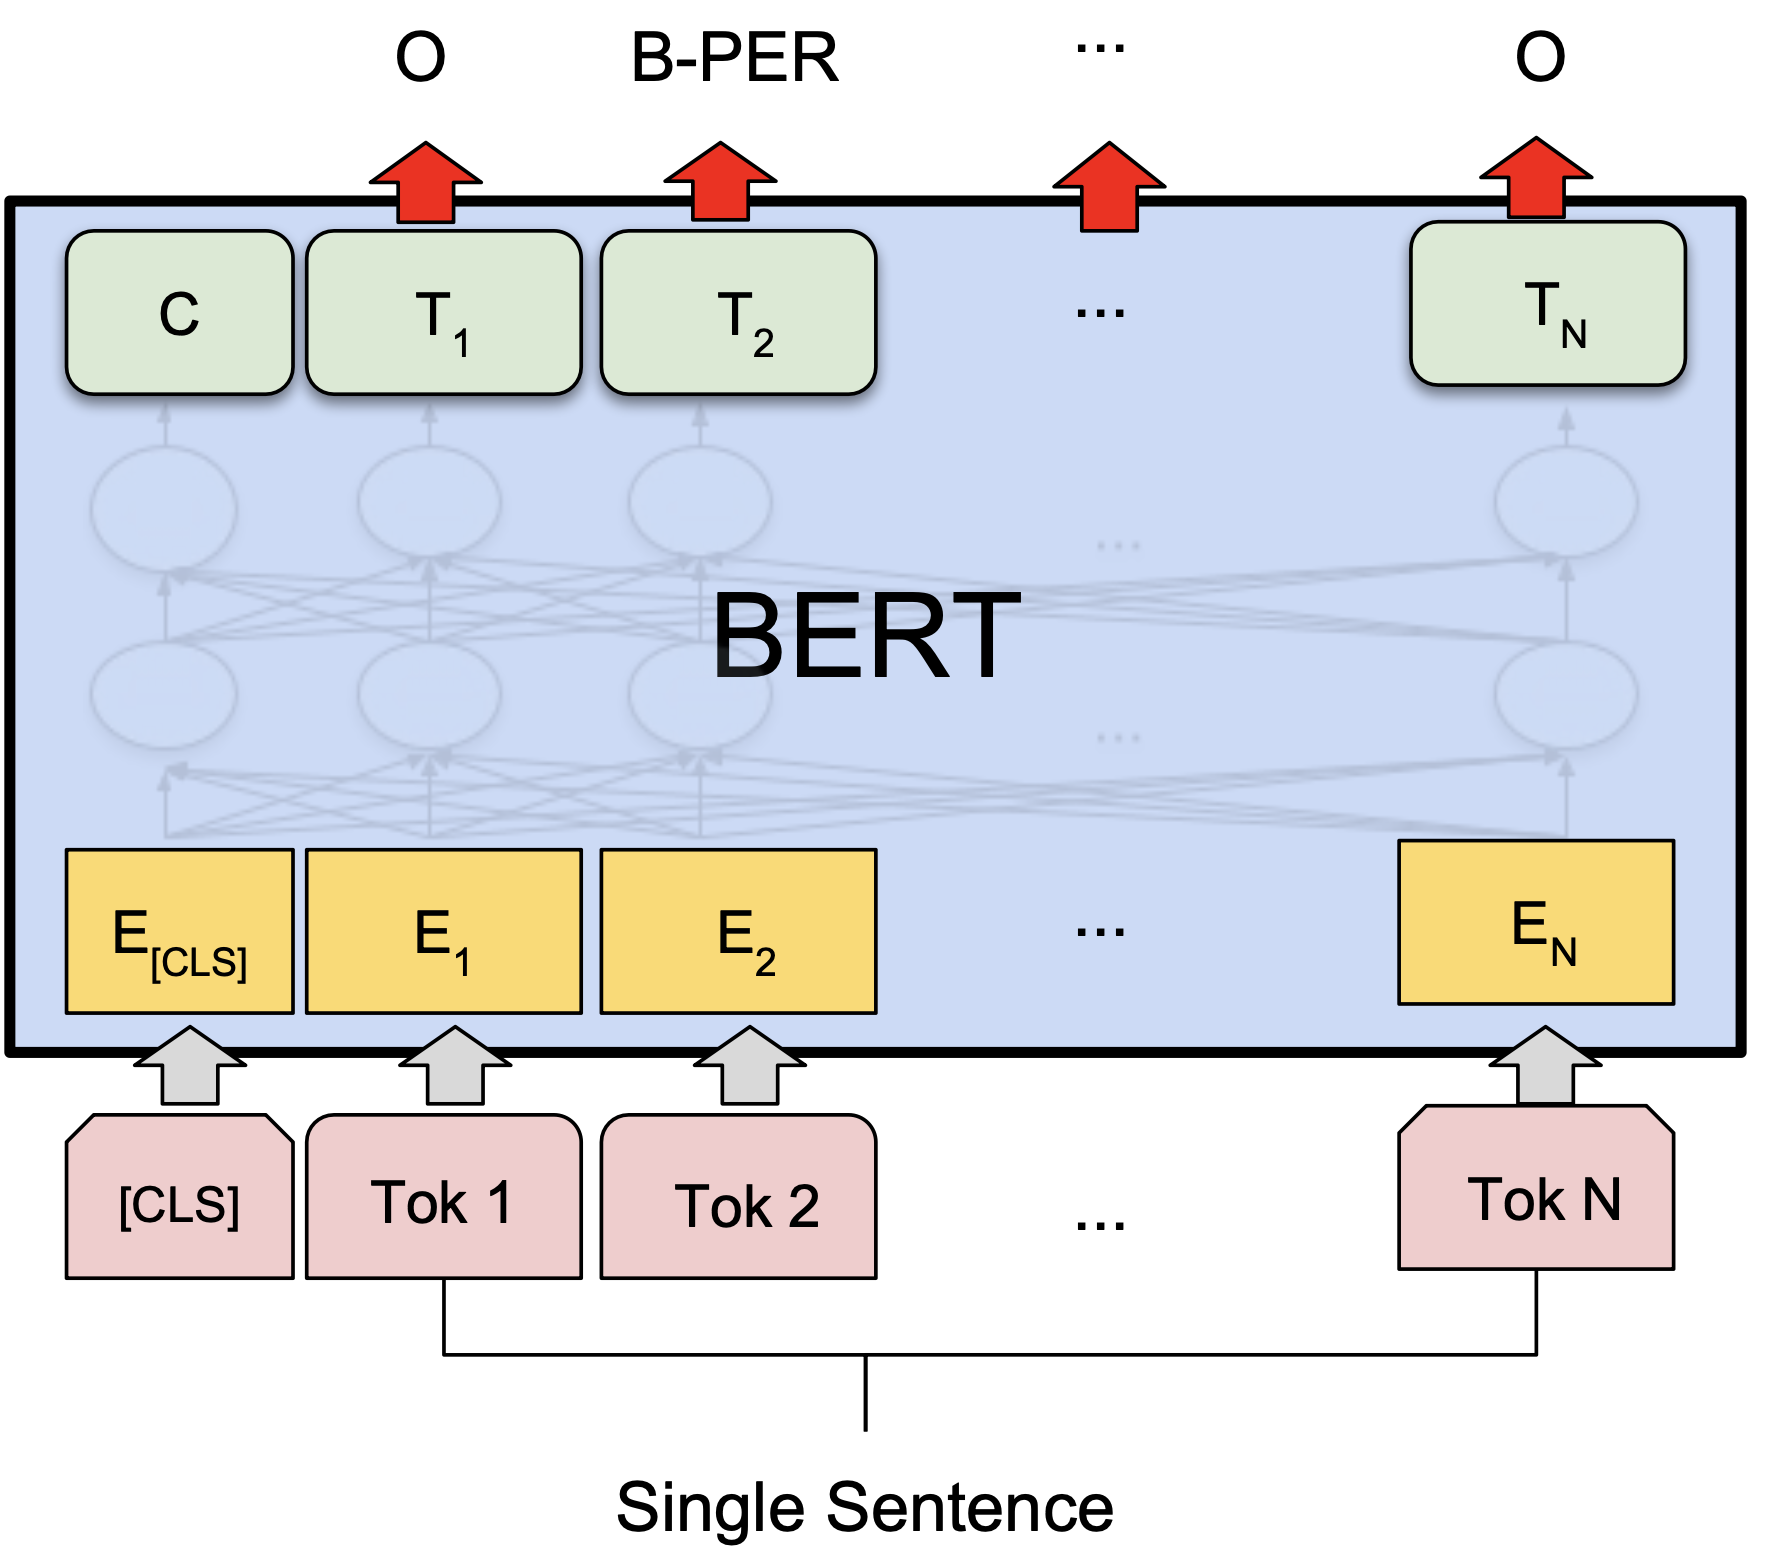
\includegraphics[height = 6cm]{figure/bertfinetune2} 
	\end{figure}

\vfill

\end{frame}


\begin{frame}{How to solve a task with language models? (1)}

\vfill

\begin{itemize}
    \item ``old-style'' single-task fine-tuning 
        \begin{itemize}
            \item supervised training
of the pretrained model
on a task-specific
        training set of size $k$ (where $k$ is not small,
        e.g., $k=100$)
        \item the output can be an arbitrary category (e.g.,
        ``0'', ``1'' for sentiment analysis)
        \item (this is the typical way encoder models like
        BERT are used)
            \item alternatively, the output can be a
        meaningful ``verbalizer'' (e.g., ``negative'',
        ``positive'' for sentiment analysis)
        		\citebutton{Schick et al.,
        2020}{https://arxiv.org/abs/2009.07118}
        \item still very much relevant if you need to deploy
        a small efficient model for a focused task
        \end{itemize}
\end{itemize}

\vfill

\end{frame}




\begin{frame}{Verbalizer}

\vfill
	
	\begin{figure}
		\centering
		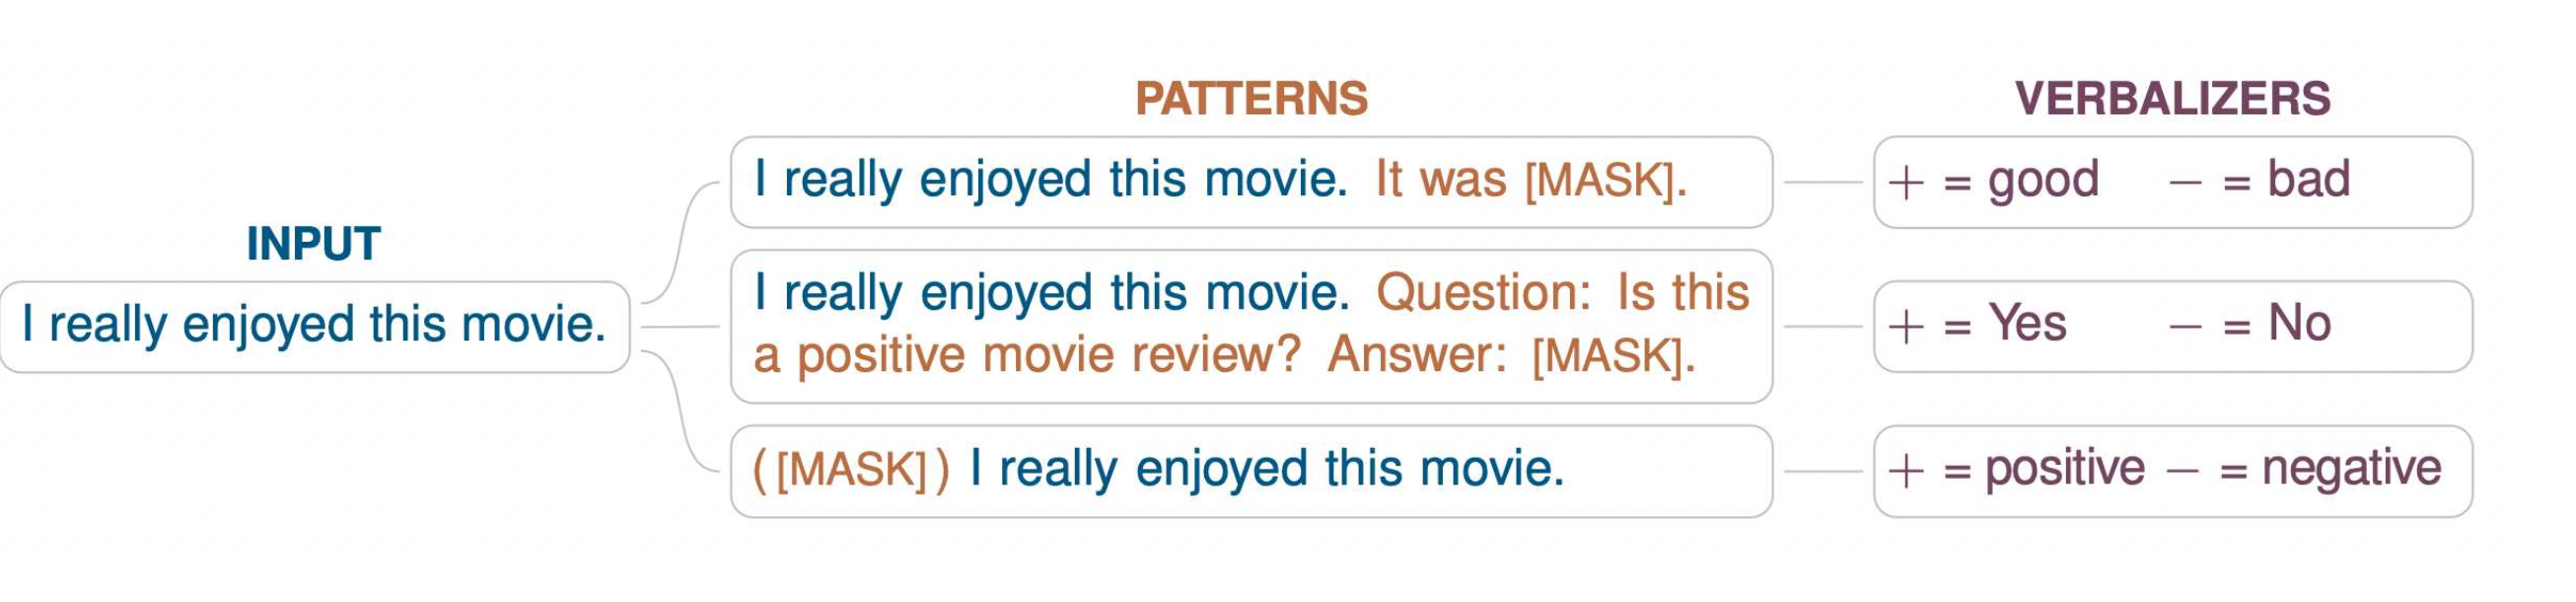
\includegraphics[width = 12cm]{figure/schickverbalizer} 
	\end{figure}

\vfill

\end{frame}




\begin{frame}{Verbalization: Summary}

\vfill

\begin{itemize}
    \item Finetuning a language model on predicting
      meaningful labels (``good'', ``bad'') requires less
      data than finetuning on classical NLP labels like ``0'' and ``1''.
\item Reason: The language model understands the labels
  already, so it doesn't have to learn them.
        \end{itemize}


\vfill

\end{frame}




\begin{frame}{How to solve a task with language models? (2)}

\vfill

\begin{itemize}
    \item few-shot prompting
        \begin{itemize}
            \item provide, in-context,  $k$ (where $k$ is small, e.g., $k=5$) examples of what the model is
supposed to do
        \item the model will then often complete the task
        just based on analogy to these few shots
        \item this is a typical way of using current
        autoregressive models for tasks
\item no change to the parameters of the model, i.e., no training
\end{itemize}
\end{itemize}

\vfill

\end{frame}

\begin{frame}{few-shot prompting example}

\vfill
	
	\begin{figure}
		\centering
		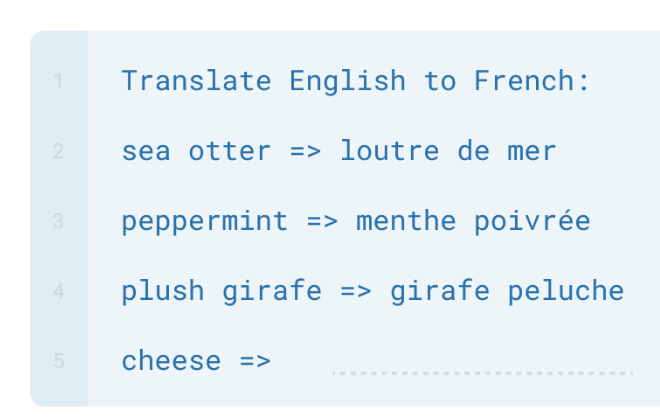
\includegraphics[height = 5.10cm]{figure/fewshotprompting} 
	\end{figure}

(from gpt3 paper -- ``Translate English to French'' should
appear four times to make it a 3-shot example that has 3
identical shots as required by the definition of few-shot prompting)

\vfill

\end{frame}


\begin{frame}{How to solve a task with language models? (3)}

\vfill

\begin{itemize}
\item multi-task finetuning
        \begin{itemize}
        \item finetuning on a large training set of *many* tasks
        \item the more tasks the better
        \item method 1: consistent task format, e.g., each
        task is reformulated into a question-answering format
        \item method 2: more open task format
\item ideally: task format includes ``instructions'',
similar to verbalizer
            \item Examples: T0, T5 and FLAN, see below
        \end{itemize}
\end{itemize}

\vfill

\end{frame}

\devour{

\begin{frame}{How do solve a task with language models? (4)}

\vfill

\begin{itemize}
\item instruction tuning (short for instruction finetuning)
        \begin{itemize}
            \item you teach the model a *general*
            capability of being ``helpful''
            \item it then solves arbitrary tasks without few-shot
            prompting and without additional finetuning
            \item theory/hope: you no longer have to explicitly
            train on specific tasks, the instruction-tuned
            model can solve new tasks without having been
            trained on them
            \item next lecture
        \end{itemize}
\end{itemize}

\vfill

\end{frame}
}

% ------------------------------------------------------------------------------

% ------------------------------------------------------------------------------

\begin{frame}{Other types of finetuning (1)}

\vfill

\begin{itemize}
    \item Finetuning has yet another meaning.
    \item Continued pretraining is also sometimes called
    finetuning.
    \item Continued pretraining: given a language model
that has been    trained on generic data (web, reddit etc),
    adapt it to a new domain (e.g., company-internal data) by
    training it on a large corpus from this new domain.
\item objective: standard language modeling objective
    \item This results in a language model that has all the
    nice capabilities of a generic language model, but also understands the special domain.
\item Not trivial to do well
\end{itemize}

\vfill

\end{frame}



\begin{frame}{Continued pretraining}

\vfill
	
	\begin{figure}
		\centering
		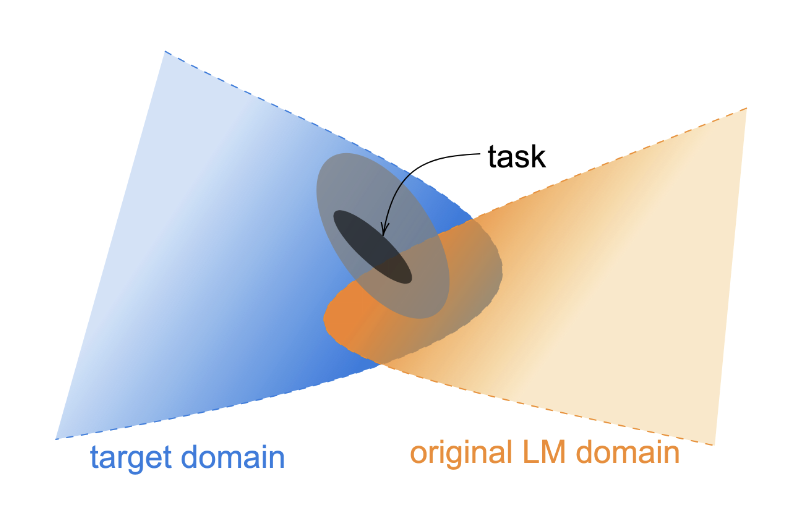
\includegraphics[height = 6cm]{figure/continuedpretraining1} 
	\end{figure}

\vfill

\end{frame}

  \devour{

    \begin{frame}{Continued pretraining}

\vfill
	
	\begin{figure}
		\centering
		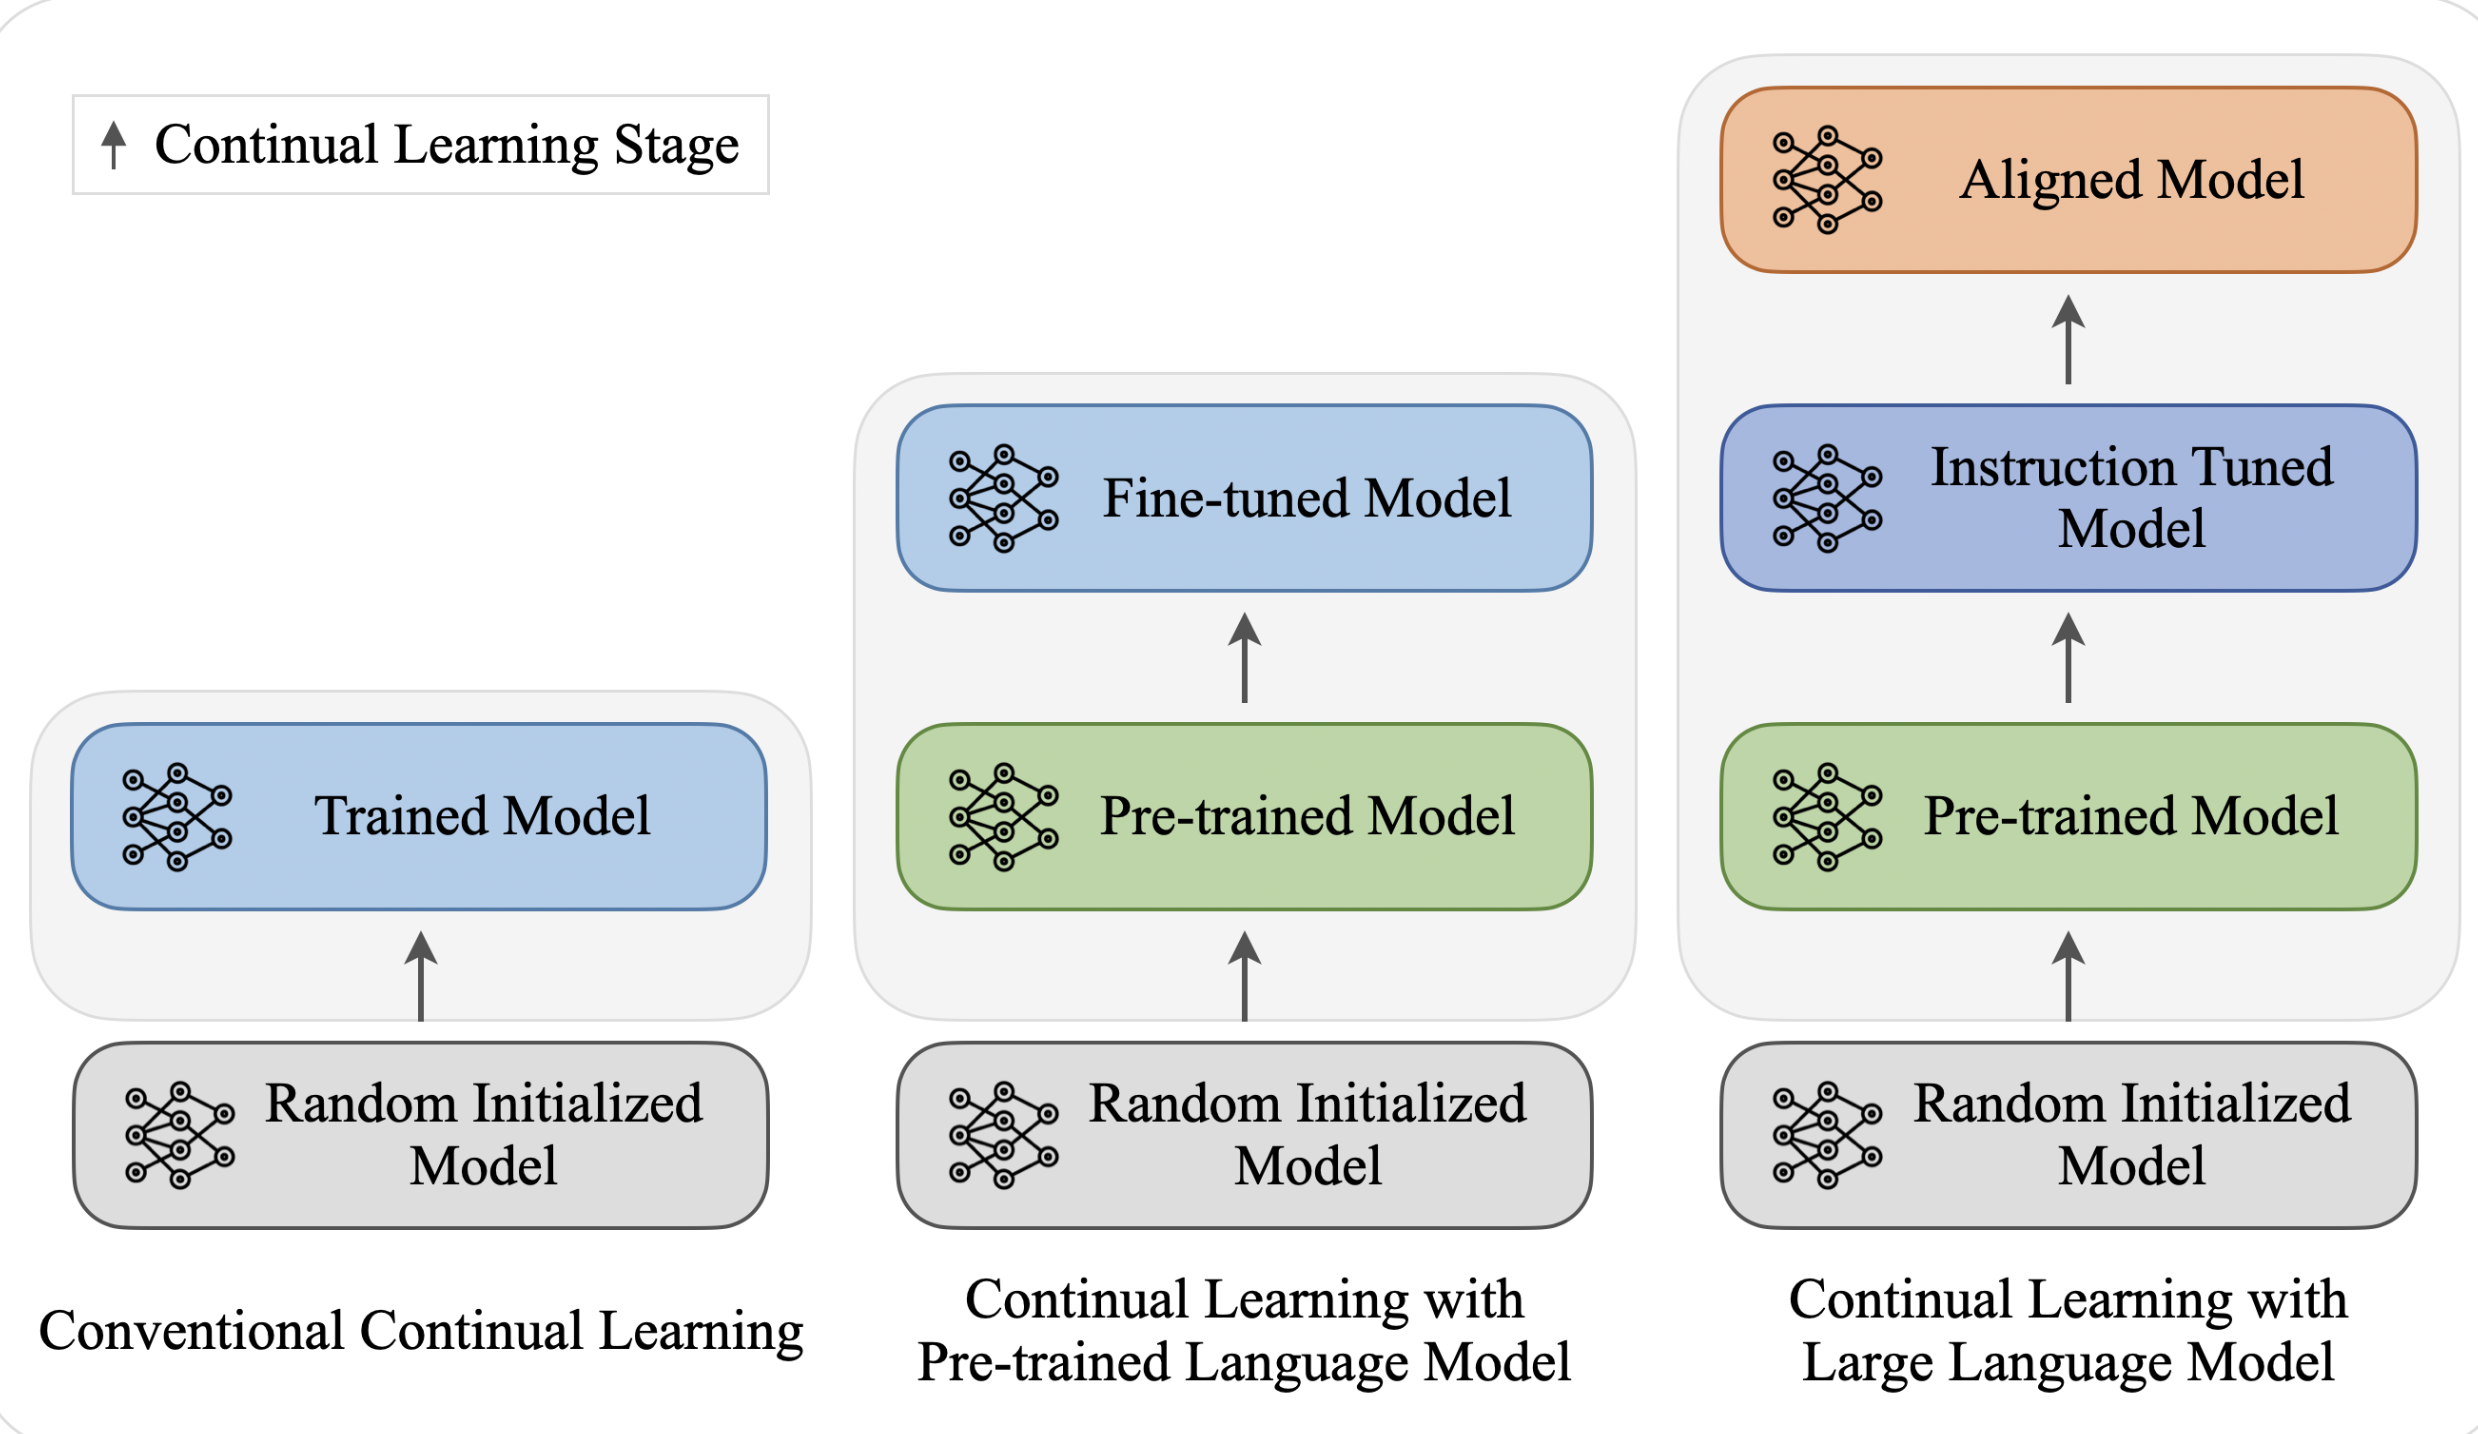
\includegraphics[height = 6cm]{figure/continuedpretraining2} 
	\end{figure}

\vfill

\end{frame}


}


\begin{frame}{Terminology}

\vfill

\begin{itemize}
  \item This lecture
\begin{itemize}
\item single-task finetuning
\item multi-task finetuning
\item prompting\\
(this is definitely not finetuning)
\item continued pretraining
\item \ques terminology clear?
\end{itemize}
\item Next lecture
  \begin{itemize}
\item instruction tuning\\ (can be seen as a form of finetuning)
\item reinforcement learning\\
  (can also be done through a form of finetuning)
\end{itemize}
\end{itemize}

\vfill

\end{frame}


% ------------------------------------------------------------------------------


% ------------------------------------------------------------------------------

%\begin{frame}{pre-trained generative models}
%
%\vfill
%	
%	\begin{figure}
%		\centering
%		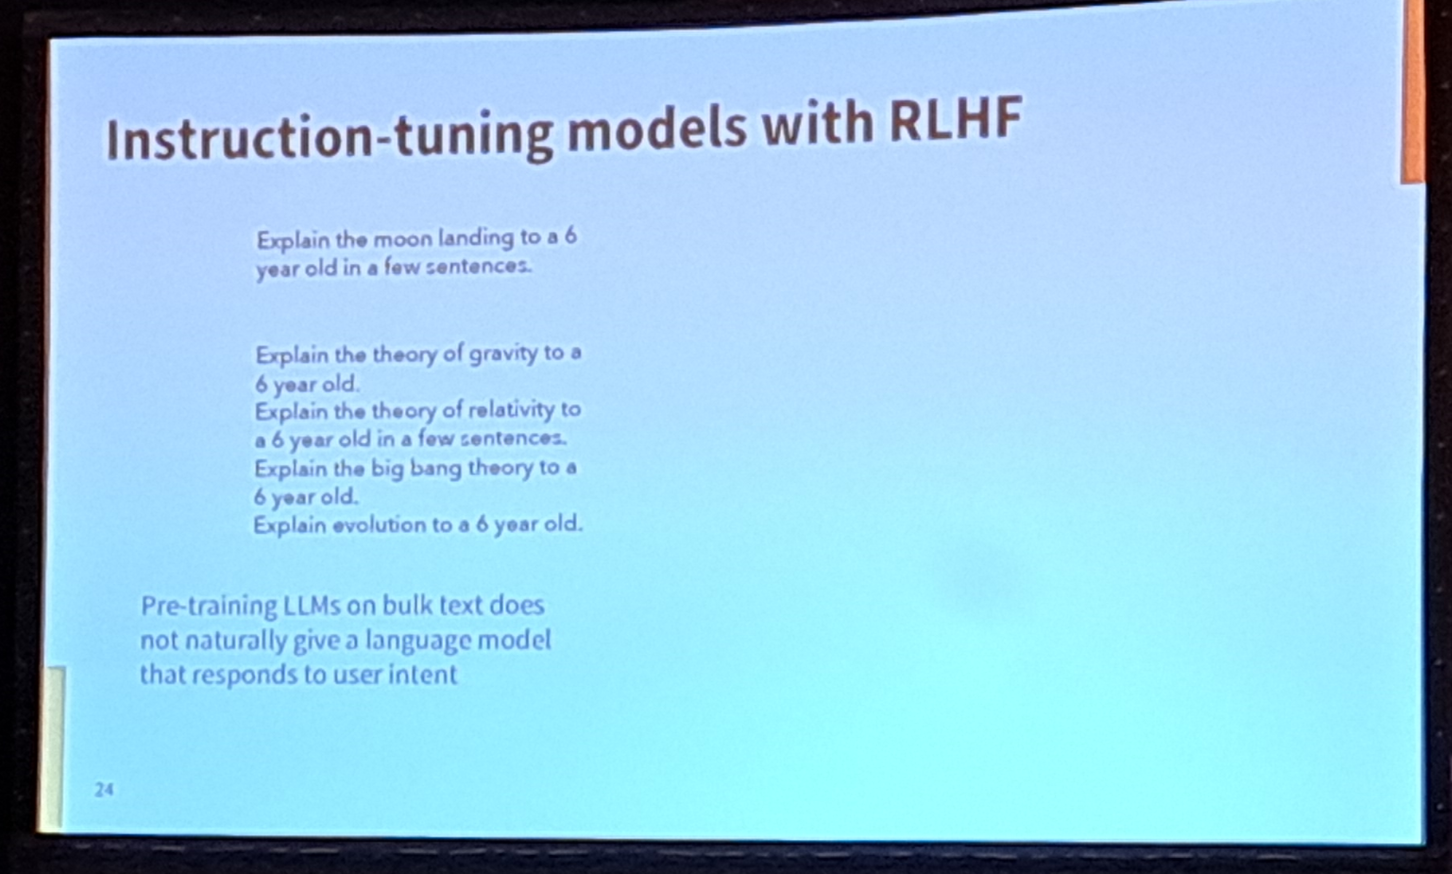
\includegraphics[width = 11cm]{figure/manning.png}\\ 
%		Source: Chris Manning's keynote at EMNLP 2023
%	\end{figure}
%
%\vfill
%
%\end{frame}

% ------------------------------------------------------------------------------

%\begin{frame}{agenda}
%
%\vfill
%
%\begin{itemize}
%    \item \textit{chain-of-thought prompting:}
%        \begin{itemize}
%            \item trigger the model to ''explain'' it thought-process
%            \item final goal still correct label/output
%        \end{itemize}
%    \item \textit{emergent abilities:}
%        \begin{itemize}
%%%%%%%%            \item \textit{claim:} With increasing model sizes, at some point new capabilities of the models (seem to) ''emerge''.
%        \end{itemize}
%\end{itemize}
%
%\vfill
%
%\end{frame}

% ------------------------------------------------------------------------------

\begin{frame}{issues with single-task fine-tuning}

\vfill

\begin{itemize}
    \item The result is a single-task model.
%\item Sequential transfer learning instead of true multi-task learning
\begin{itemize}
    \item Generalization of the model 
             is only w.r.t. to one task / data distribution
\end{itemize}
    \item Requires  annotated
        data (e.g., $k=100$)
%    \item Single-task models have poor few-shot capabilities
            \item \ques Could there be other tasks that
        might benefit?
 %           \item \ques What about related domains / languages?
\end{itemize}

\vfill

\end{frame}



% ------------------------------------------------------------------------------
\begin{frame}{issues with few-shot prompting: (1) classification}

\vfill

\begin{itemize}
    \item Assumption: Model has learned about the task during (unsupervised) pre-training 
    \item Write prompt so that  a direct response must be
    given by the language model.
\begin{itemize}
        \item Just a label, just yes/no answer, just a name
    in QA
\end{itemize}
    \item This is not natural dialogic behavior: humans
    typically don't
    just answer with a label, yes/no, a name (although
    sometimes they do)
    \item See next lecture
%\item Again: Prompting works best if the task has occurred during
%unsupervised training.
\item Current use of the word ``prompt'' is more general: basically
anything you type into the LLM context window
 %   \item \ques For which tasks is this expected to work well?
% key: does the task (or as imilar task) occur in preatraing
% machine translation example:  example of what works well
% complex reasoning example: example of what does notw ork well
%    \item \textit{Lack of interpretability}
%    \begin{itemize}
%        \item Just the answer w/o explanation
%        \item Big concern about LLMs in general

%    \item \textit{Misalignment with human needs}
%    \begin{itemize}
%        \item Out of context answers
%        \item Harmful answers
%    \end{itemize}
\end{itemize}

\vfill

\end{frame}


\begin{frame}{issues with few-shot prompting:\\ (2) text generation}

\vfill

\begin{itemize}
%\item Very similar to (1) classification
    \item Again, assumption: Model has learned about the task during (unsupervised) pre-training 
    \item Again: Write prompt so that  a direct response must be
    given by the language model.
\item Works best if the task has occurred during
unsupervised training.
    \item \ques For which tasks is this expected to work well?
% summarization, translation because they occur in
% pretraining data
\end{itemize}

\vfill

\end{frame}



% ------------------------------------------------------------------------------

%\begin{frame}{issues with prompting}
%
%\vfill
%
%\begin{itemize}
%    \item \textit{Hallucinations:} Output that is not true.
%(different possible causes: just made up,
%incorrect internal reasoning etc)
%    \item \textit{Imprecise mathematical operations:} Models not trained to do arithmetics
%    \item \textit{Inadequate experience grounding:} Not
%    fully capable of generating correct answers to questions
%    from specialized domains not covered by pretraining data
%    \item \textit{Limited ability for complex reasoning:} Long-known challenge in NLP/LLMs
%\end{itemize}
%
%\vfill
%
%\end{frame}
%
%% ------------------------------------------------------------------------------

%\begin{frame}{issues with prompting}
%
%\vfill
%
%\begin{itemize}
%% if you believe that you can find everything on the web: yes
%% however: see point "grounding in specialized domain" in a few slides
%    \end{itemize}
%
%
%\vfill
%
%\end{frame}


\begin{frame}{Multi-task learning: FLAN/T0/T5}

\vfill
	
	\begin{figure}
		\centering
		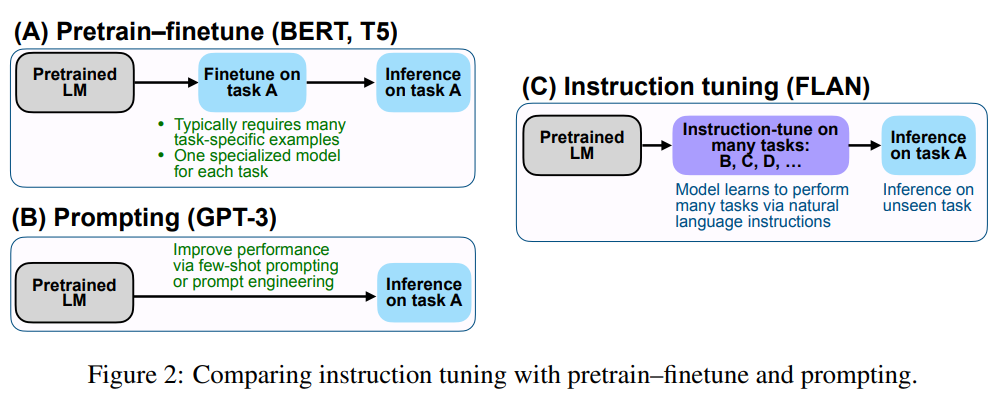
\includegraphics[width = 11cm]{figure/81-flan.png}\\ 
		\citebutton{Source: Wei et al., 2021}{https://arxiv.org/abs/2109.01652}
	\end{figure}

\vfill

\end{frame}


\begin{frame}{Initial Approach:\\
    Multitask finetuning: best of both worlds
(finetuning and  prompting)}

\vfill
	
	\begin{figure}
		\centering
		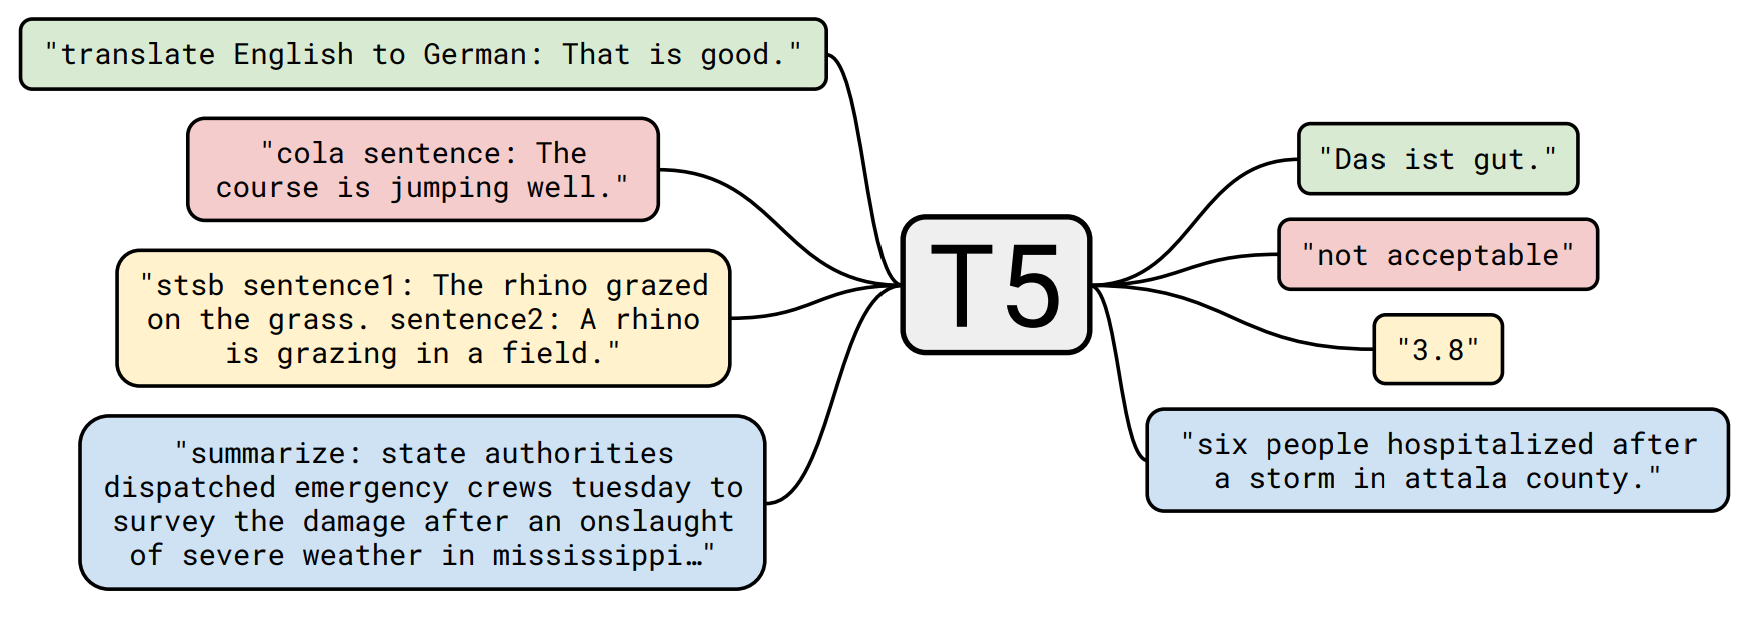
\includegraphics[width = 9.35cm]{figure/62-t5.png}\\ 
		\citebutton{Source: Raffel et al., 2020}{https://jmlr.org/papers/v21/20-074.html}
	\end{figure}

\pause

     \ques What exactly does the model learn here? How well
    would we expect this to generalize to new tasks?
    % IMPLICITLY, i.e. the model learns via fine-tuning which task prefix to associate with which set of labels
% how similar is the new task to an old task
% how good is the formulation to the new task
% does the new task occur in training data
% is the prompt self-explanatory? e.g., it is not for "cola sentence"


\vfill

\end{frame}

% ------------------------------------------------------------------------------

\devour{
\begin{frame}{Construction of training set}

\vfill
	
	\begin{figure}
		\centering
		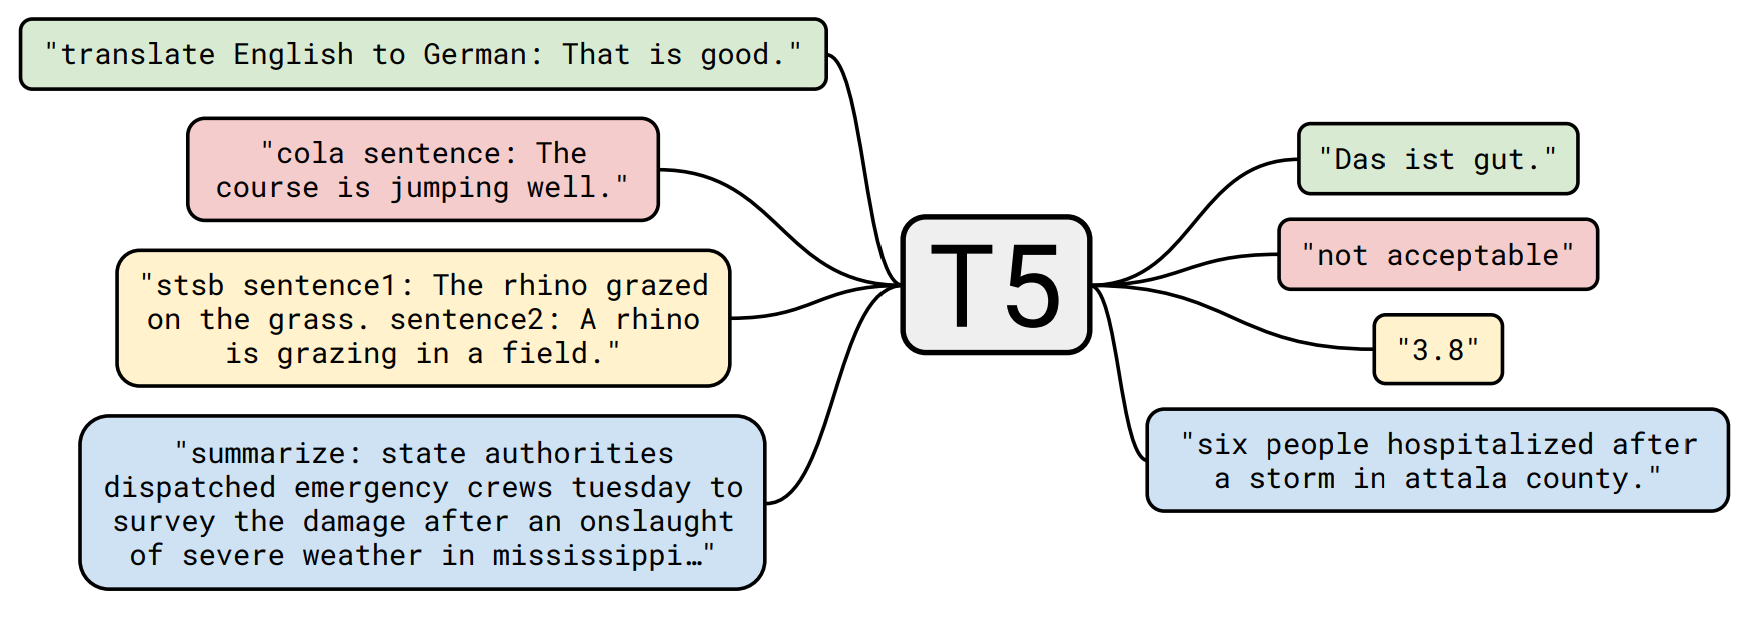
\includegraphics[width = 8cm]{figure/62-t5.png}\\ 
		\citebutton{Source: Raffel et al., 2020}{https://jmlr.org/papers/v21/20-074.html}
	\end{figure}

\pause

\begin{itemize}
    \item \ques The format used here is not just any
    format, but it has a special property. Which property is this?

%\item A consistent format (as in T5) is desirable.


%How can we make the \textit{EXPLICIT}?
%    \item[$\to$] Mapping any natural language tasks into
%    a \textit{human-readable} prompted form
%\citebutton{Schick et al.,
%        2020}{https://arxiv.org/abs/2009.07118},
%\citebutton{Sanh et al., 2021}{https://arxiv.org/abs/2110.08207}
\end{itemize}

\vfill

\end{frame}




% ------------------------------------------------------------------------------

\begin{frame}{Carefully designing task formats (mostly prefixes)}

\vfill
	
	\begin{figure}
		\centering
		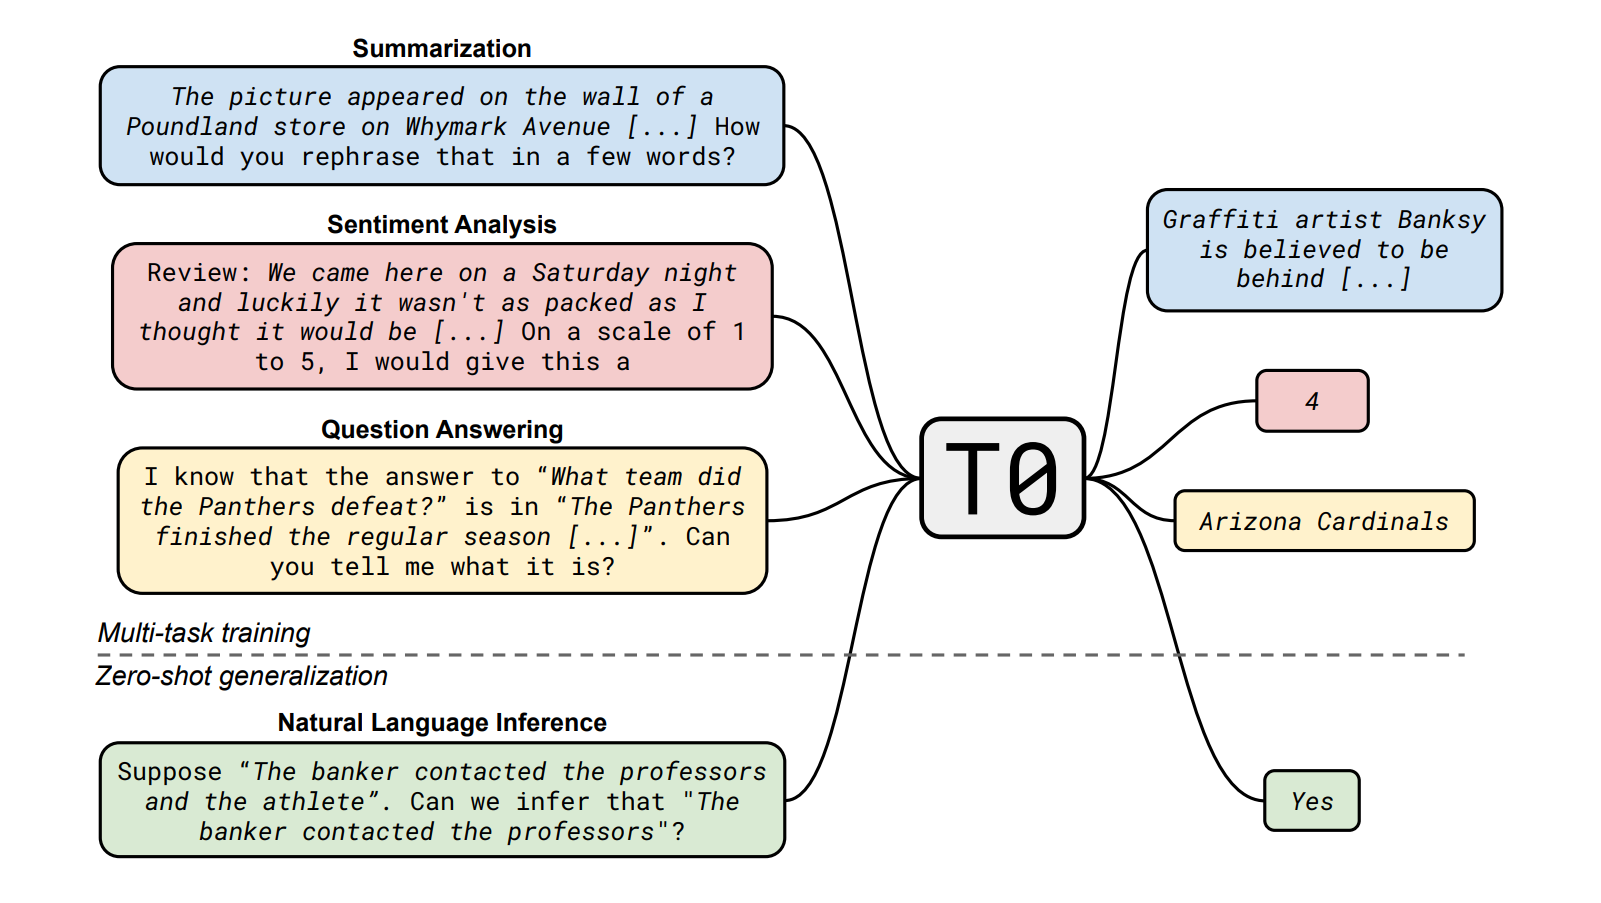
\includegraphics[width = 11cm]{figure/81-t0.png}\\ 
		\citebutton{Source: Sanh et al., 2021}{https://arxiv.org/abs/2110.08207}
	\end{figure}

\vfill

\end{frame}
}
% ------------------------------------------------------------------------------

\begin{frame}{Multitask Prompted
		Training}

\vfill

\begin{itemize}
    \item Multitask Prompted Training
    involves learning from multiple
    tasks using \textbf{unified prompt formats} as a means to improve
    generalization to new, unseen tasks.
    \item (as opposed to T5: non-unified)
    \item This means that the model can perform well on tasks it hasn't been explicitly trained on.
    \item The key for this lies in the set of shared prompts it has learned from during fine-tuning.
\end{itemize}

\vfill

\end{frame}

% ------------------------------------------------------------------------------

\begin{frame}{Multitask Prompted Training}

\vfill

\begin{itemize}
    \item Benchmark for Evaluation:
        \begin{itemize}
        \item Instead of using held-out *samples* (as is
        standard in NLP) \ldots
        \item \ldots we now use held-out *tasks*
%            \item Held-out \textit{tasks} instead of just held-out samples as a test set\\
            \item All data sets belonging to a held-out task go to the test set
            \item Generalization across tasks %/ data distributions
        \end{itemize}
    \item The ``prompts'' are key here to
facilitate
        transfer to new tasks:  the model can solve new
        tasks by generalizing from  the train prompts and the ability to generate text outputs.
\end{itemize}

\vfill

\end{frame}

% ------------------------------------------------------------------------------


\begin{frame}{Typical NLP task:\\ Coreference resolution}

\vfill

\begin{itemize}
    \item One of the tasks on the next slide
    \item In the simplest case the task is to determine
    which noun phrase a referring expression like ``she'' or
    ``this person'' is referring to.
    \item Example: ``Peter helped Paul because he was
      familiar with the problem.''
      \item What does ``he'' refer to?
%    \item ``he'' refers to Peter, not to Paul.
    \end{itemize}

\vfill

\end{frame}

% ------------------------------------------------------------------------------

\begin{frame}{T0: training and test tasks}

\vfill
	
	\begin{figure}
		\centering
		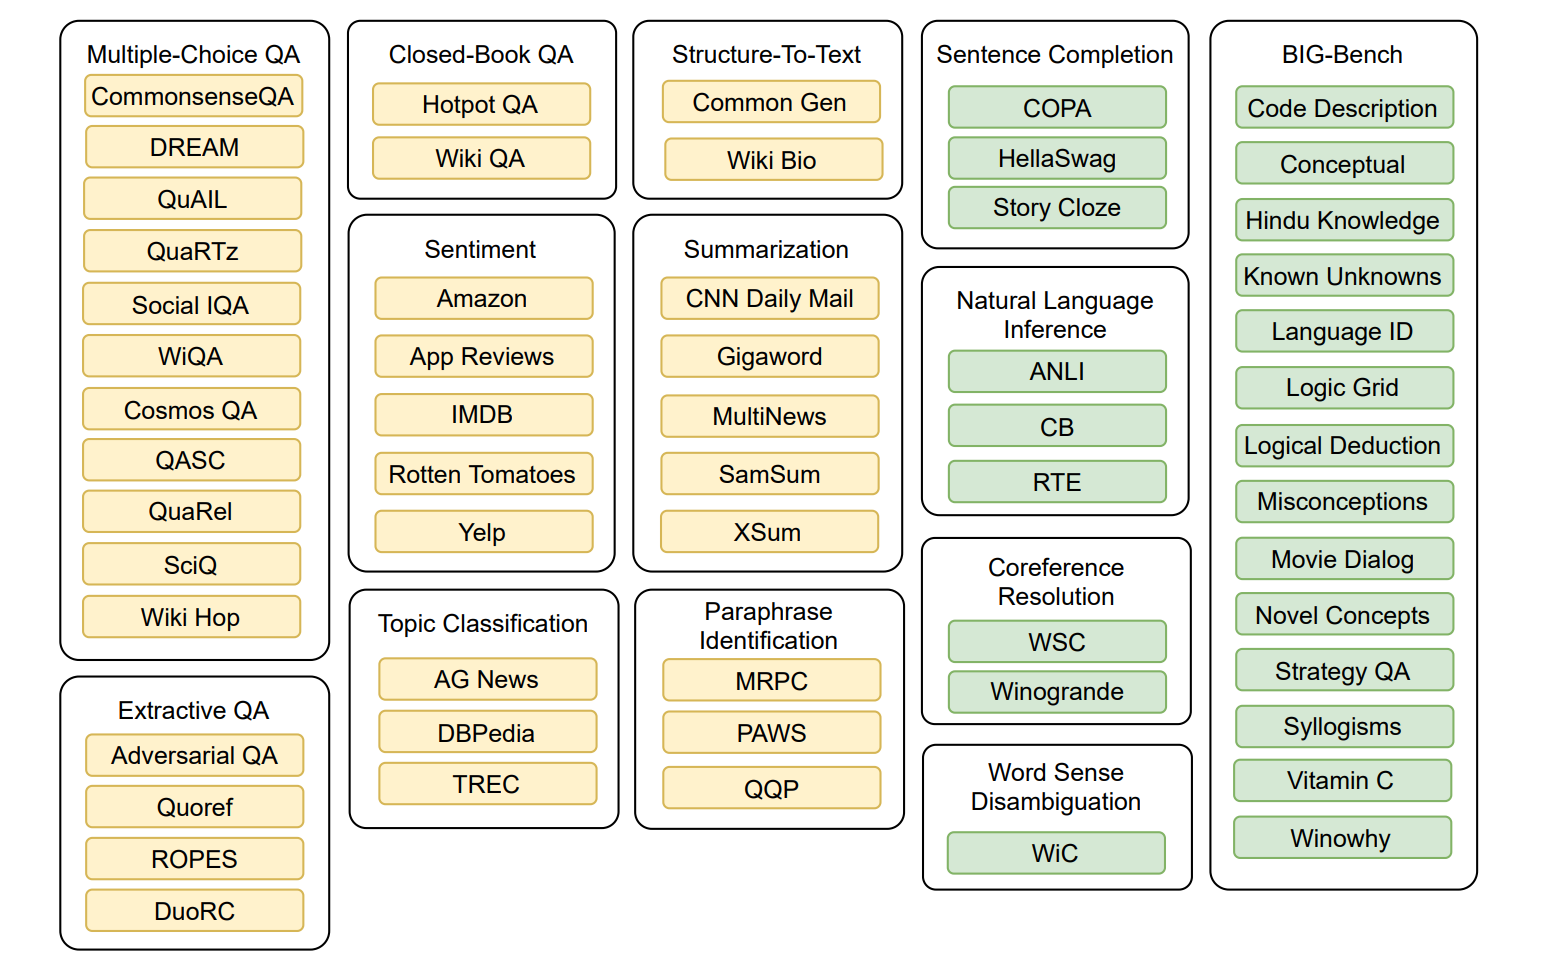
\includegraphics[width = 9.35cm]{figure/81-t0-data.png}\\ 
		\citebutton{Source: Sanh et al.,
		2021}{https://arxiv.org/abs/2110.08207} \ques
		What is an easy task? What is a hard task?
	\end{figure}

\vfill

\end{frame}

% ------------------------------------------------------------------------------

\begin{frame}{t0 -- prompt templates}

\vfill
	
	\begin{figure}
		\centering
		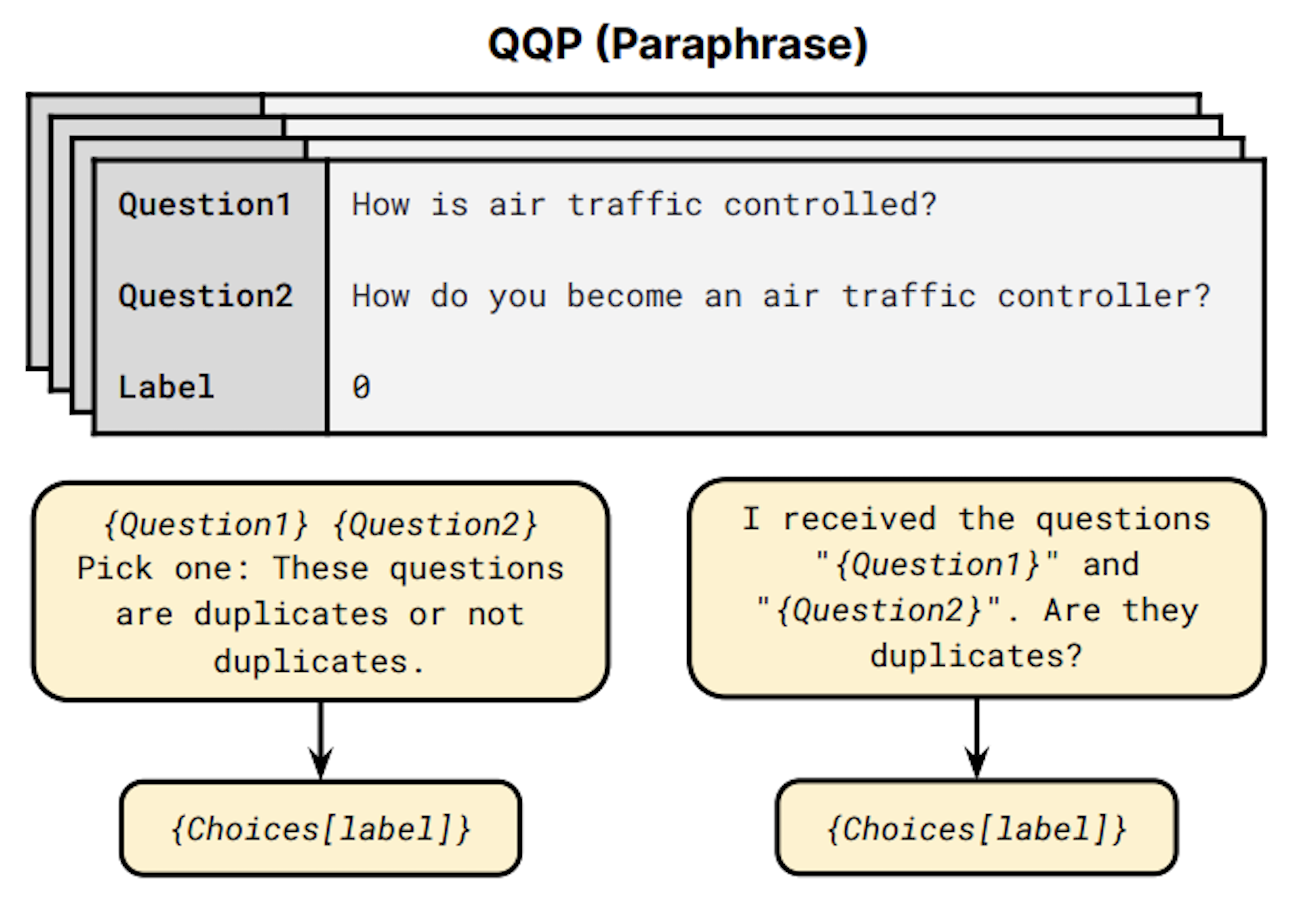
\includegraphics[height=5.95cm]{figure/t0ex1}\\ 
		\citebutton{Source: Sanh et al., 2021}{https://arxiv.org/abs/2110.08207}
	\end{figure}

\vfill

\end{frame}

\begin{frame}{t0 -- prompt templates}

\vfill
	
	\begin{figure}
		\centering
		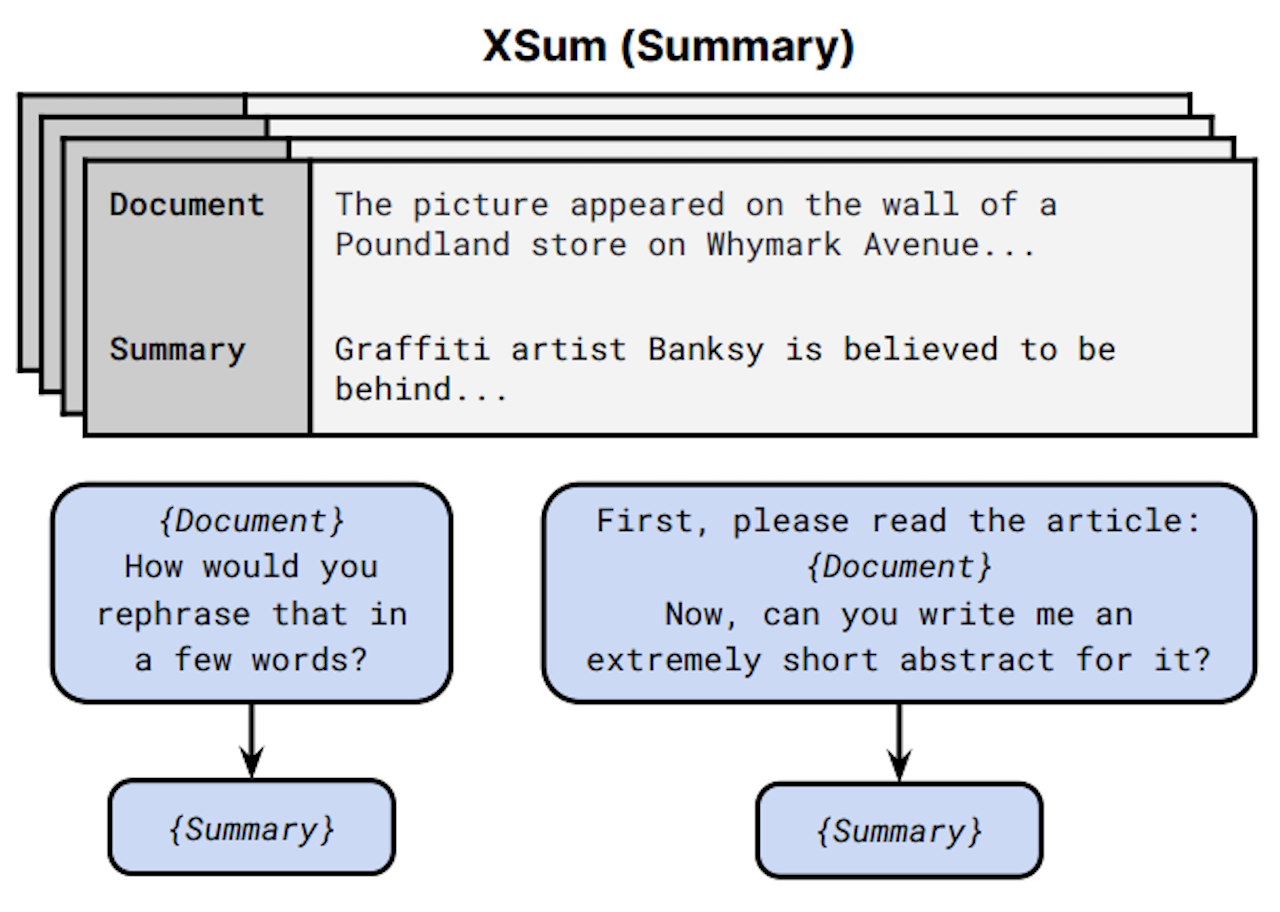
\includegraphics[height=5.95cm]{figure/t0ex2}\\ 
		\citebutton{Source: Sanh et al., 2021}{https://arxiv.org/abs/2110.08207}
	\end{figure}

\vfill

\end{frame}

% ------------------------------------------------------------------------------

\devour{

\begin{frame}{finetuned language net (flan)}

\vfill
	
	\begin{figure}
		\centering
		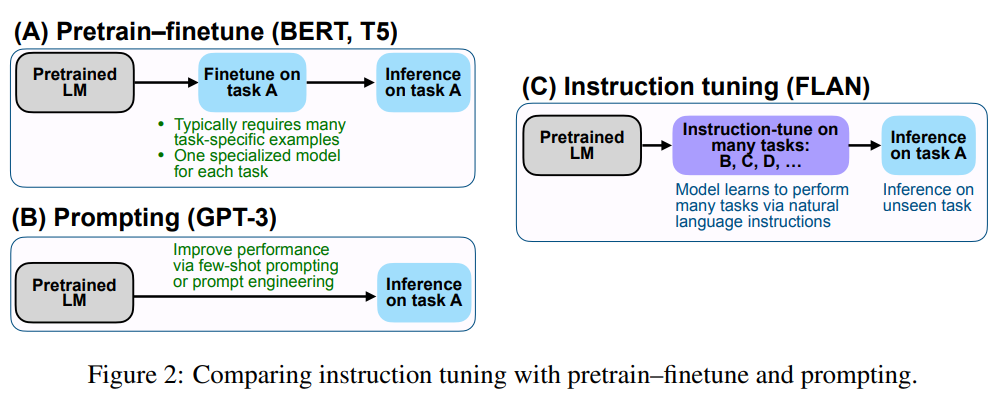
\includegraphics[width = 11cm]{figure/81-flan.png}\\ 
		\citebutton{Source: Wei et al., 2021}{https://arxiv.org/abs/2109.01652}
	\end{figure}

\vfill

\end{frame}
}
% ------------------------------------------------------------------------------

\devour{
\begin{frame}{flan finetuning}

\vfill
	
	\begin{figure}
		\centering
		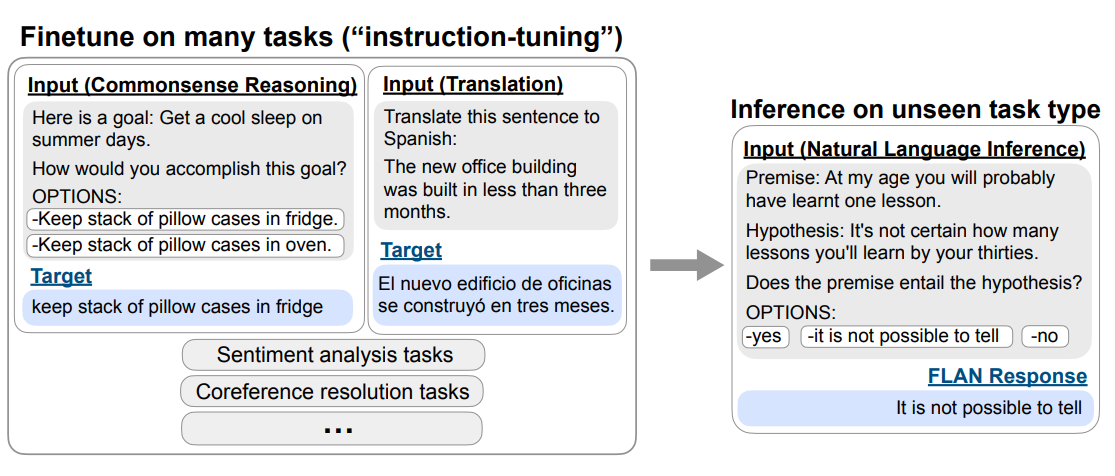
\includegraphics[width = 11cm]{figure/81-flan-instruct-tune.png}\\ 
		\citebutton{Source: Wei et al., 2021}{https://arxiv.org/abs/2109.01652}
	\end{figure}

\vfill

\end{frame}
}
% ------------------------------------------------------------------------------

\begin{frame}{Example of evaluation: flan}

\vfill
	
	\begin{figure}
		\centering
		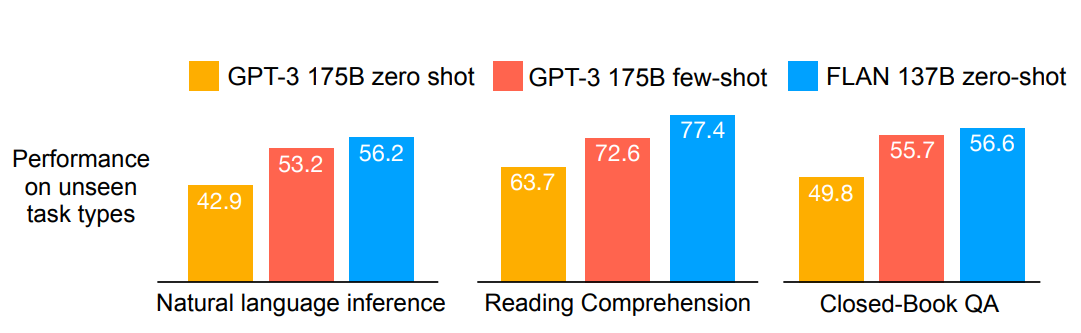
\includegraphics[width = 11cm]{figure/81-flan-perf.png}\\ 
		\citebutton{Source: Wei et al., 2021}{https://arxiv.org/abs/2109.01652}
	\end{figure}

\vfill

\end{frame}

% ------------------------------------------------------------------------------ 

\devour{
\begin{frame}{Extend multi-task learning}

\vfill

\begin{itemize}
\item Scaling the number of tasks and data
  \begin{itemize}
    \item FLAN (1500 tasks, Chung et al., 2022)
    \item NIV2 (1554 tasks)
    \item T0-SF (193 tasks)
    \item Muffin (80 tasks)
    \item CoT (reasoning tasks, cf.\ next chapter)
    \end{itemize}
\item Scaling model sizes
    \begin{itemize}
    \item PaLM 8\,B
    \item PaLM 62\,B
    \item PaLM 540\,B
    \end{itemize}
\end{itemize}

\vfill

\end{frame}
}
% ------------------------------------------------------------------------------ 

\devour{
\begin{frame}{Flan upscaling}

\vfill

\textit{Fine-tuning in 1.8\,K tasks}
    
\begin{figure}
    \centering
    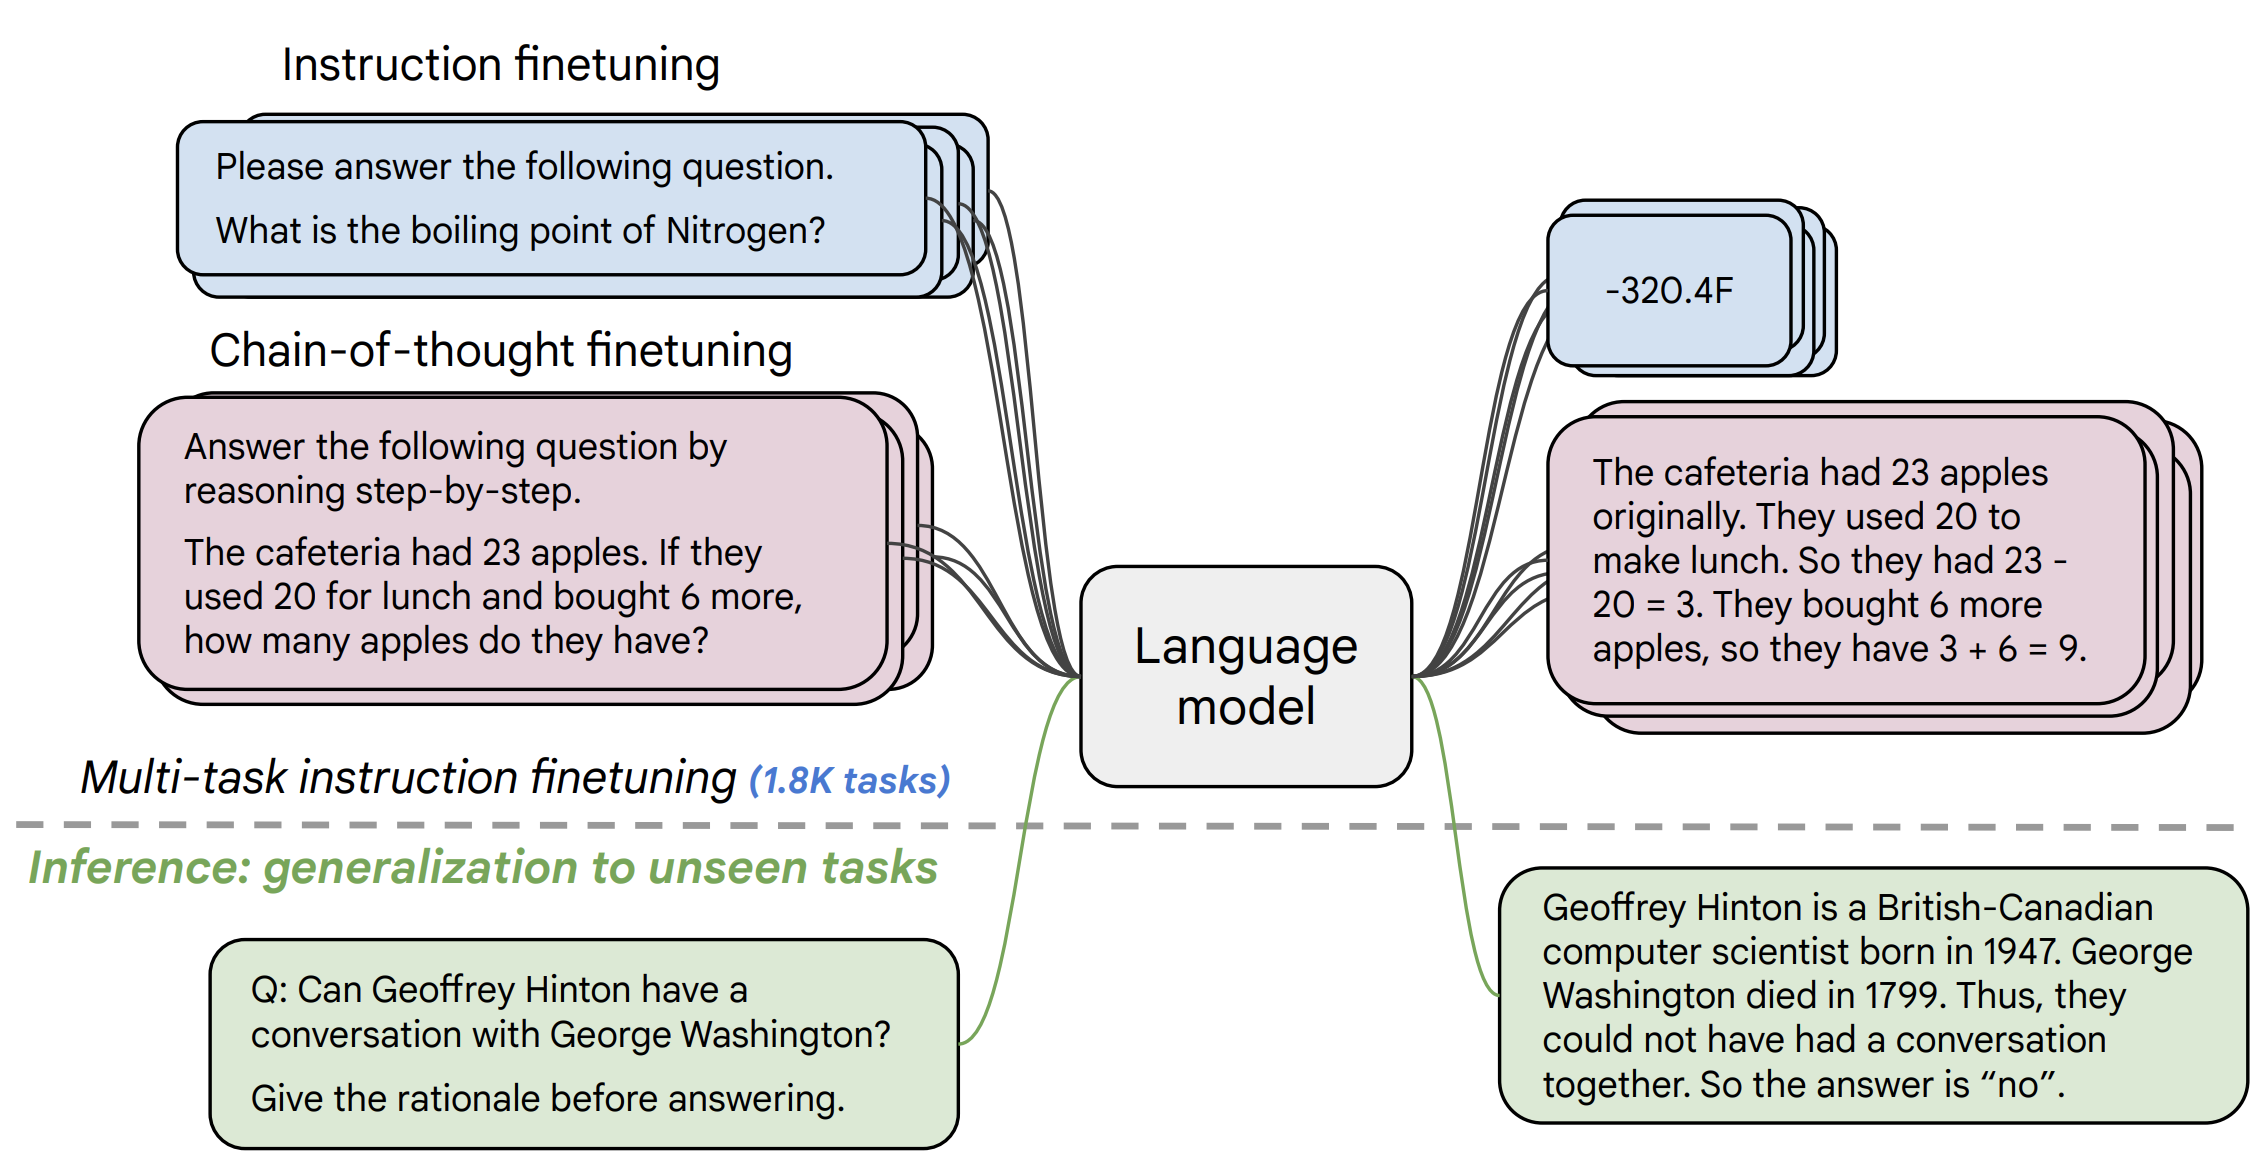
\includegraphics{figure/scaling_up_paradigms.png}\\
\citebutton{Source: Chung et al., 2022}{https://arxiv.org/pdf/2210.11416.pdf}
\end{figure}

\vfill

\end{frame}
}
% ------------------------------------------------------------------------------
\begin{frame}[allowframebreaks]{Multi-task training vs Instruction tuning}
% fit16:9: allowframebreaks instead of shrinking text


\vfill

\begin{itemize}
\item The term ``instruction tuning'' was introduced by FLAN paper,
		\citebutton{Source: Wei et al., 2021}{https://arxiv.org/abs/2109.01652}
\item However, today ``instruction tuning'' refers to a wide
variety of methods that train on instruction-output pairs,
    not just tasks
  \item
    In particular,
open-ended generation and ``alignment'' 
is now included under
    the rubric ``instruction tuning'': brainstorming,
    writing a joke, give me ten analogies for concept X,
    don't use hate language, don't take positions on
    controversial political issues etc
\item These are not classical NLP tasks.
\item See next lecture
\item Our use of terminology in this class:
\item multi-task finetuning = tasks in the classical NLP
    sense
    \item instruction-tuning: a broad approach to changing
    the behavior of a raw language model (i.e., trained on
    next-word prediction) to be ``helpful, harmless and
    honest''. This includes training on classical NLP tasks,
    but it's just one part.
\end{itemize}

\vfill

\end{frame}
% ------------------------------------------------------------------------------

\begin{frame}{Fine-Tuning Conclusions}

\vfill

\begin{itemize}
\item 
     The more training tasks the better
\item Multi-task finetuning generalizes across models
    \begin{itemize}
    \item It works well on different architectures
    \end{itemize}
\item Greatly improves usability
%and mitigates some harms
\item It is relatively compute-efficient
    \begin{itemize}
    \item Pretraining is hugely expensive, finetuning and
    instruction tuning are usually much cheaper.
    \item For PaLM 540\,B it takes 0.2\,\% of pre-training compute, but improves by 9.4\,\%
    \end{itemize}
\end{itemize}

\vfill

\end{frame}

\begin{frame}{Slido}

\vfill

\begin{itemize}
		\item \#1312409 \href{https://app.sli.do/event/egqn27QqTsvFUZPeQvZtVU}{\beamergotobutton{slido}}

%\item \#1312409
\end{itemize}

\vfill

\end{frame}

\devour{

\begin{frame}{T0 vs Flan: Difference?}

\vfill
	
	\begin{figure}
		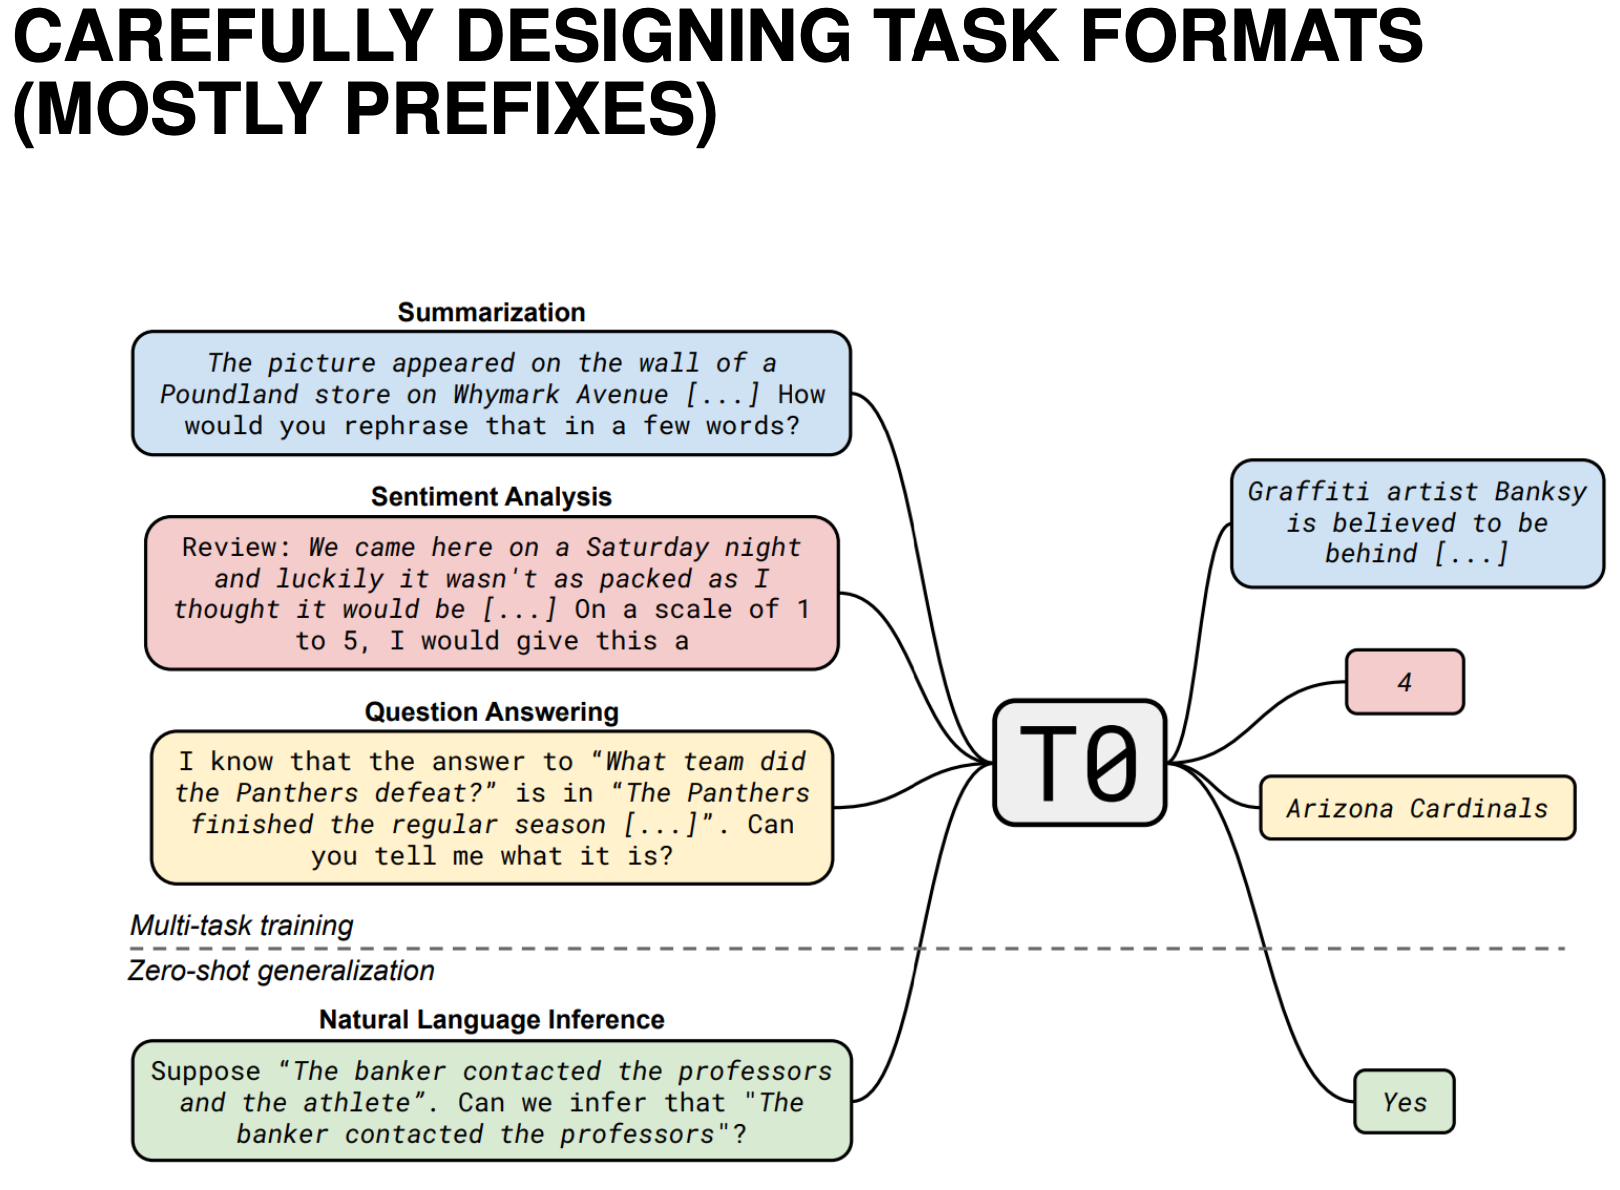
\includegraphics[width=5cm]{figure/t0comparison}
		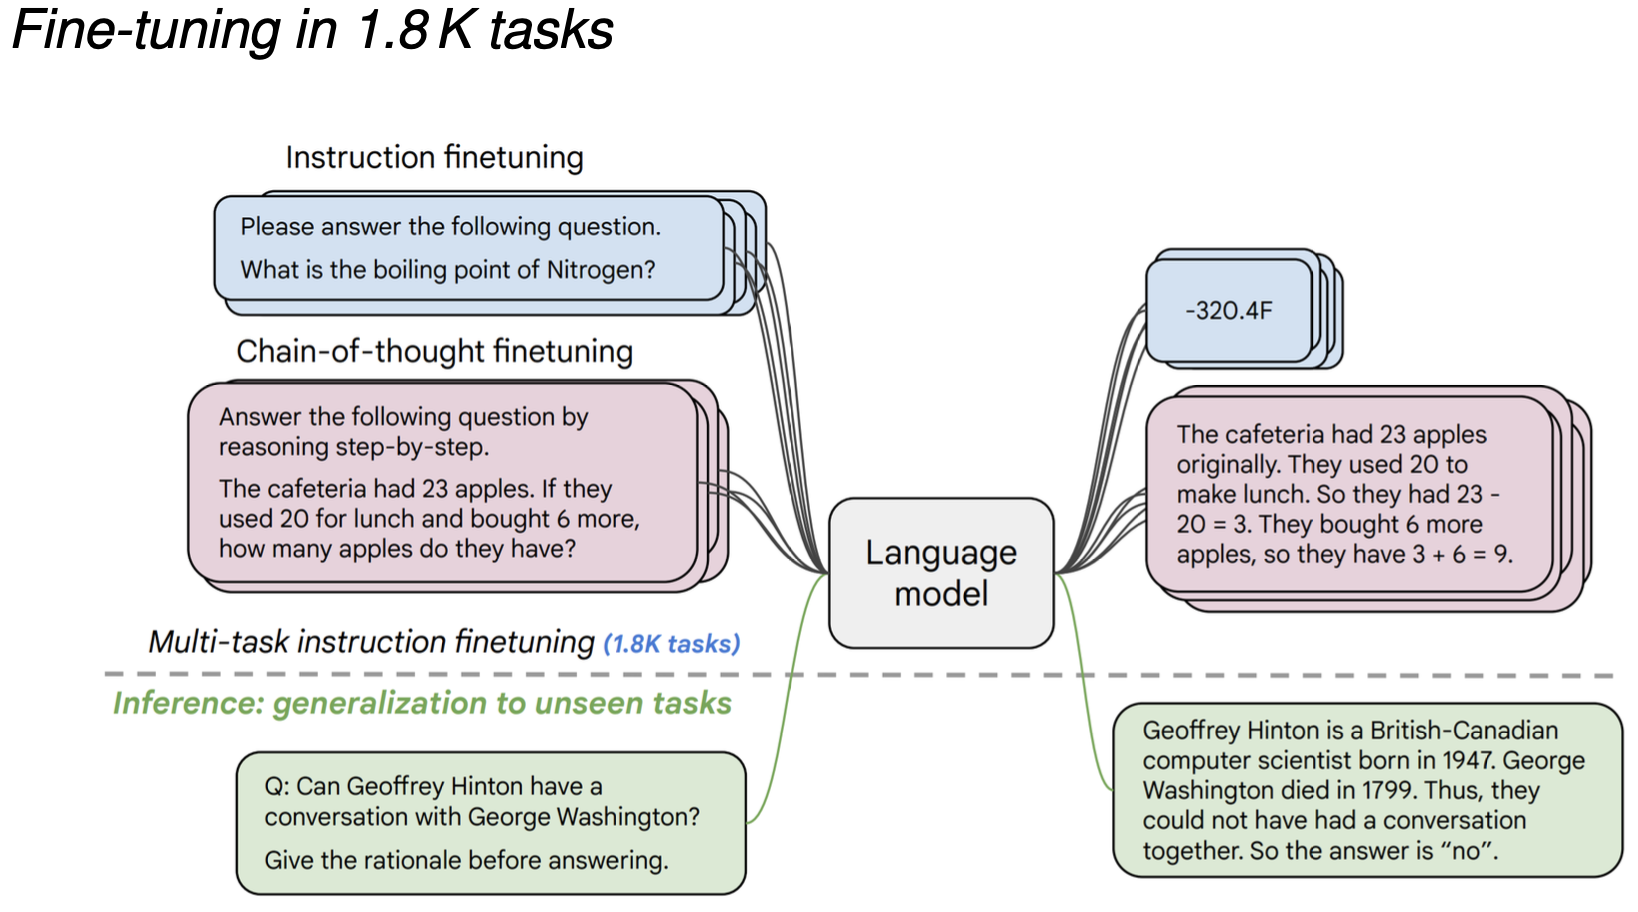
\includegraphics[width=5cm]{figure/flancomparison}
	\end{figure}

\vfill

\end{frame}

}

\def\myblue#1{\textcolor{texblue}{#1}}

\begin{frame}{Prompting: Definition}

\vfill

\begin{itemize}

\item Prompting always means that you \myblue{do not finetune the model},
i.e., you don't change the parameters of the model.

\item The term prompting was initially used for when you \myblue{carefully design the
input to the language model}, so that you will get the
desired output.

\item \myblue{But nowadays any type of input to the model can be called
a prompt.}

\item \myblue{Few-shot or k-shot prompting} means that you give a few
examples or k examples of what you want the model to do
as part of the input to the model.

\item \myblue{Zero-shot prompting} means that you do not give an example.
The term zero-shot prompting is often used in the context of
few-shot prompting (contrasting using $k>0$ examples vs $k=0$
examples).

\end{itemize}

\vfill

\end{frame}


%%%%%%%%%%%%%%%%%%%%%%%%%%%%%%%%%%%%%%%%%%%%%%%%%%%%%%%%%%%%%%%%%%
\section{Chain-of-Thought Few-Shot Prompting}
% Source: DL4NLP chapter09-llm/slides-92-chain-of-thought.tex
%%%%%%%%%%%%%%%%%%%%%%%%%%%%%%%%%%%%%%%%%%%%%%%%%%%%%%%%%%%%%%%%%%
%\lecturechapter{Large Language Models (LLMs)}




\begin{frame}[allowframebreaks]{\cotpfullcap motivation}
% fit16:9: allowframebreaks instead of shrinking text


\vfill

How to boost the reasoning capabilities of LMs? \citebutton{Wei et al., 2021}{https://arxiv.org/abs/2109.01652}

\begin{itemize}
\item Use formal approaches, e.g., logic, symbolic reasoning
    \begin{itemize}
    \item Example: \citebutton{BeliefBank}{https://arxiv.org/abs/2109.14723}
\item Difficult to train and deploy, not widely used
    \end{itemize}
\item Standard few-shot learning via prompting works for many tasks
    \begin{itemize}
    \item Still, it works poorly for many tasks that require reasoning
    \end{itemize}
\item \cotp
    \begin{itemize}
    \item A form of few-shot prompting
    \item Each ``training example'' has the form:\\ <input, \textit{chain of thought}, output>
    \item chain of thought:\\ series of reasoning steps that
    lead to the final answer
  \item application:
    reasoning tasks:
    complex, commonsense, symbolic etc
    \end{itemize}

\end{itemize}

\vfill

\end{frame}

\begin{frame}{Neurosymbolic approach\\ (currently
    infrequently used)}

\vfill
	
	\begin{figure}
		\centering
		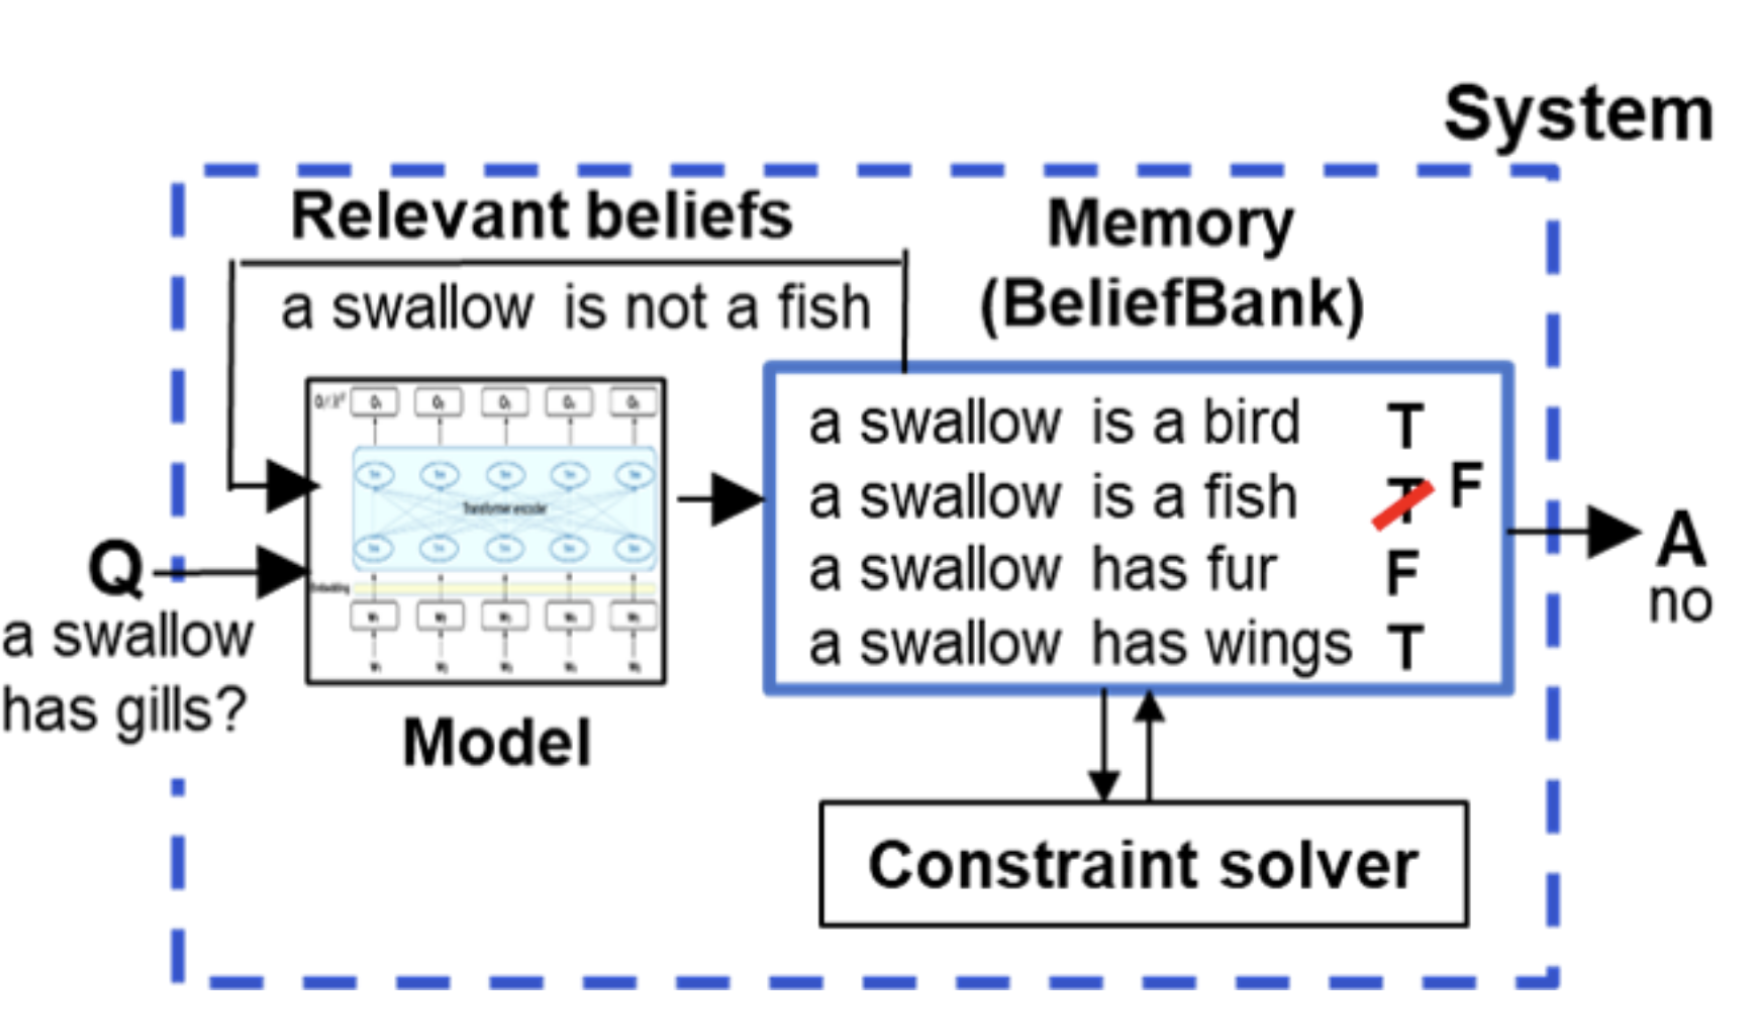
\includegraphics[height = 6cm]{figure/beliefbank} 
	\end{figure}

\vfill

\end{frame}


\begin{frame}{LMs not good at reasoning tasks\\ (This is
    why we need \cotp.)}

\vfill
	
	\begin{figure}
		\centering
		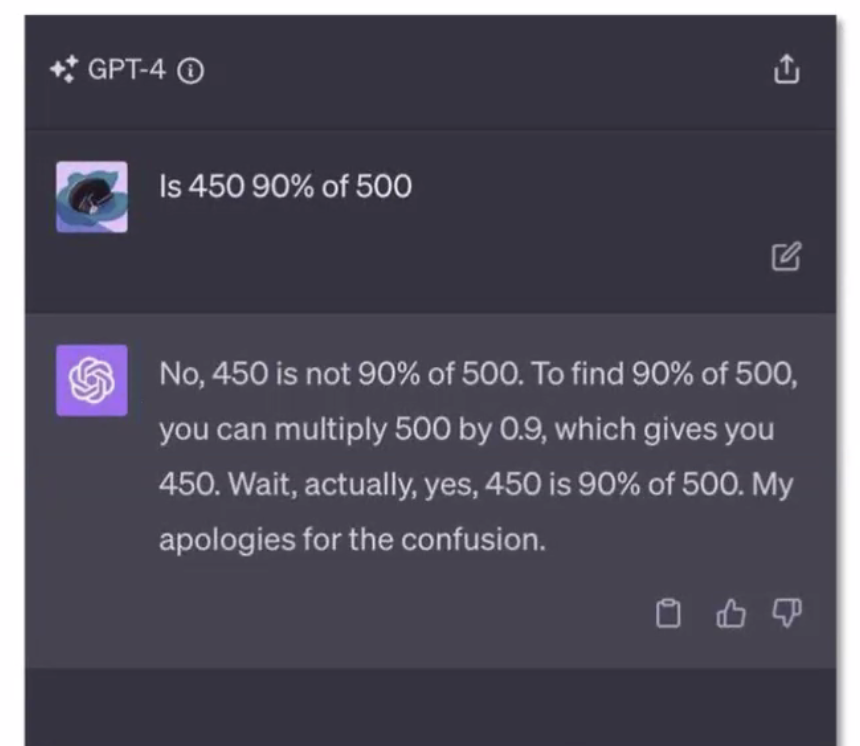
\includegraphics[height = 5.10cm]{figure/is450,90,of,500} 
	\end{figure}

\ques What is the problem here?
% left-to-right next-token prediction

\vfill

\end{frame}


% ------------------------------------------------------------------------------ 

\begin{frame}{\cotpfullcap paradigm}

\vfill

%\textbf{\cotp enables LLMs to tackle complex arithmetic, commonsense and symbolic reasoning tasks.}

\begin{figure}
    \centering
    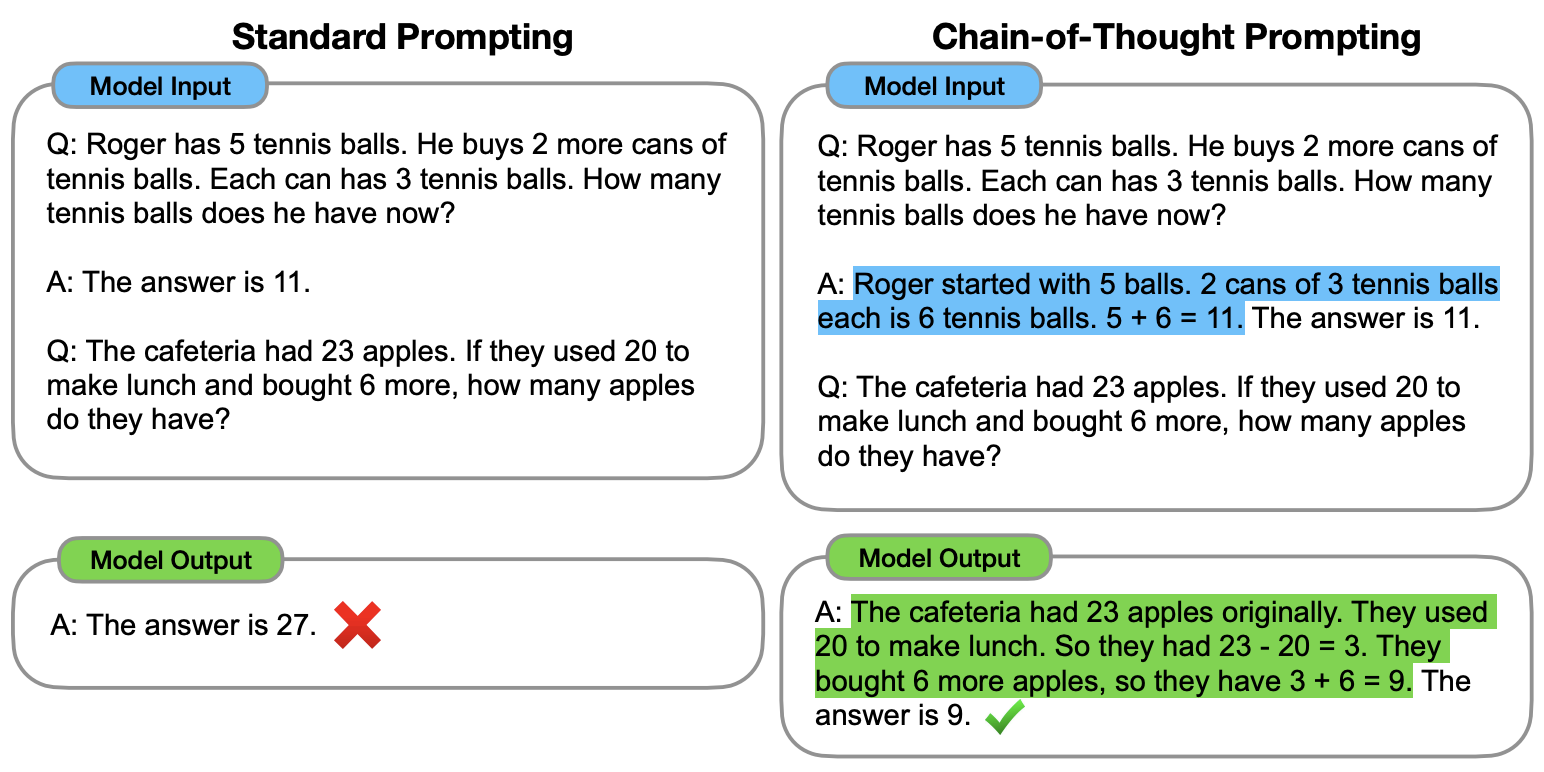
\includegraphics{figure/chain_of_thought.png}\\
    \citebutton{Source: Wei et al., 2022}{https://arxiv.org/pdf/2201.11903.pdf}
\end{figure}

\vfill

\end{frame}

% ------------------------------------------------------------------------------ 

\begin{frame}{\cotpfull paradigm}

\begin{figure}
    \centering
    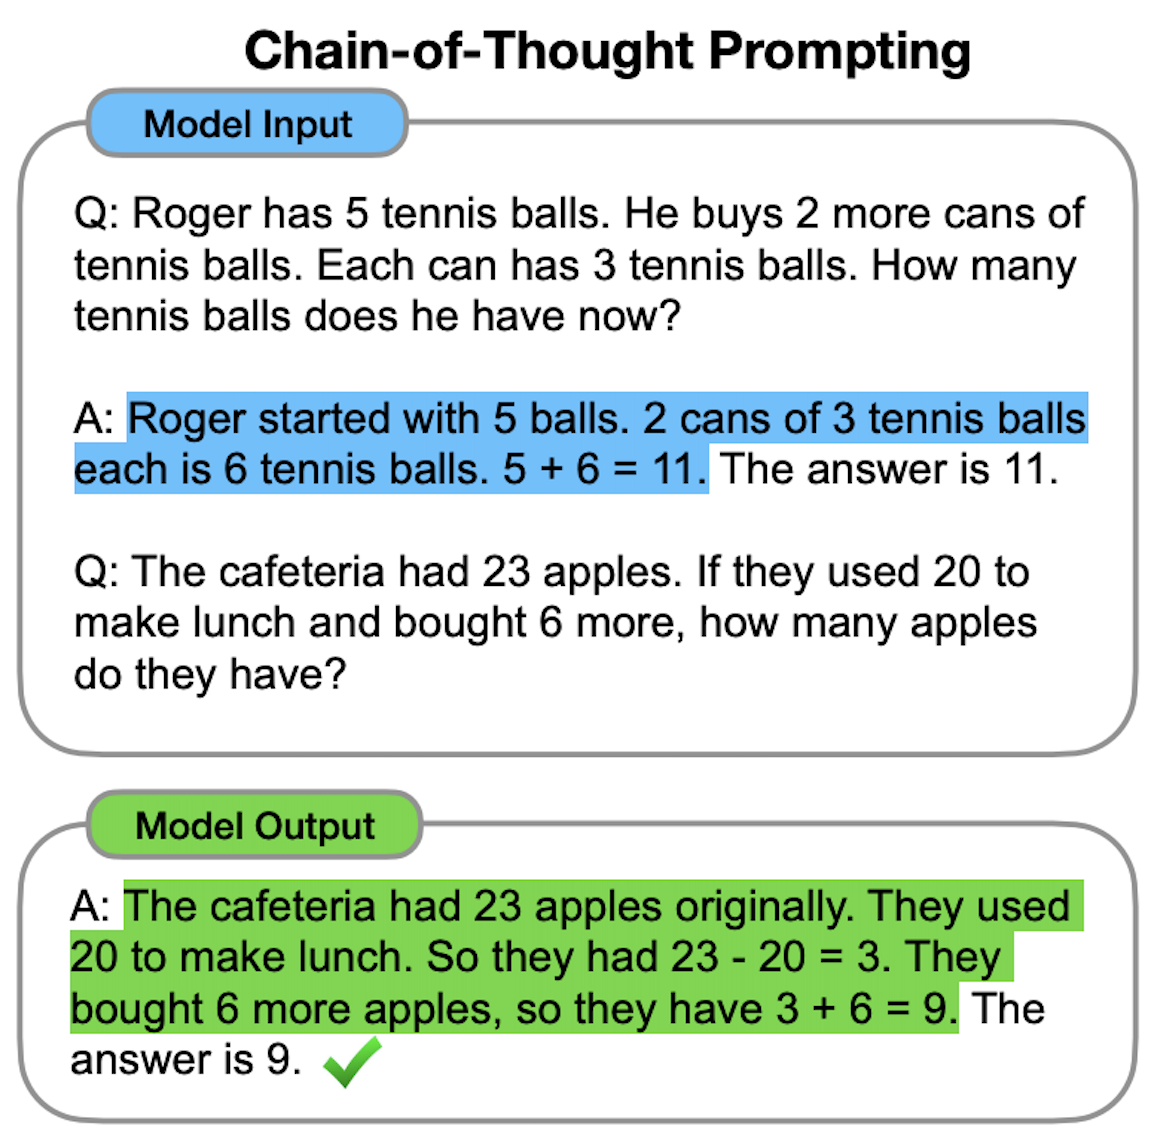
\includegraphics[height=5.95cm]{figure/chain_of_thought2.png}
\end{figure}

\end{frame}

% ------------------------------------------------------------------------------


\begin{frame}{Benefits of \cotpfull}

\vfill

\begin{itemize}
    \item Decompose multi-step problems and thus allocate more compute to problems requiring more reasoning steps.
    \item This helps LMs 
    solve problems they otherwise would not be able to solve.
    \item By describing the reasoning, interpretability is increased. It provides the possibility to observe where reasoning went wrong
    \item \cotp  is closer to how humans solve tasks using language
\end{itemize}

\vfill

\end{frame}


% ------------------------------------------------------------------------------

\begin{frame}{\cotpfull}

\vfill

\textbf{Following slides: Examples of $<$input, chain of thought, output$>$ triples for  commonsense and symbolic reasoning}

    \citebutton{Source: Wei et al., 2022}{https://arxiv.org/pdf/2201.11903.pdf}

The few shots (training examples) are omitted from these
examples to save space, but this is
\cotpfull,
 that is, the model is prompted with examples of
chain of thought reasoning.


\vfill

\end{frame}

% ------------------------------------------------------------------------------

\begin{frame}{Examples}

\vfill

\begin{figure}
    \centering
    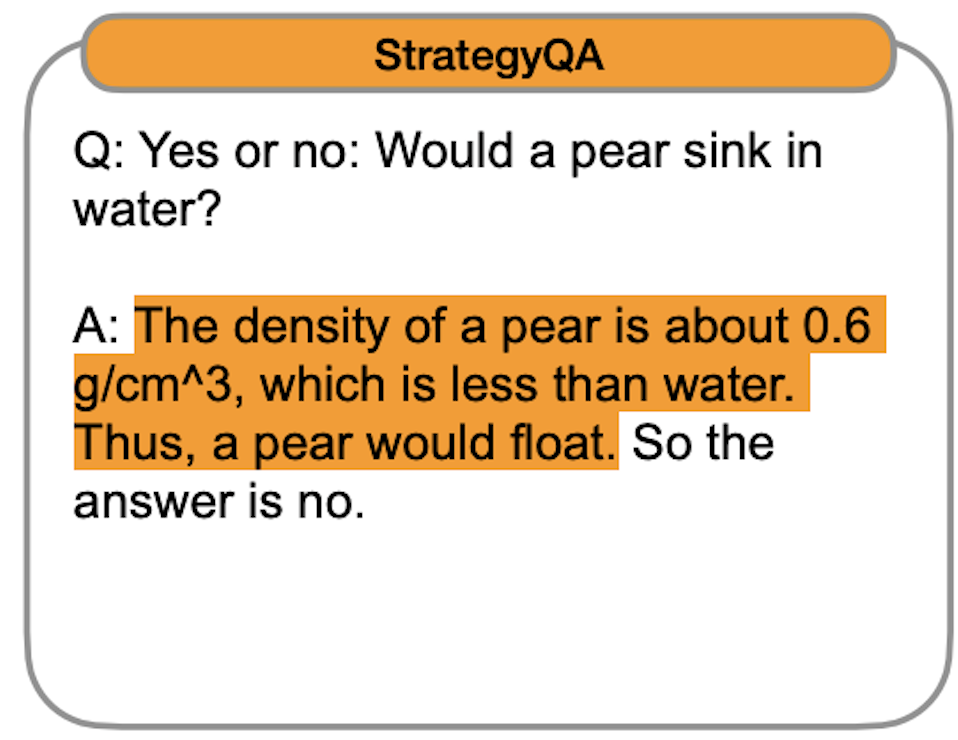
\includegraphics[height=5.95cm]{figure/cotex1.png}
\end{figure}

\vfill

\end{frame}

\begin{frame}{Examples}

\vfill

\begin{figure}
    \centering
    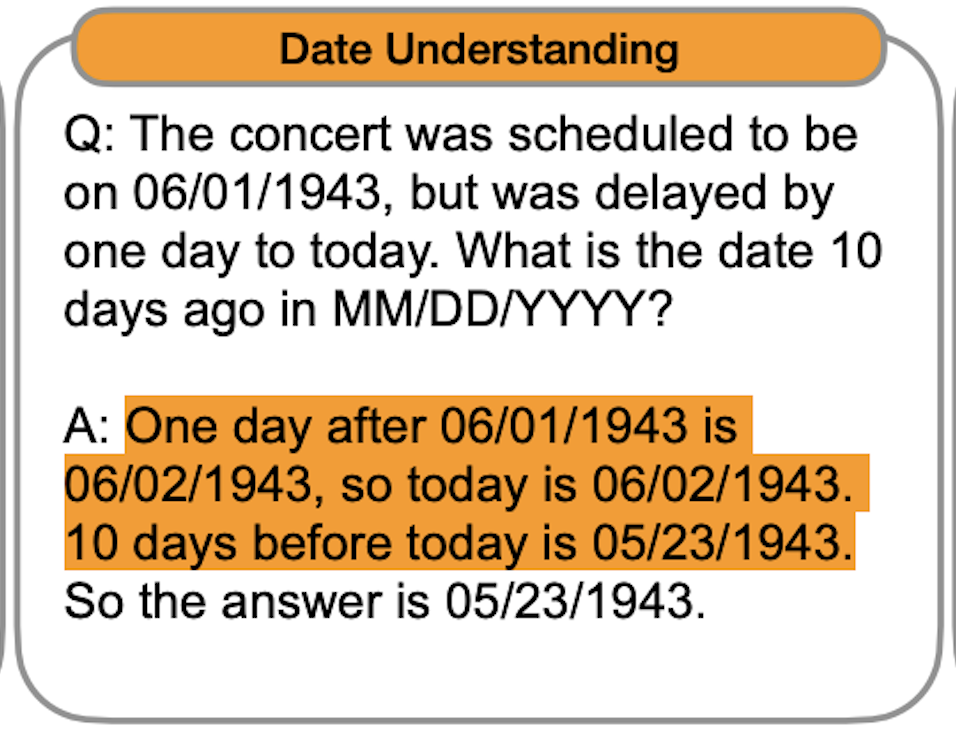
\includegraphics[height=5.95cm]{figure/cotex2.png}
\end{figure}

\vfill

\end{frame}

\begin{frame}{Examples}

\vfill

\begin{figure}
    \centering
    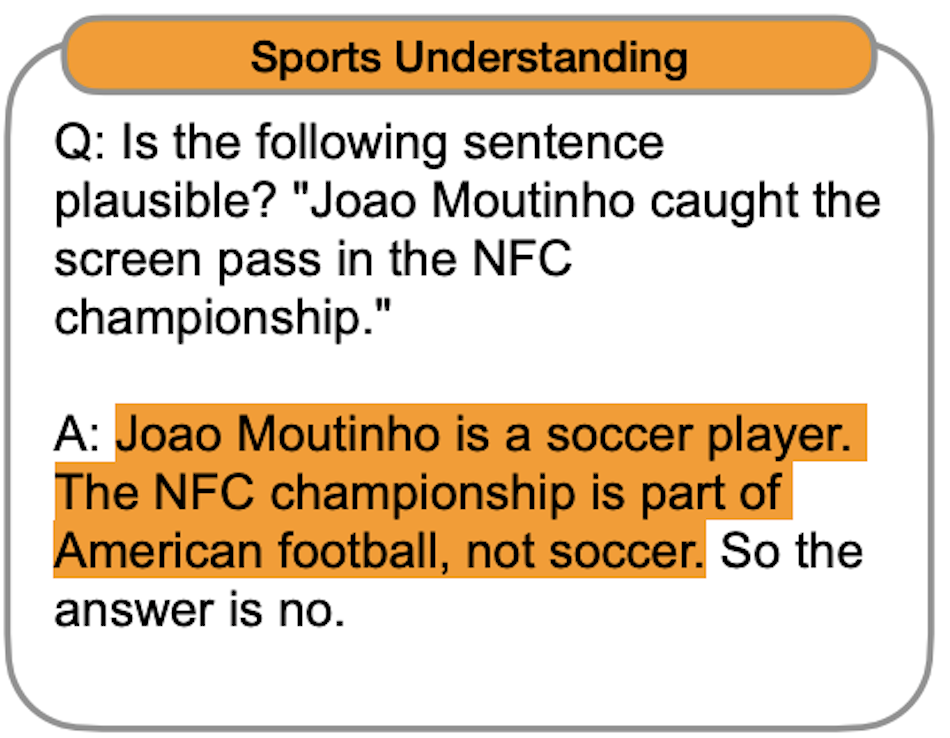
\includegraphics[height=5.95cm]{figure/cotex3.png}
\end{figure}

\vfill

\end{frame}

\begin{frame}{Examples}

\vfill

\begin{figure}
    \centering
    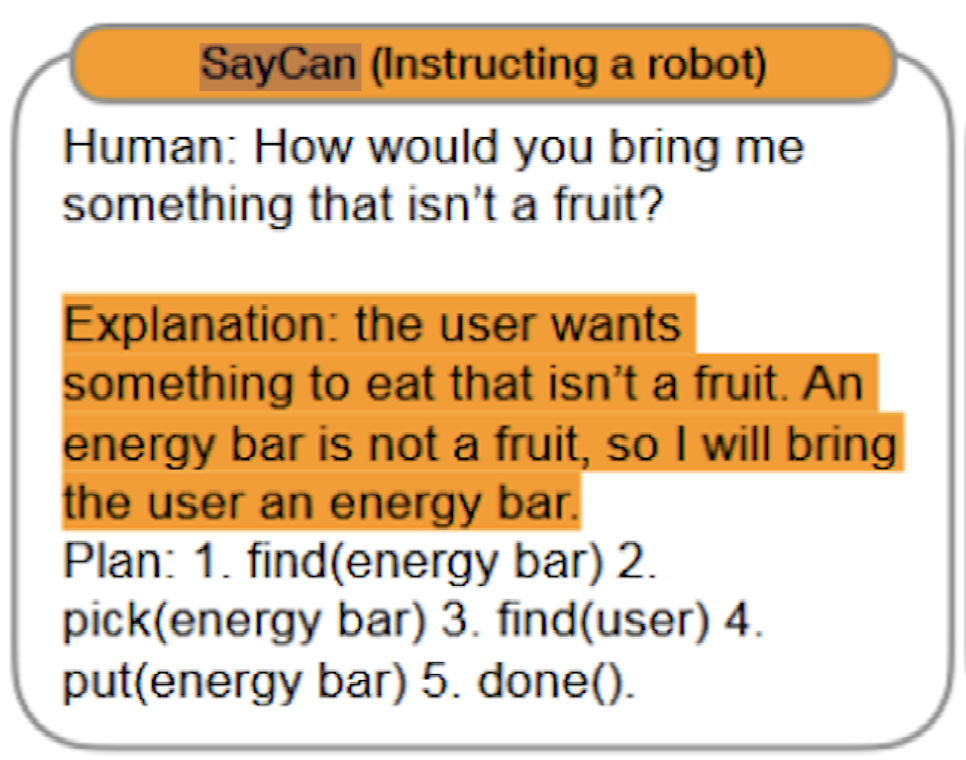
\includegraphics[height=5.95cm]{figure/cotex4.png}
\end{figure}

\vfill

\end{frame}

\begin{frame}{Examples}

\vfill

\begin{figure}
    \centering
    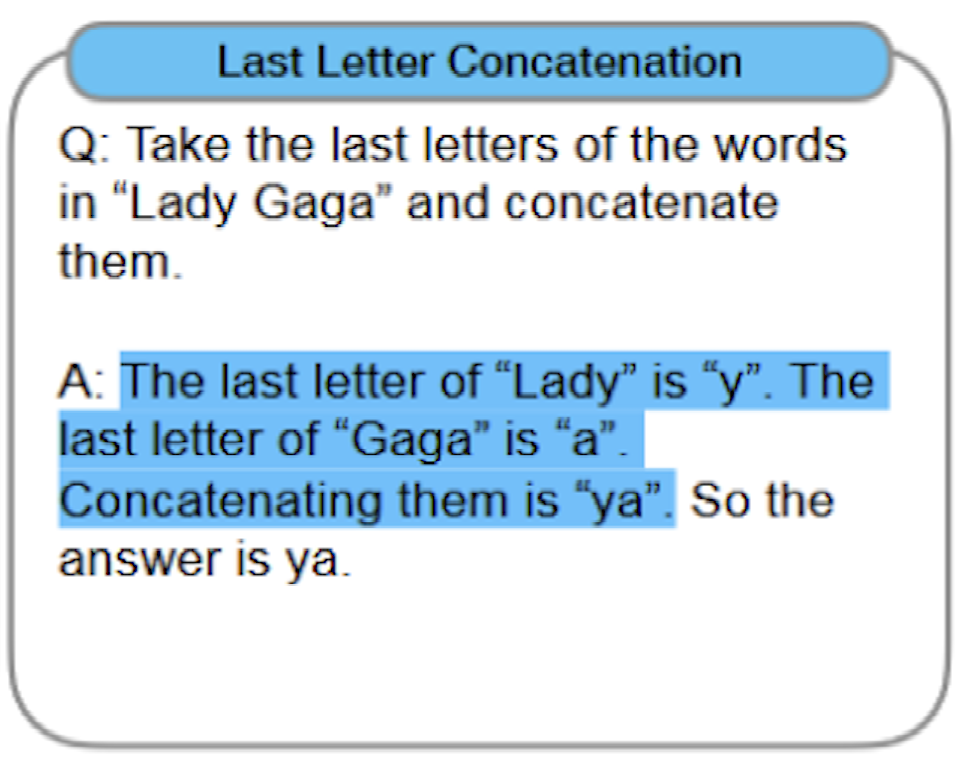
\includegraphics[height=5.95cm]{figure/cotex5.png}
\end{figure}

\vfill

\end{frame}

\begin{frame}{Examples}

\vfill

\begin{figure}
    \centering
    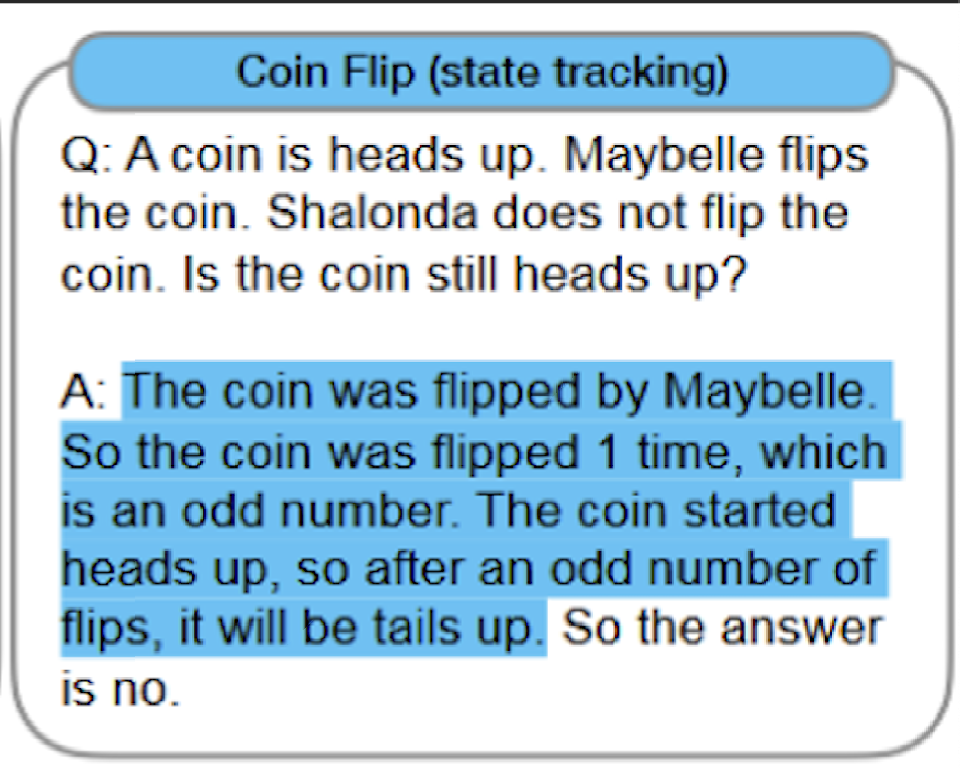
\includegraphics[height=5.95cm]{figure/cotex6.png}
\end{figure}

\vfill

\end{frame}

% ------------------------------------------------------------------------------

\begin{frame}{\cotp improves arithmetic}

\vfill
	
	\begin{figure}
		\centering
		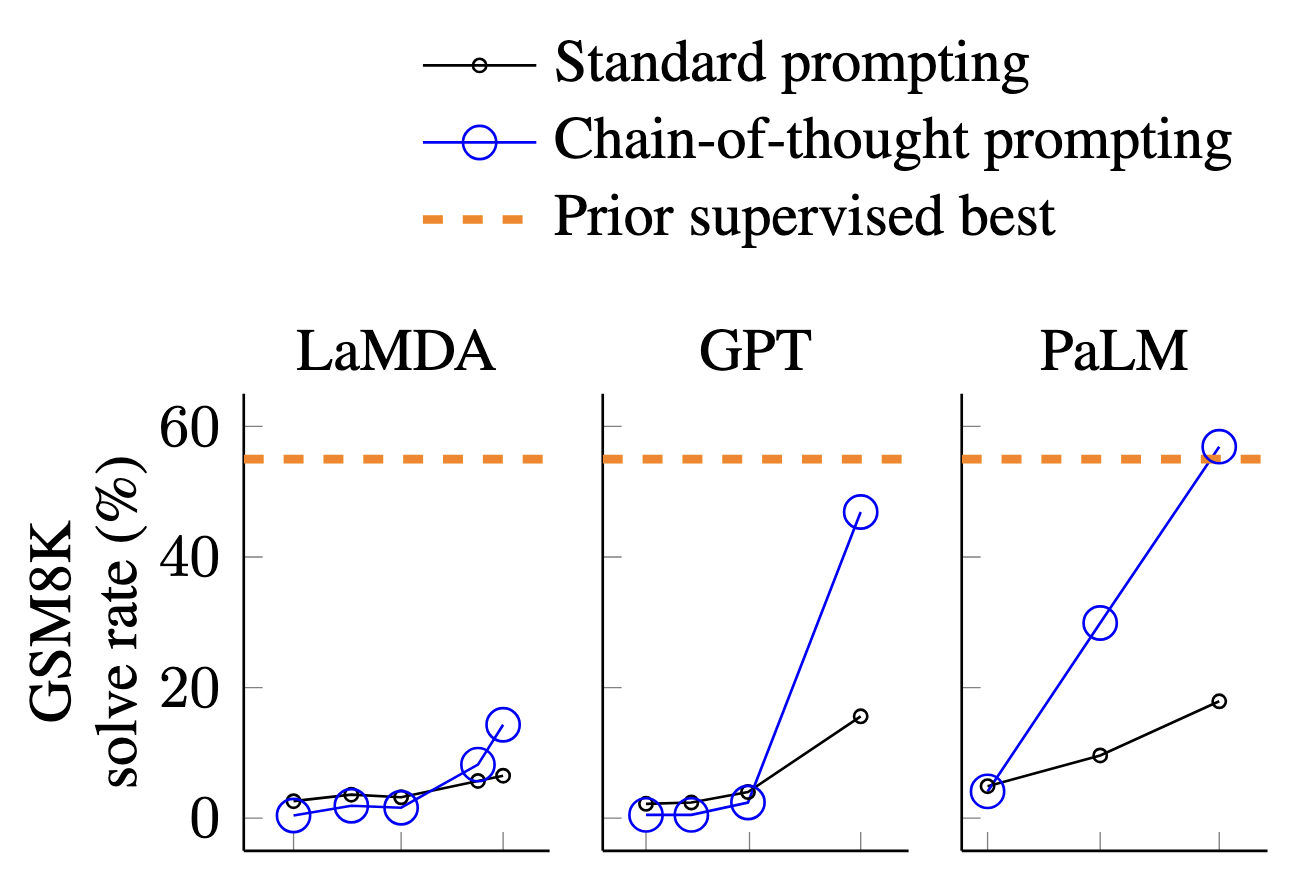
\includegraphics[height = 5.95cm]{figure/cotperformance} 
	\end{figure}

\vfill

\end{frame}


\begin{frame}{\cotp improves arithmetic}

%\vfill

SVAMP: math word problems with varying structures; MAWPS:
repository unifying math problems from different sources;
    \citebutton{Source: Wei et al., 2022}{https://arxiv.org/pdf/2201.11903.pdf}

\begin{figure}
    \centering
    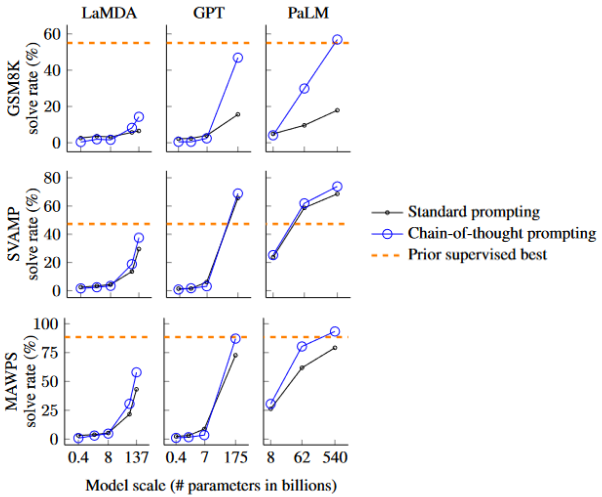
\includegraphics[width=0.6\textwidth]{figure/cot_performance1.png}
\end{figure}

%\vfill

\end{frame}

% ------------------------------------------------------------------------------
\begin{frame}{\cotp improves commonsense}

\vfill

\devour{CSQA: Contains around 200K dialogs with a total of 1.6M
turns. Further, unlike existing large scale QA datasets
which contain simple questions that can be answered from a
single tuple, the questions in the dialogs require a larger
subgraph of the KG. }


\begin{figure}
    \centering
    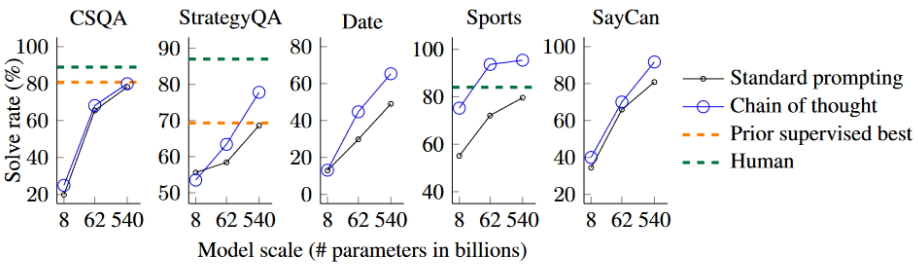
\includegraphics[width=0.9\textwidth]{figure/cot_performance2.png}\\
    \citebutton{Source: Wei et al., 2022}{https://arxiv.org/pdf/2201.11903.pdf}
\end{figure}

\vfill

\end{frame}

%\endlecture
%


%%%%%%%%%%%%%%%%%%%%%%%%%%%%%%%%%%%%%%%%%%%%%%%%%%%%%%%%%%%%%%%%%%
\section{Emergent Abilities}
% Source: DL4NLP chapter09-llm/slides-93-emergent-abilities.tex
%%%%%%%%%%%%%%%%%%%%%%%%%%%%%%%%%%%%%%%%%%%%%%%%%%%%%%%%%%%%%%%%%%
% ------------------------------------------------------------------------------

\begin{frame}{Emergent abilities}

\vfill

An \textit{emergent ability} is an ability that is not
present in small models but is present in large models.
\vskip3mm

\begin{itemize}
\item Assumption: Everything else is held constant.
    \item Questions: Is emergence a rare phenomenon?
    Are many tasks emergent?
    \item We can answer this by investigating model families
    with many sizes.
    \begin{itemize}
        \item GPT-3
        \item Chinchilla
        \item PaLM
    \end{itemize}
\end{itemize}

\vfill

\end{frame}

% ------------------------------------------------------------------------------

\begin{frame}{Emergent abilities and model size}

\vfill

\begin{figure}
    \centering
    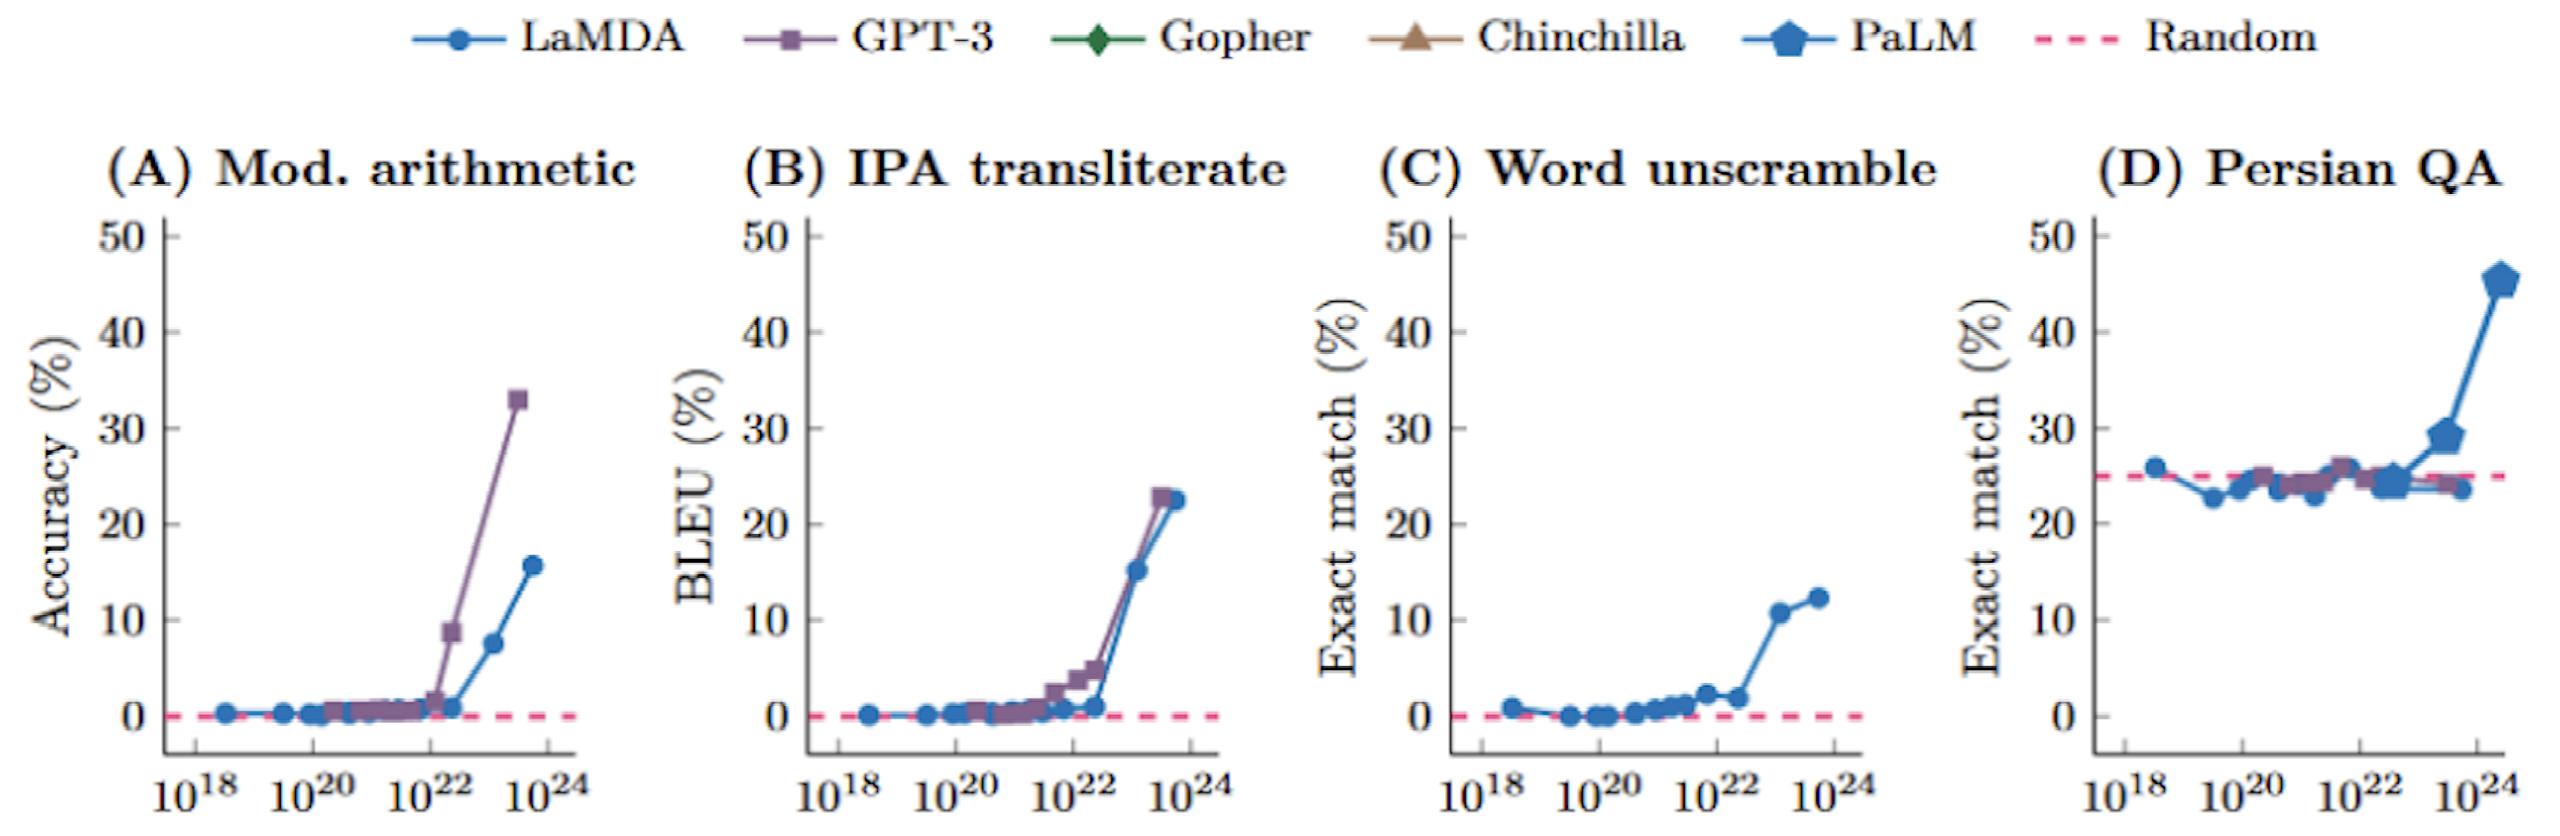
\includegraphics[width=13cm]{figure/emergent_abilities2.png}
    \caption{Examples of emergence in few-shot prompting. \citebutton{Wei et al., 2022}{https://arxiv.org/abs/2206.07682}}
\end{figure}

\vfill

\end{frame}
\begin{frame}{Emergent abilities and model size}

\vfill

\begin{figure}
    \centering
    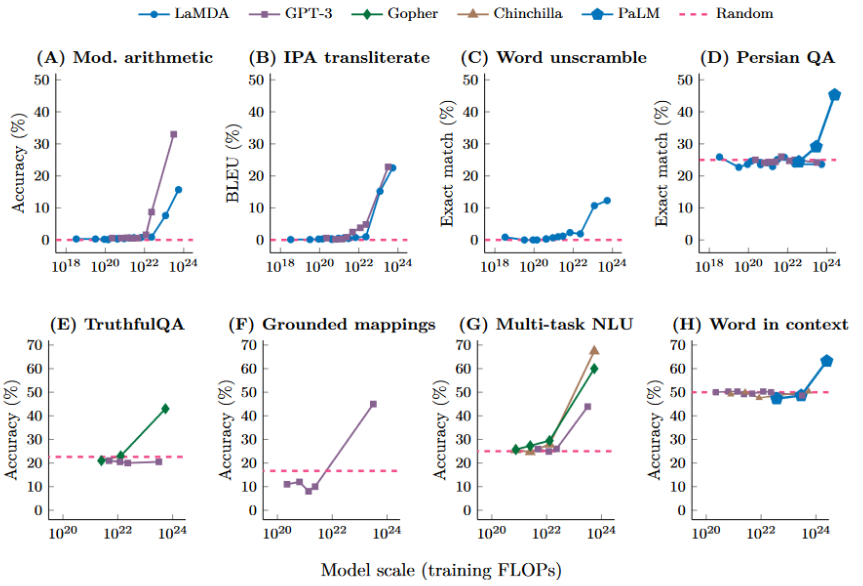
\includegraphics[width=0.71\textwidth]{figure/emergent_abilities.png}
    \caption{Examples of emergence in few-shot prompting. \citebutton{Wei et al., 2022}{https://arxiv.org/abs/2206.07682}}
    \label{fig:emergent_abilities}
\end{figure}

\vfill

\end{frame}

% ------------------------------------------------------------------------------

\begin{frame}{Emergent tasks in Big-Bench}

\vfill

\begin{itemize}
\item ``MODEL SIZE (TASK)'' means: MODEL can do
TASK with SIZE, but not with less than SIZE (hence emerging)
    \item GPT-3 13B (2 tasks): hindu knowledge, modified arithmetic
    \item GPT-3 175B (15 tasks): analytic entailment, codenames, phrase relatedness, question answer creation, self evaluation tutoring, ...
    \item LaMDA 137B (8 tasks): gender inclusive sentences german, repeat copy logic, sports understanding, ...
    \item PaLM 8B (3 tasks): auto debugging, sufficient information, ParsiNLU reading comprehension
    \item PaLM 64B (14 tasks): anachronisms, ascii word recognition, conceptual combinations, ...
    \item PaLM 540B (25 tasks): analogical similarity, causal judgment, code line description, crass ai, cs algorithms, ...
\end{itemize}

\vfill

\end{frame}

% ------------------------------------------------------------------------------

\begin{frame}{Emergent tasks in MMLU}

\vfill

\begin{itemize}
    \item Chinchilla 7B (7 tasks): Professional Medicine, High School Statistics, High School Macroeconomics, High School Psychology, Anatomy, High School Government And Politics, High School Microeconomics
    \item Chinchilla 70B (44 tasks): International Law, Human Aging, Sociology, Us Foreign Policy, High School World History, Marketing, Logical Fallacies, Miscellaneous, College Biology, High School Us History, Security Studies, High School European History, ...
\end{itemize}

\vfill

\end{frame}

% ------------------------------------------------------------------------------

\begin{frame}{Other emergent tasks}

\vfill

\begin{itemize}
    \item GPT-3 paper: 3 digit addition/subtraction (GPT-3 13B), 4-5 digit addition/substraction (GPT-3 175B), leveraging few-shot examples for word denoising (GPT-3 13B)
    \item Gopher paper: Toxicity classification (Gopher 7.1B), TruthfulQA (Gopher 280B)
    \item Patel \& Pavlick: grounded conceptual mappings (GPT-3 175B)
    \item PaLM paper: Word in Context benchmark (PaLM 540B)
\end{itemize}

\vfill

\end{frame}

% ------------------------------------------------------------------------------

% \begin{frame}{Impact of Model Size}

% \vfill

% \vfill

% \end{frame}

% ------------------------------------------------------------------------------

\begin{frame}{counter argument}

\citebutton{Source: Schaeffer et al., 2023}{https://arxiv.org/pdf/2304.15004.pdf}

\vfill

Two defining properties for emergent abilities in LLMs:

\begin{enumerate}
%
\item \textbf{Sharpness:} transitioning seemingly instantaneously from not present to present
%
\item \textbf{Unpredictability:} transitioning at seemingly unforeseeable model scales
%
\end{enumerate}

\vskip5mm

Claim: Emergent abilities appear only under metrics that nonlinearly or discontinuously scale model's per-token error rate:

	\begin{figure}
		\centering
		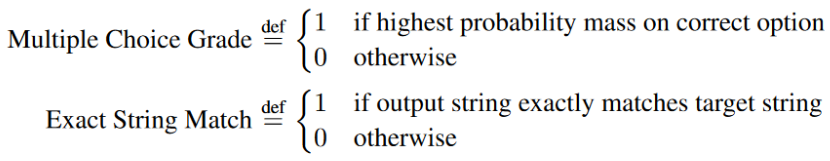
\includegraphics[width = 11cm]{figure/metrics.png} \\ 
	\end{figure}

\vfill

\end{frame}

% -----------------------------------------------------------------------------

\begin{frame}{counter argument}

\vfill

	\begin{figure}
		\centering
		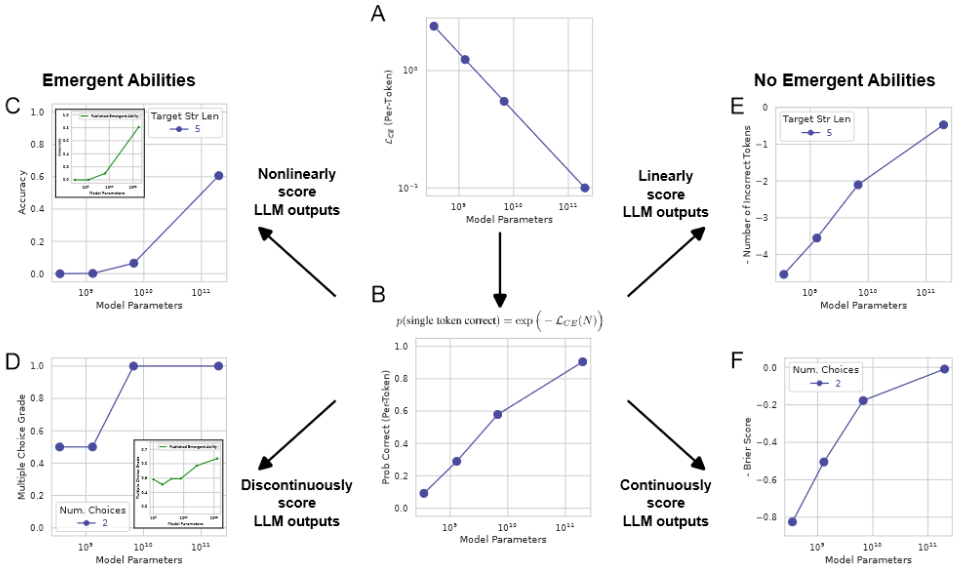
\includegraphics[width = 9.35cm]{figure/emergent_experiments.png}\\ 
		\citebutton{Source: Schaeffer et al., 2023}{https://arxiv.org/pdf/2304.15004.pdf}
	\end{figure}

\vfill

\end{frame}

% ------------------------------------------------------------------------------

\begin{frame}{Counterargument: Summary}

\vfill

%\textbf{Conclusions:}
%
\begin{itemize}
%
\item \myblue{Emergence is merely an artifact of the evaluation
		measures we use.}

\item
If TASK is emergent for family MODEL at SIZE on METRIC, then
it is often possible to choose another metric for which the
task is not emergent.
%
\item Emergent abilities can be induced in computer vision tasks as well
%
\item A task and a metric are distinct and meaningful choices when constructing a benchmark
%
\item When choosing a metric, one should consider the
metric's effect on the per-token error rate;
may require adapting the measuring process
%
\end{itemize}


\vfill

\end{frame}

% ------------------------------------------------------------------------------

% ------------------------------------------------------------------------------

\begin{frame}{counter counter argument (1)}

\vfill

	\begin{figure}
		\centering
		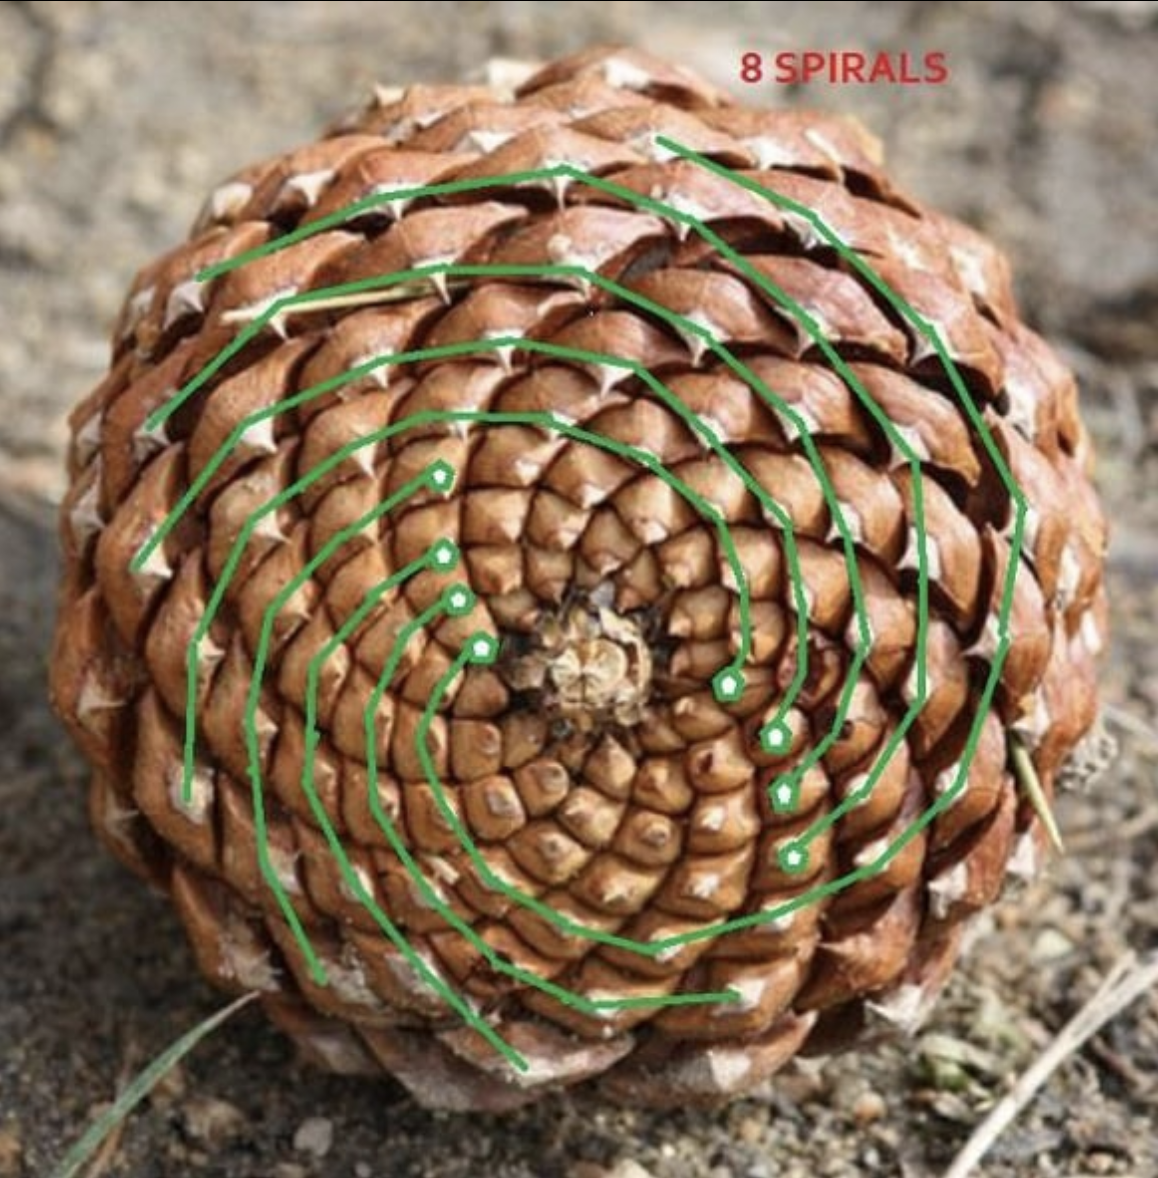
\includegraphics[width=3.68cm]{figure/pinecone.png}\\
                https://www.journals.uchicago.edu/toc/an/current,
 Robert Dryja

	\end{figure}
 \myblue{Emergence is a holistic / gestalt phenomenon. Even
 if there is a straightforward mathematical explanation for
 an emergent phenomenon, it can still make sense to
 distinguish it from subjectively non-emergent phenomena.}

\vfill

\end{frame}


\begin{frame}{counter counter argument (2)}

\vfill

%
\begin{itemize}
\item \ques Have you had a personal emergence experience
  with AI or do you think you will have one in the future?

%  What was your emergence moment with LLMs?
%\item Subjectively, there was clearly some form of ``psychological'' emergence
%when GPT3 and InstructGPT came out (several other models
%as well)

% overall the transition from n-gram language models to
% large neural language models was a quantum leap

%
\end{itemize}


\vfill

\end{frame}

\begin{frame}{Back to finetuning}

\vfill

%
\begin{itemize}
\item \ques You are working at a telecommunications
company. You are given the task of converting a German manual from
polite form (``Wir sind jederzeit unter der folgenden
Nummer fuer Sie erreichbar'') to familiar form
(``Wir sind jederzeit unter der folgenden
Nummer fuer Dich erreichbar''). How would you do this?

\end{itemize}


\vfill

\end{frame}


% ------------------------------------------------------------------------------

% \begin{frame}{Summary}

% \vfill

% \begin{itemize}
%     \item Can we improve model architectures?
%     \item Can we improve data quality and quantity? 
%     \item Better prompting.
%     \item Frontier tasks. 
%     \item Why do emergent abilities occur, and can we predict them? 
% \end{itemize}

% \vfill

% \end{frame}

% ------------------------------------------------------------------------------


%%%%%%%%%%%%%%%%%%%%%%%%%%%%%%%%%%%%%%%%%%%%%%%%%%%%%%%%%%%%%%%%%%
\section{DeepSeek Reasoning}
% Source: DL4NLP chapter09-llm/slides-94-deepseek.tex
%%%%%%%%%%%%%%%%%%%%%%%%%%%%%%%%%%%%%%%%%%%%%%%%%%%%%%%%%%%%%%%%%%
% \input{newway}  % missing in DL4NLP source repo; see order.txt


\begin{frame}{Sources}

\vfill

\begin{itemize}
    \item First major open
    reasoning LM (as opposed to proprietary closed):
    DeepSeek 
\item \citebutton{DeepSeek-AI, 2025}{https://arxiv.org/abs/2501.12948}
\item \citebutton{Nature, 2025}{https://www.nature.com/articles/s41586-025-09422-z}
\end{itemize}

\vfill

\end{frame}

\begin{vbframe}{Data for SFT: 40B tokens!}

\vfill

\begin{figure}
    \centering
    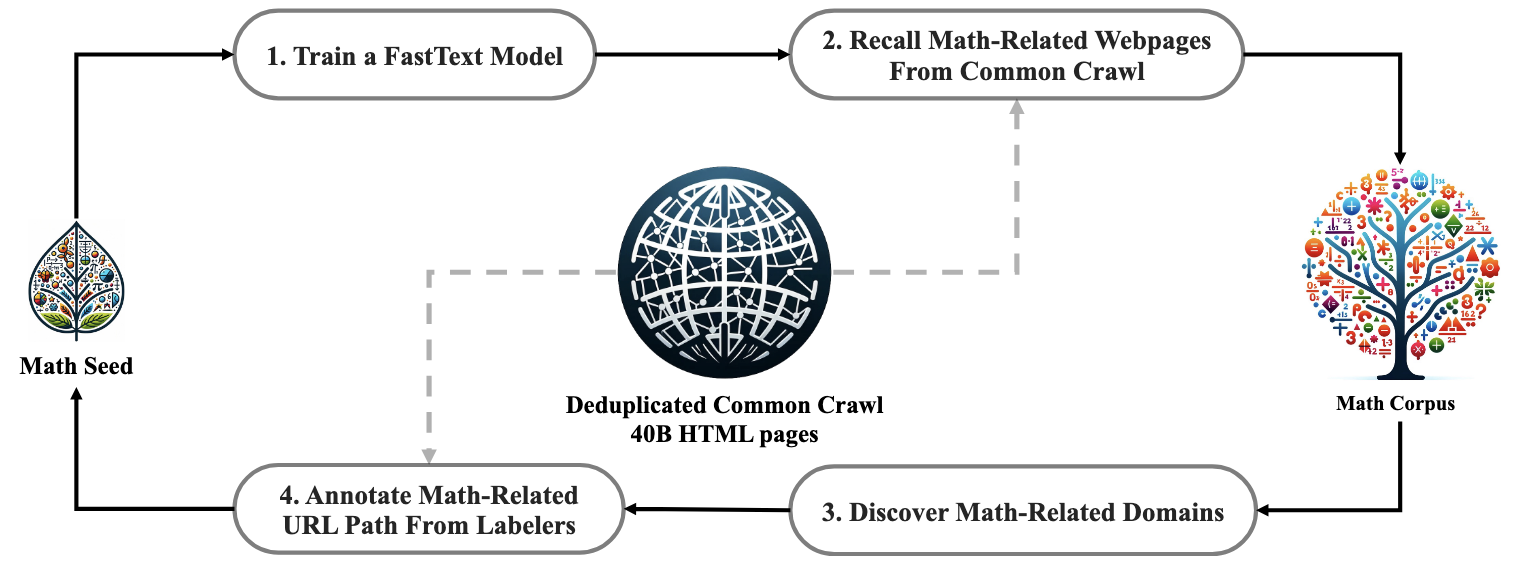
\includegraphics[width=12cm]{figure/deepseekmath.png}
\end{figure}

\citebutton{DeepSeekMath, 2024}{https://arxiv.org/pdf/2402.03300}

\vfill

\end{vbframe}


% inlined from DL4NLP chapter09-llm/reinforce.tex
\begin{vbframe}{Reinforcement learning}

\vfill

\begin{itemize}
\item In reinforcement learning, an agent takes a sequence
    of actions towards a goal and gets feedback on the
    success of that sequence at the end.
    \item Details: Next lecture
    \item For reasoning trajectories, the feedback is:
    correct or incorrect.
\item (thanks to Emma Brunskill) \begin{tabular}{l@{\hspace{0.2cm}}ll}
& supervised learning & reinforcement learning\\\hline
goal&optimal predictor & optimal policy\\ 
learn from experience? & yes & yes\\
generalization? & yes & yes\\
feedback & rich (each token) & sparse (in/correct)\\
feedback when? & immediately & delayed\\
exploration? & no & yes
\end{tabular}

\end{itemize}

\vfill

\end{vbframe}



\begin{frame}{Reasoning traces: Format}

\vfill
\begin{itemize}
\item 
The User asks a
question and the Assistant solves it.
\item The Assistant first
thinks about the reasoning process ``in its mind'' and then
provides  the answer to the User.
\item The reasoning process and
answer are enclosed within <think>...</think> and
<answer>...</answer> tags
\item \texttt{<think> reasoning process here </think>}
\item \texttt{<answer> answer here </answer>}
\item ``We intentionally limit our constraints to this
structural format, avoiding any content-specific biases to
ensure that we can accurately observe the natural
progression of the model during the RL process.''
\item So this is not a few-shot approach!
\end{itemize}

\vfill

\end{frame}

\begin{vbframe}{Example of a reasoning trace}

\vfill

\begin{tabular}{lp{2cm}}
    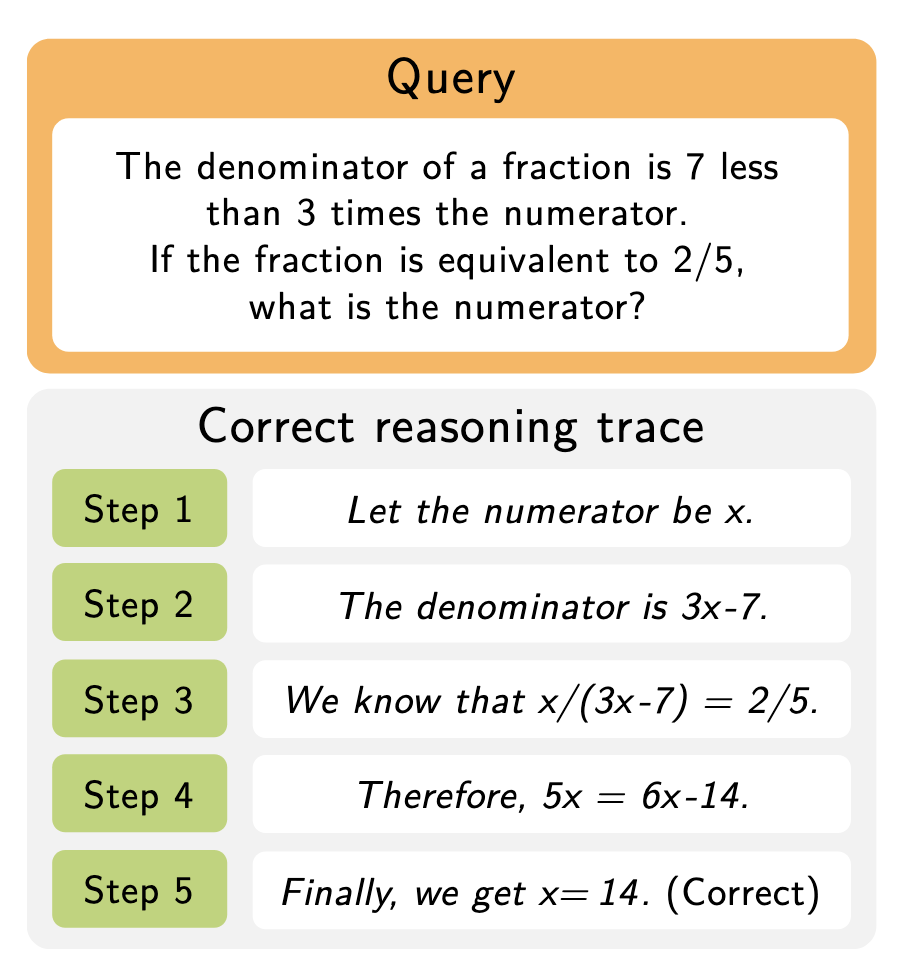
\includegraphics[width=5.78cm]{figure/reasoning,trace}&
\vspace{-5cm} \ques Is this chain of thought few-shot prompting? 
\end{tabular}

\vfill

\end{vbframe}


\begin{frame}{Automatic, non-human rewards\\ for
    LM-generated reasoning traces}

\vfill

\begin{block}{}
Accuracy rewards evaluate whether the response is
correct. For
example, in the case of maths problems with deterministic
results,
the model is required to provide the final answer in a
specified format
(for example, within a box), enabling reliable rule-based
verification of
correctness. Similarly, for code competition prompts, a
compiler can
be used to evaluate the responses of the model against a
suite of predefined test cases, thereby generating objective feedback on correctness.
\end{block}

\vfill

\end{frame}



\begin{vbframe}{Automatic verifier/verifiable rewards: AIME example}

\vfill

\begin{figure}
    \centering
    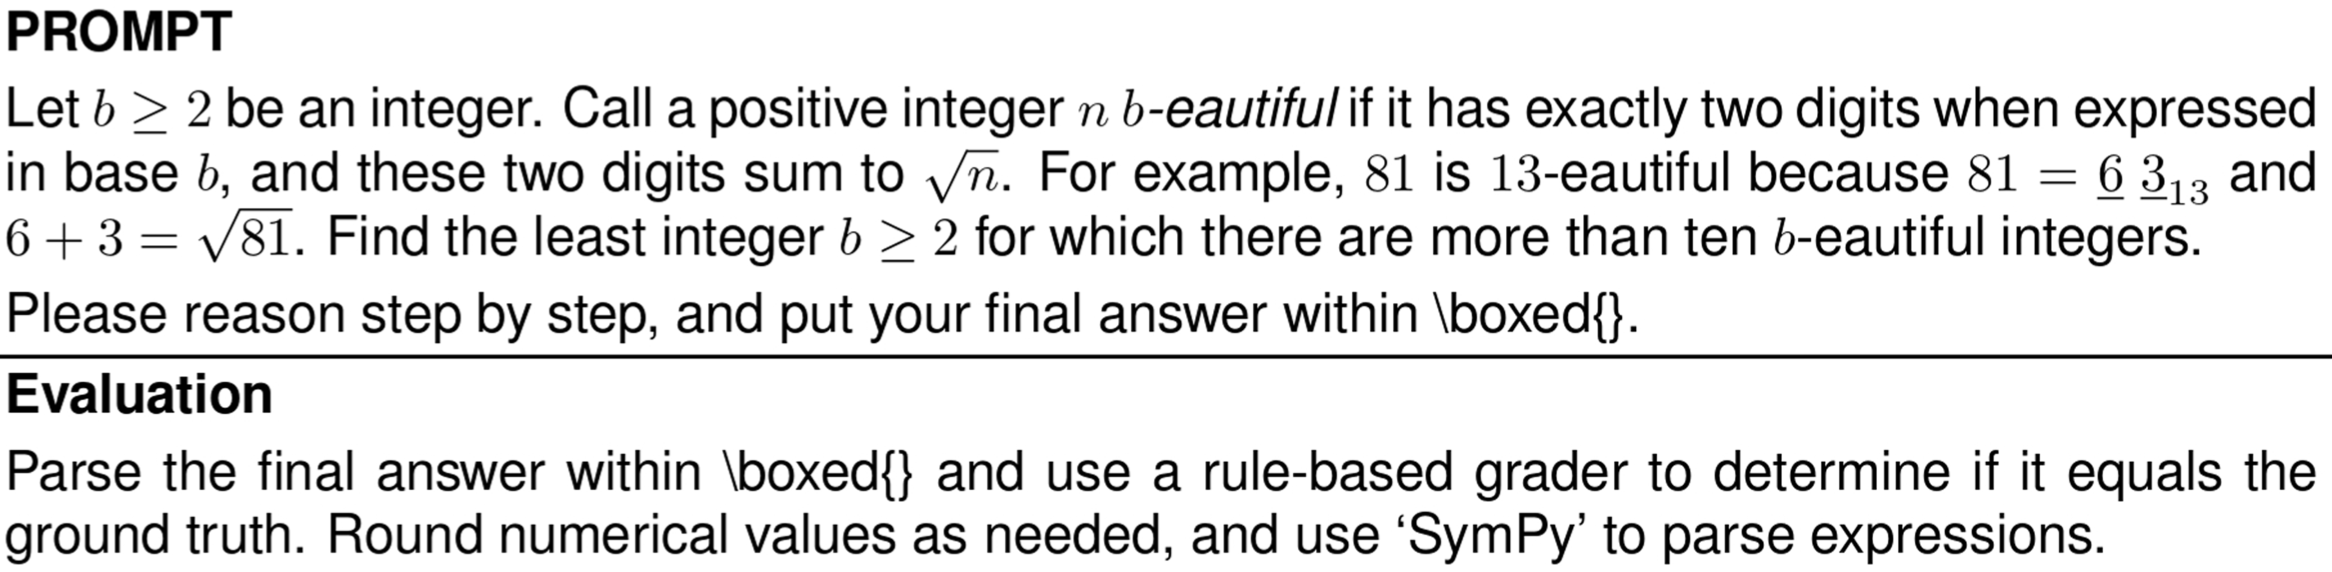
\includegraphics[width=11.5cm]{figure/aime,example}
\end{figure}

\vfill

\end{vbframe}


\begin{frame}{Inference time scaling}

\vfill

\begin{itemize}
    \item For a hard problem, it often helps to think for a
    long time to come up with the solution.
    \item Inference time scaling: teach the model to think
    for a while before giving the answer.
    \item Here, thinking means that the model produces
    potentially long output, the reasoning trace, that leads
    to the correct answer.
\end{itemize}

\vfill

\end{frame}



\begin{frame}{What elements of reasoning are learned?}

\vfill

\begin{itemize}
\item dynamic strategy adaptation
    \item self-verification
    \item reflection
    \item backtracking
    \item reasoning traces are getting longer
\item exploration of alternative approches
\item diverse and sophisticated reasoning behaviors
\end{itemize}

\vfill

\end{frame}


\begin{vbframe}{Aha moment}

\vfill

\begin{figure}
    \centering
    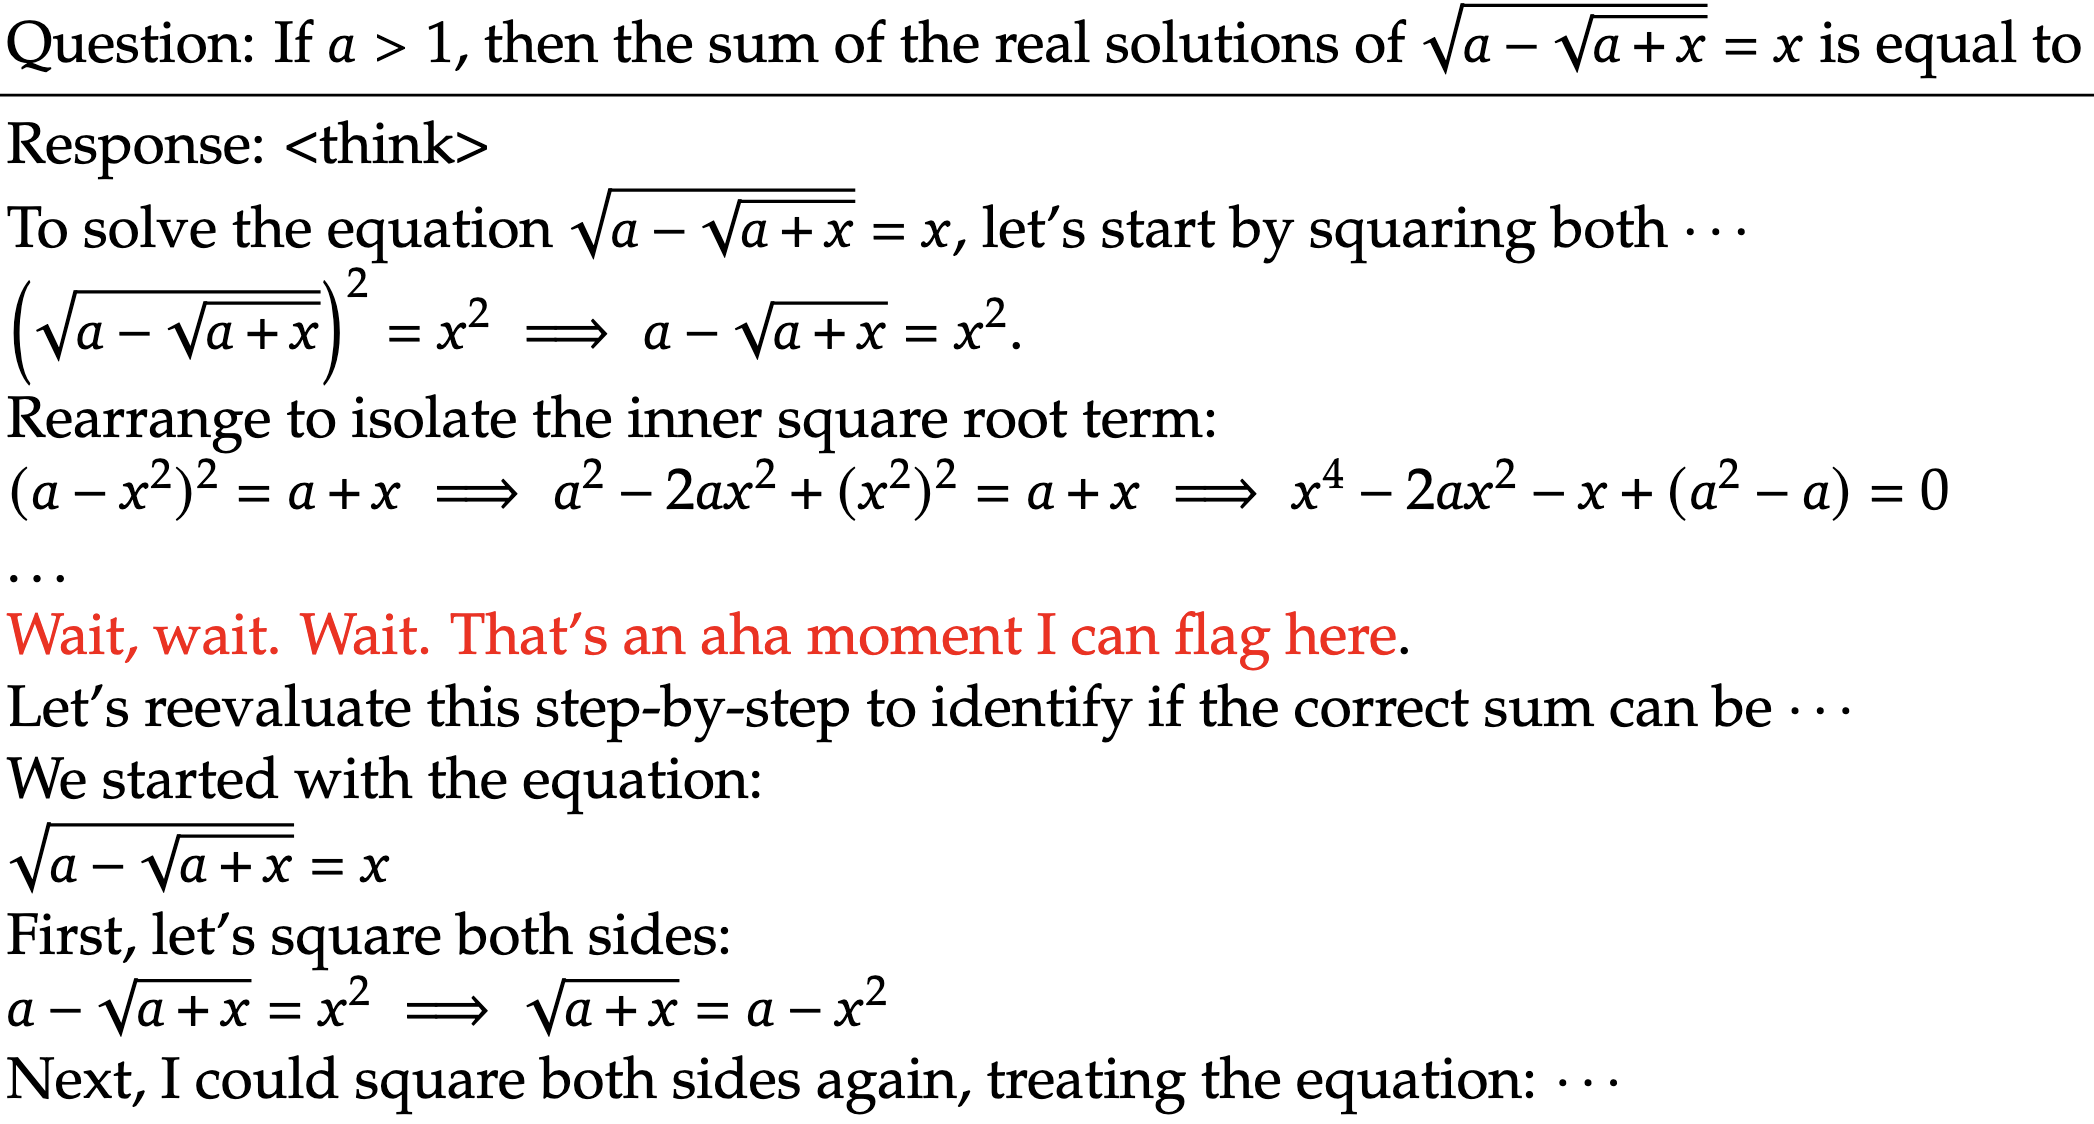
\includegraphics[width=10cm]{figure/ahamoment}
\end{figure}

\vfill

\end{vbframe}

\begin{vbframe}{Another example for Aha moment}

\vfill

\begin{figure}
    \centering
    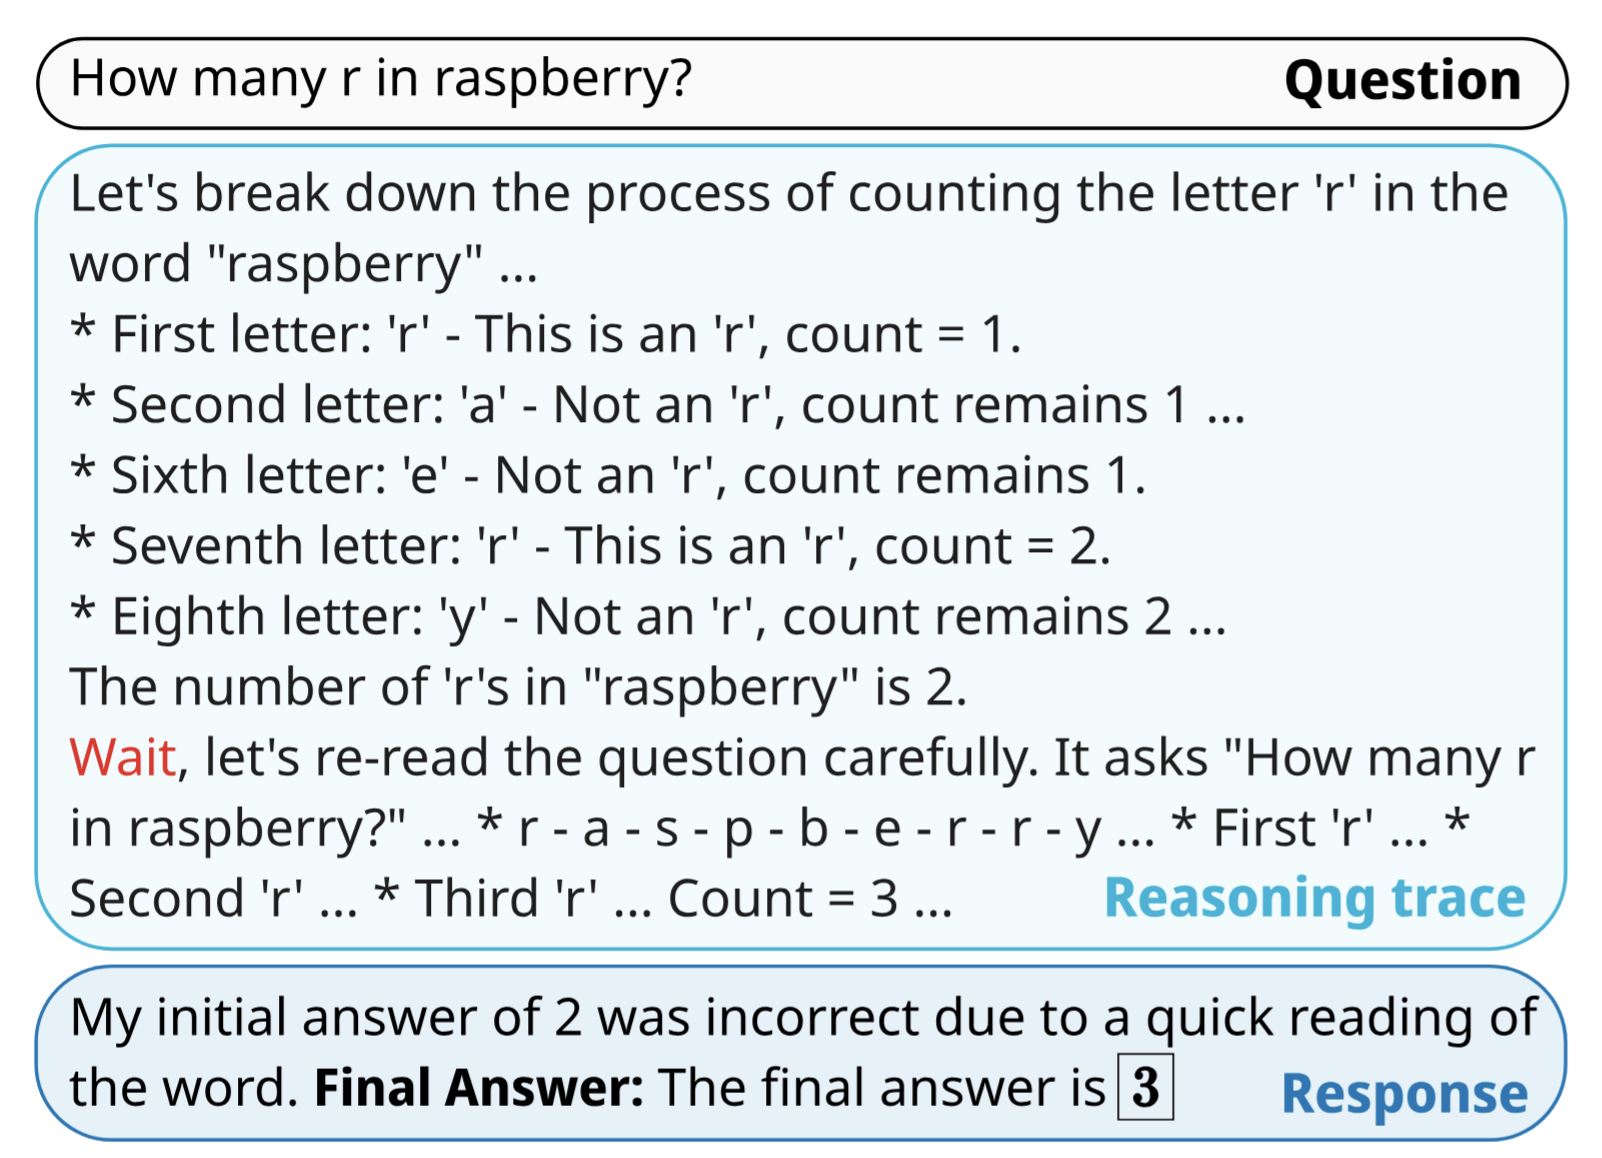
\includegraphics[width=8.50cm]{figure/raspberry,wait}
\end{figure}

\vfill

\end{vbframe}


\begin{vbframe}{The rise of reflective terms}

\vfill

\begin{tabular}{ll}
    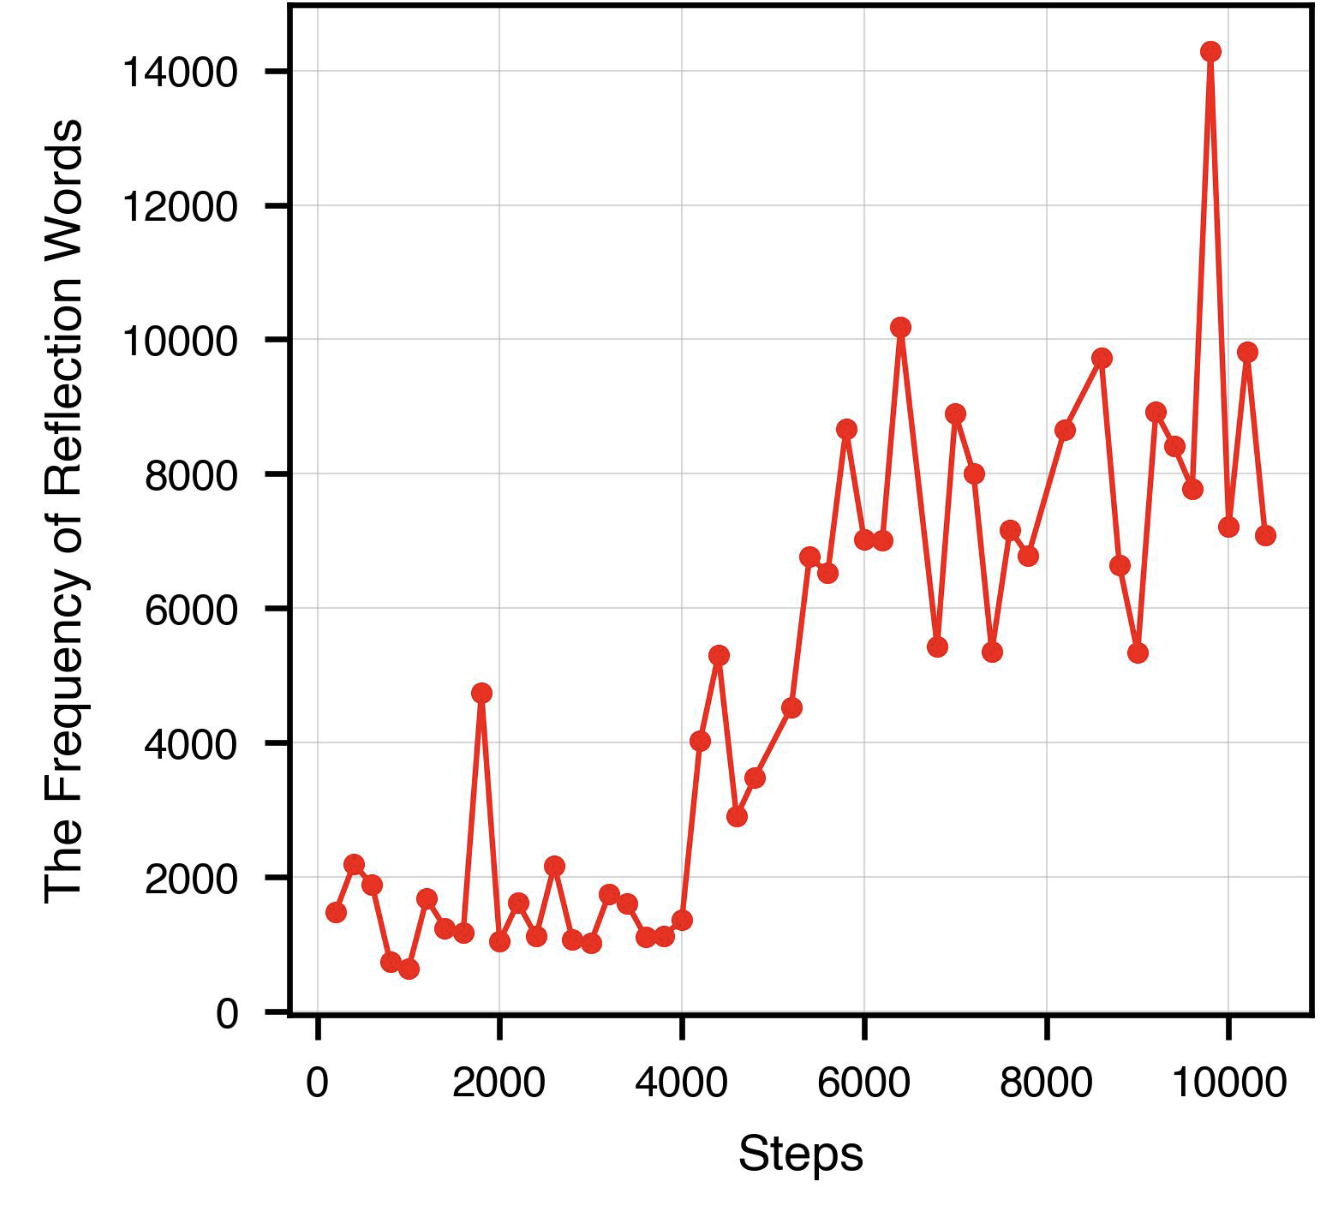
\includegraphics[width=6.80cm]{figure/reasonling}
  \begin{minipage}[b]{3cm}
Frequency of
 reflective terms
(‘wait’, ‘mistake’, ‘however’,
 ‘but’, ‘retry’, ‘error’,
 ‘verify’, ‘wrong’, ‘evaluate’, ‘check’)
in model output during
 training
\end{minipage}
\end{tabular}

\vfill

\end{vbframe}


\begin{vbframe}{Accuracy AIME: Above human average}

\vfill

\begin{figure}
    \centering
    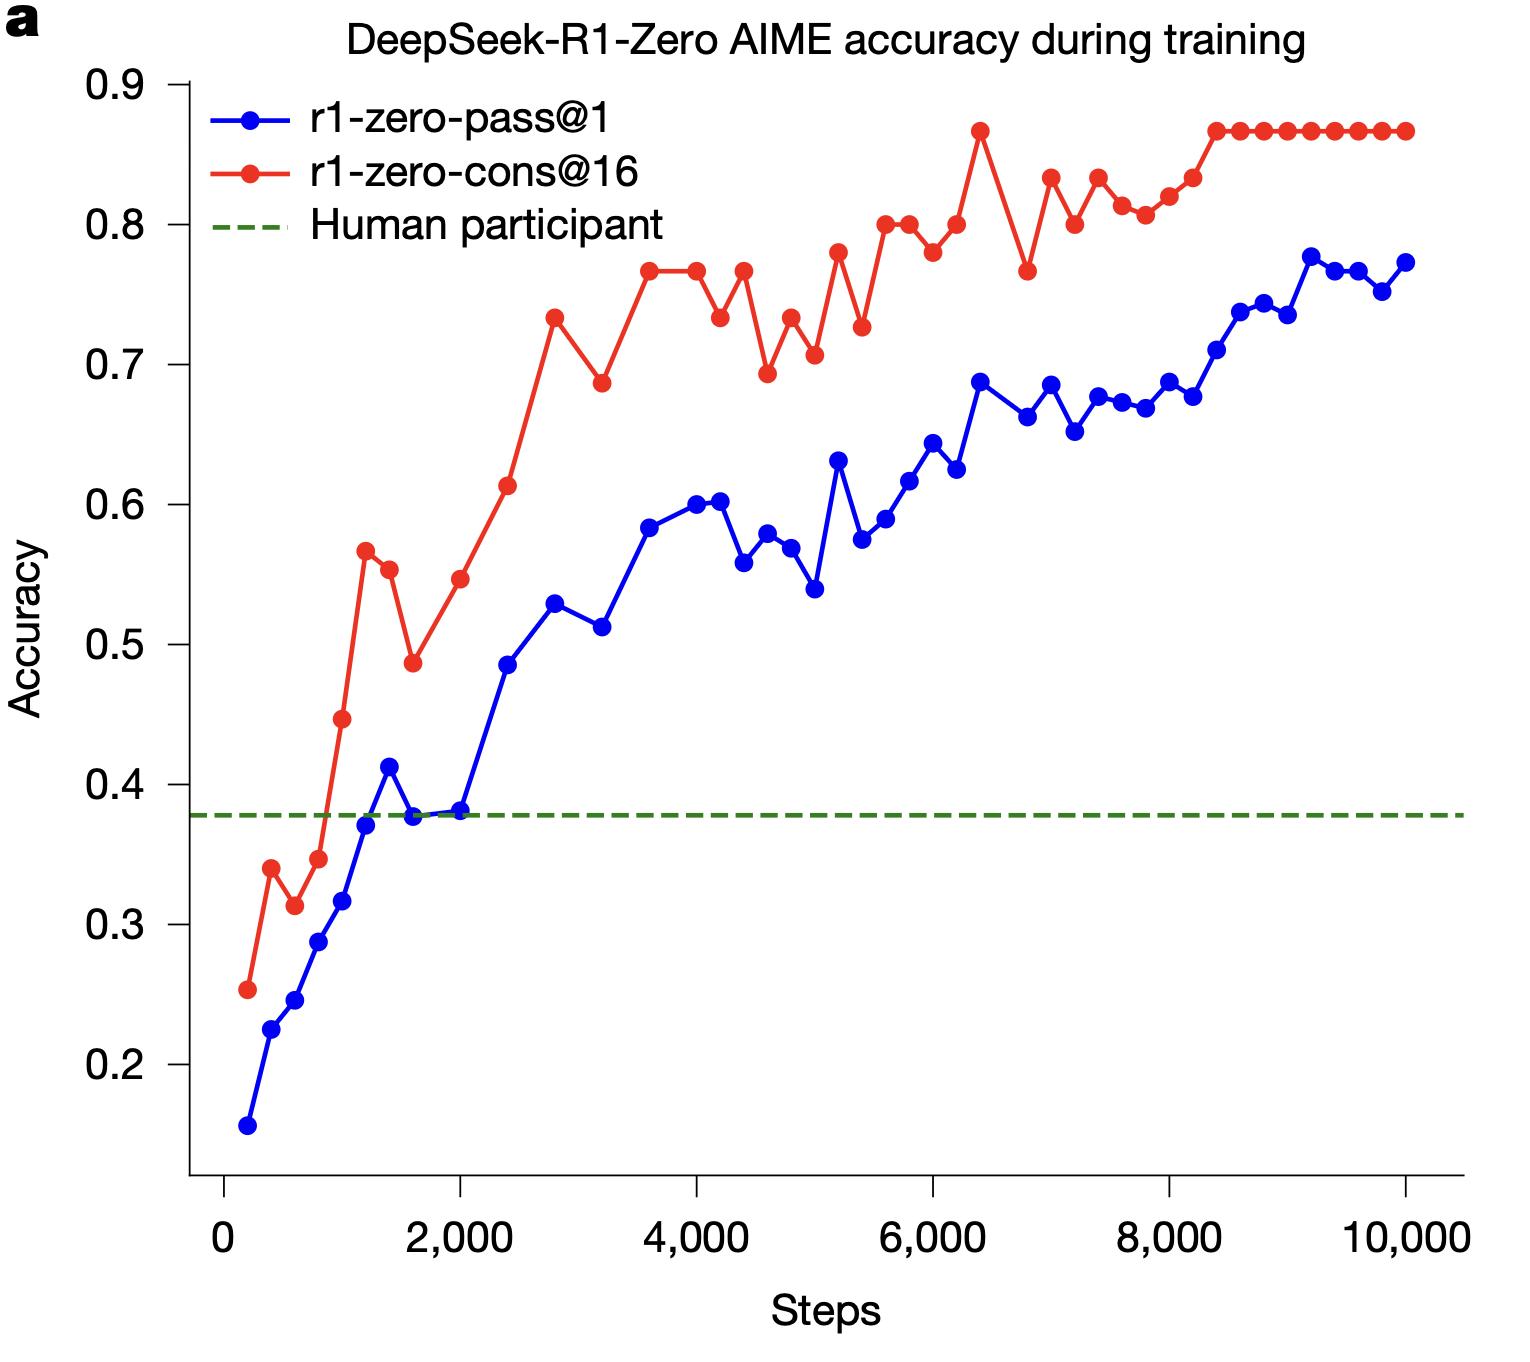
\includegraphics[width=6.80cm]{figure/accuracy,aime.png}
\end{figure}

\vfill

\end{vbframe}


\begin{vbframe}{R1 scaling: Without explicit length signal}

\vfill

\begin{figure}
    \centering
    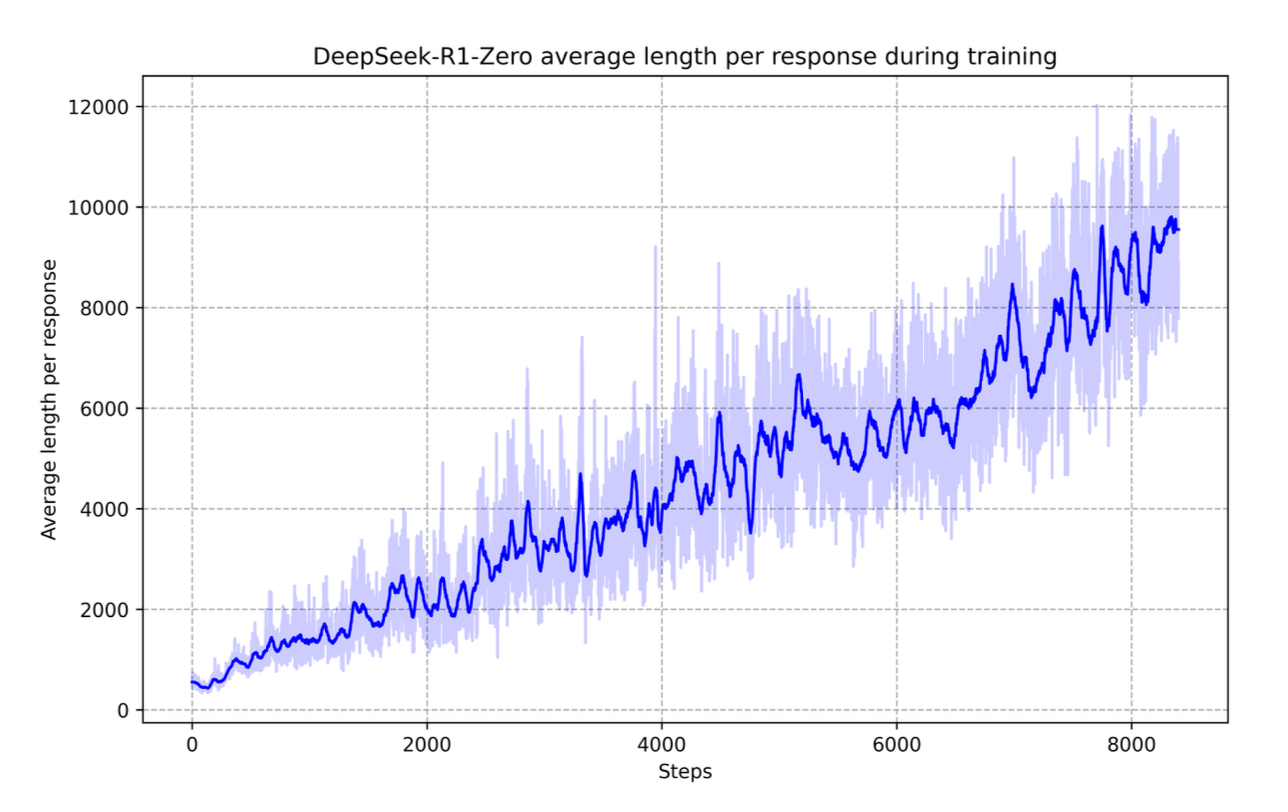
\includegraphics[width=10cm]{figure/r1scaling}
\end{figure}

\vfill

\end{vbframe}



\begin{vbframe}{Unfaithfulness of LMs to true reasoning}

\vfill

\begin{figure}
    \centering
    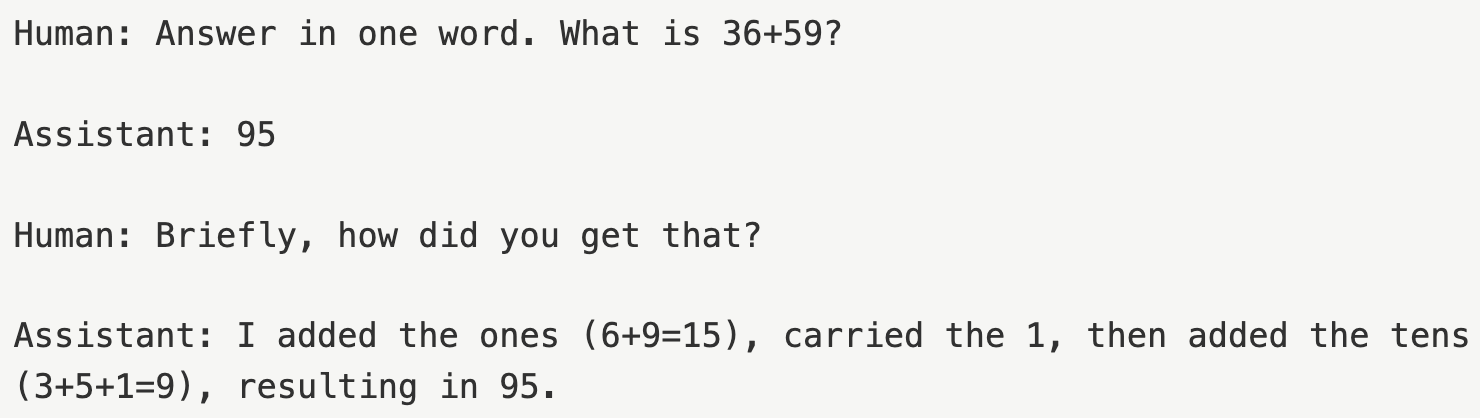
\includegraphics[width=12cm]{figure/sixplusnine,0.png}
\end{figure}

\vfill

\end{vbframe}

\begin{vbframe}{Unfaithfulness of LMs to true reasoning}

\vfill

\begin{figure}
    \centering
    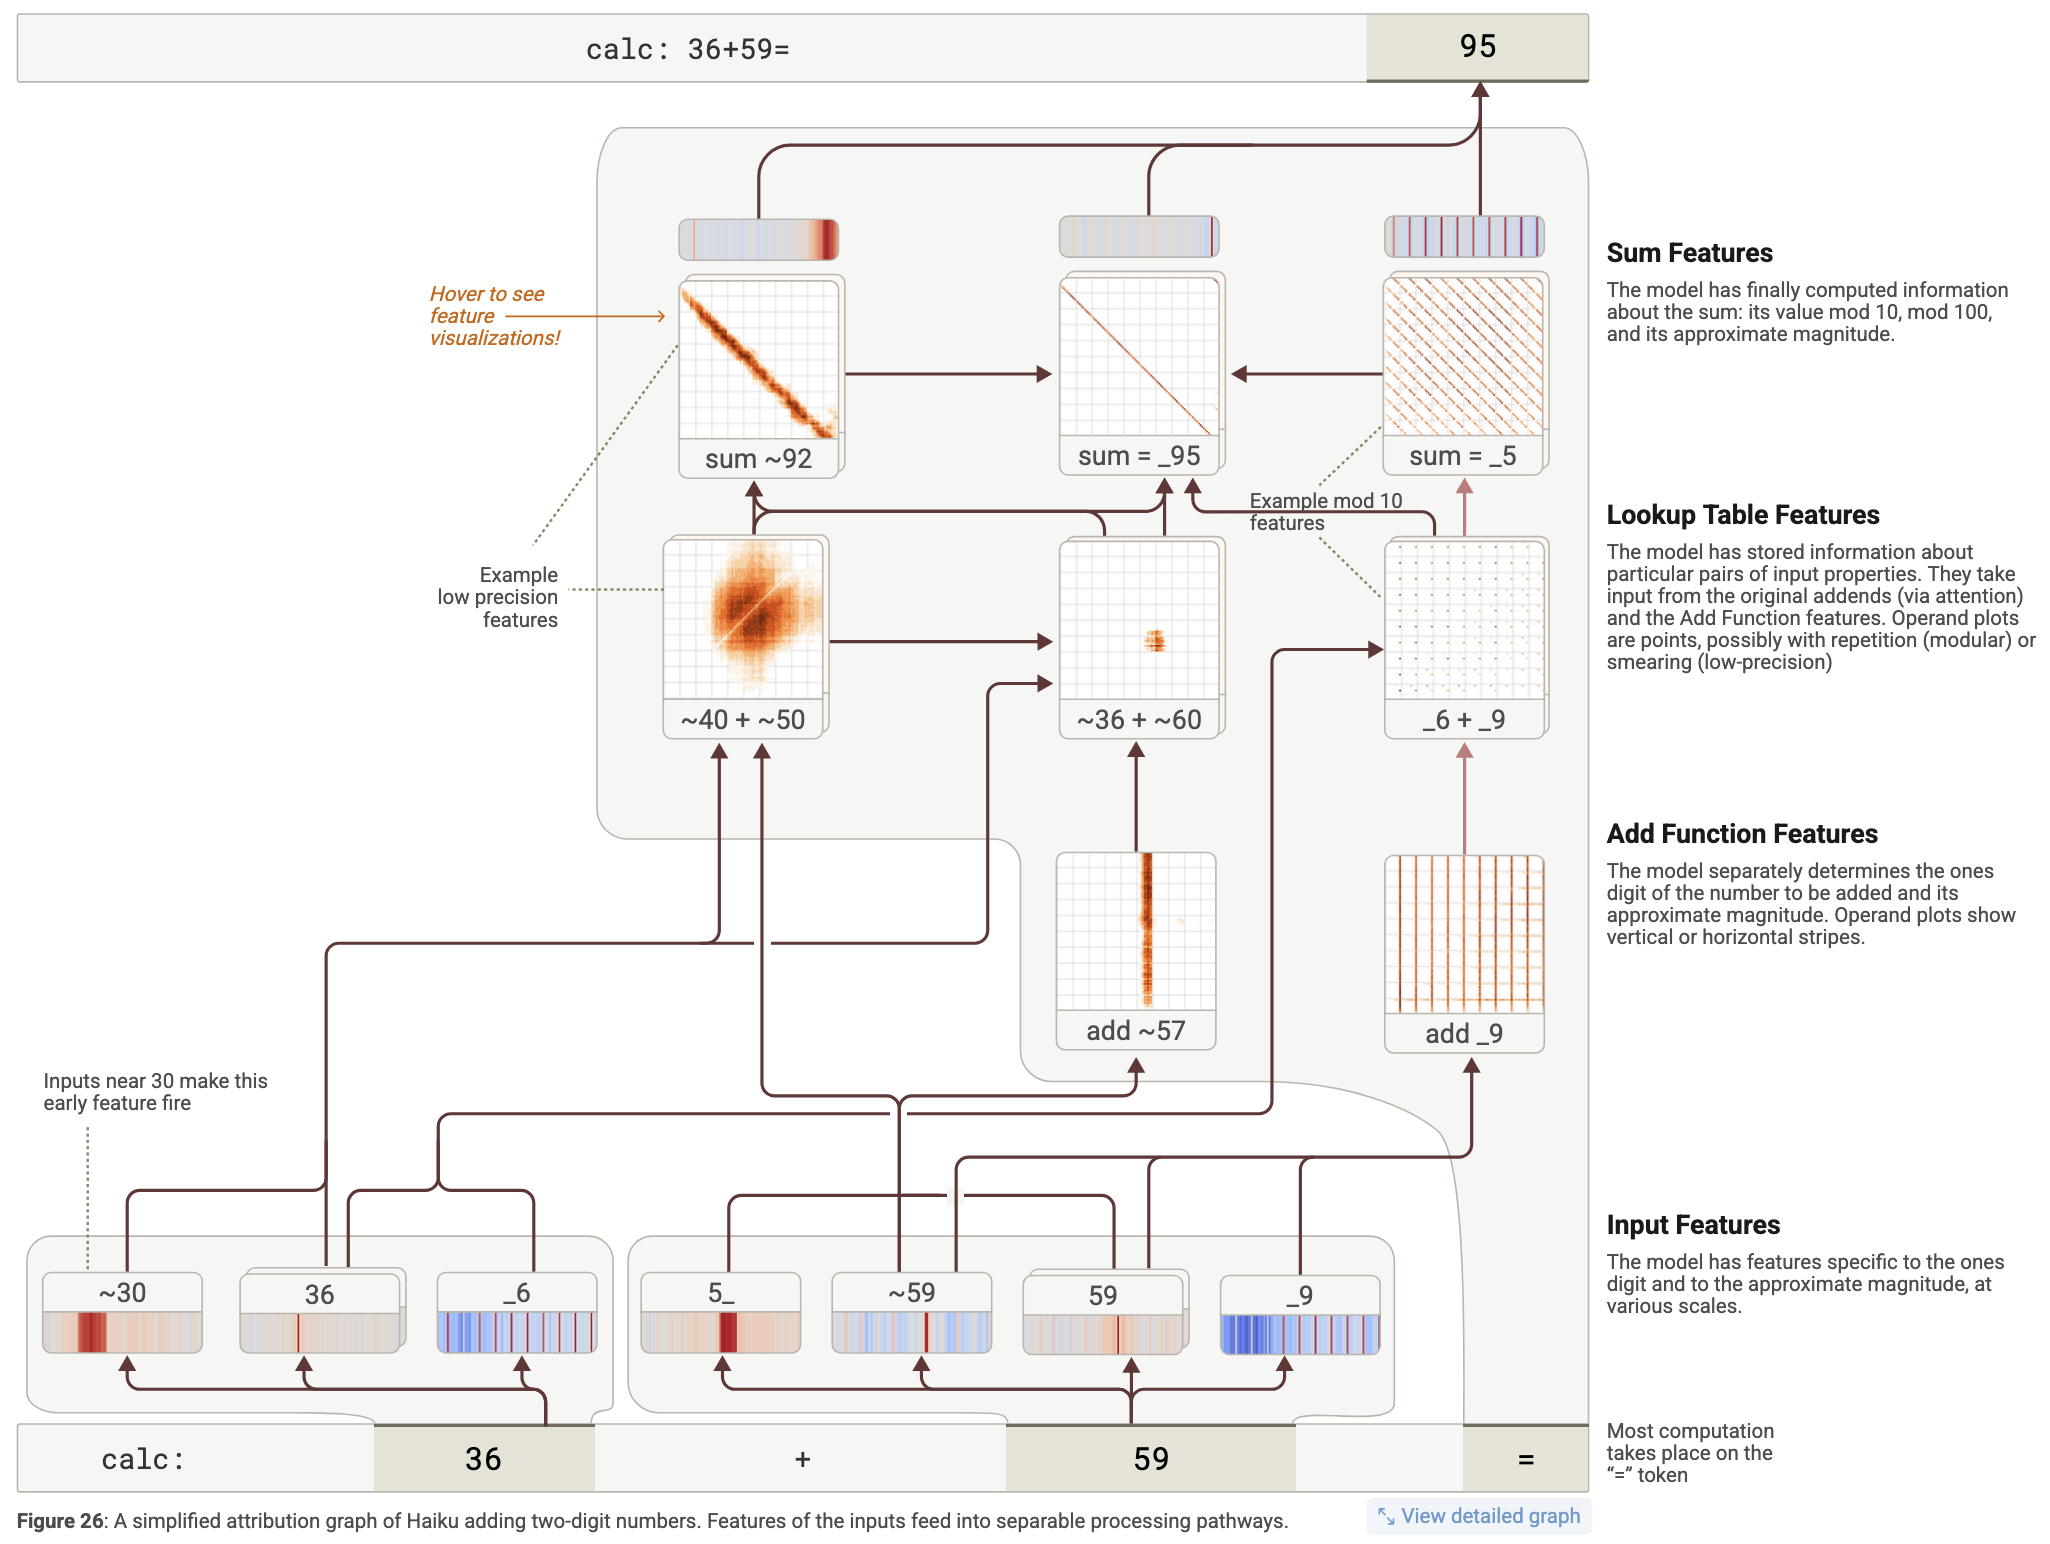
\includegraphics[width=7.65cm]{figure/sixplusnine,1.png}
\end{figure}

\vfill

\end{vbframe}



\begin{frame}{Things we have not covered}

\vfill

\begin{itemize}
\item use an eco system of several models:\\
for distillation, generation, verification
\item some ``light'' human post-editing of training data
\item rejection sampling:\\ keep only high-quality,
    high-confidence training data
\item apart from math, they also do this for code and other domains
\item major hardware optimization work
\item claim: cost of training $<$ 1 000 000 million dollar
\end{itemize}

\vfill

\end{frame}

% \input{newway}  % missing in DL4NLP source repo; see order.txt


%%%%%%%%%%%%%%%%%%%%%%%%%%%%%%%%%%%%%%%%%%%%%%%%%%%%%%%%%%%%%%%%%%
\section{License \& Attribution}
%%%%%%%%%%%%%%%%%%%%%%%%%%%%%%%%%%%%%%%%%%%%%%%%%%%%%%%%%%%%%%%%%%

\begin{vbframe}{License \& Attribution}
\begin{itemize}
\item \textbf{Single source.} All content is taken from \textbf{Deep Learning for NLP (DL4NLP)}, SLDS, LMU Munich, chapters 7 (\textit{Generative Pre-Trained Transformers}), 8 (\textit{Decoding Strategies}) and 9 (\textit{Large Language Models}), in the source's own order --- licensed \textbf{CC BY 4.0}: \url{https://creativecommons.org/licenses/by/4.0/}.
\item Figures are reproduced as they appear in DL4NLP, with the attributions DL4NLP itself gives.
\end{itemize}
\end{vbframe}

\endlecture
\end{document}
